\chapter{CENSUS ANNOTATION} \label{chapter:ca}

\noindent Automated photographic censusing is sensitive to how its annotations are selected and why they have matched.  When the ID curation process encounters incomparable pairs or incidental matching, it can create errors in the ID database that must be fixed with human interaction, as we have discussed.  Fortunately, the adverse effects on automation and accuracy can be mitigated when 1) the ID curation process only considers comparable annotations and 2) the automated ranking algorithm is forced to compare the appropriate visual information between annotations.  Let us consider a real-world example shown in Figure~\ref{fig:ca-overview} on the next page, with two images (top and bottom) of Gr\'evy's zebra (\textit{Equus grevyi}).  Of the 13 animals seen across both images, only four are valuable to photographic censusing (highlighted as red and blue annotations) because they are universally comparable.  The remaining nine annotations (in dashed green) are either incompatible or too challenging for censusing as they show incorrect viewpoints\footnote{The decision on a preferred viewpoint is arbitrary but needs to be consistent throughout a census.  The right side was preferred for all image collections with Gr\'evy's zebra and reticulated giraffe (\textit{Giraffa reticulata}).  These two species have different patterns on their left and right sides and thus cannot be compared across differing viewpoints.}, are truncated by the edge of the image, or are significantly occluded by other animals or brush.  The middle row of Figure~\ref{fig:ca-overview} shows two comparable annotations (red and blue outline) of the same animal, with matched patterns highlighted in yellow (within the purple dashed ovals) from the HotSpotter~\cite{crall_identifying_2017} algorithm.  If all purple oval regions were artificially blacked out, verifying the pair by hand would be substantially more difficult and would take a human more time to make an accurate decision.  Furthermore, we recognize that the visual information outside the purple rectangles for each annotation is not critical to this verification task.  The pixels outside the purple boxes could have been safely omitted to focus the verifier's attention on the matched area without impacting the ability to make a ``same animal'' decision.

New detection methods are needed that can 1) quickly determine if an annotation is comparable and 2) remove distracting background information by locating the area that is most likely to match for that species.  This chapter introduces the concepts of ``Census Annotation'' (CA) and ``Census Annotation Region'' (CA-R) to address these two problems, and it proposes adding two new machine learning components to the existing detection pipeline:

\begin{enumerate}
    \item \textbf{Census Annotation (CA)} - a binary classifier that determines if an annotation contains a comparable region and produces a confidence score, and
    \item \textbf{Census Annotation Region (CA-R)} - a regression network that restricts an annotation's existing bounding box to only include the comparable region for a given species.
\end{enumerate}

\noindent An annotation is determined to be a Census Annotation if and only if a valid Census Annotation Region can be drawn inside its existing bounding box.  Furthermore, A Census Annotation Region\footnote{Census Annotation Regions may be referred to as ``CA-R'' or ``CA Regions'' in this discussion, as needed, for clarity.} must contain enough visual ID information to prevent the possibility of an incomparable match decision (for a given ranking algorithm). Thus, by definition, if a CA-R bounding box cannot be drawn for an annotation, it cannot be a CA.  Furthermore, if two CA Regions are incomparable, at least one of the annotations is not a valid CA.  For example, the hip and shoulder chevron (purple dashed ovals in Figure~\ref{fig:ca-overview}) are required for Gr\'evy's zebra annotations to be considered comparable. Missing either of those two areas makes the annotation less likely to reliably match, increasing the possibility of an incomparable decision and the ultimate need for human intervention.  To prevent this, the CA-R region for that species must clearly contain both of these regions.

\begin{figure}[!t]
    \begin{center}
        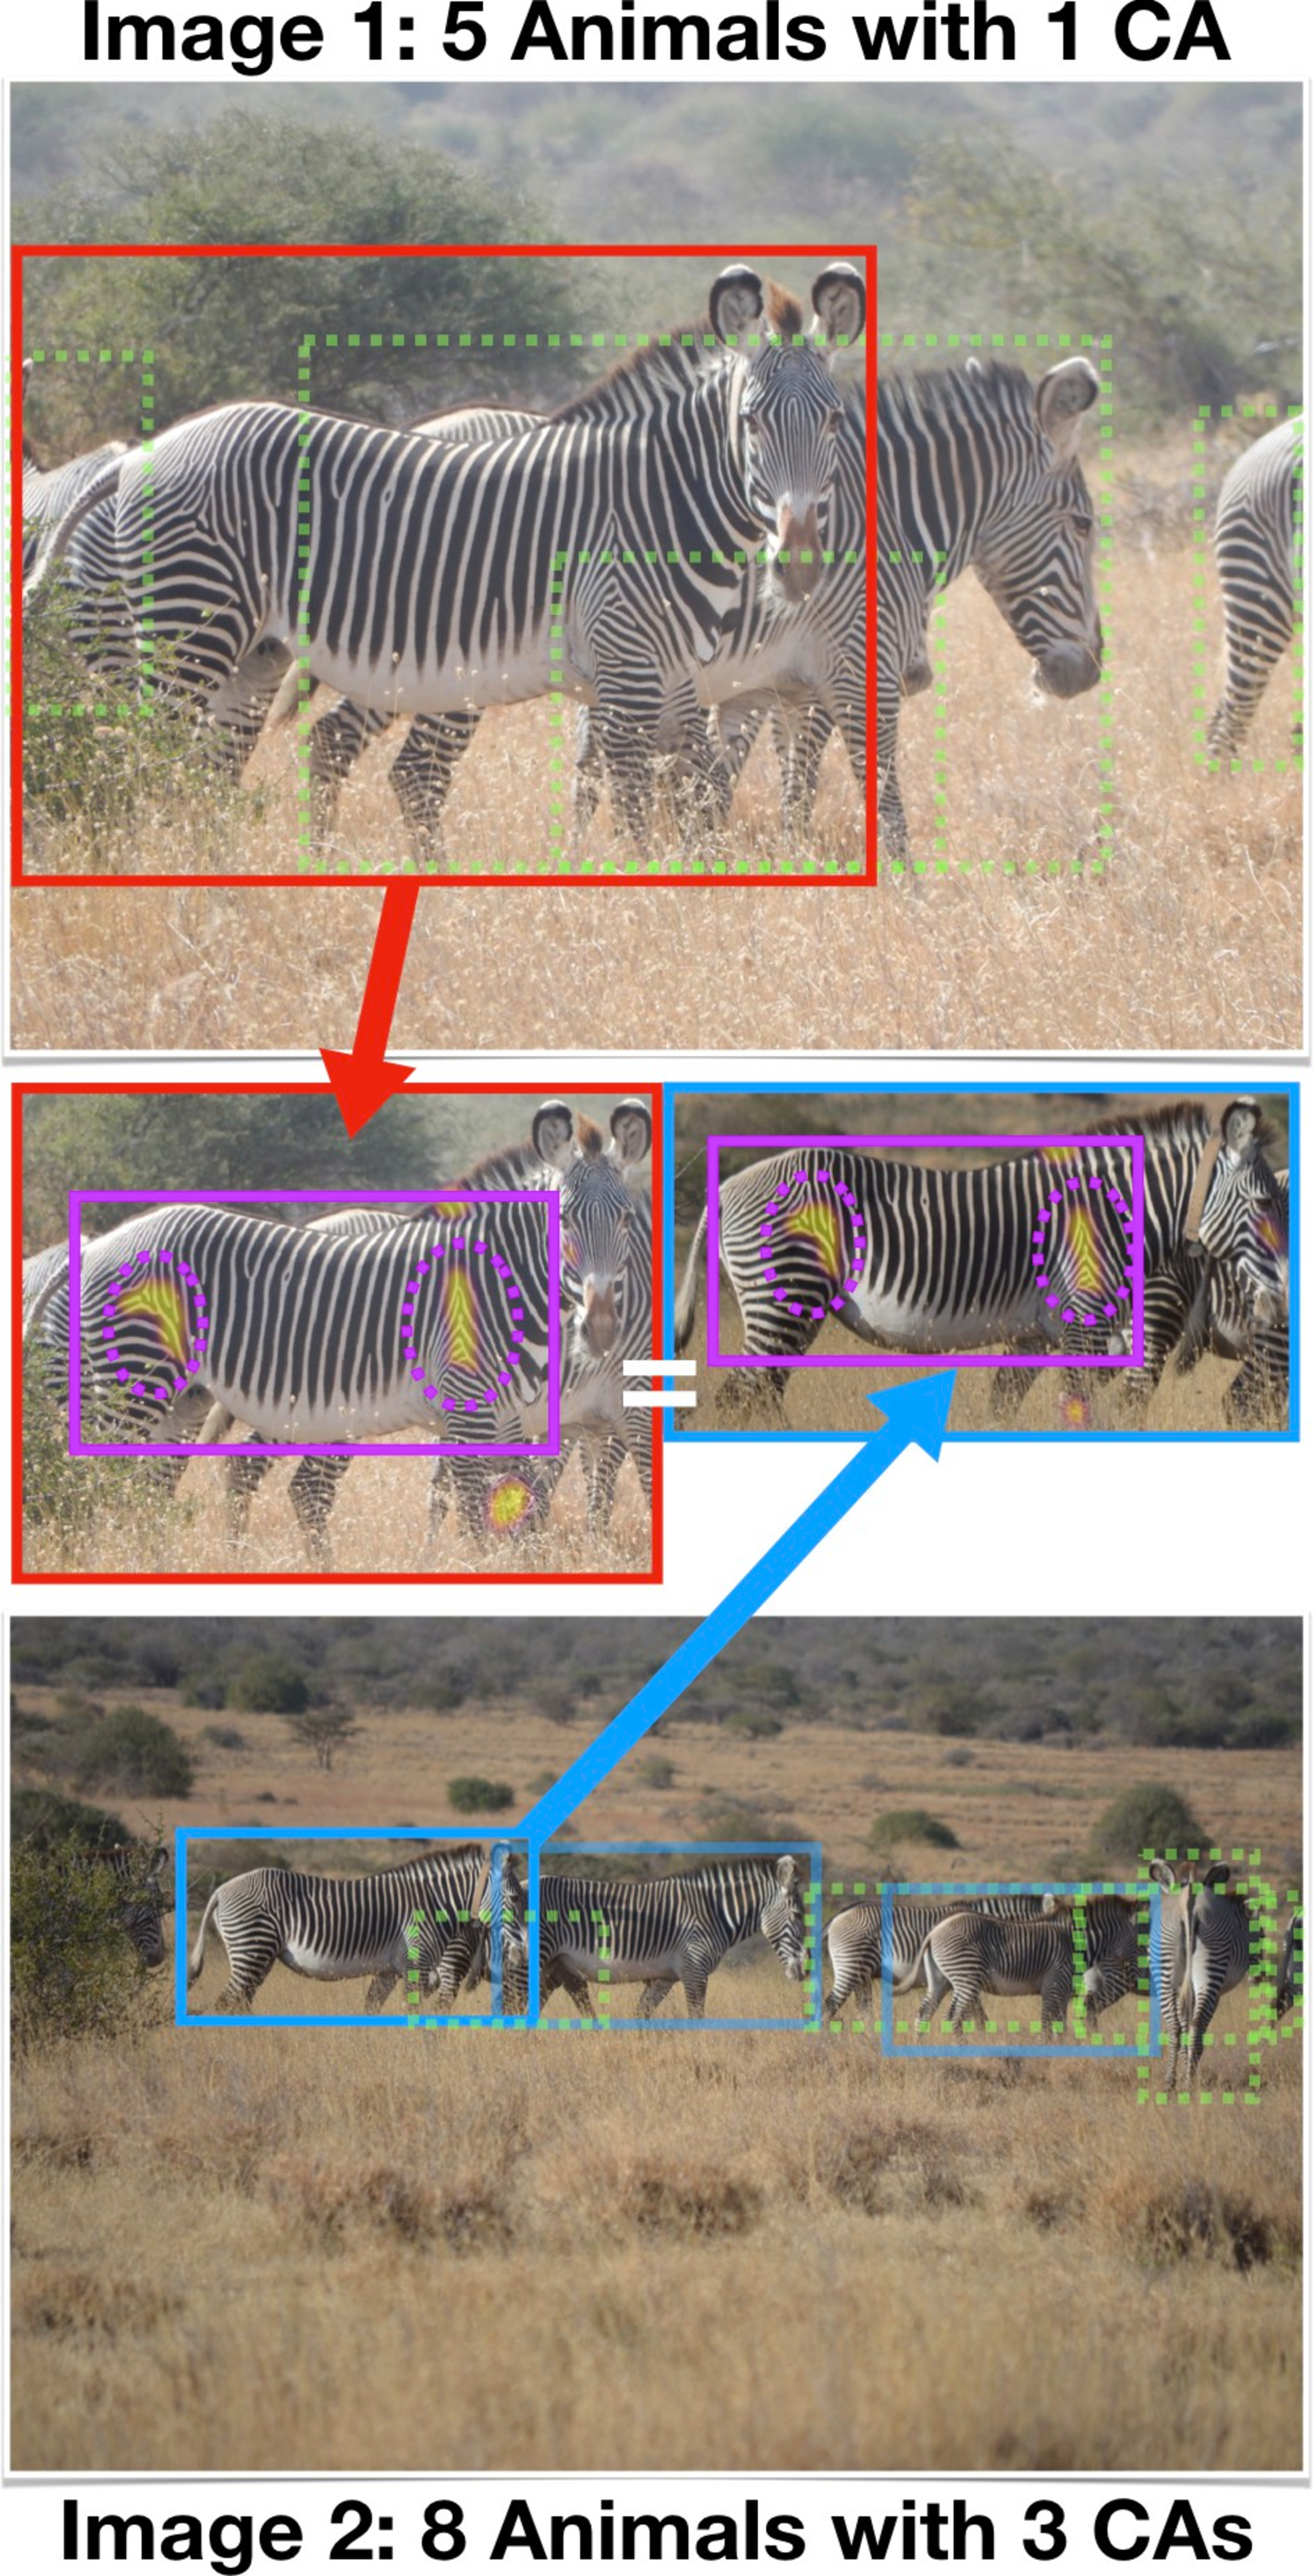
\includegraphics[width=0.58\linewidth]{resources/ca-example.pdf}
    \end{center}
    \caption{An example of identification matching with two Census Annotations.  Image 1 (top) shows a Census Annotation (CA) in red, which captures the same individual as the blue Census Annotation in Image 2 (bottom).  The matched CAs (purple boxes) both contain the distinct chevron and hip regions (ovals) that commonly match by ID.}
    \label{fig:ca-overview}
\end{figure}

The remaining sections of this chapter present a description of the methods and an analysis of both Census Annotations and Census Annotation Regions. First, a dataset for training both of these components is presented for Gr\'evy's zebra and reticulated giraffe, which were the species of interest for the Great Gr\'evy's Rally in 2018 (discussed in Chapter~\ref{chapter:censusing}).  A user study is also performed on how accurately and quickly humans can distinguish match pairs between ``normal'' detected annotations, CAs, and CA-Rs.  Using CAs and CA-Rs with ID curation also positively impacts the performance of automated verifiers, and analysis on training stability and score separability is provided.  The discussion then turns to incidental matching and how CA-R can reduce the rate of photobombs and scenery matches by eliminating the background information that causes these types of errors.  Lastly, automated simulations are used to measure how much human effort is needed to curate an animal ID database from scratch, with and without CA and CA-R, and demonstrate two crucial results: 1) using CAs and CA-Rs during ID curation results in a substantial increase in automation, 2) the population estimates produced when only CAs and CA-Rs are considered are consistent with the estimate generated when a more comprehensive set of annotations from GZCD (described in Section~\ref{sec:gzcd}) are used.

\section{Census Annotation Dataset}\label{sec:ca-dataset}

Both the Census Annotation and Census Annotation Region components were trained on a dedicated dataset for the problem and are evaluated as stand-alone machine learning approaches, separating them from the photographic censusing experiments later in this chapter and the creation of the GZCD from Chapter~\ref{chapter:overview}.  A collection of 10,229 Gr\'evy's zebra and 2,322 reticulated giraffe annotations were exported from the Great Gr\'evy's Rally 2018 dataset, along with their original images and any other annotations that were also seen in those images.  A reviewer was provided with a grid of annotations in a web interface to select the annotations that were CAs for the respective species.  For this task, a CA was defined as any annotation that clearly showed (i.e., in focus, well lit) a right-side Gr\'evy's zebra with its hip and shoulder region visible.  For a reticulated giraffe, the body region needed to be fully visible (ignoring any ability to see the neck, head, and legs) for its annotation to be considered a valid CA.  Each grid presented 500 annotations, and the reviewer toggled the state for a specific annotation by clicking on an image's thumbnail.  The decisions were saved in bulk for the entire grid, and the process was repeated with subsequent grids of unlabeled annotations until the entire dataset was reviewed.  Once all ground-truth CA decisions were added, a second independent review (by a second person) was performed for all negative ``non-CA'' (NCA) annotations and positive CA annotations, as two separate groups, to cross-check for ground-truth errors.

\begin{figure}[!t]
    \begin{center}
        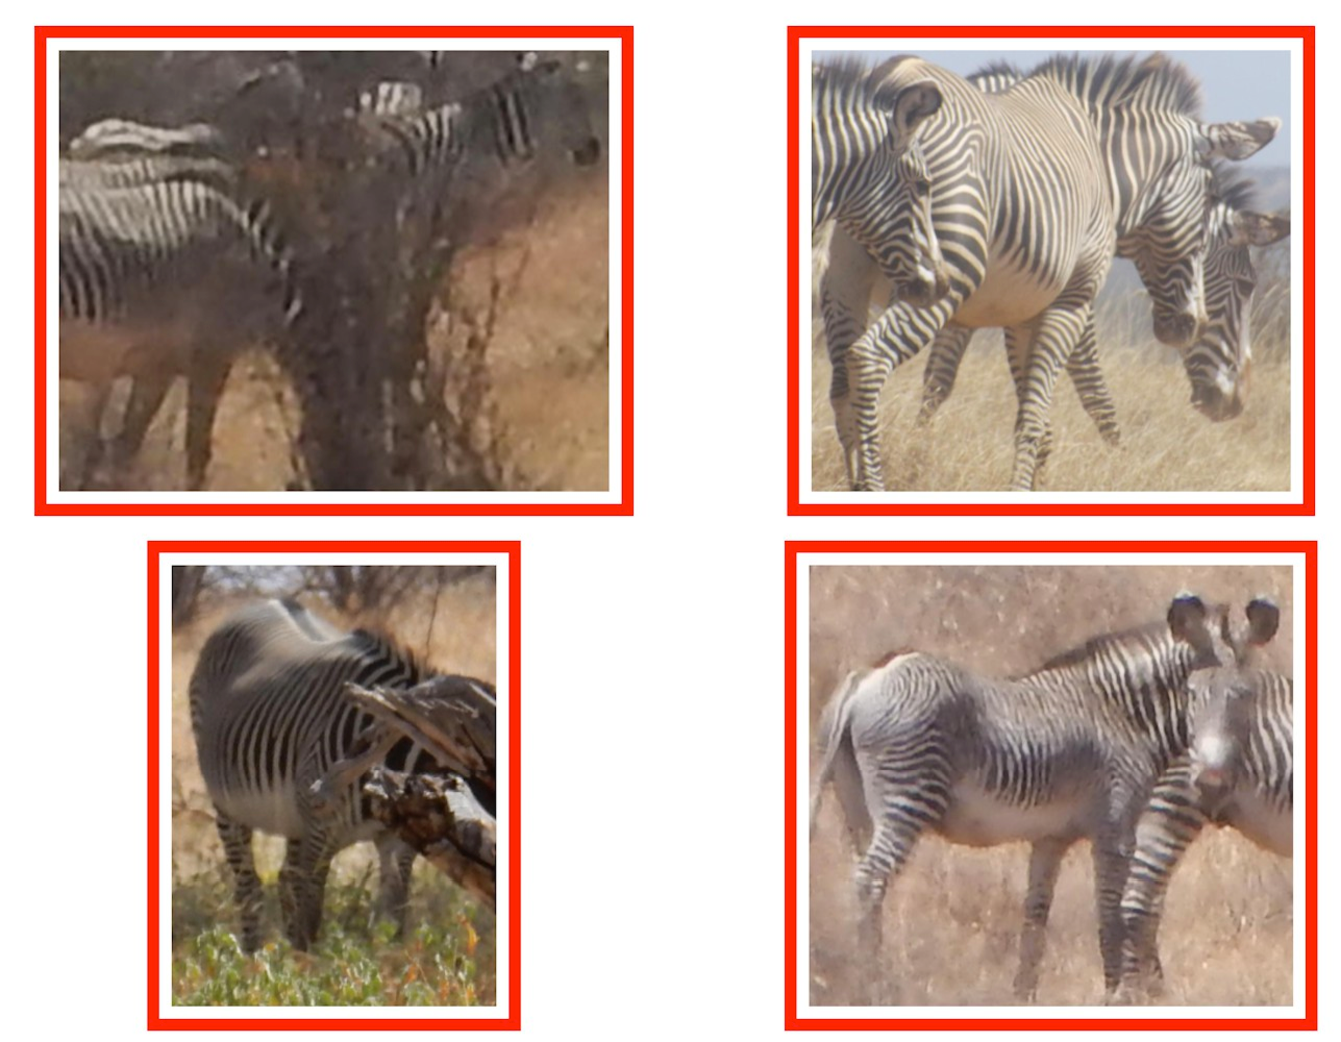
\includegraphics[width=0.45\linewidth]{resources/canonical-no.pdf}
        \hspace{1mm}
        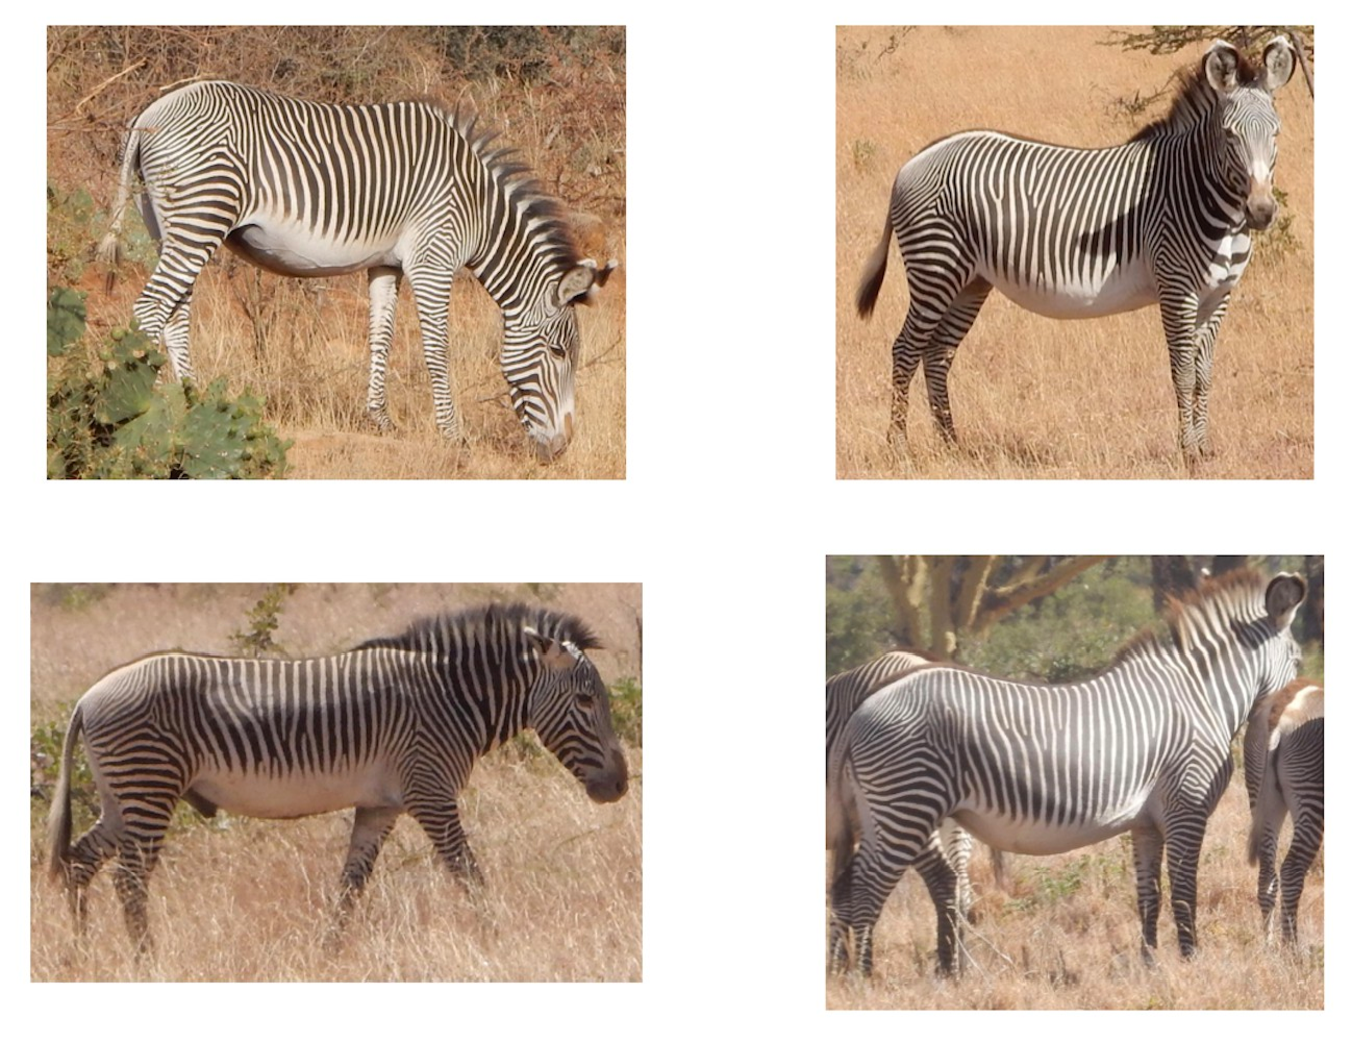
\includegraphics[width=0.45\linewidth]{resources/canonical-yes.pdf}
        \\
        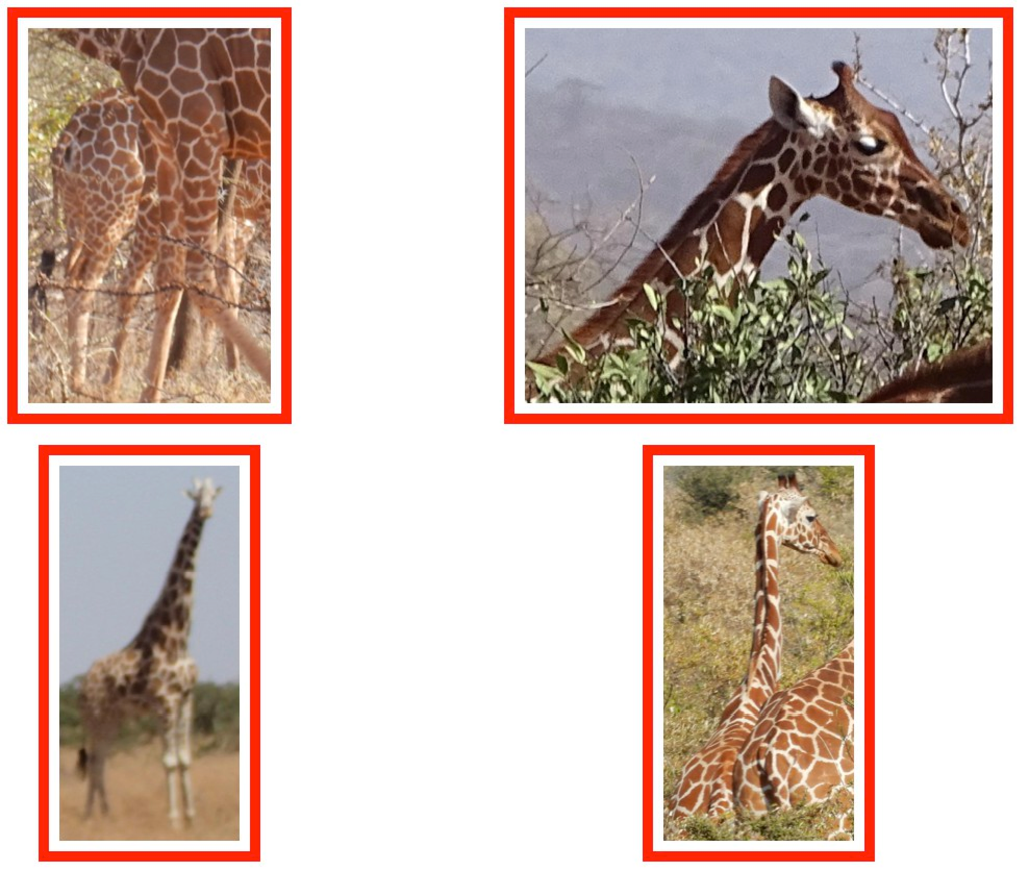
\includegraphics[width=0.45\linewidth]{resources/canonical-no-giraffe.pdf}
        \hspace{1mm}
        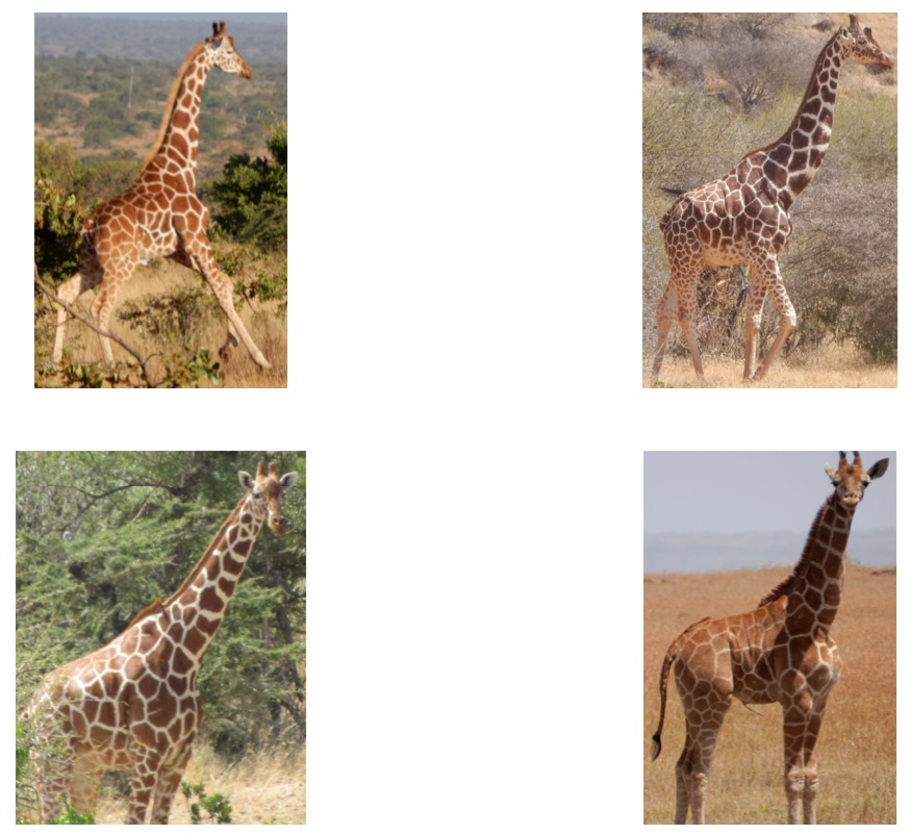
\includegraphics[width=0.45\linewidth]{resources/canonical-yes-giraffe.pdf}
    \end{center}
    \caption{Example images of Census Annotations for Gr\'evy's zebra and reticulated giraffe.  Annotations that were marked as non-CAs by a reviewer (left two columns) vs.\ marked as census (right two columns).  Gr\'evy's Zebra are displayed on the top two rows and reticulated giraffe are shown on the bottom two rows.}
    \label{fig:ca-census-zebra}
\end{figure}

\begin{figure}[!t]
    \begin{center}
        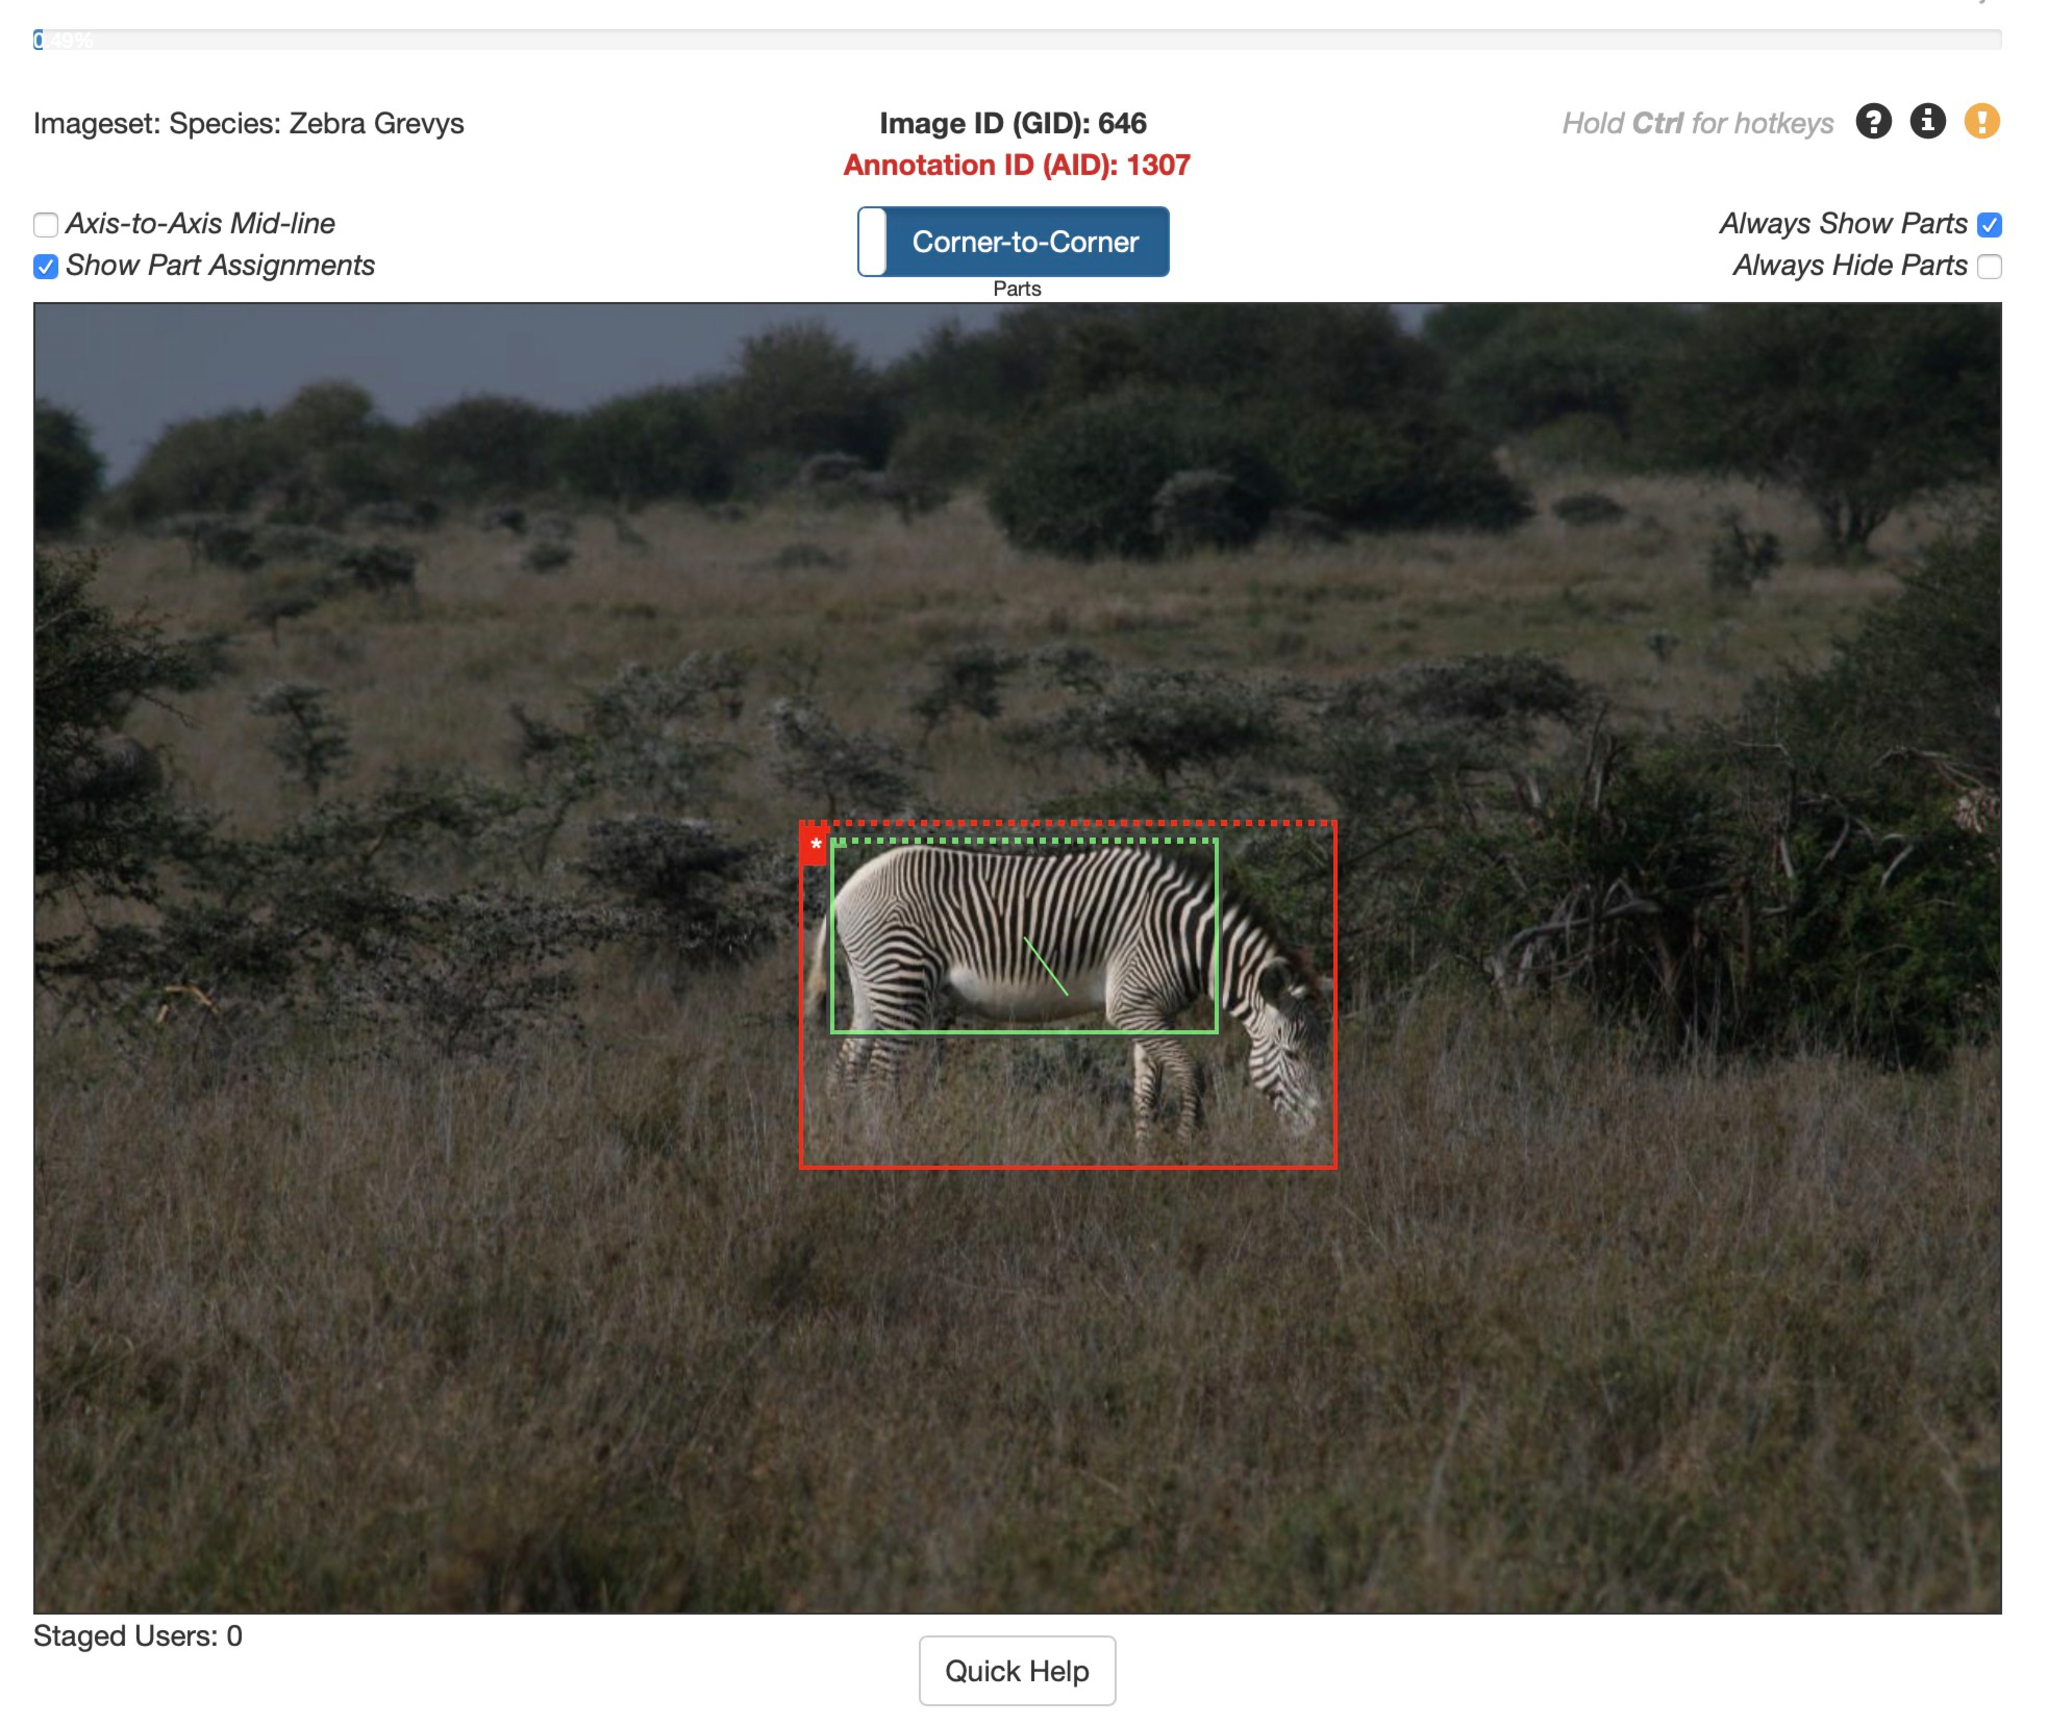
\includegraphics[width=0.70\linewidth]{resources/ca-ui-example.pdf}
    \end{center}
    \caption{An image of the Census Annotation Region web annotation interface.  The web interface used to annotate Census Annotation Regions (green box) onto existing Census Annotations (red box).  CA Regions are assigned to an existing annotation as a ``part'' and can inherit important metadata like species, viewpoint, and name assignments.}
    \label{fig:ca-interface}
\end{figure}

\begin{figure}[!t]
    \begin{center}
        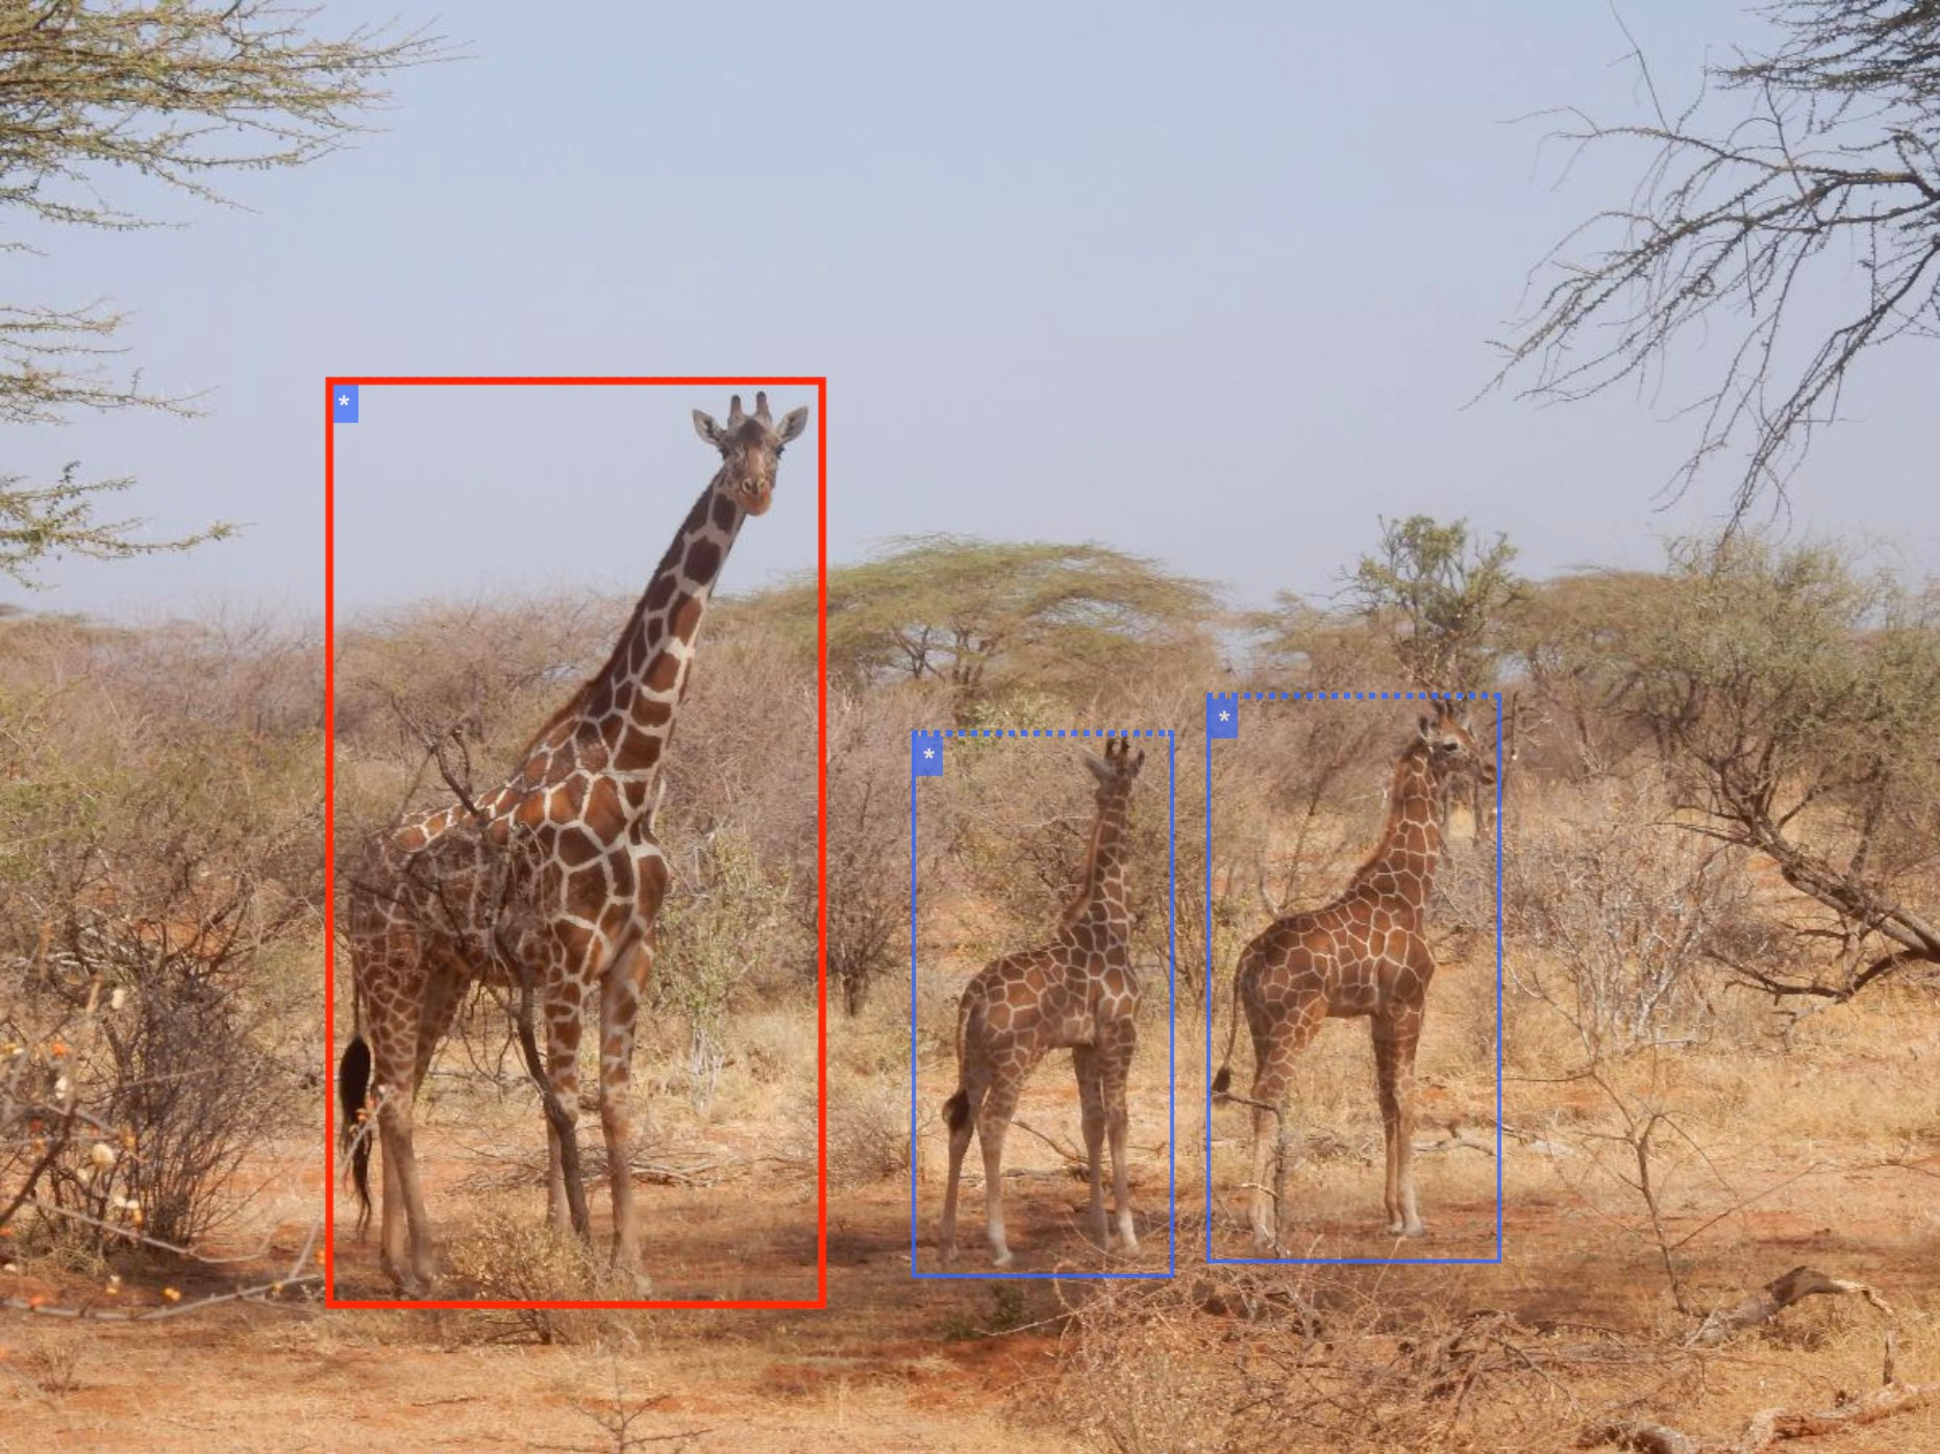
\includegraphics[width=0.45\linewidth]{resources/is_aoi_no_ca_image.pdf}
        \hspace{1mm}
        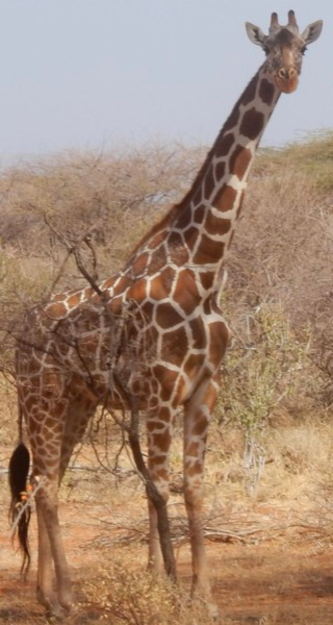
\includegraphics[width=0.18\linewidth]{resources/is_aoi_no_ca_annot.pdf}
        \\
        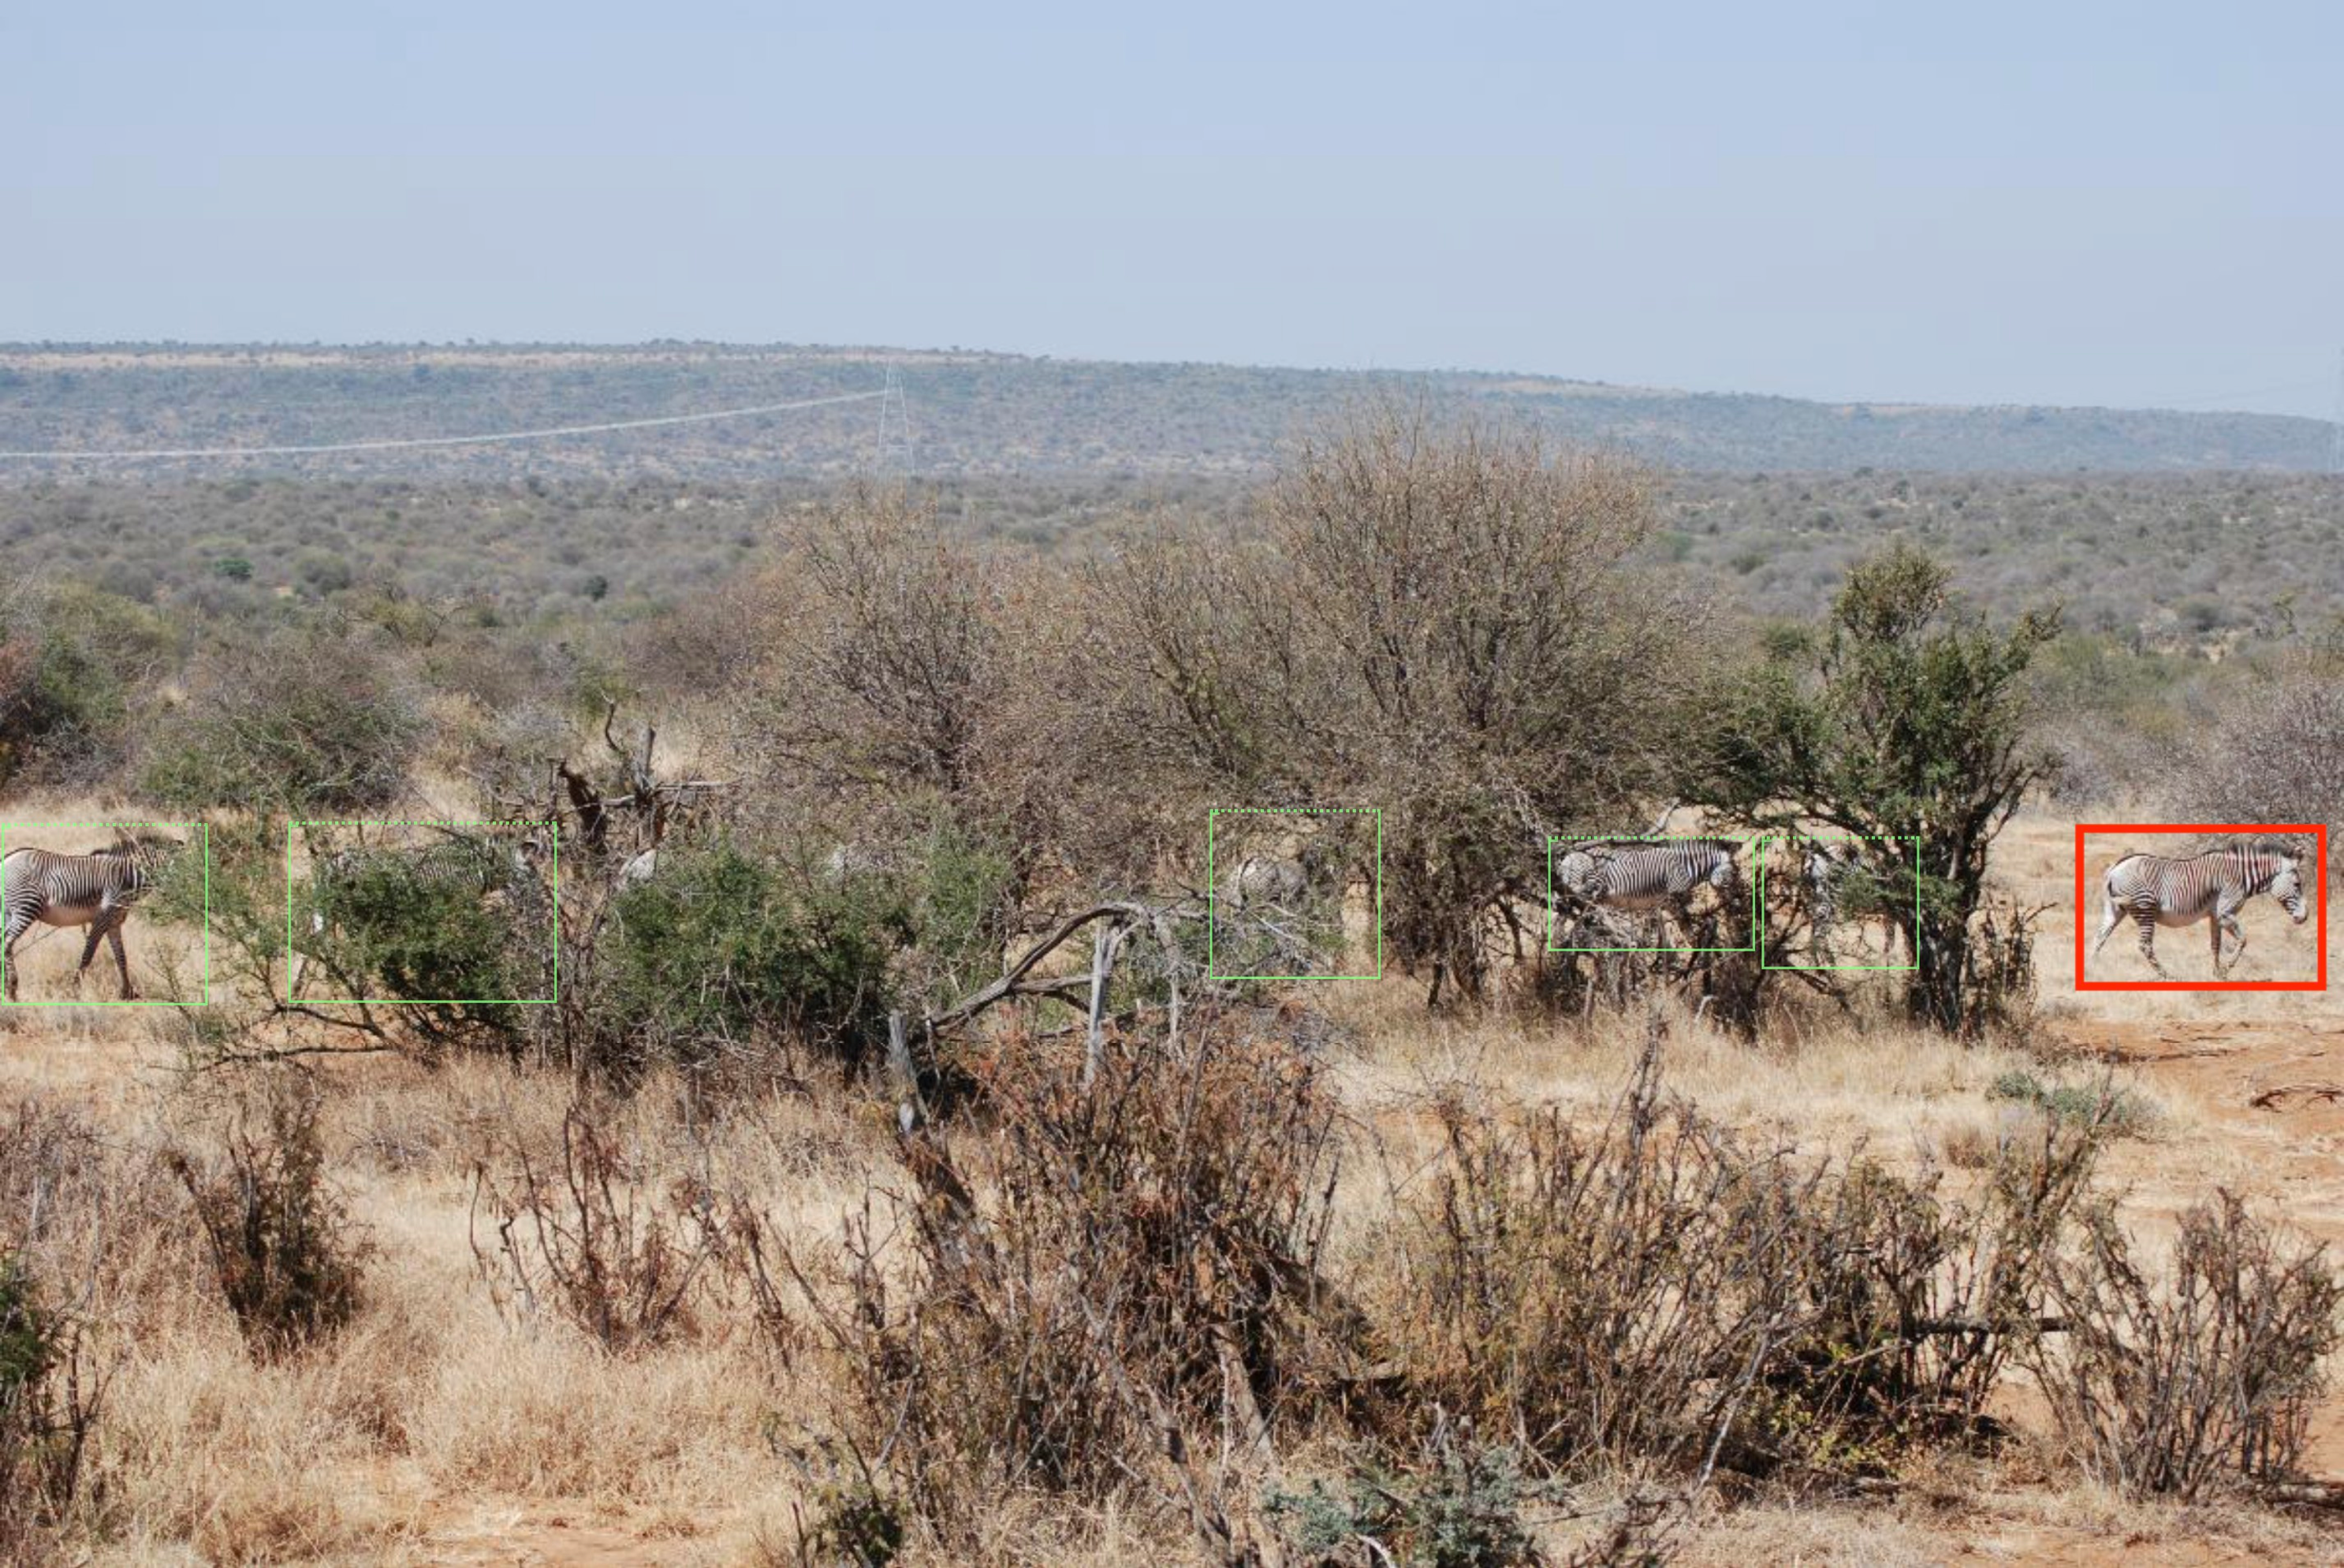
\includegraphics[width=0.45\linewidth]{resources/no_aoi_is_ca_image.pdf}
        \hspace{1mm}
        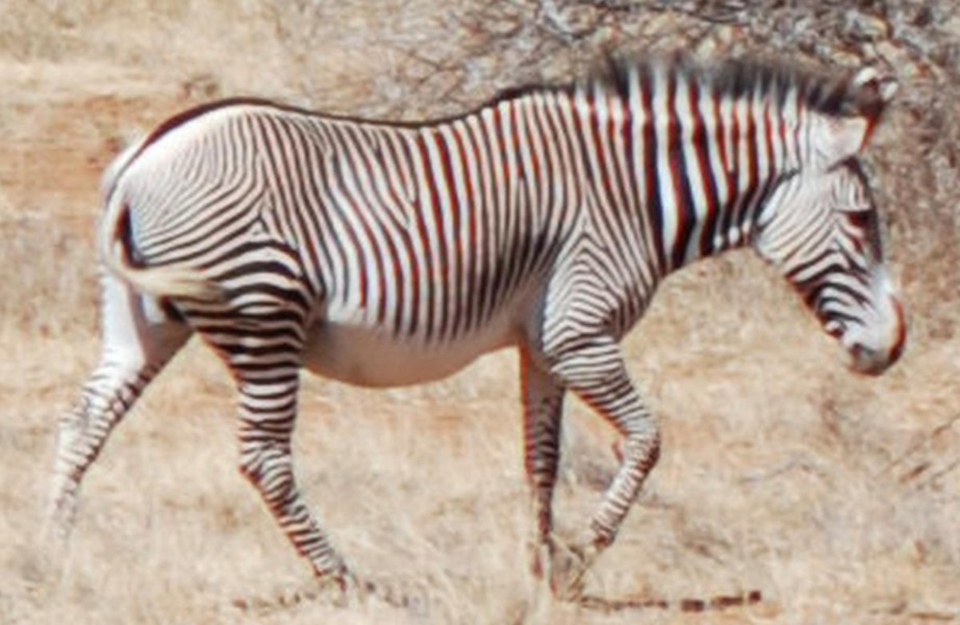
\includegraphics[width=0.45\linewidth]{resources/no_aoi_is_ca_annot.pdf}
    \end{center}
    \caption{Example images of the disagreement between AoI and Census Annotation.  The top row provides an example of an annotation that is an AoI but not a CA, with the annotation (left) and image (right).  The red annotations in the images are provided at a higher resolution to the right.  The giraffe is a borderline AoI due to its occlusion, but it is one of the primary subjects of the image and is decidedly in the foreground.  The bottom row gives an example of a Census Annotation that is not an AoI.  The animal is clearly comparable as seen by the annotation but is seen far away (small scale) and is a member of a herd, two items that make it a difficult case for AoI.}
    \label{fig:ca-comparison-aoi-ca}
\end{figure}

In total, the manual ground-truth labeling resulted in 1,837 Census Annotations (17.95\%) for Gr\'evy's zebra and 230 (9.9\%) for reticulated giraffe.  Figure~\ref{fig:ca-census-zebra} shows examples of Census Annotations (right, no border) and non-CAs (left, red border) for Gr\'evy's zebra (top two rows) and reticulated giraffe (bottom two rows).  All of the Census Annotations for Gr\'evy's zebra were then reviewed further with a different web interface (see Figure~\ref{fig:ca-interface}) to add Census Annotation Region bounding boxes.  The CA-R bounding box (green box) was required to be axis-aligned with the CA's bounding box (red box) and was not allowed to extend outside the bounds of the original CA annotation's bounding box.  In total, 1,837 boxes were annotated, one CA-R for each Gr\'evy's zebra CA in the training dataset.  The reticulated giraffe CAs were not annotated with CA-R boxes because of the relatively low number of examples for training and validation, with less than 50 annotations reserved for held-out experiments.  The images in the dataset were then partitioned into separate train (80\%) and validation (20\%) sets and stratified such that a balanced number of annotations per image occurred in each set.

\subsection{Comparison to Annotation of Interest (AoI) and Quality} \label{sec:ca-aoi-compare}

The concept of Census Annotation can be viewed as the annotation-level complement to Annotation of Interest (AoI).  The notion of an ``annotation of interest'' is inherently an image-level determination on the primary subject(s) of an image and functions to determine which animals were incidentally seen in the background.  This focus on finding good quality foreground sightings of animals is related to Census Annotation, but AoI and CA do not overlap perfectly in their goals.  In contrast, Census Annotation represents the comparability between two annotations.  The notion of CA ensures that reliable identifying information is always available, regardless of where and how the annotation exists in the image composition.  Figure~\ref{fig:ca-comparison-aoi-ca} provides examples of when AoI and CA can disagree.  While an annotation that is not an AoI is also not likely to be a Census Annotation, it is not guaranteed to be the case, as seen in the bottom row.  An annotation can also be considered an AoI based on the semantic context of the image but does not show enough clear and reliable ID information to be considered a Census Annotation (top row).

Furthermore, the detection pipeline's labeler has the ability to predict an explicit ``quality'' value for annotations (e.g. \textit{junk}, \textit{good}, \textit{perfect}).  This feature was originally used in previous experiments with photographic censusing (see~\cite{parham_photographic_2015}) to filter annotations for ID curation but was ultimately abandoned.  The problem is that ``quality'' is a fairly subjective measurement (i.e., it is hard to get consistent ground-truth labels) and does not guarantee that two acceptable quality annotations will be comparable.  Although a quality metric and AoI can be highly correlated with Census Annotation, they are insufficient replacements when the goal is to eliminate incomparable decisions from ID curation.  As such, the eventual formulation of Census Annotation is the culmination of real-world experimentation with large censusing events that have failed to achieve high degrees of automation (due to challenges discussed previously in Chapter~\ref{chapter:overview}).

The notions of AoI, quality, and CA can be compared and contrasted using the ground-truth labels in the GZCD.  In that dataset, there is a total of 9,205 Gr\'evy's zebra annotations.  Of those, 4,246 have been ground-truth annotated as AoIs, 7,372 show some degree of the animal's right side, and 4,119 have an acceptable quality value. In addition, there are 4,005 Census Annotations in that dataset, with a 93.4\% overlap with a quality filter and 87.4\% overlap with AoI.  In summary, these values suggest that a quality metric and even AoI can be somewhat helpful in filtering annotations, but with the addition of CA to the detection pipeline, they are largely redundant.  That being said, Annotation of Interest is still used to validate the detector's performance and is still worthwhile to annotate, but a quality value for each annotation is no longer necessary as Census Annotation has superseded it.  We will now shift our attention to the implementation details of the CA and CA-R methodologies and analyze their stand-alone performances as new detection components.

\section{Census Annotation (CA)} \label{sec:ca}

\begin{figure}[!t]
    \begin{center}
        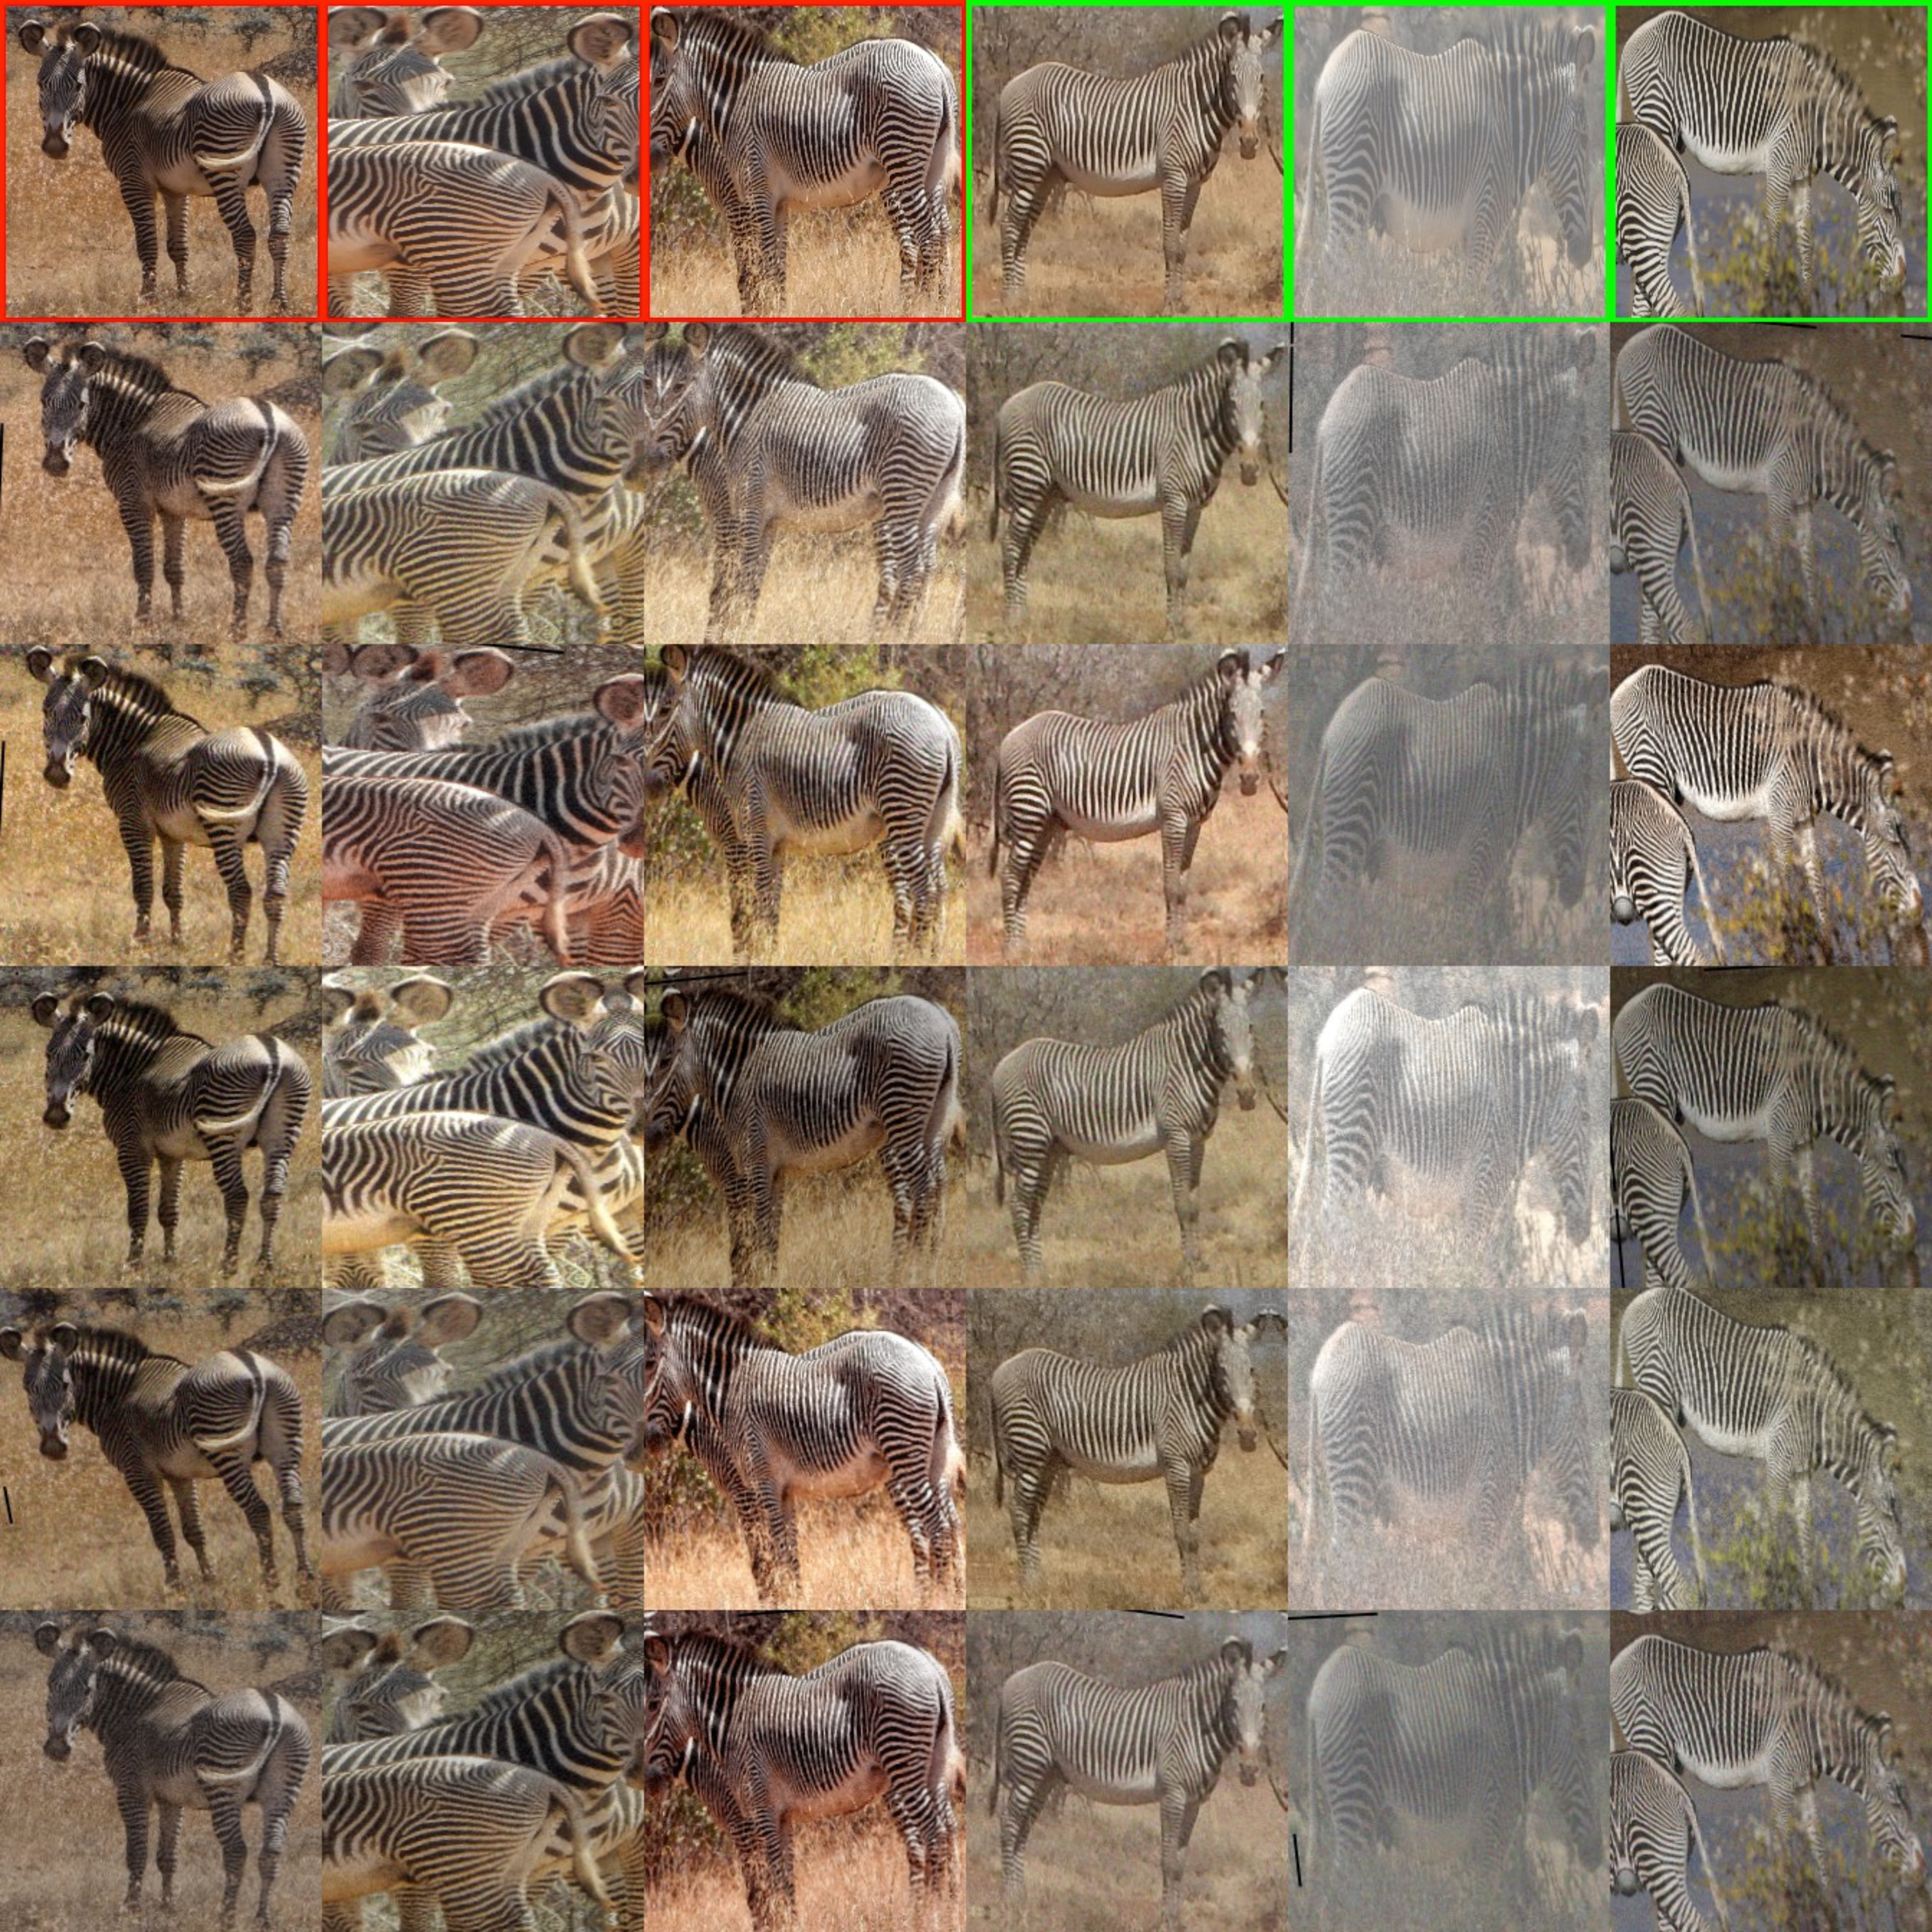
\includegraphics[width=0.70\linewidth]{resources/ca-augment.pdf}
    \end{center}
    \caption{Examples of on-the-fly training augmentations for the Census Annotation classifier.  Positive samples are highlighted with a green border (CA examples) while negative samples have a red border (Non-CA examples).  Each example received a unique, randomized augmentation for each epoch and was computed on-the-fly.}
    \label{fig:ca-augmentation}
\end{figure}

The Census Annotation classifier was trained using a pre-trained DenseNet 201~\cite{iandola_densenet:_2014} feature extraction network with a linear classification layer added on top.  The network was fine-tuned with SGD (LR 0.001, momentum 0.9, and a ten epoch patience LR schedule) and used a standard Cross-Entropy loss.  The input images were sent through a moderate level of data augmentation (e.g., contrast normalization, per-channel pixel noise, hue and saturation changes, piece-wise Affine transformations on a small grid, and slight rotations and shearing).  Example augmentations for a given image (top row) can be seen in Figure~\ref{fig:ca-augmentation} for negative non-CA (red border) and positive CA (green border) annotations.  Furthermore, each mini-batch was sampled such that it had a balanced number of positive and negative examples.  The classifier was trained as an ensemble of three separate neural network models (each with unique initialization), and their respective outputs are averaged into a single prediction during inference.  This neural network design is standardized and shares principles with existing detection pipeline classification components like the annotation labeler (see Section~\ref{sec:labeler}).  The CA component remains independent of previous detection methods, however, and its modular implementation can be disabled or updated as needed without impacting other components.

\begin{figure}[!t]
    \begin{center}
        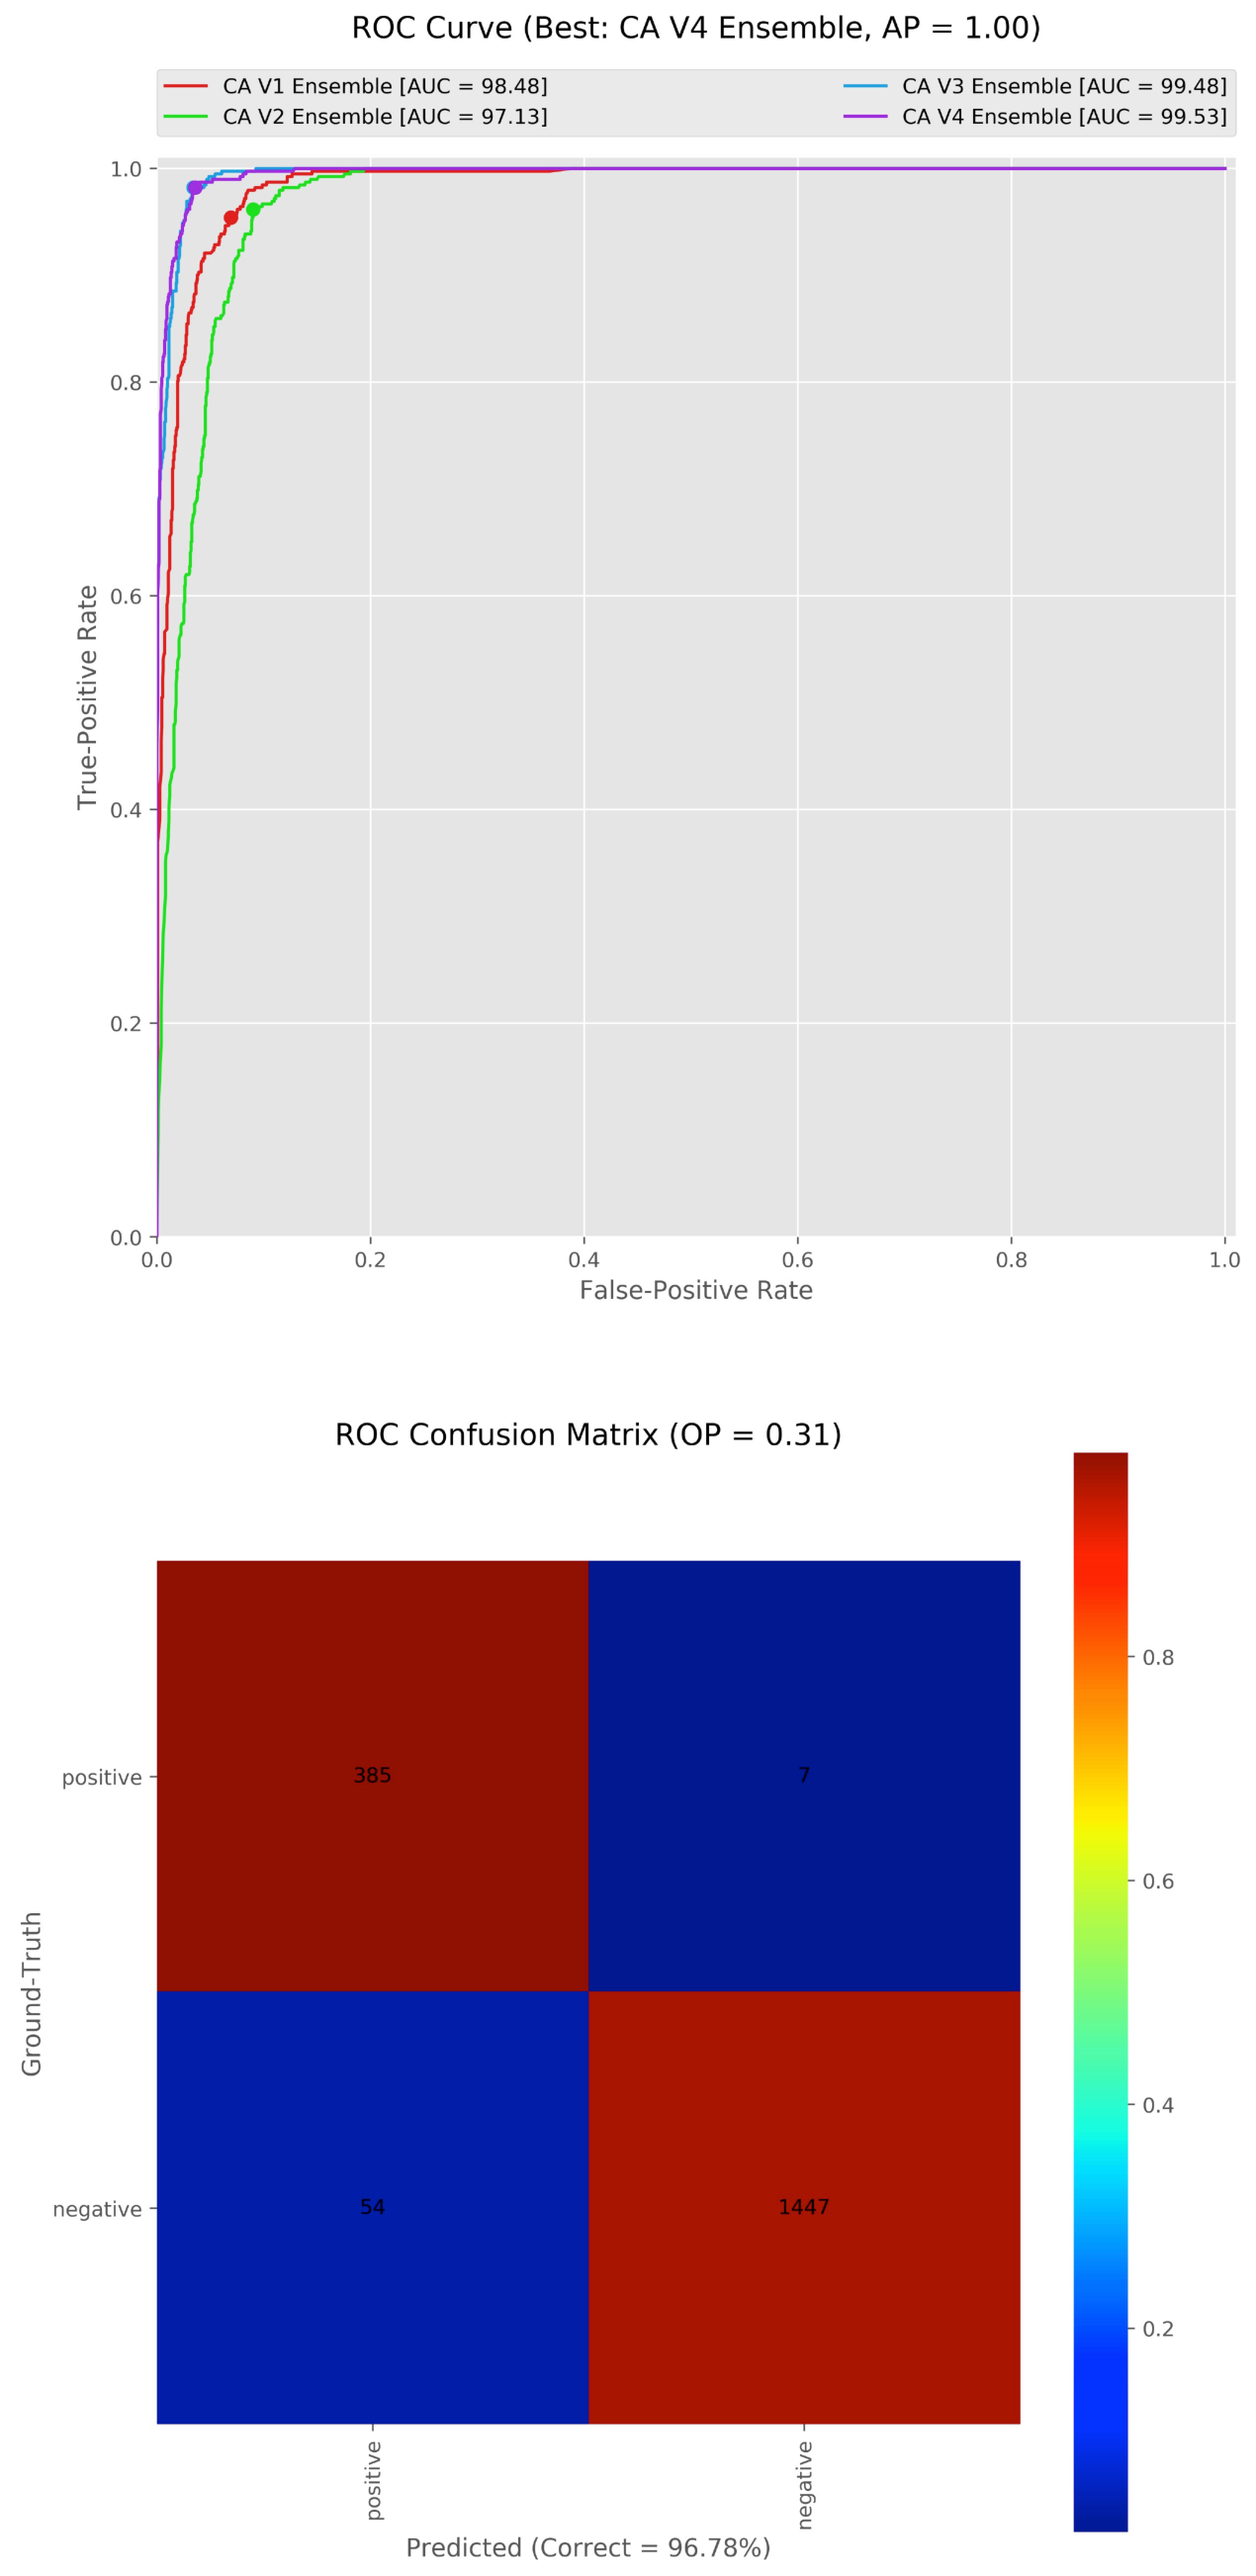
\includegraphics[width=0.48\linewidth]{resources/ca-census-classifier.pdf}
        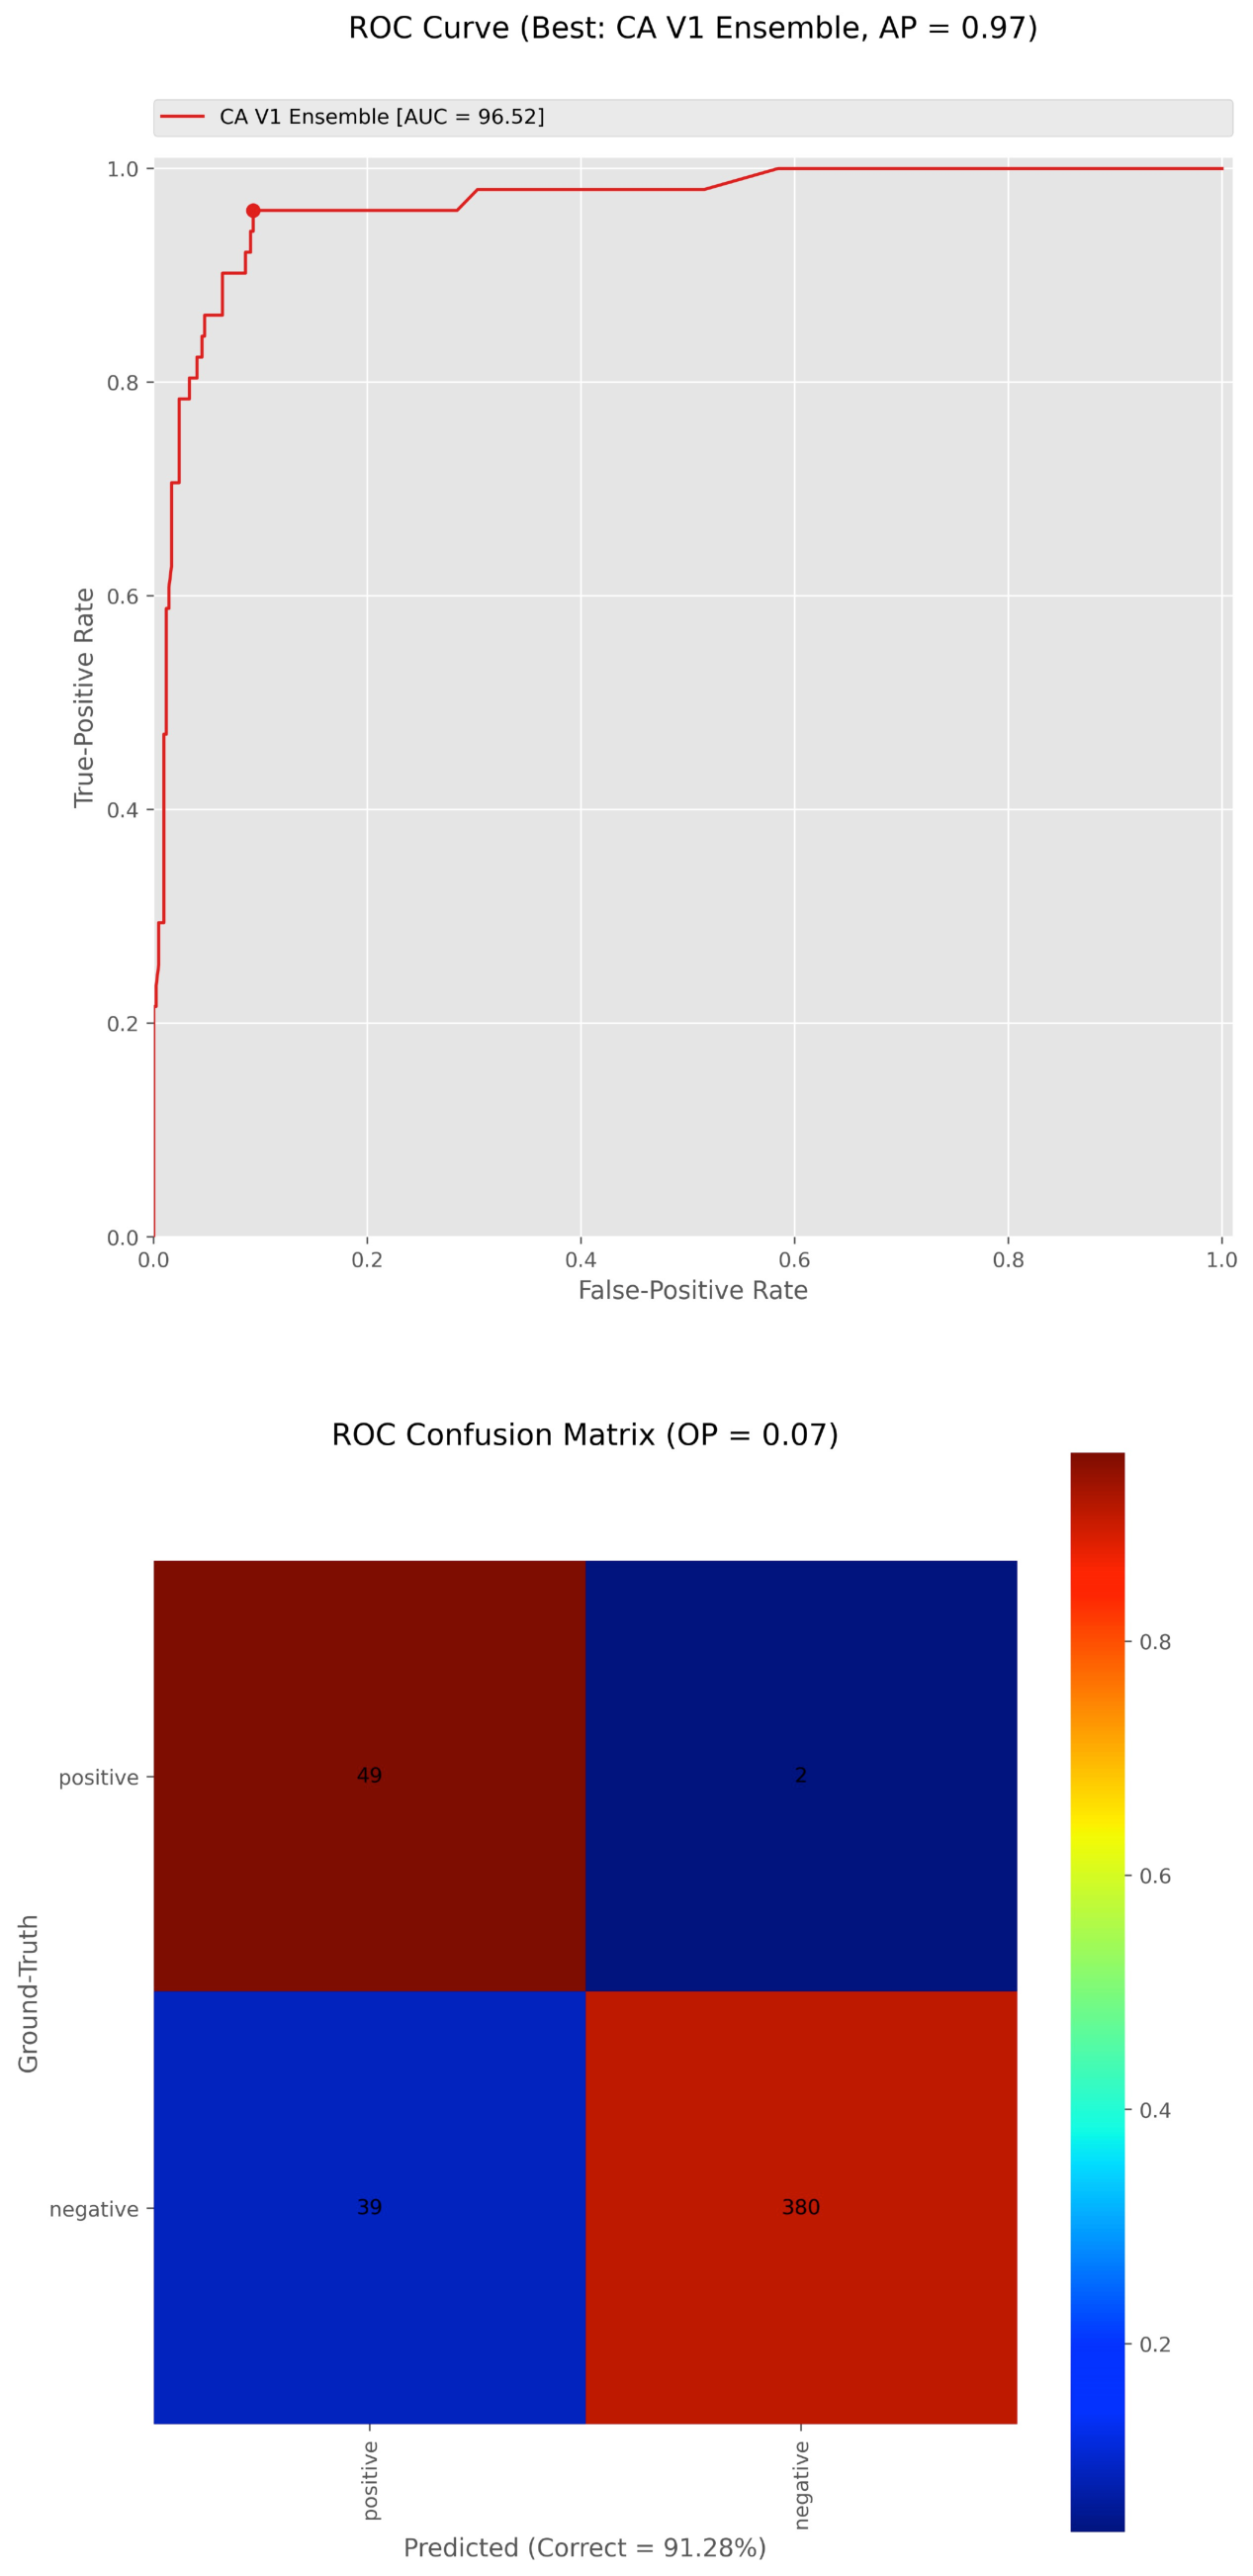
\includegraphics[width=0.48\linewidth]{resources/canonical-precision-recall-roc-giraffe.pdf}
    \end{center}
    \caption{The ROC performance curves for the Census Annotation classifier.  Top: ROC curves showing the classification performance and their respective Area-Under-Curve volumes (AUC) for Gr\'evy's zebra (left) and reticulated giraffe (right).  Bottom: The Confusion Matrix for the best model (V4 for zebras, V1 for giraffe) and best operating point (zebra OP=0.31, giraffe OP=0.07) as determined by the colored dot in the various ROC curves.  The accuracy of the Gr\'evy's zebra CA classifier is 96.8\% and 91.3\% for reticulated giraffes, but if false positives are treated as extra work and not errors then the accuracy increases to 99.6\% for both models.}
    \label{fig:ca-census_classifier}
\end{figure}

A series of four CA classifier models were trained using different configurations of data augmentation and iteratively better ground-truth training data between each version.  The training examples for each CA classifier were selected using a simple species filter and did not consider viewpoint or quality.  The purpose was to train the CA models on ideal CA examples, annotations that were obviously incorrect (e.g., wrong viewpoint), and annotations that had relatively good quality overall but were ultimately incomparable.  The final version (V4) has the best performance on the held-out validation data (see Figure~\ref{fig:ca-census_classifier}, left). This result is expected as the data augmentation scheme was improved for that model to be more aggressive (acting as a better regularizer). In addition, it was trained on the cleanest data after label corrections were applied to the ground-truth.  In total, 26 CA ground-truth labeling errors (0.6\%) were identified in the GZCD and fixed by hand.  Overall, the V4 model achieves a classification accuracy of 96.8\% for Gr\'evy's zebra using an operating point (OP) of 0.31. In addition, the model makes 54 false positive (FP) decisions compared to 7 false negatives (FN).  This balance of errors is a good trade-off for a filtering component because we can treat Type I misclassifications as extra work (and not invalid data) during ID curation.  Therefore, the practical success rate of the classifier is 99.6\% when we consider false negatives are the most problematic source of error.

The Census Annotation classifier was also trained and evaluated on reticulated giraffes.  Even though the total number of annotations was significantly smaller, the CA classifier still did well to classify 91.3\% of the examples correctly (see Figure~\ref{fig:ca-census_classifier}, right).  Suppose we apply the same logic about false positives being a less worrisome type of error. In that case, the model only makes two mistakes out of 470 annotations (99.6\%) on held-out validation data for the price of reviewing an additional 39 annotations.  Upon inspection, the annotations that the zebra and giraffe models incorrectly predict as CAs are mostly borderline (subjective) cases in the ground-truth labels.  Ultimately, the number of giraffe annotations in the GZCD was too small for a worthwhile evaluation with CA-R.  Moreover, the GZCD focused exclusively on Gr\'evy's zebra, so a large, authoritative ID dataset does not currently exist to demonstrate any potential improvements in incidental matching.  The lack of a reliable ID database for reticulated giraffes is primarily due to limited resources considering how much time and energy was spent curating and verifying the Gr\'evy's zebra IDs in the GZCD.  As such, the remaining analysis on CA-R, and following discussions in this chapter, are focused entirely on Gr\'evy's zebras.

\section{Census Annotation Region (CA-R)}

\begin{figure}[!t]
    \begin{center}
        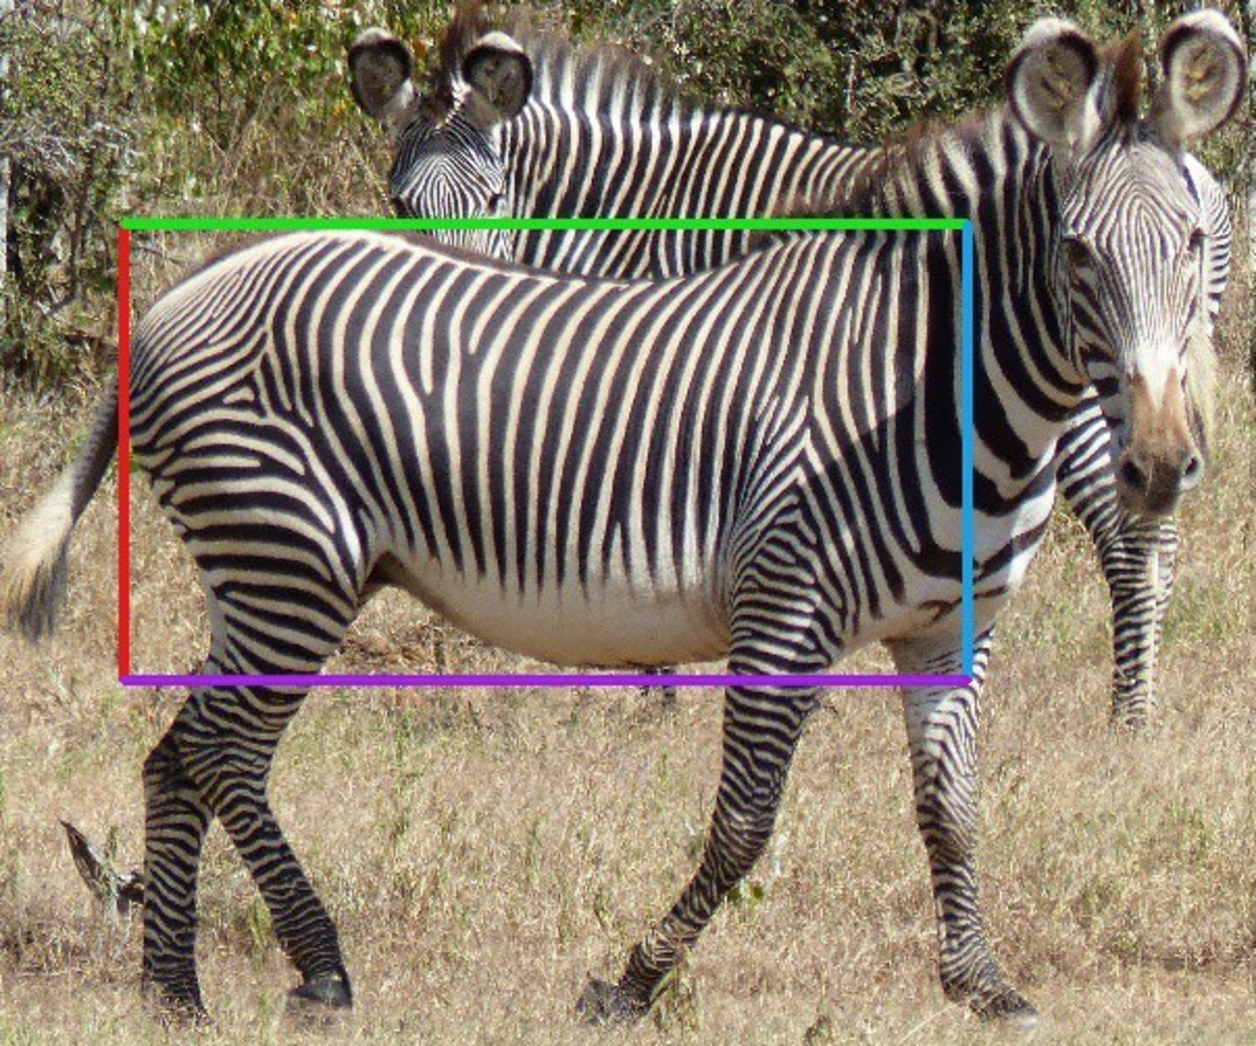
\includegraphics[width=0.70\linewidth]{resources/ca-canonical-regression-iou-68-aid-4651.pdf}
    \end{center}
    \caption{An example image of a Census Annotation Region, which is defined by its four edge components: \texttt{x0} (left, red), \texttt{x1} (right, blue), \texttt{y0} (top, green), and \texttt{y1} (bottom, purple).}
    \label{fig:ca-edges}
\end{figure}

The Census Annotation Region model was trained as a regression network that is tasked with predicting four simple values (shown in Figure~\ref{fig:ca-edges}): \texttt{x0} (left, red), \texttt{x1} (right, blue), \texttt{y0} (top, green), and \texttt{y1} (bottom, purple).  All of the original CA bounding boxes are assumed to be rotated where the animal's head is at the top of the box.  Furthermore, the CA Region bounding boxes were all assumed to have inherited the rotation of their associated CA.  This setup means that each of the four edges of the CA Region bounding box (top, bottom, left, and right) can be represented by a single value for how many pixels it is away from the corresponding edge of the CA's bounding box.  All x-axis pixel offsets are converted to a decimal value from 0.0 to 1.0 by dividing by the annotation's width.  This process is repeated for y-axis pixel offsets with the pixel height of the annotation.  Therefore, the network was trained to predict a positive value between 0.0 and 1.0 for each of the four edges of the CA Region's bounding box as a residual from the original box's bounding box location.

The CA-R regression network has a similar convolutional back-end to the CA classifier: the model is fine-tuned with SGD (initial LR 0.0005), uses similar data augmentation as the CA model (but without translation or rotation operations), has a DenseNet 201 architecture with pre-trained weights, and uses a 4-node linear layer for its output.  The network is optimized using a modified loss function for mean squared error (L2), with additional terms for the ``over-shooting'' ($\alpha$) and ``under-shooting'' ($\beta$) components of the standardized regression loss.  In general, the expectation is that any distracting background information is along the edge of the CA's original bounding box.  We are trying to minimize background information, but that goal should not come at the cost of accidentally removing useful ID information on the animal's body.  The resulting loss term is defined as:

\begin{align}
    \begin{split}
        \text{Loss}_{\text{CA-R}} &= \sum_{n=1}^{n} \sum_{c=1}^{4} \alpha * (\text{min}(0, x_{n,c} - \bar{x}_{n,c}))^2 + \beta * (\text{min}(0, \bar{x}_{n,c} - x_{n,c}))^2
    \end{split}
\end{align}

\noindent where $x_{n,c}$ is the ground-truth value, $\bar{x}_{n,c}$ is the predicted value by the network, and $c$ represents the four possible axes.  The CA-R regression models are also trained as an ensemble of three separate neural networks, and their final results are averaged during inference.

\begin{figure}[!t]
    \begin{center}
        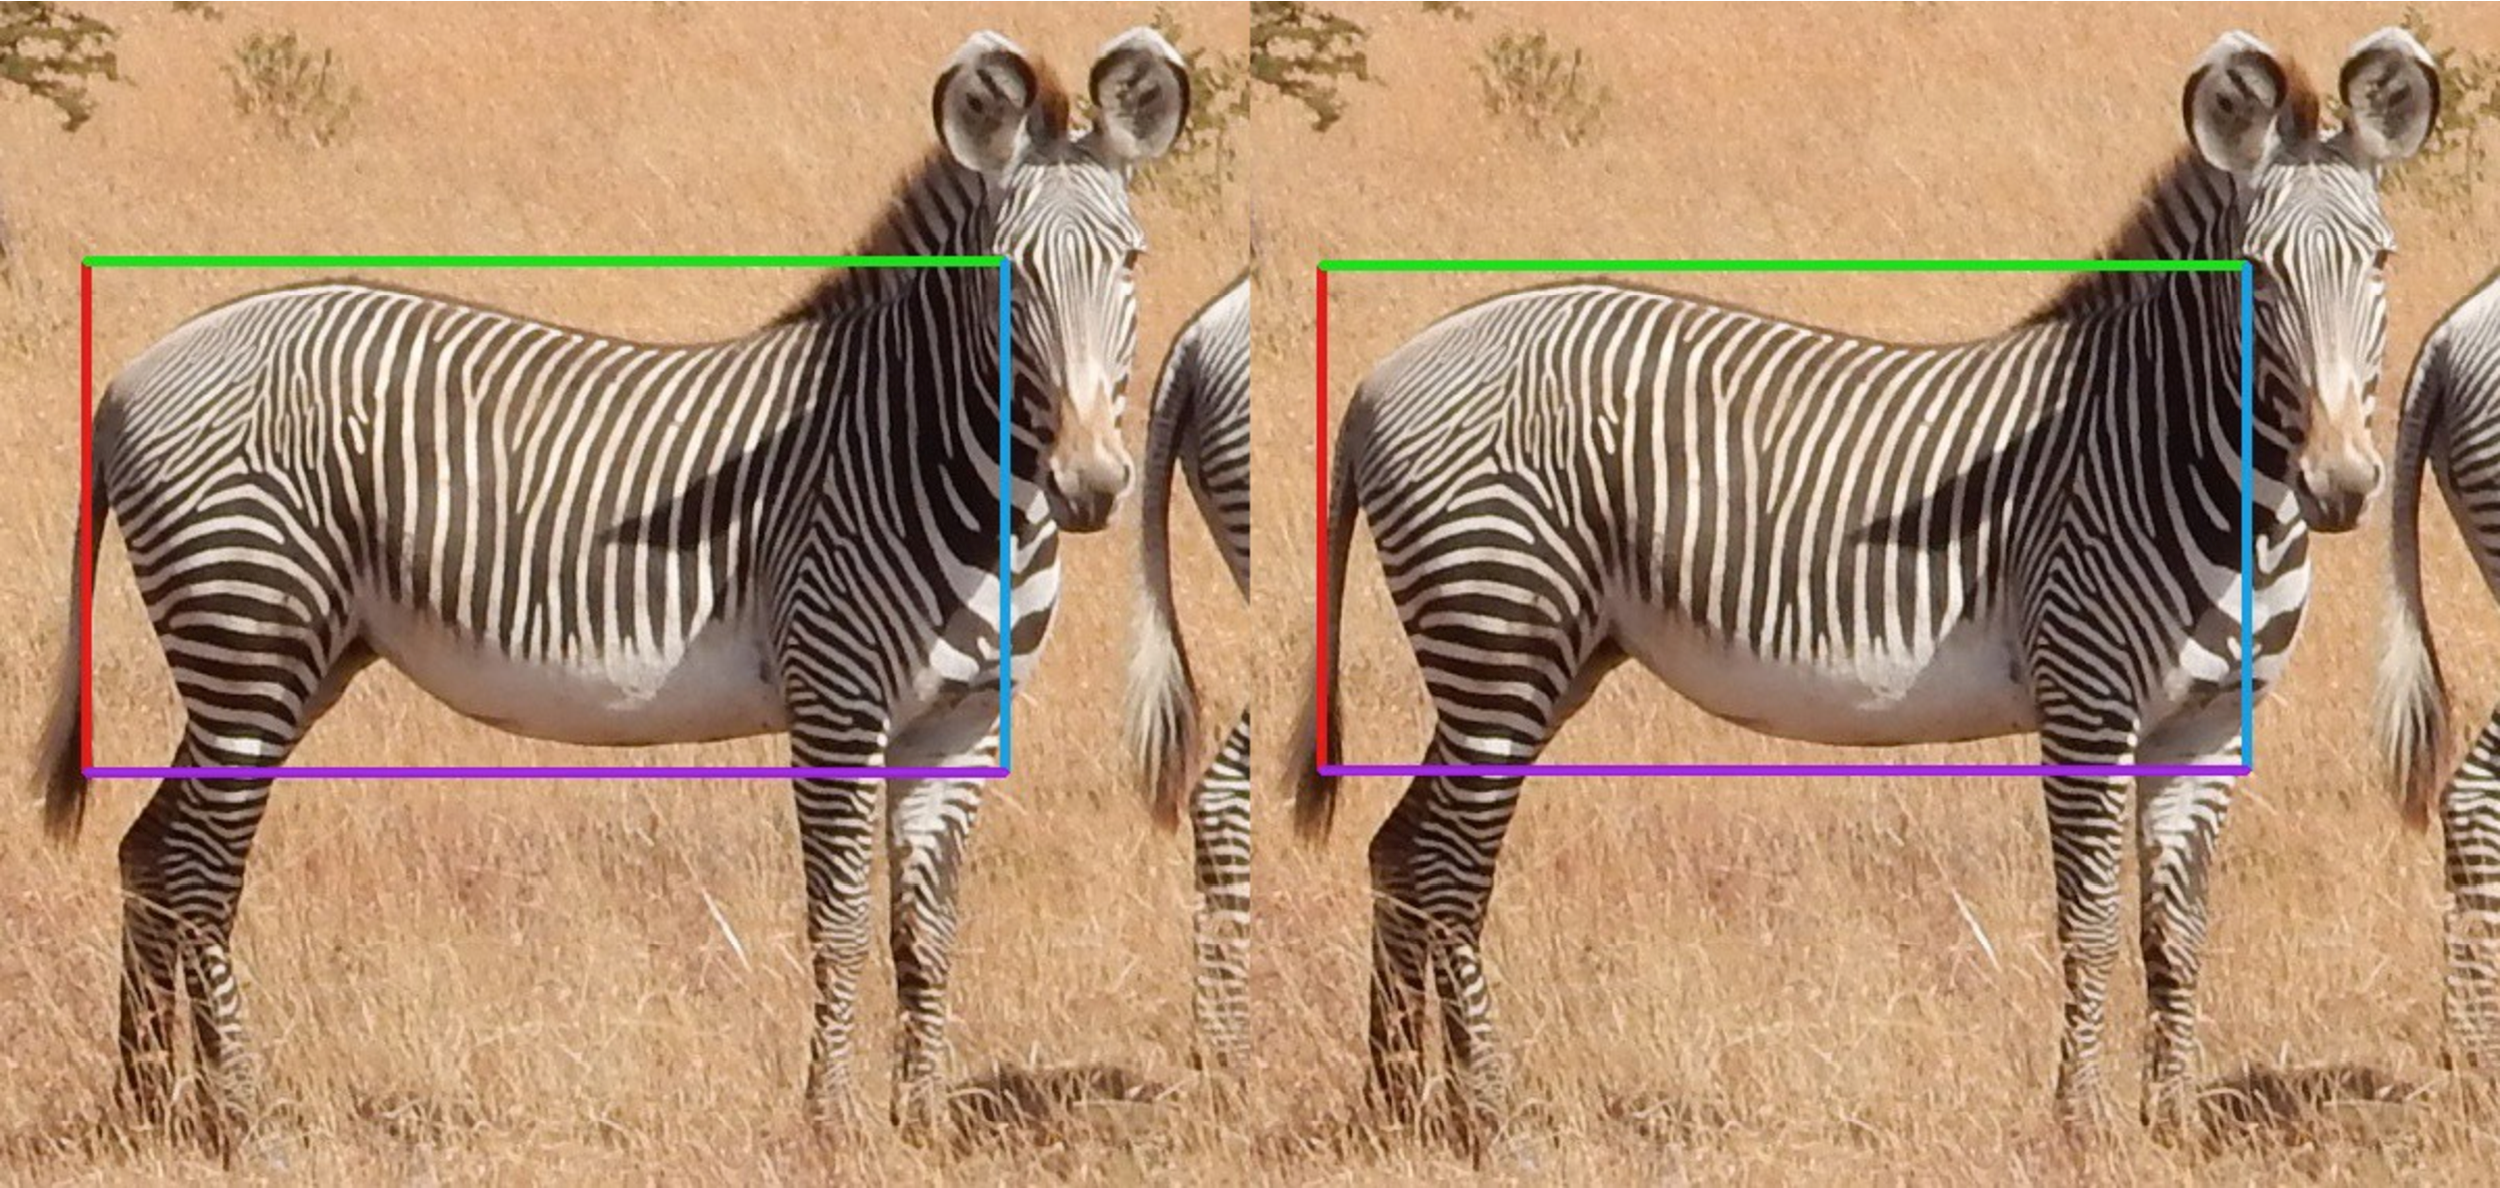
\includegraphics[width=0.70\linewidth]{resources/ca-canonical-regression-iou-96-aid-11470.pdf}
        \\
        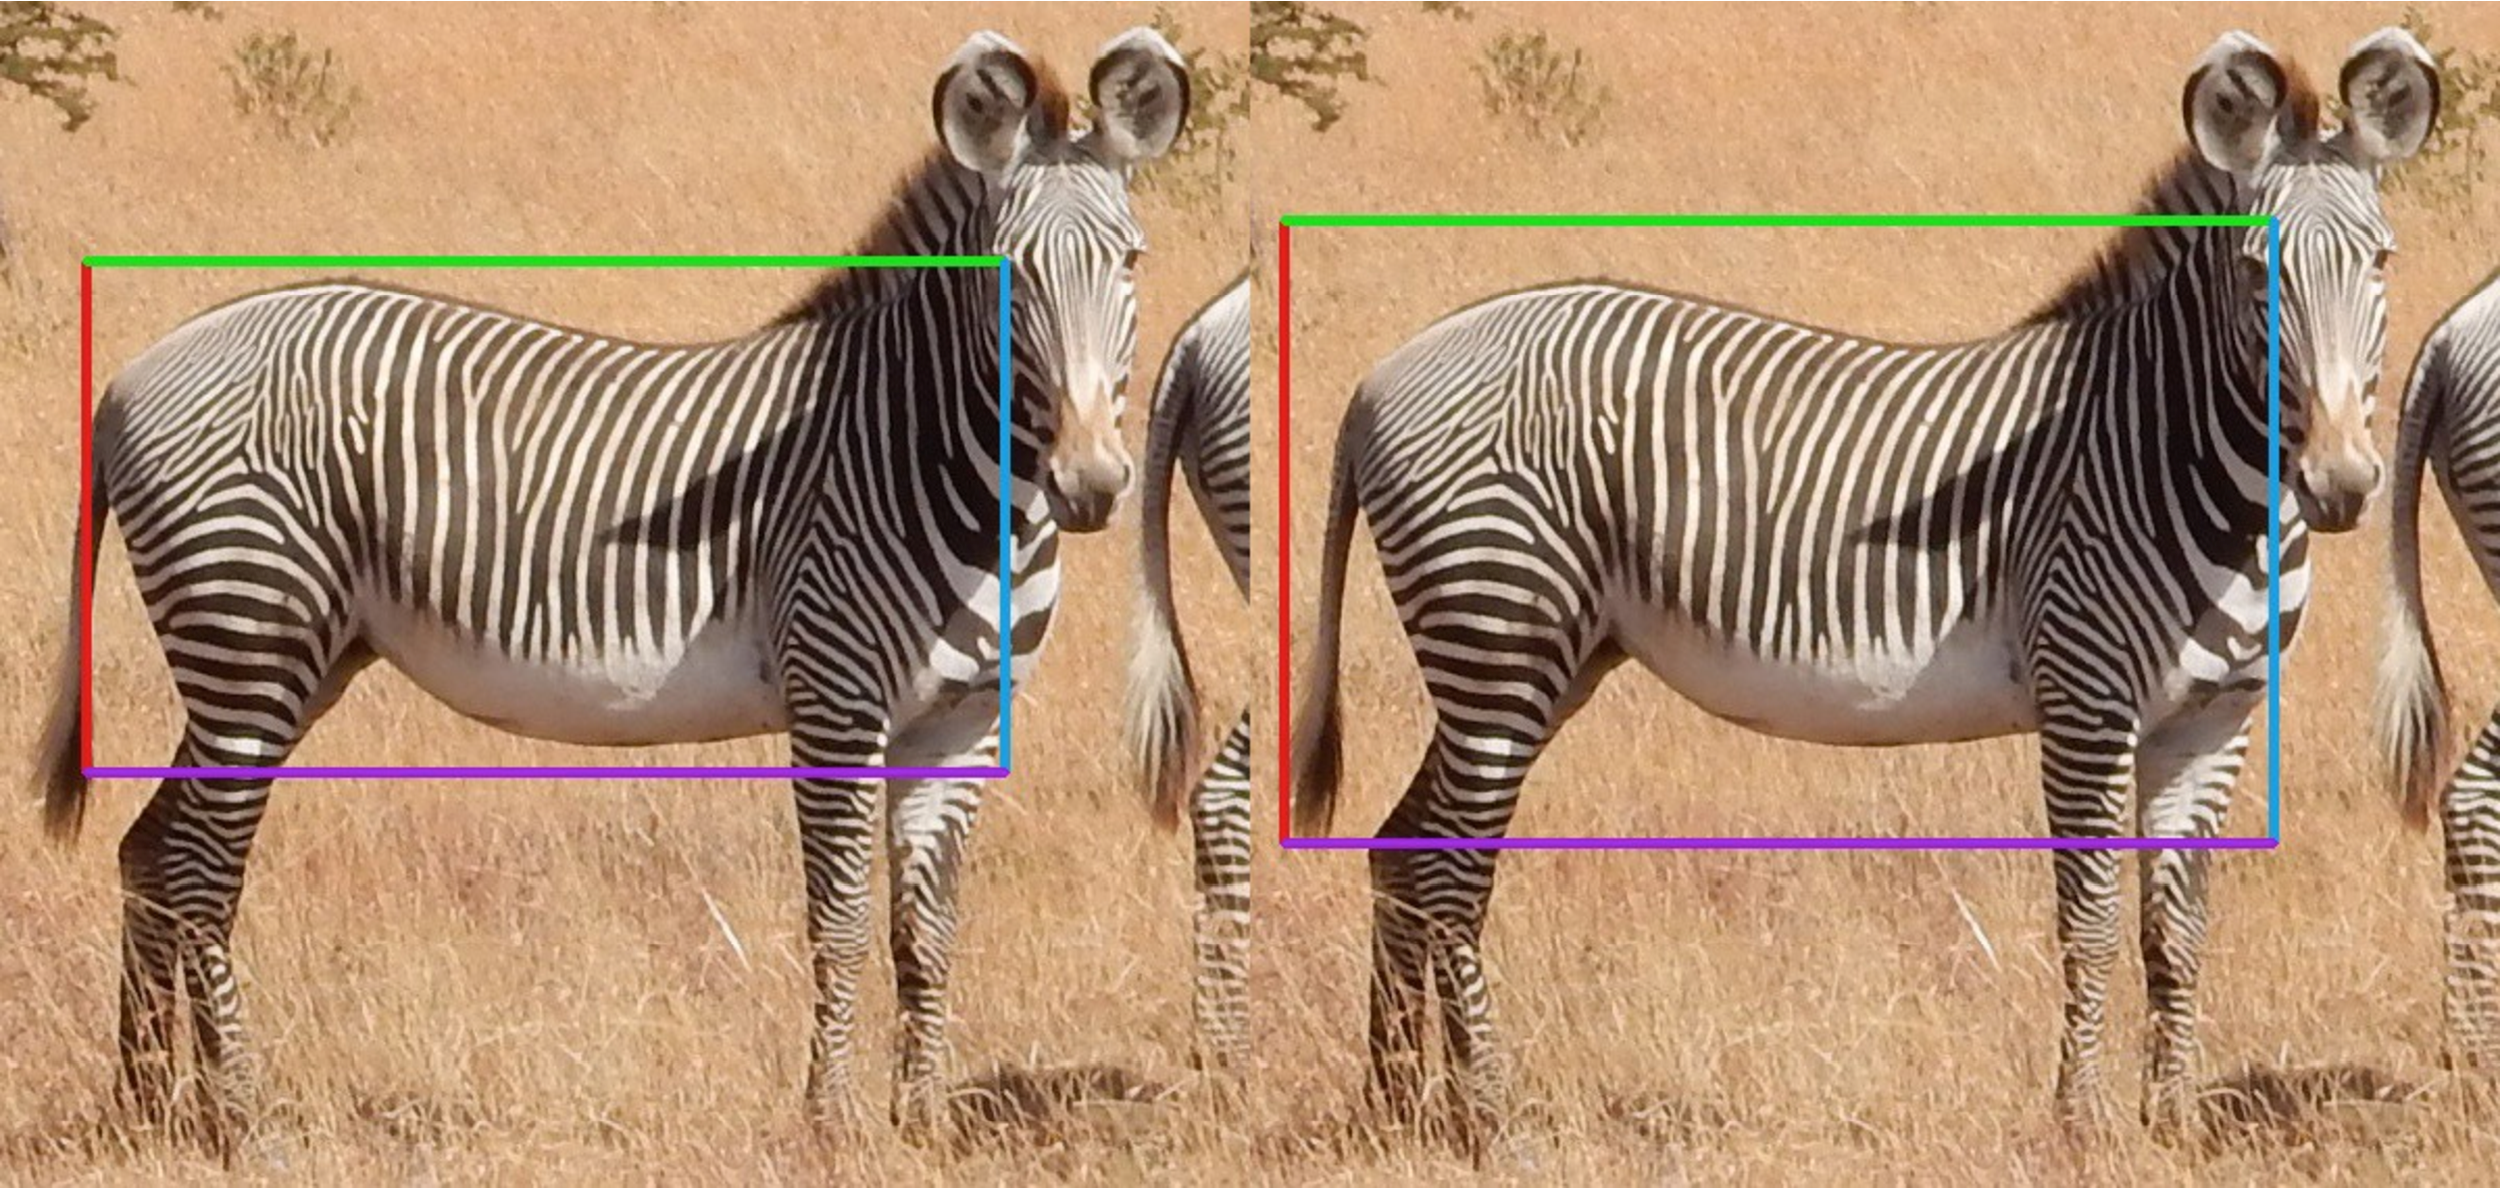
\includegraphics[width=0.70\linewidth]{resources/ca-canonical-regression-iou-76-aid-11470.pdf}
    \end{center}
    \caption{An example comparison of a Census Annotation Region output with different training configurations for overshooting.  The figure shows an example output (right column) for the CA Region model V6 (top row) vs.\ V4 (bottom row) for an input annotation (left column).  The input annotations to both models are identical.  Two networks are offered to precisely predict the box on the margin (V6) or prevent overshooting (V4).  We should prefer the larger predicted CA Region because it has less of a chance of throwing away useful information for ID.}
    \label{fig:ca-iou}
\end{figure}

\begin{figure*}[!t]
    \begin{center}
        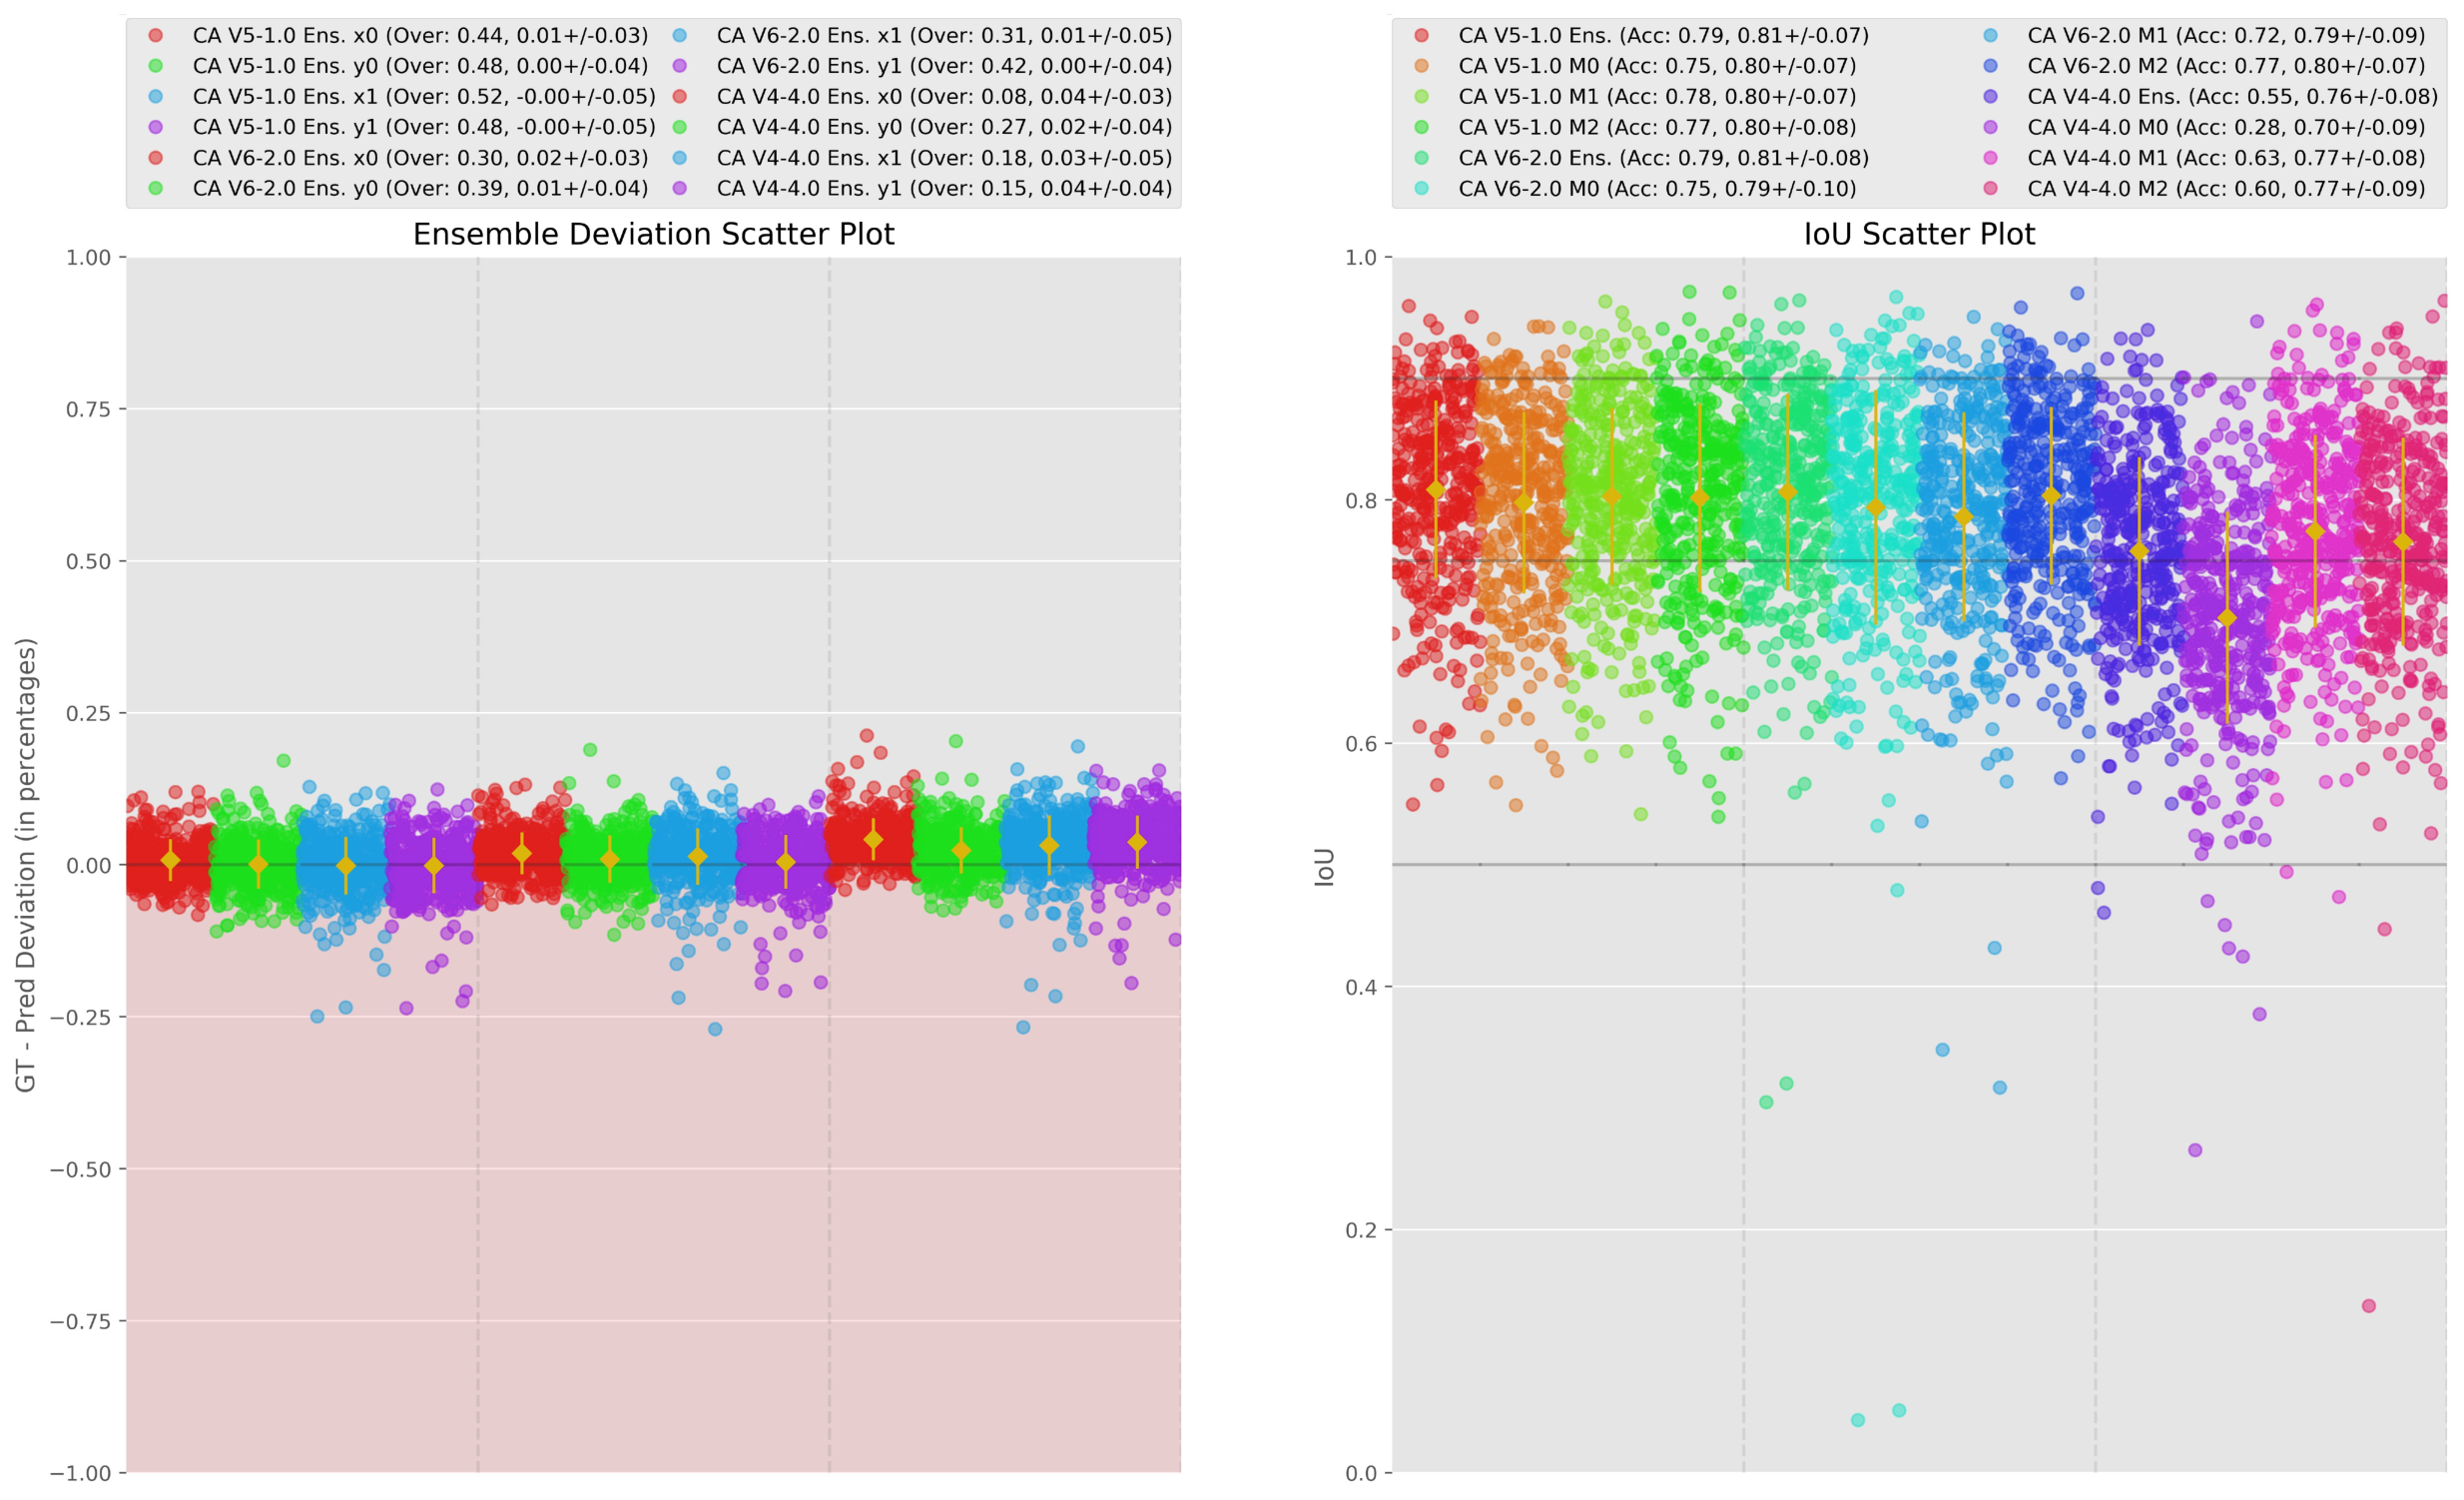
\includegraphics[width=0.90\linewidth]{resources/ca-census-regions.pdf}
    \end{center}
    \caption{The regression performance curves for the Census Annotation Region component.  Left: A deviation plot of each of the four edges for each of the three models.  Right: An Intersection-Over-Union (IoU) scatter plot showing how well the predicted CA Region overlaps with the ground-truth box.  An IoU greater than 0.5 is generally considered a correct detection with a value of 0.75 has a high degree of overlap.}
    \label{fig:ca-census_regression}
\end{figure*}

A series of six CA-R ensembles were trained, partially to help identify and correct ground-truth errors similar to the process used for the CA classifier.  The first three models (versions 1, 2, and 3) were used to bootstrap a better, cleaner dataset and were discarded after the issues they identified were fixed.  The next three models (versions 4, 5, and 6) are useful to compare as they are trained on the same underlying CA-R data.  When $\alpha$ and $\beta$ are both set to 1.0, the network's loss is exactly L2 and is expected to balance the errors from over-shooting against under-shooting equally.  This loss formulation is a problem, however, because it suggests that half of the predicted boxes will have edges that overshoot the target offset (making the CA-R box too small, cropping out useful ID information) and the other half will undershoot (making the box too large, increasing the likelihood of incidental matching).  Overall, the ideal CA-R model should be trained to eliminate as much under-shooting as possible while doing very little (if any) over-shooting.  The V4 model was trained with a 4:1 ratio (quadruple the loss penalty for over-shooting, $\alpha=4$, $\beta=1$), V5 with a ratio of 2:1 ($\alpha=2$, $\beta=1$), and the V6 model with a 1:1 ratio (L2 norm, $\alpha=1$, $\beta=1$).  By comparing the relative errors of each model configuration, the preferred behavior can be selected when creating CA-R bounding boxes.  Figure~\ref{fig:ca-iou} shows an example of what kinds of predicted boxes the V6 and V4 models generate.

Figure~\ref{fig:ca-census_regression} (left) shows that the 3 models do a very good job at approximating the values for \texttt{x0}, \texttt{x1}, \texttt{y0}, and \texttt{y1}.  In this plot, the values that are less than 0 on the y-axis are highlighted (in red), as this indicates a overshoot of the prediction.  While the V6 predictions are mean centered at 0.0 (or 1\% for \texttt{x0}), approximately half of its predictions are overshooting the ground-truth location (\texttt{x0} 44\%, \texttt{x1} 48\%, \texttt{y0} 52\%, and \texttt{y1} 48\%) as expected.  This is something we want to aggressively avoid because it may remove useful information from ID curation.  Model V5 was trained with twice the penalty term for overshooting and, while its center predictions are a bit worse, it does a better job at controlling overshooting (\texttt{x0} 30\%, \texttt{x1} 39\%, \texttt{y0} 31\%, and \texttt{y1} 42\%).  The v4 model does the worst job at predicting the margin values (off by 2 to 4\%) but does an excellent job at preventing over-shooting (\texttt{x0} 4\%, \texttt{x1} 2\%, \texttt{y0} 3\%, and \texttt{y1} 4\%).

Each CA Region model was trained as an ensemble of 3 separate neural networks, each with different initializations.  The scatter plot in Figure~\ref{fig:ca-census_regression} (right) shows the Intersection over Union (IoU) of the predicted boxes with the target ground-truth CA-R boxes.  For detection tasks, the IoU threshold for a true positive (TP) detection is often specified as 50\%.  However, the CA Region bounding boxes have a more vital need for precision, so the IoU threshold was required to be at least 75\%.  For each model, the percentage of predictions above this IoU threshold is reported as its accuracy.  The performance of the ensemble for each model (e.g., \texttt{CA V5-1.0 Ens.}) is plotted next to the individual performance of their respective ensemble members (e.g., \texttt{CA V4-4.0 M0} to represent ``Model index 0 within the V4 ensemble'').  The V5 ensemble has one of the best accuracies at 79\% and reports a better performance than its component models (V5 M0, V5 M1, or V5 M2).  The ensemble's averaging effect also benefits the performance of the V6 model, where it also reports an IoU accuracy of 79\%.  Comparing it against the V5 model, the V6 model provides almost identical IoU accuracy but overshoots the box size significantly less often (a reduction of 14\%).  These results contrast with V4, which objectively produces the worst IoU accuracy (55\%) between all models.  Luckily, this drop in performance is not all that unexpected since the model was explicitly asked to predict less accurate boxes by design.  A noticeable outlier is V4 Model 0, which scores a considerably lower IoU accuracy of only 28\% and offers the lowest average IoU across all trained models.  This poor performance is most likely due to a poor initialization state since Models 1 and 2 for that ensemble performed considerably better.  Even with the worse M0 model, the V4 ensemble has an average IoU of 76\%, above the required target threshold.

Since the V4 model still has reasonably good bounding box prediction (only a handful of examples score below 50\% IoU) and the amount of overshooting is considerably lower for all four axes, it is used for the remainder of the experiments where CA-Rs are required.  An immediate question now that we can create CA-Rs automatically is, ``\textit{how much easier are they for humans to verify?}''  This question, when restricted to comparable pairs of annotations, is fundamentally also a question about how much time it takes for a human to verify a match.

\section{User Study on Human Speed and Accuracy} \label{sec:user-study}

\begin{figure}[!t]
    \begin{center}
        \begin{tabular}{cccc}
            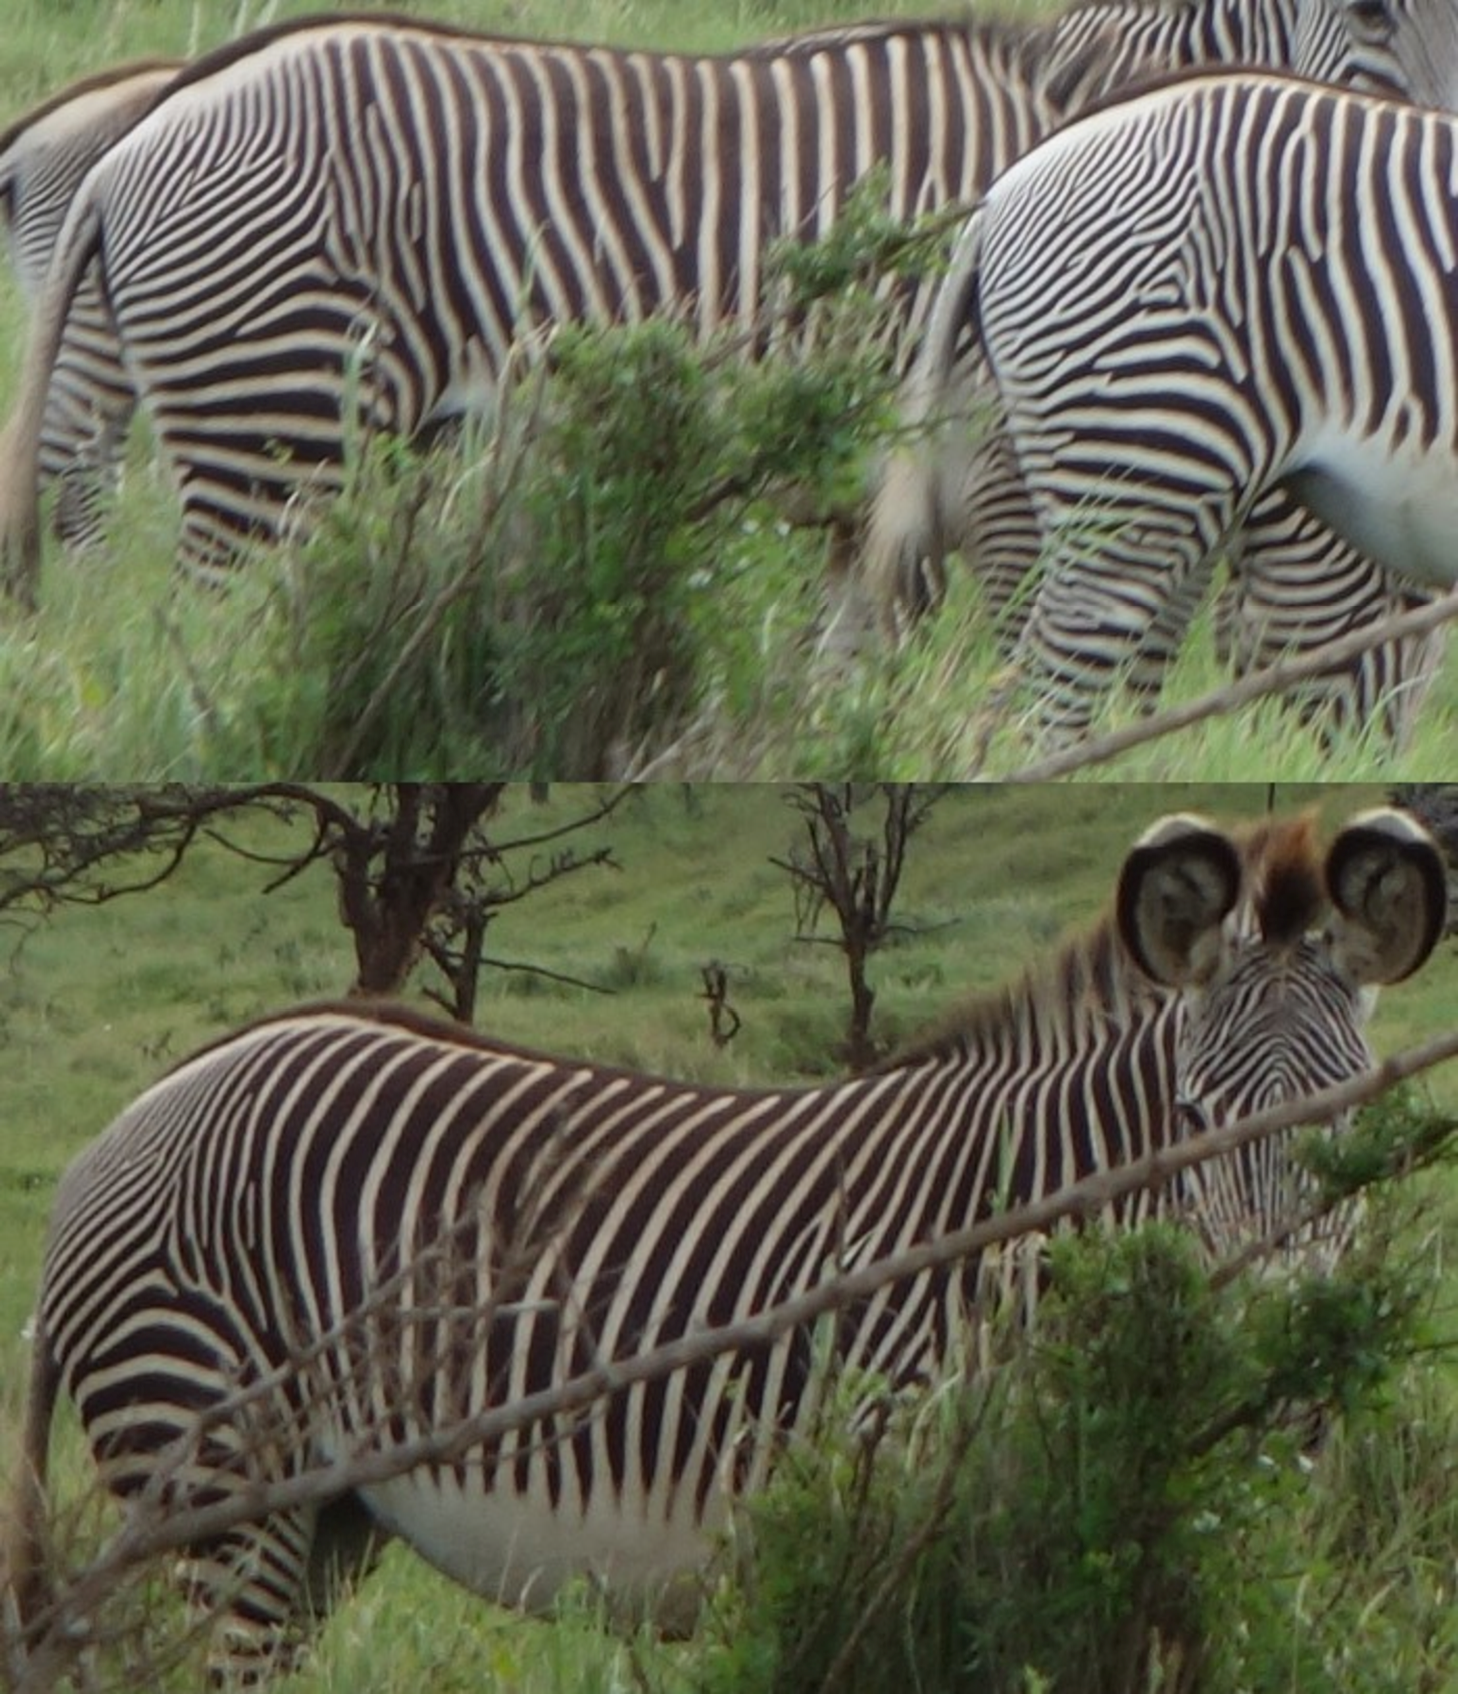
\includegraphics[width=0.20\linewidth]{resources/pair-8451-14771-nca-nca-pos.pdf}  &
            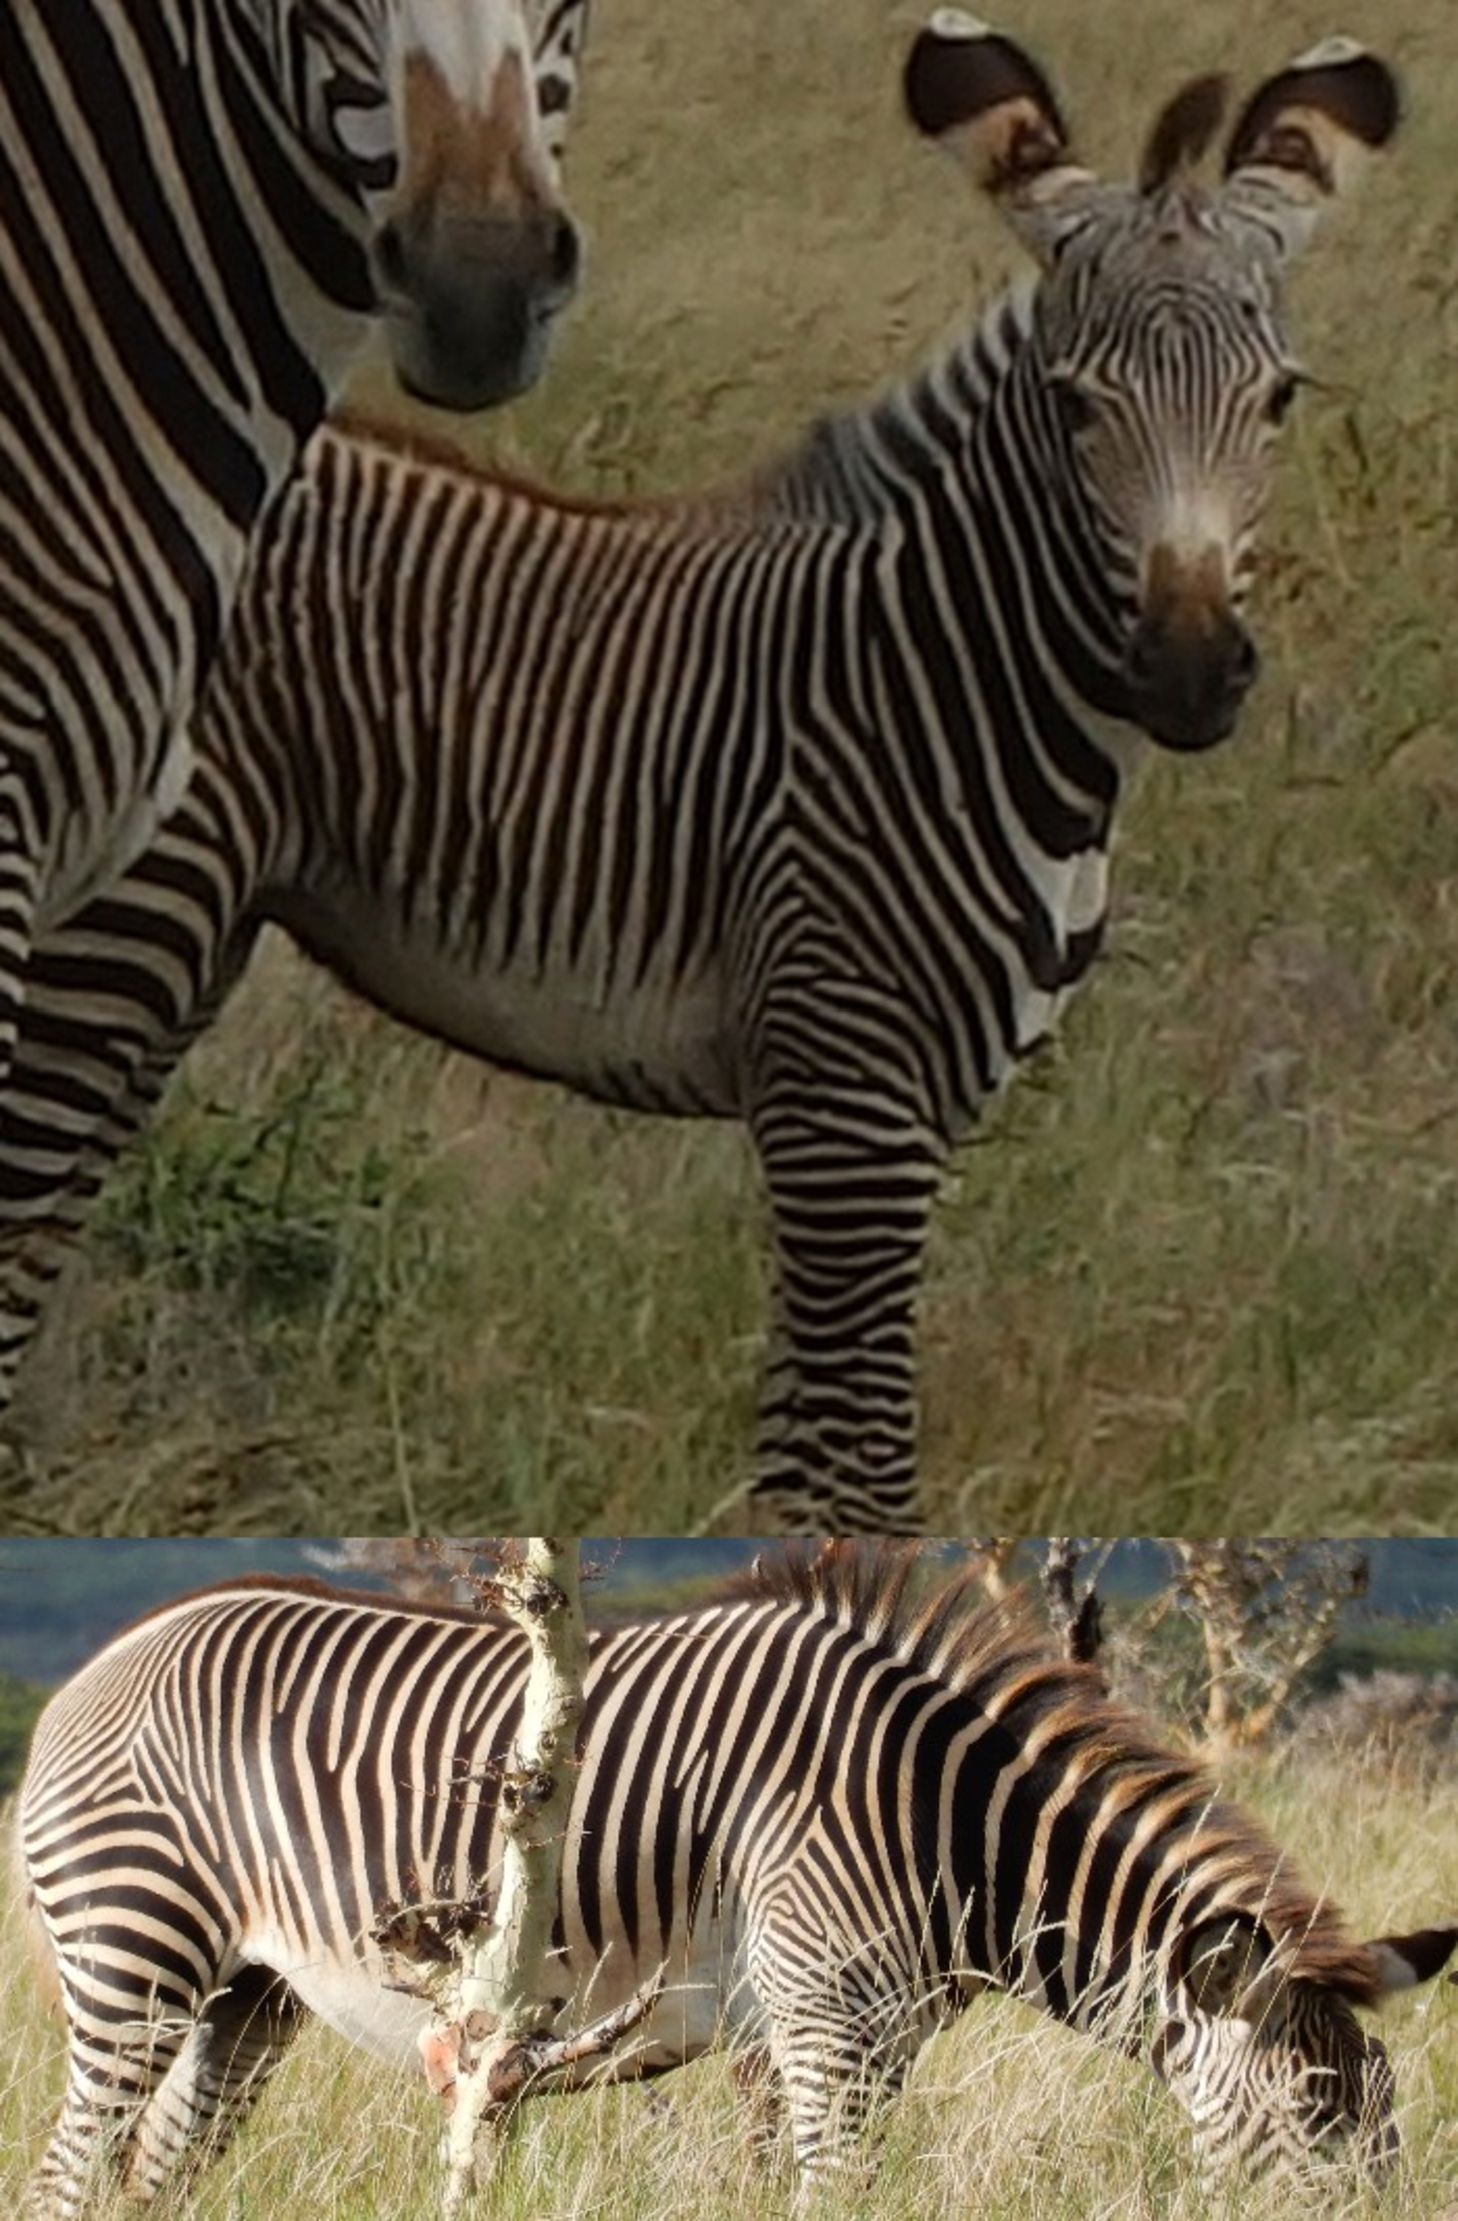
\includegraphics[width=0.20\linewidth]{resources/pair-4071-4887-nca-nca-neg.pdf}   &
            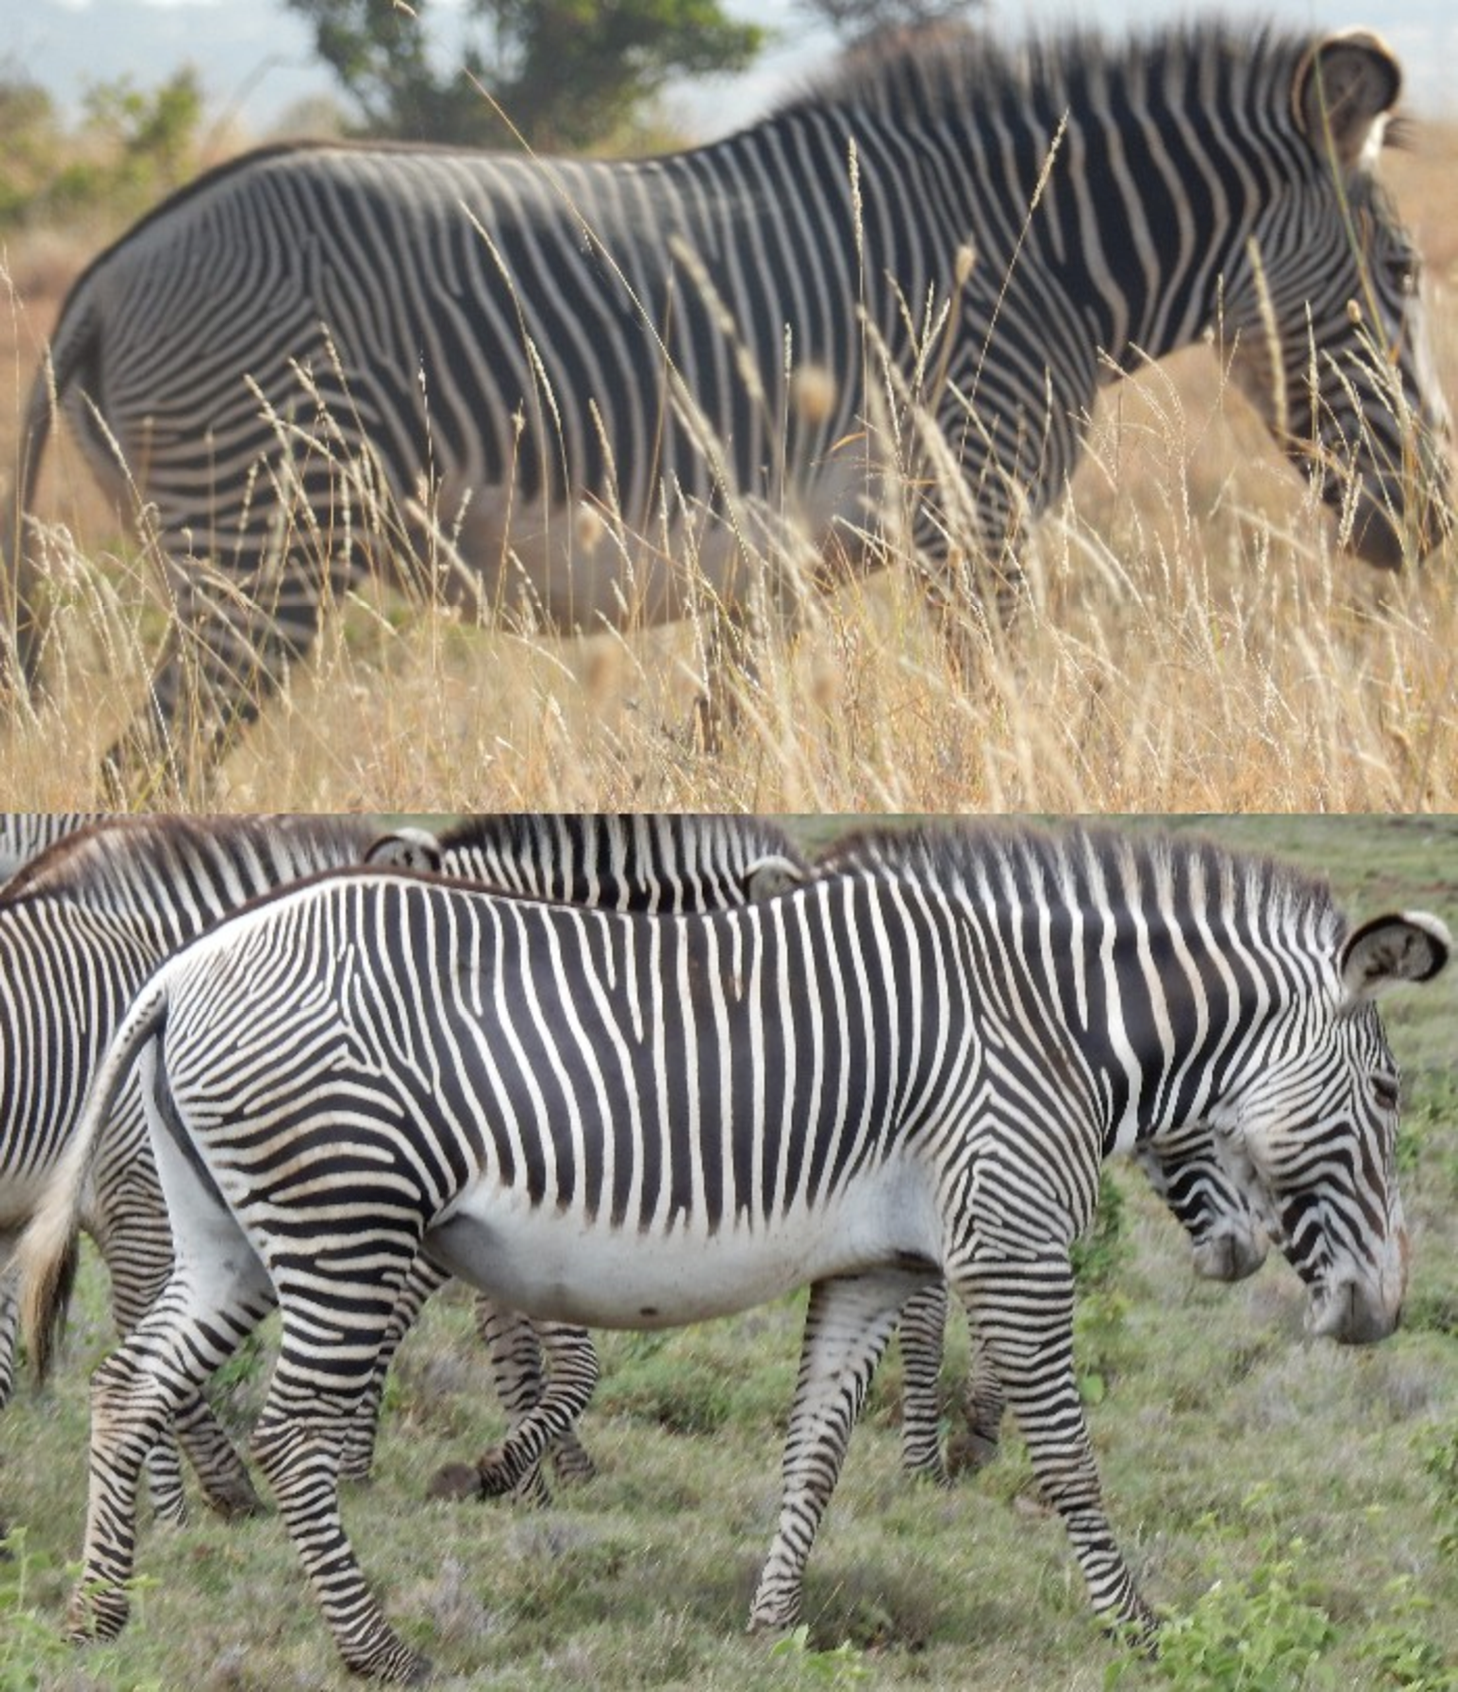
\includegraphics[width=0.20\linewidth]{resources/pair-3074-7992-nca-ca-pos.pdf}    &
            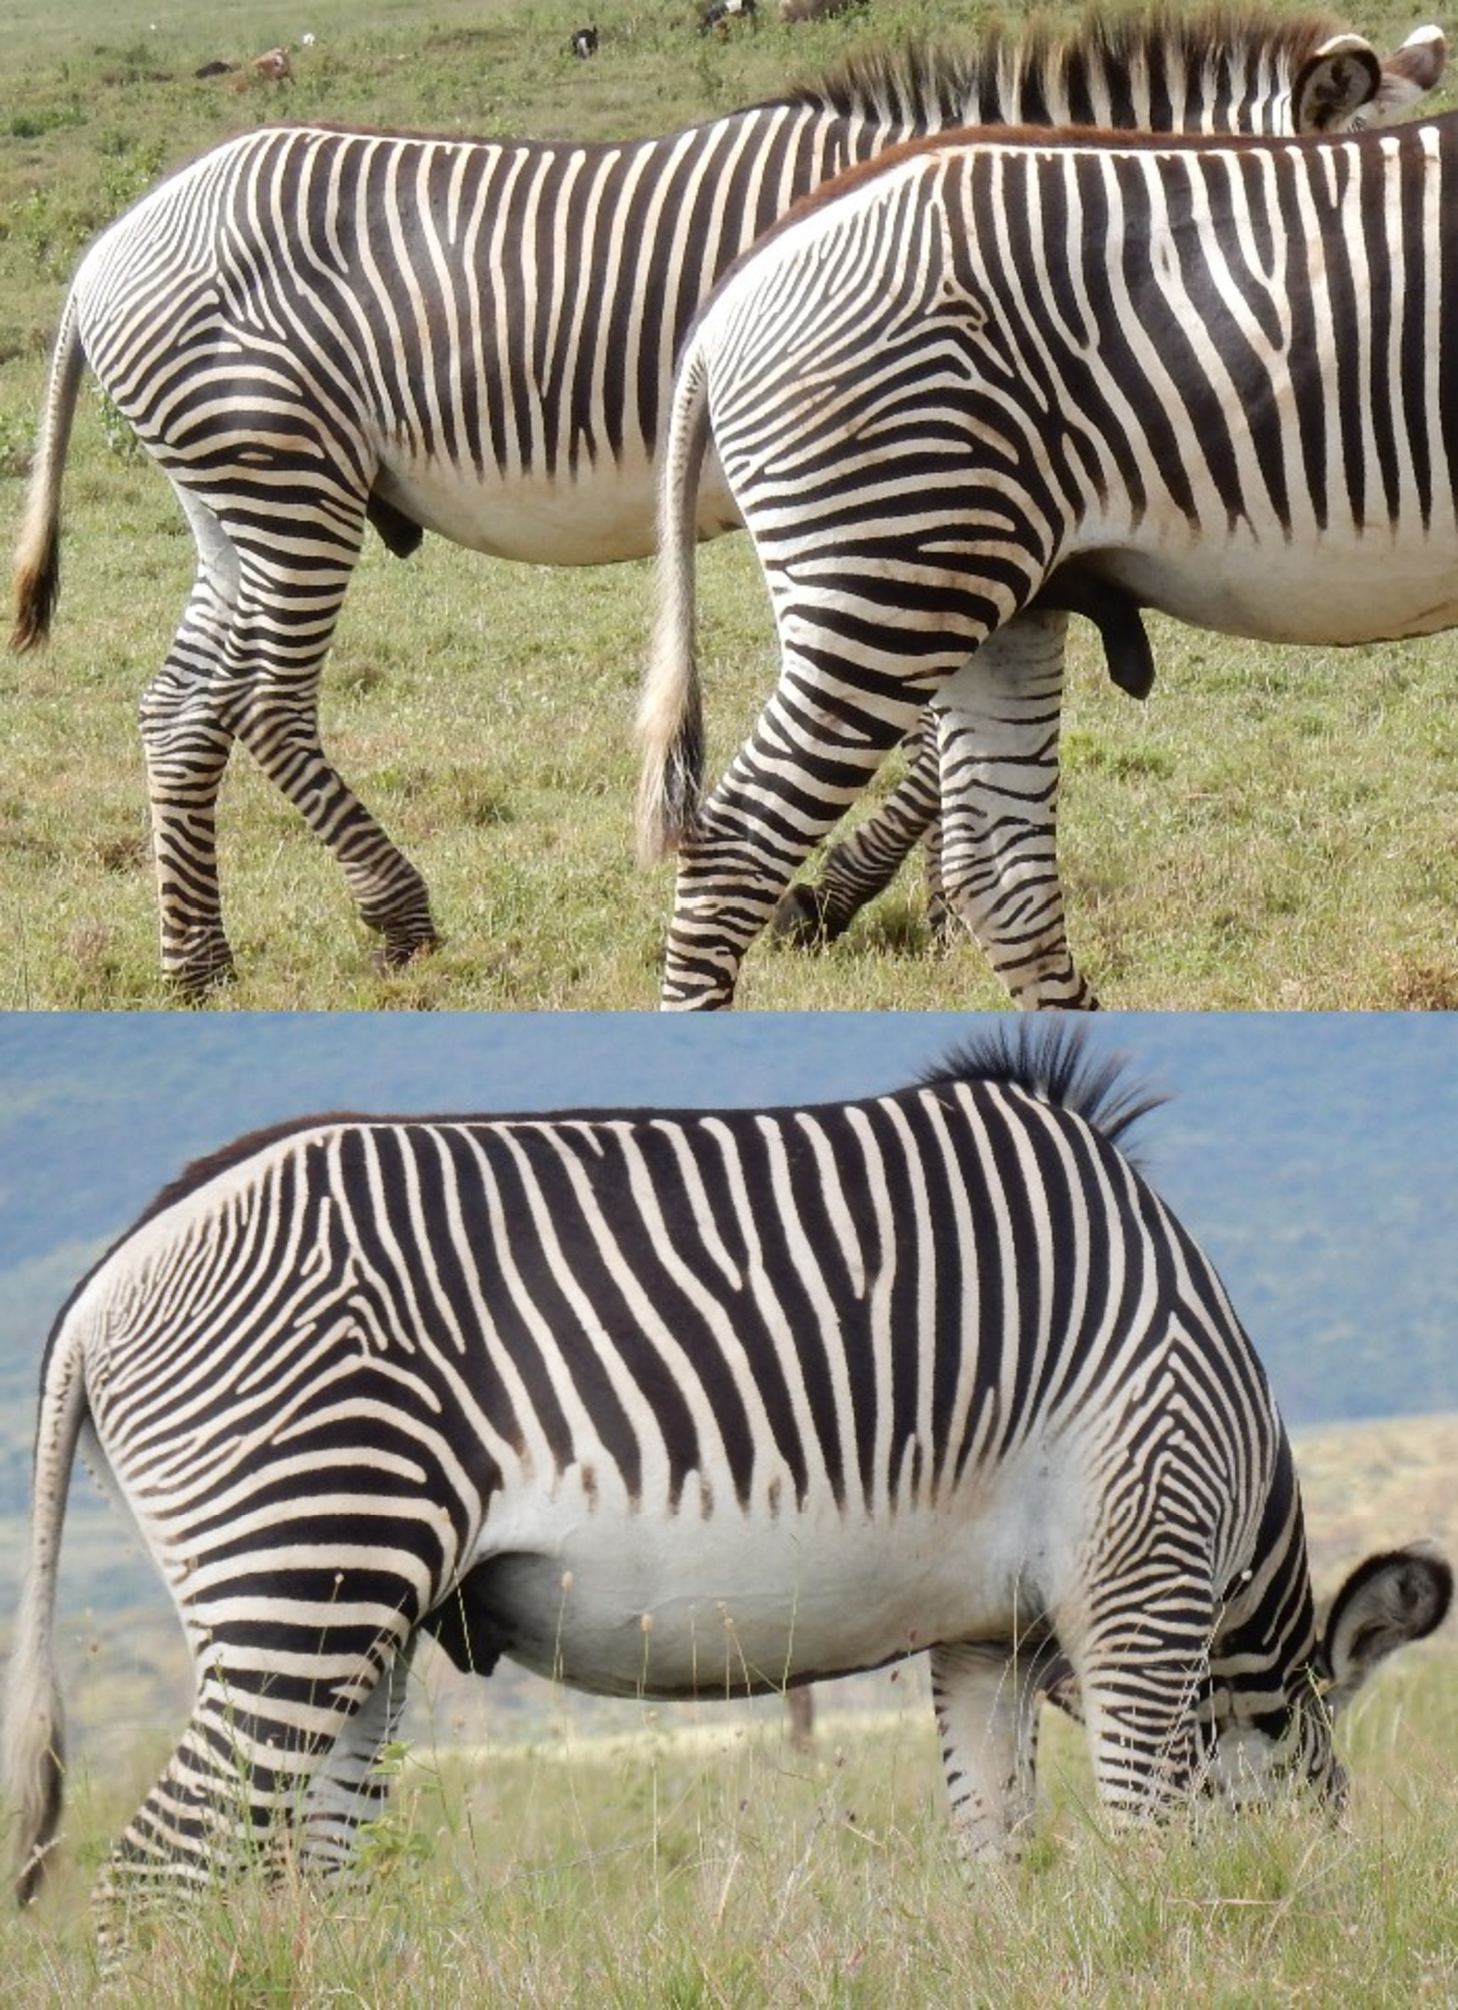
\includegraphics[width=0.20\linewidth]{resources/pair-7979-12732-nca-ca-neg.pdf}     \\
            \textbf{NCA-NCA Positive}                                                          &
            \textbf{NCA-NCA Negative}                                                          &
            \textbf{NCA-CA Positive}                                                           &
            \textbf{NCA-CA Negative}                                                             \\
            \\
            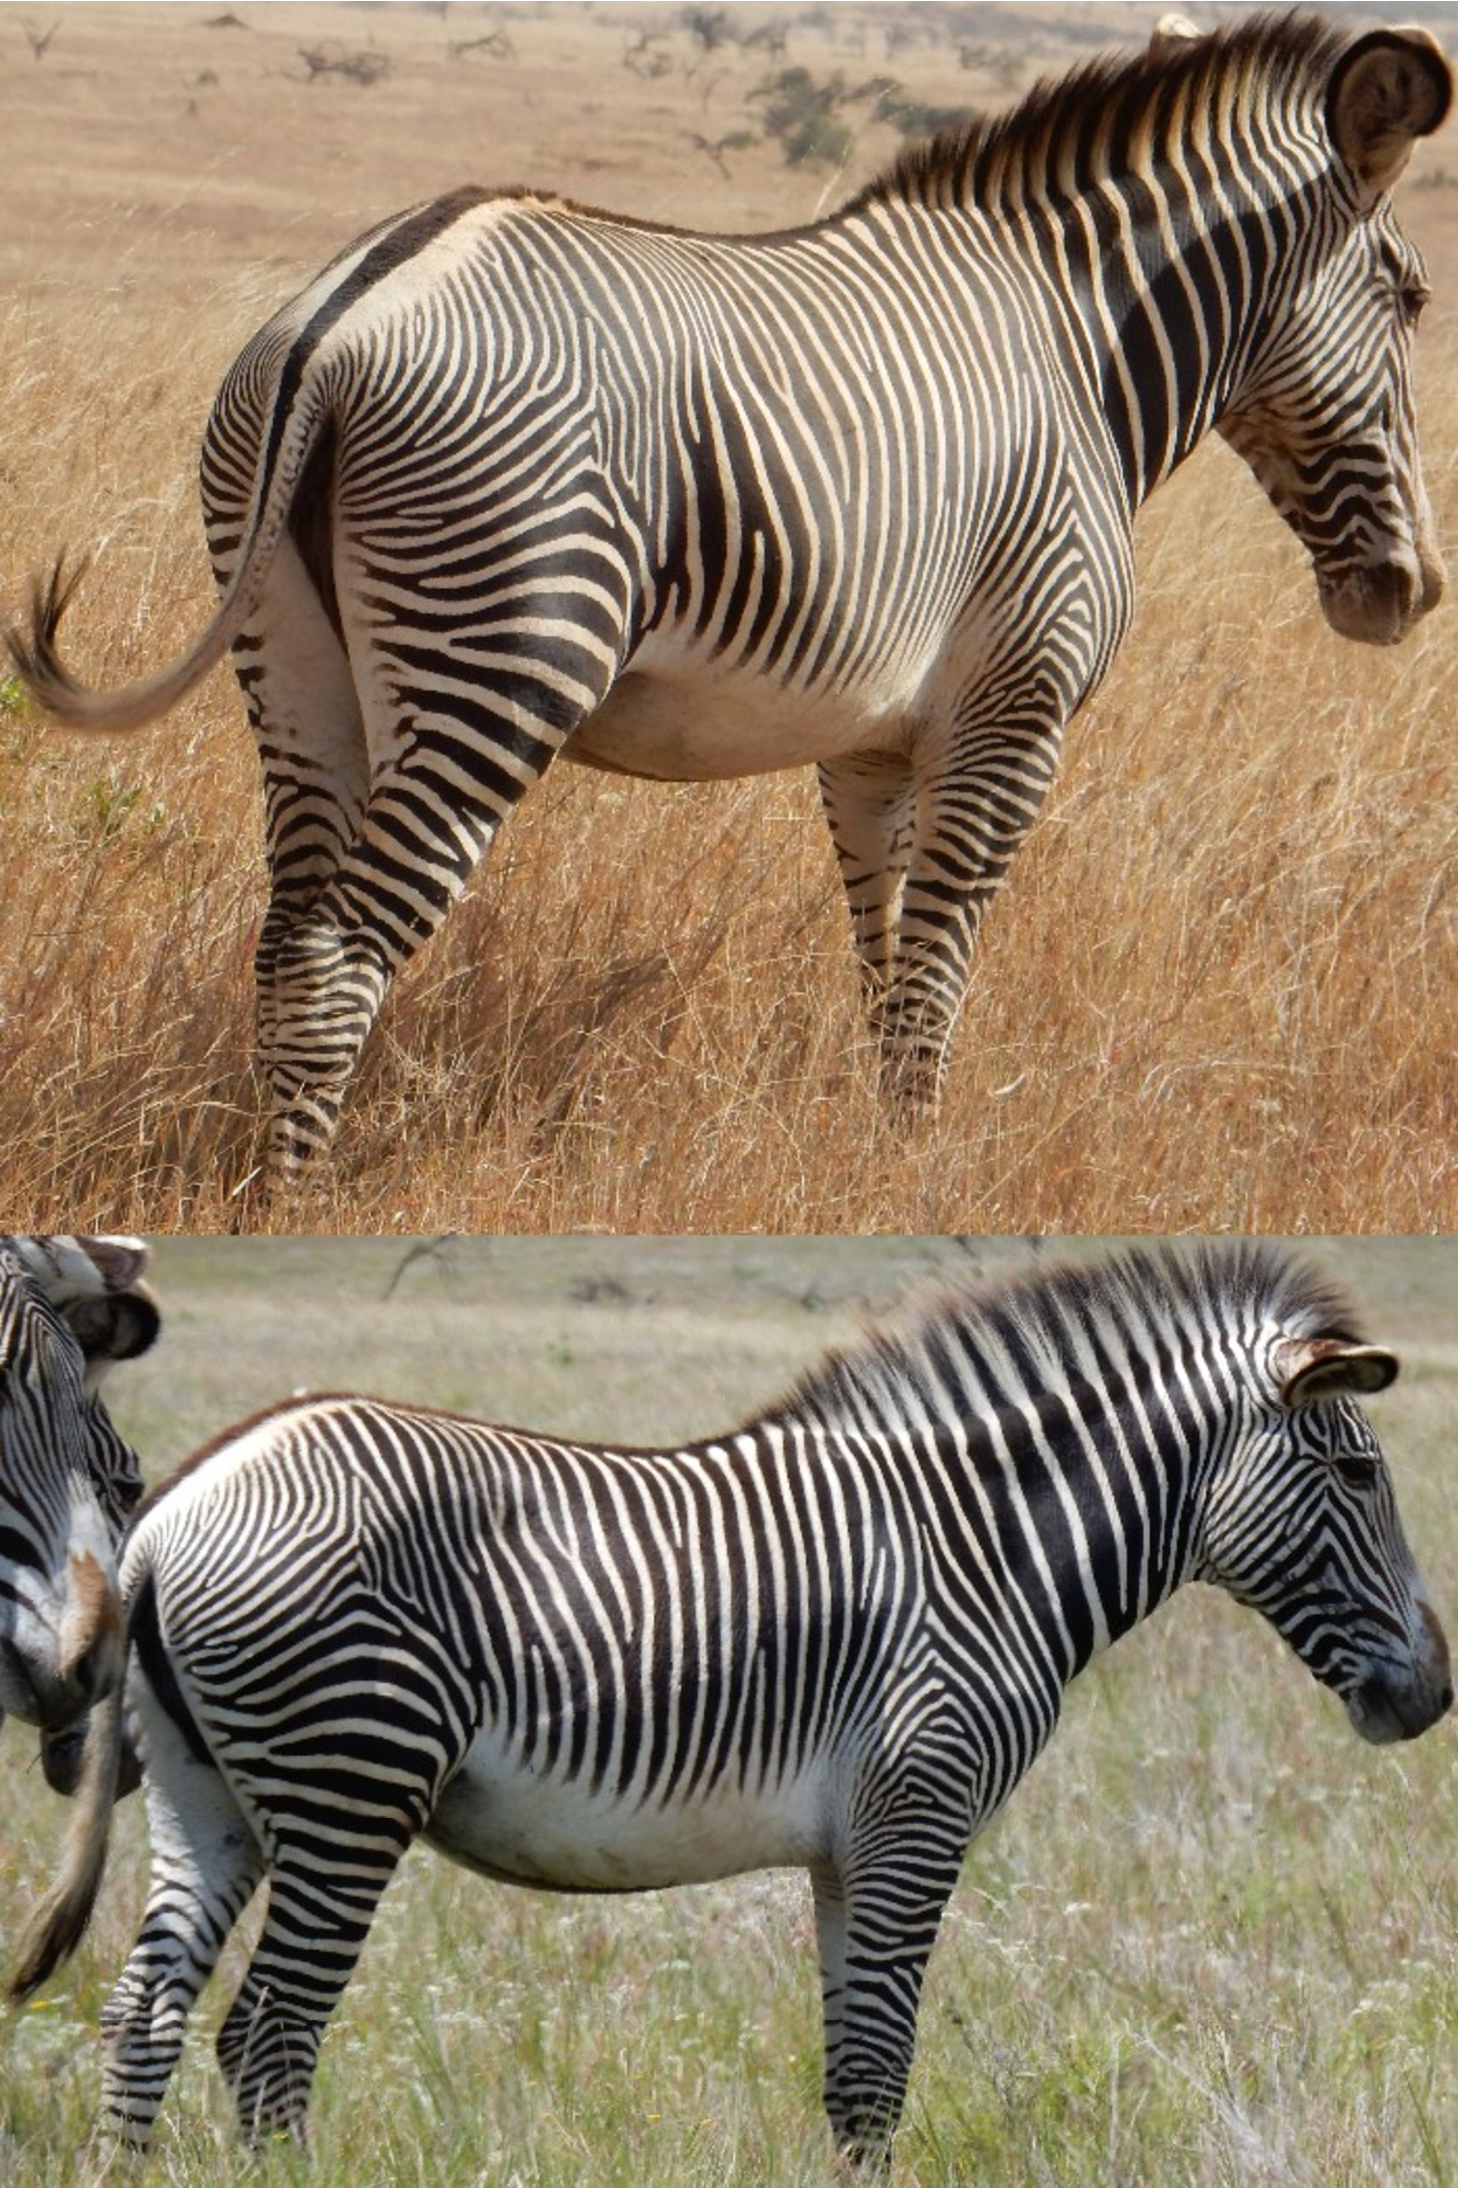
\includegraphics[width=0.20\linewidth]{resources/pair-6083-8515-ca-ca-pos.pdf}     &
            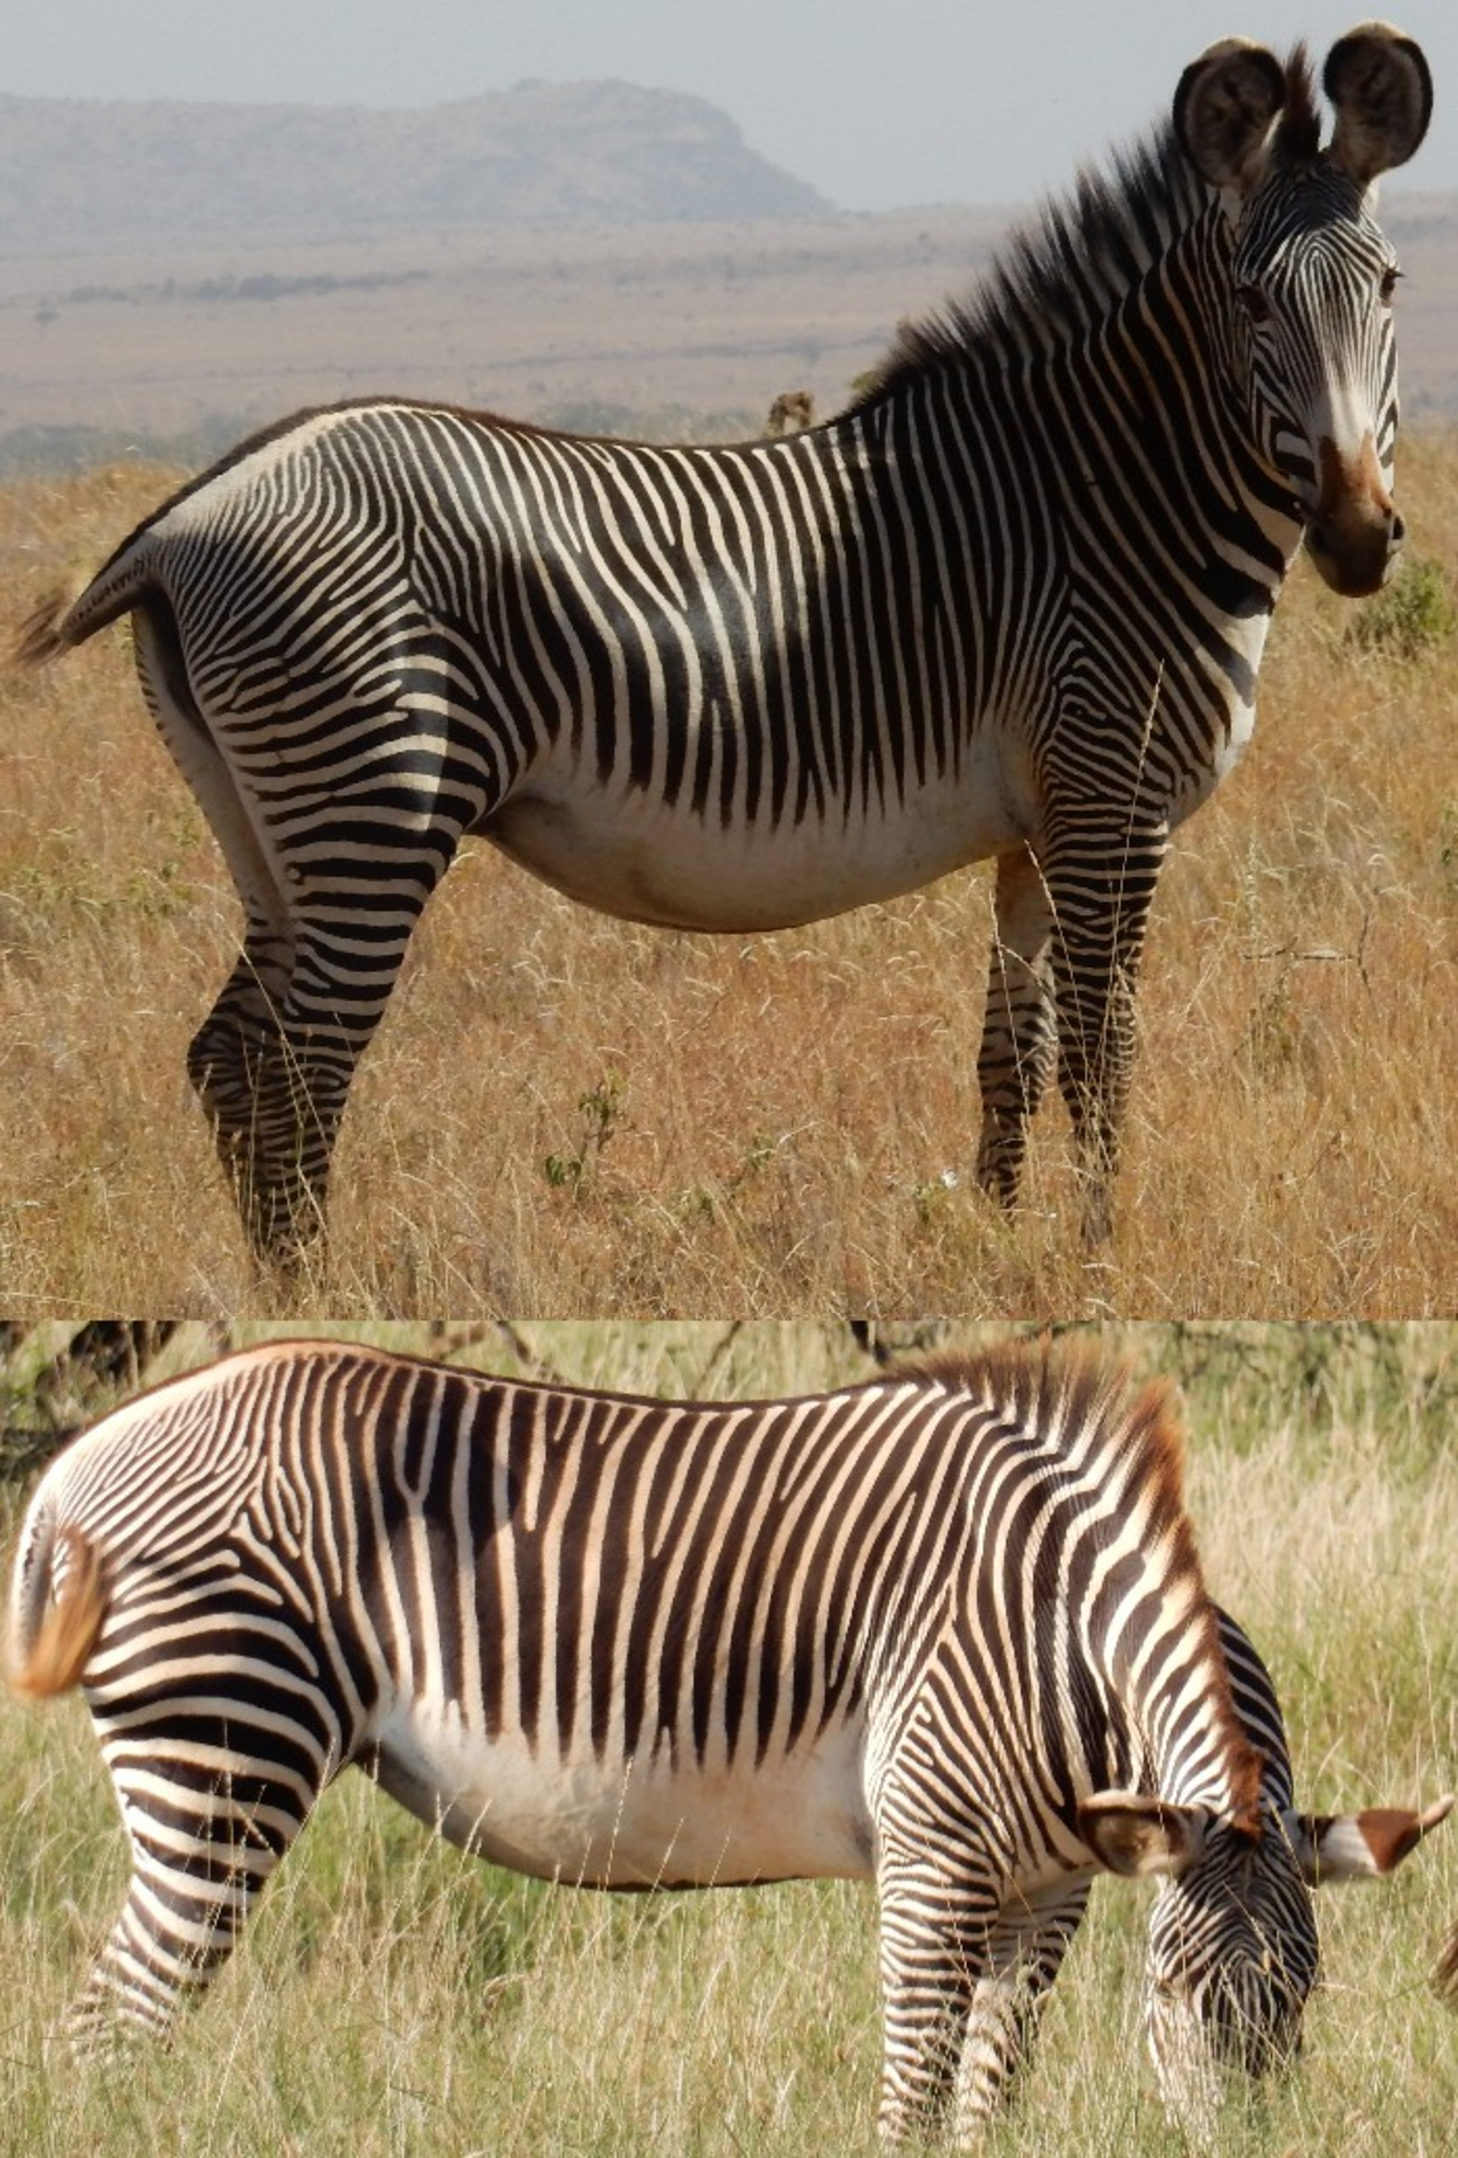
\includegraphics[width=0.20\linewidth]{resources/pair-116-4597-ca-ca-neg.pdf}      &
            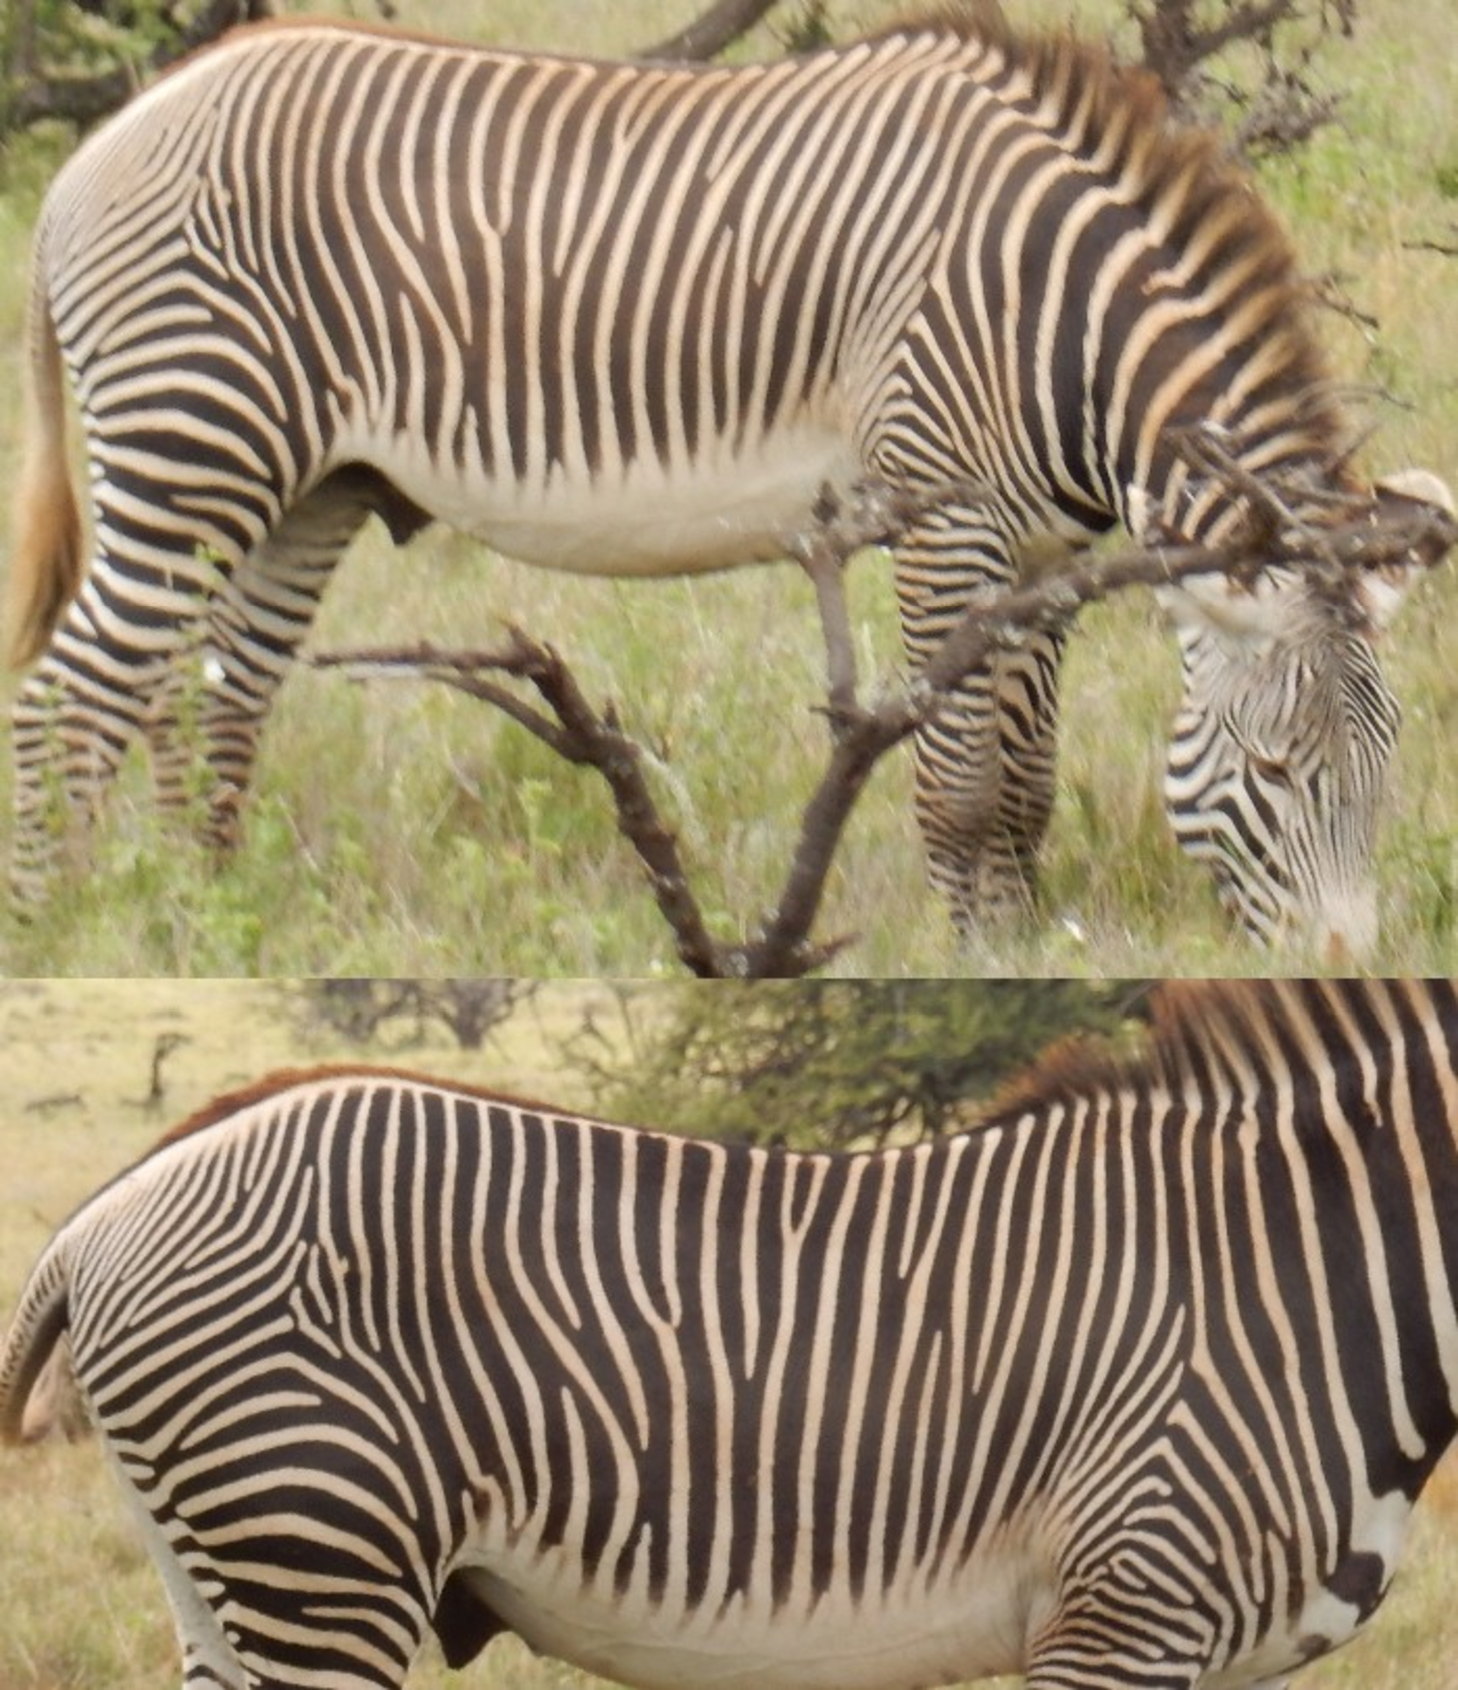
\includegraphics[width=0.20\linewidth]{resources/pair-3615-19342-ca-car-pos.pdf}   &
            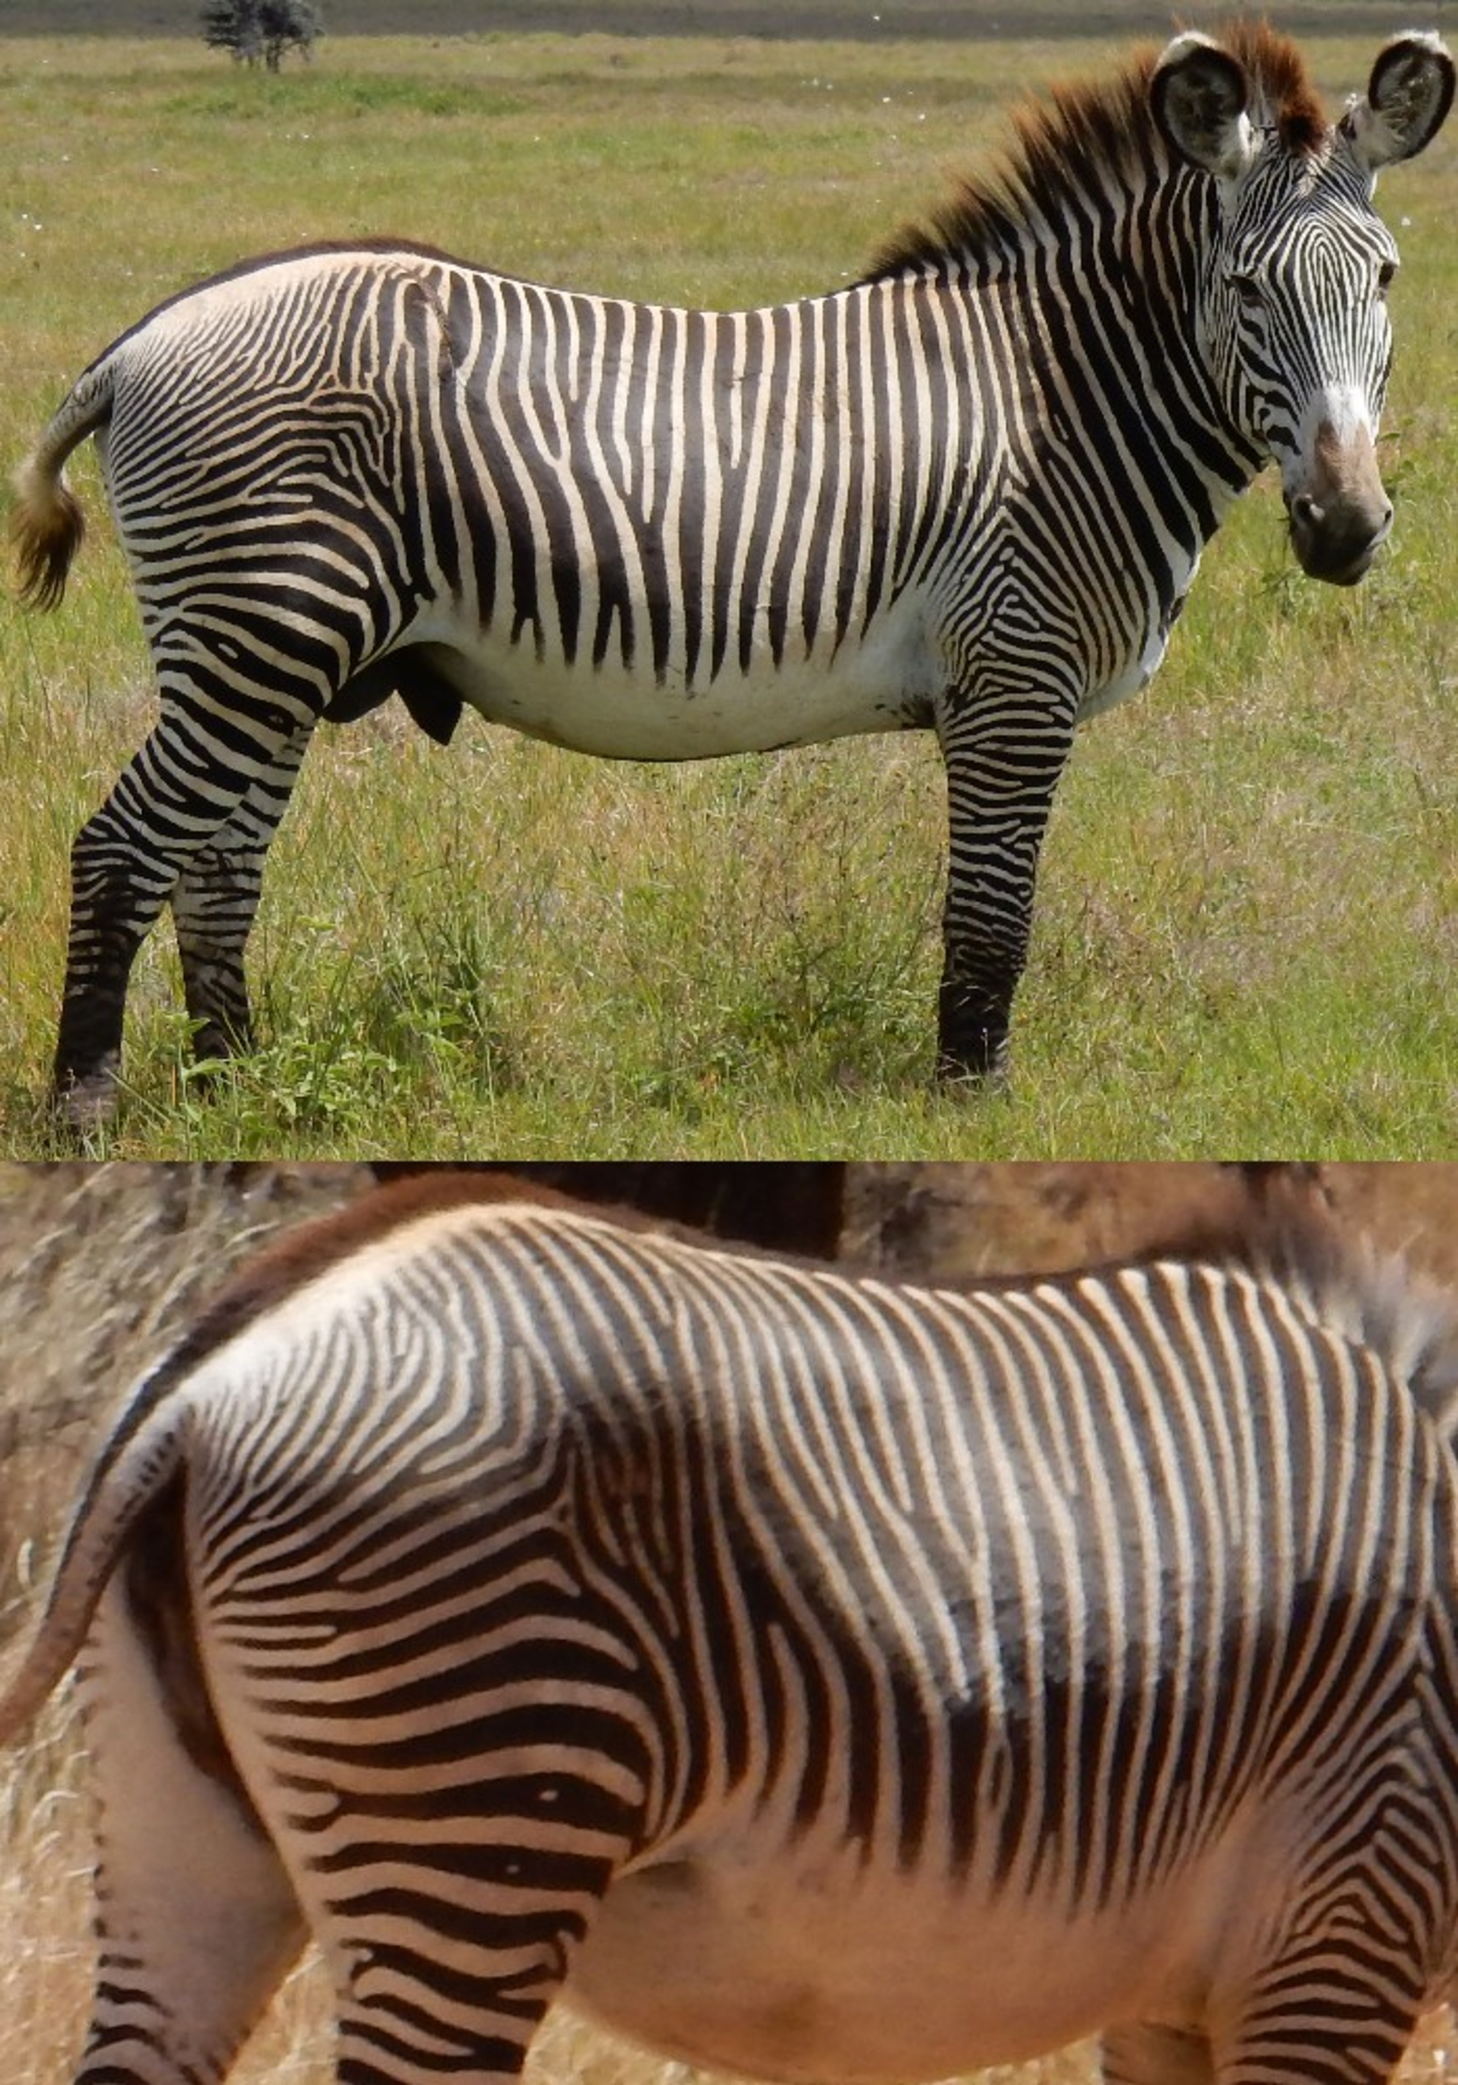
\includegraphics[width=0.20\linewidth]{resources/pair-873-16541-ca-car-neg.pdf}      \\
            \textbf{CA-CA Positive}                                                            &
            \textbf{CA-CA Negative}                                                            &
            \textbf{CA-CAR Positive}                                                           &
            \textbf{CA-CAR Negative}                                                             \\
            \\
            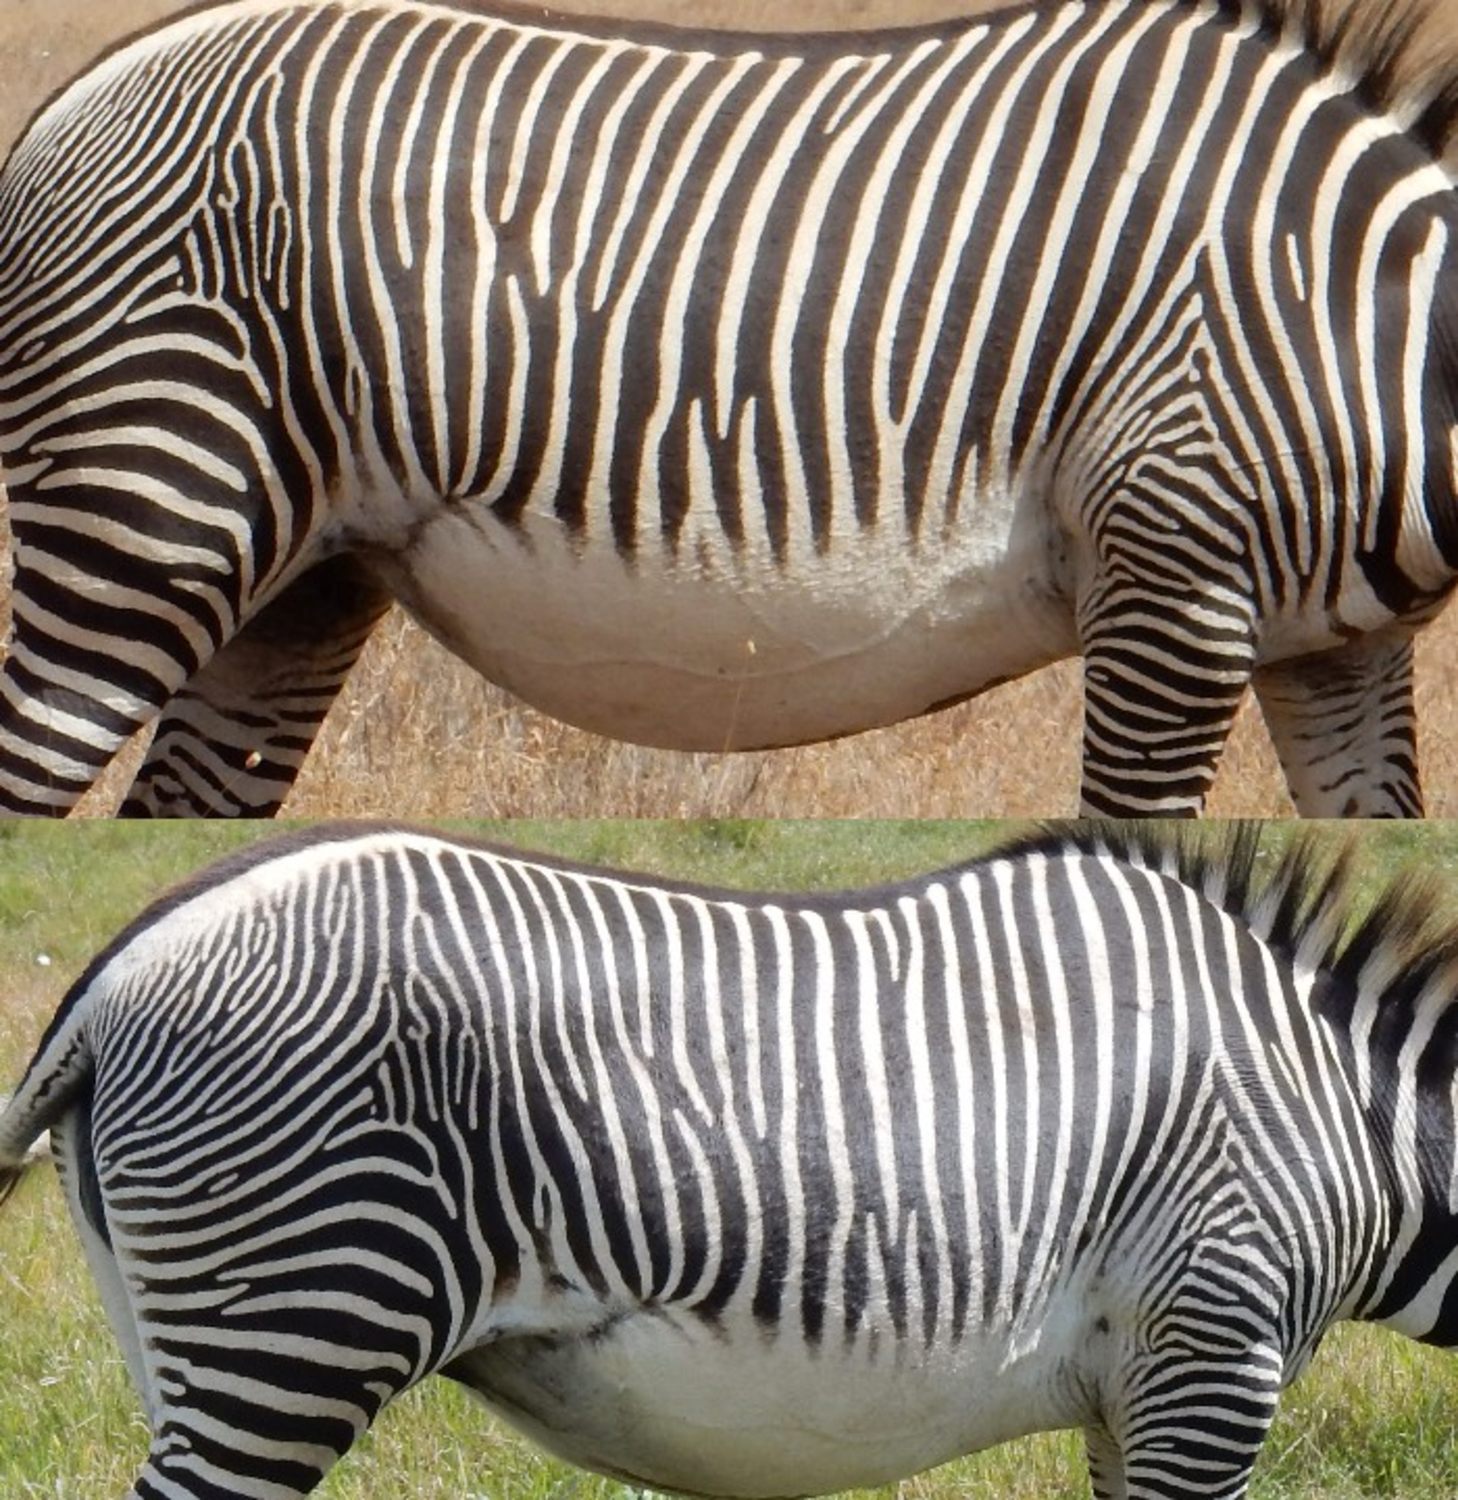
\includegraphics[width=0.20\linewidth]{resources/pair-16277-17725-car-car-pos.pdf} &
            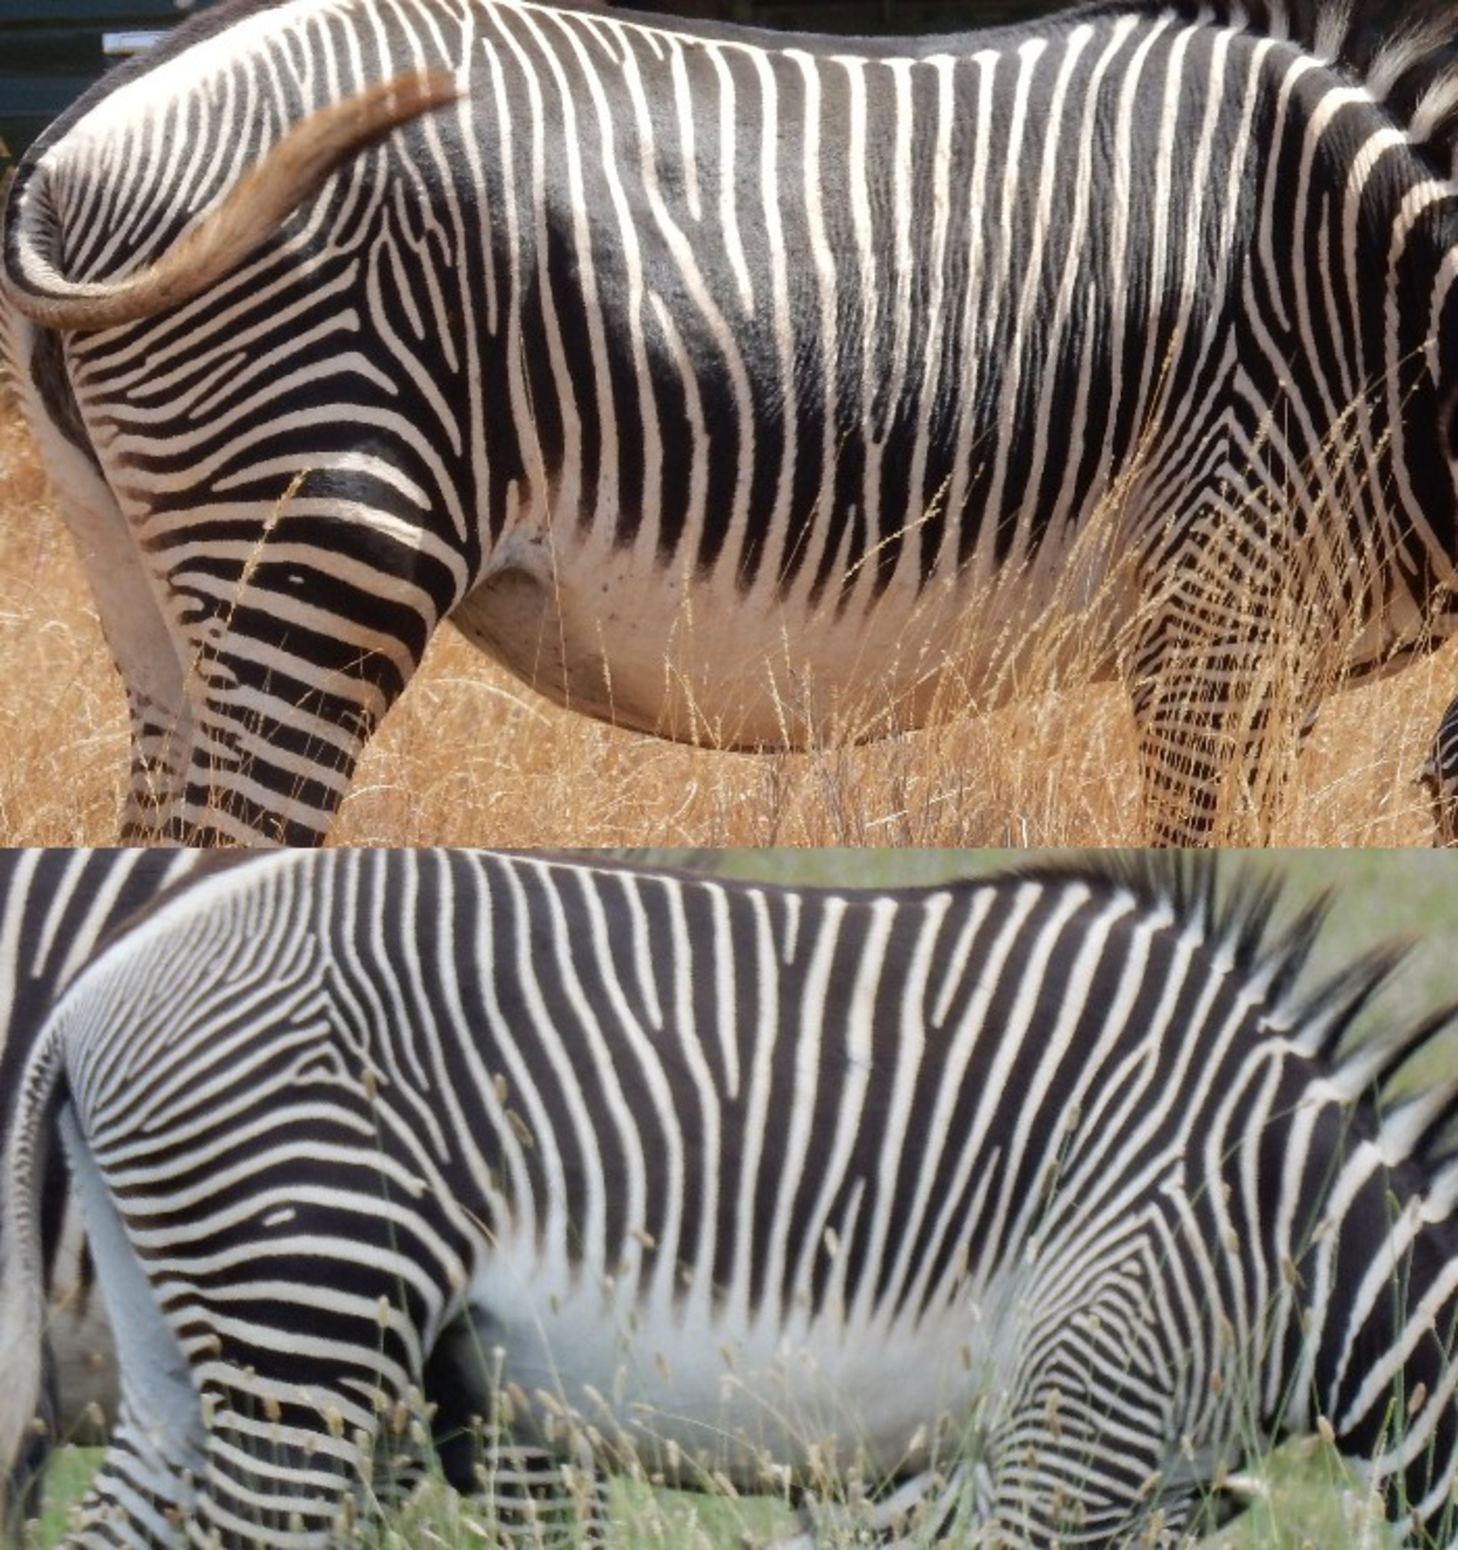
\includegraphics[width=0.20\linewidth]{resources/pair-15704-17583-car-car-neg.pdf} &
            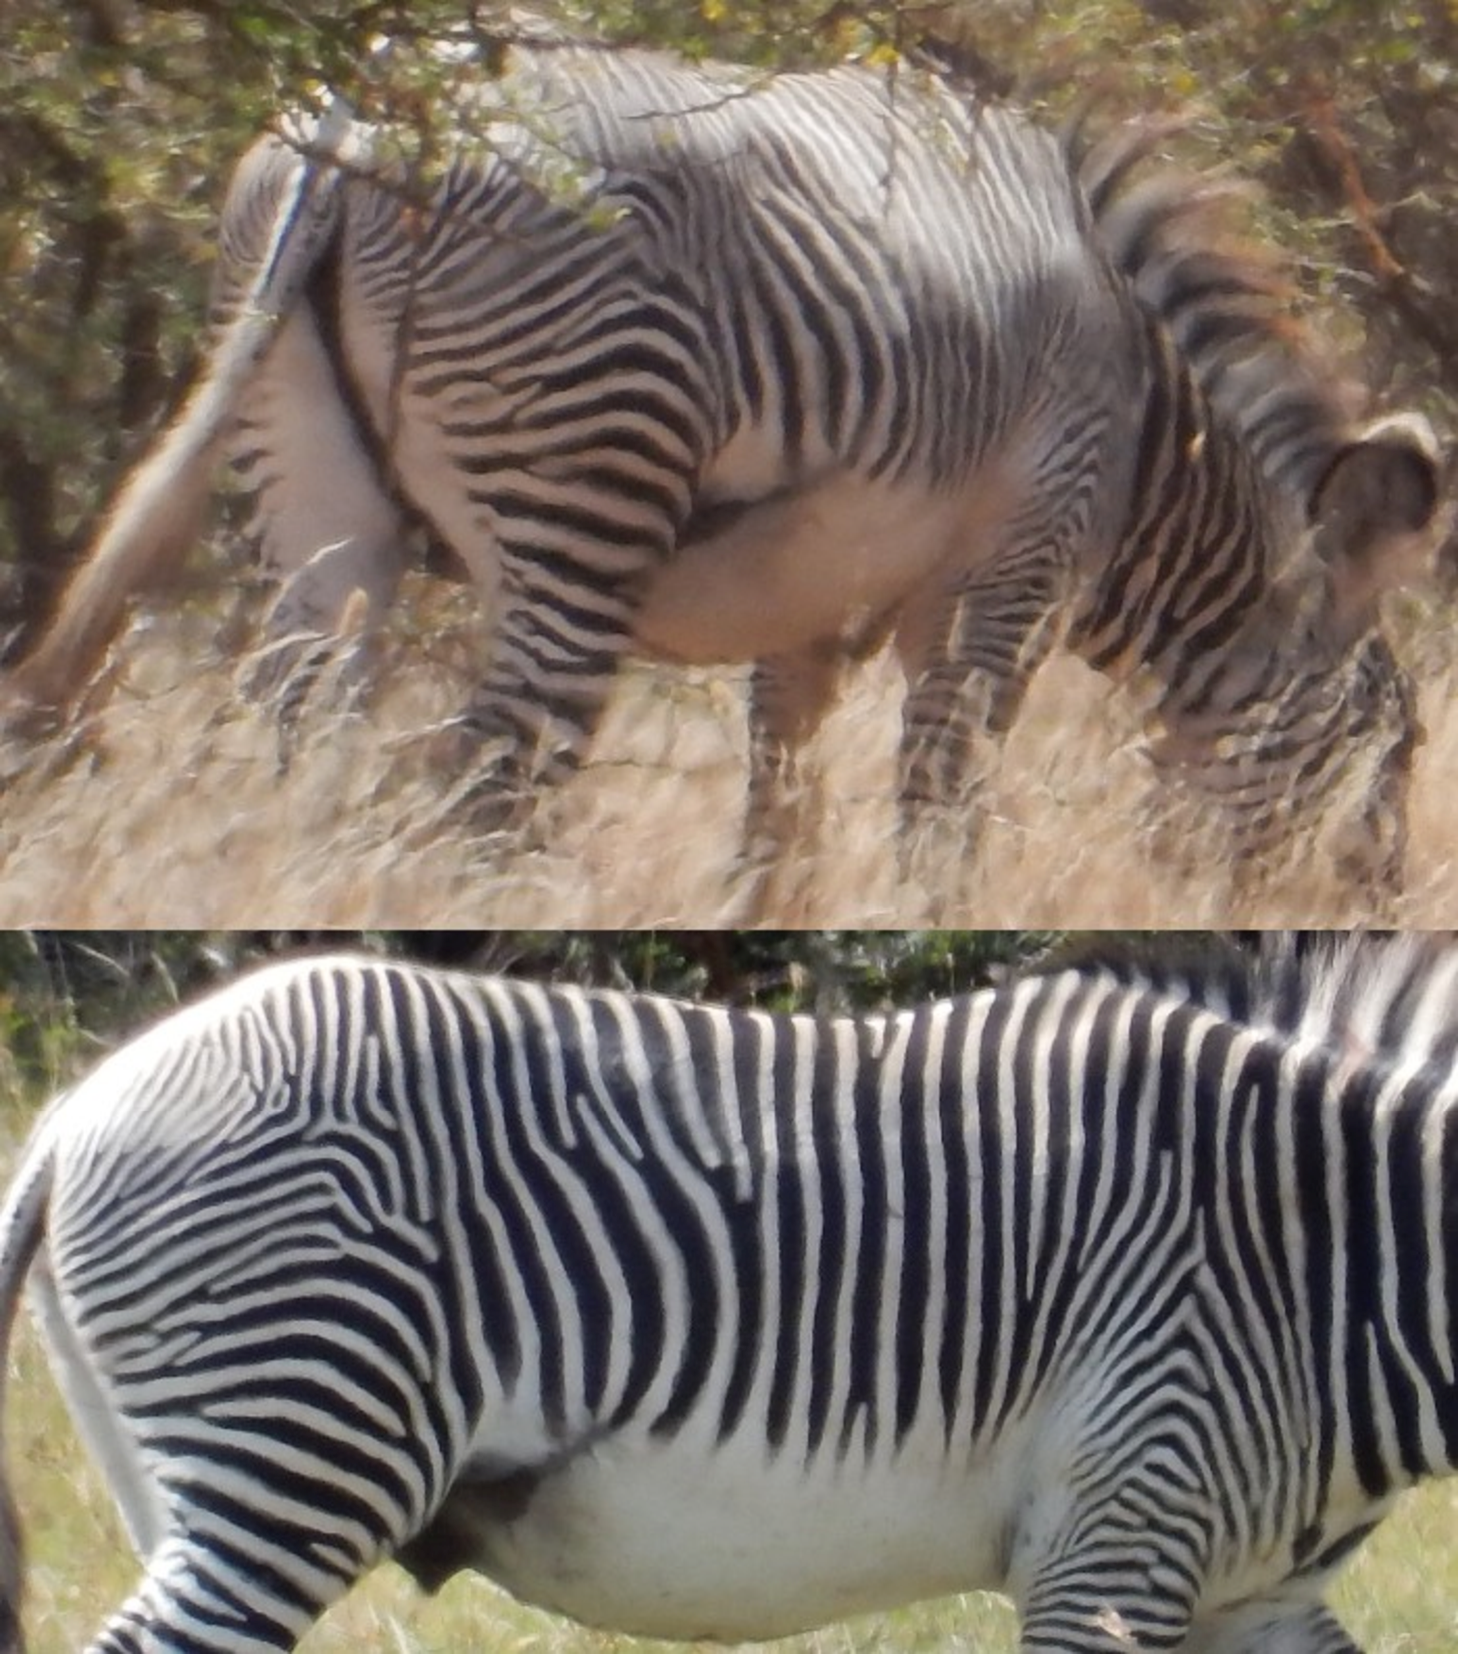
\includegraphics[width=0.20\linewidth]{resources/pair-2347-19088-nca-car-pos.pdf}  &
            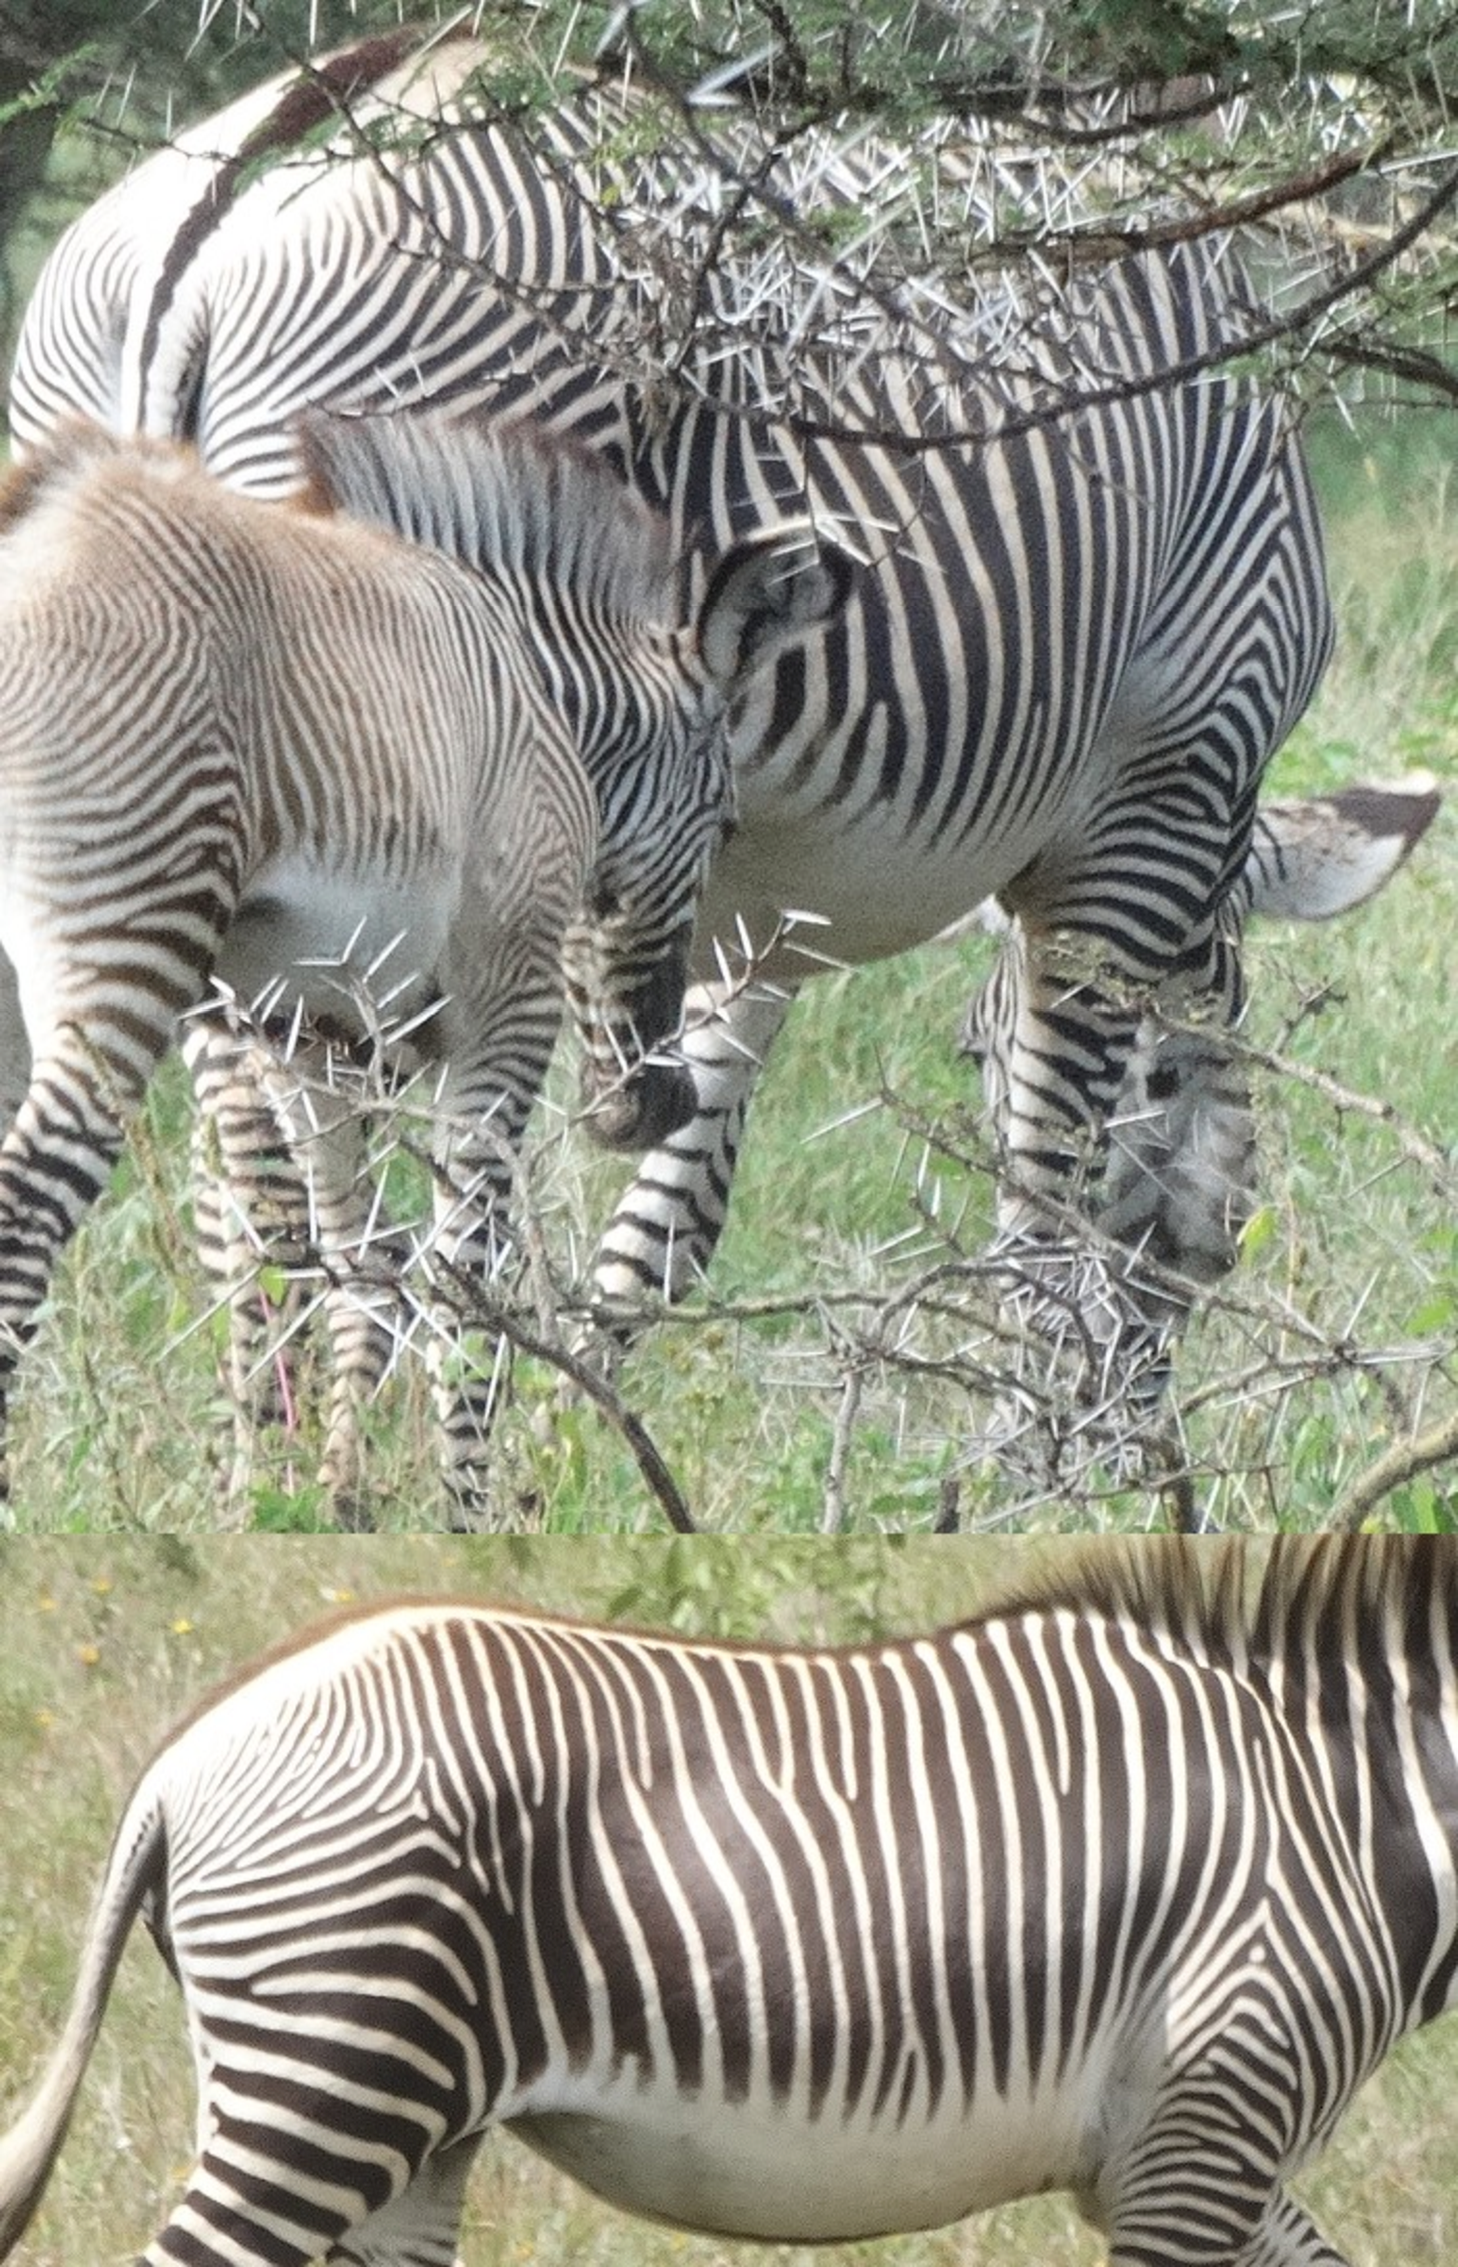
\includegraphics[width=0.20\linewidth]{resources/pair-9132-17155-nca-car-neg.pdf}    \\
            \textbf{CAR-CAR Positive}                                                          &
            \textbf{CAR-CAR Negative}                                                          &
            \textbf{NCA-CAR Positive}                                                          &
            \textbf{NCA-CAR Negative}
        \end{tabular}
    \end{center}
    \caption{Example match pairs used during the user study.  The user study was designed to test the impact of Census Annotation and Census Annotation Regions on human verification, measuring the accuracy and time it took to review 300 total pairs.  The expectation is that a reviewer will have the most difficulty (and therefore spend the most time) with NCA-NCA pairs and perform the best with CAR-CAR pairs.}
    \label{fig:nca-ca-car-pairs}
\end{figure}

We need to determine if using Census Annotations in a photographic census positively impacts a human's ability to decide the matched pairs sent to review.  Specifically, we need to know if CAs or CA Regions 1) improve the accuracy of manual verification and 2) reduce the total amount of time it takes to make a decision.  With an automated population census, the primary goal is to minimize the number of verification decisions needed from humans.  When human work is needed, though, there is a secondary goal of minimizing the complexity of the verification task; this is important because we can expect that an easier decision will end up being faster, thus reducing the total on-task time for humans.  The GZCD provides a ground-truth dataset of hundreds of animal IDs, with some of them containing relatively poor-quality annotations.  The dataset is mined for pairs that range from being easy to review (a pair between two Census Annotation Regions) to hard to review (a matched pair between two non-CAs) to evaluate the performance of humans on reviewing pairs.  For simplicity, this section will refer to any annotation that is not a CA as a ``non-CA''  or ``NCA''.  Furthermore, a Census Annotation will be referred to as a ``CA'', like usual, and a CA Regions as a ``CAR'' (without the ordinary hyphen).  Match pairs between two annotations will be (conveniently) denoted with a hyphen.  For example, a ``CA-CAR'' pair contains one Census Annotation and one Census Annotation Region, and the ordering does not matter.  Having three possible states for an annotation produces a combination of 6 possible pair types to collect for this user study:

\squishlist
\item \textbf{NCA-NCA} - a non-CA and non-CA pair
\item \textbf{NCA-CA} - a non-CA and CA pair
\item \textbf{NCA-CAR} - a non-CA and CA Region pair
\item \textbf{CA-CA} - a CA and CA pair
\item \textbf{CA-CAR} - a CA and CA Region pair
\item \textbf{CAR-CAR} - a CA Region and CA Region pair
\squishend

For each of the six types of pairs, there are ground-truth ``same animal'' (positive) examples or ``different animals'' (negative) examples, resulting in 12 total options for the study.  To properly sample the various combinations of pair types, all of the named annotations (10,037 total, 4,762 named CA Regions) in the GZCD (that also had an acceptable quality) were selected.  This filtering resulted in a set of 9,966 annotations and CA Regions to mine for match pairs: 1,692 NCAs, 4,142 CAs (as determined by a threshold of 0.31), and 4,142 corresponding CA-Rs.  All of the ${9966 \choose 2}$ pair combinations (49.6 million in total) were enumerated and were randomly shuffled.  The random collection was then traversed, and pairs were gathered for each of the 12 categories.  The pair's category was determined by 1) the ground-truth NCA, CA, or CA-R status of its annotations and 2) a ``same animal'' or ``different animal'' decision from the ground-truth name IDs between its annotations.  The process continued until 25 examples for each category were found, generating a total of 300 pairs.  An additional constraint on the mining process required all 600 annotations (two per pair) to be unique.  Figure~\ref{fig:nca-ca-car-pairs} shows an example for each of the 12 types.  A final check was performed by hand to ensure that none of the 300 pairs were accidentally incomparable. Each pair was guaranteed to be decidable given enough time and subject to the expertise of the individual user in the study.

The collection of 300 test pairs was then given to six independent reviewers.  Three reviewers in the study are considered ``experts'' in reviewing pairs of Gr\'evy's zebra matches, each with the real-world experience of reviewing thousands of match decisions.  Three additional ``novice'' reviewers were also added to the study -- two with zero experience with the problem domain and task -- and functioned as a way to control for task experience.  A web-based interface was created that allows each user to annotate a ``same animal'' or ``different animal'' decision for each pair, one at a time.  The web application measured the total turn-around decision time and recorded the accuracy of each decision.  The time between decisions was not tracked (i.e., a reviewer had to request the next match manually) and was allowed to take breaks as needed.  The decisions were made blind without indicating the correct decision and without any algorithmic hints or highlighting where the two annotations may have matched.  The users were provided with a brief training session of approximately ten pairs to understand the task and interface and were told that exactly 50\% of the matches were ``same animal,'' and 50\% were ``different animals''.  The ordering of the match pairs was randomized between each user, and the user was instructed to make decisions at the fastest pace possible while also making as few errors as possible.

Between the six participants in the study, some reviewers were very fast (6.1 seconds per decision) while others were slower (15.9 seconds).  The web interface was optimized with pre-rendered images. Each user's decisions were collected at non-overlapping times, and the webserver used the same hardware setup for all participants.  What was not controlled for was the total round-trip travel time of the loaded web content over the Internet or the various computers, browsers, and medium that each participant used.  For example, one participant was located in the same city as the webserver, while another was located three time zones away and in a different country at the time of their participation.  However, a constant delay experienced by a given user during the study is expected to be somewhat reliable.  All users completed their participation in the study in less than 90 total active minutes and freely volunteered their time without financial compensation.  For transparency, the author of this dissertation and his Ph.D.\ advisor both participated as ``expert'' users.

\begin{figure}[!t]
    \begin{center}
        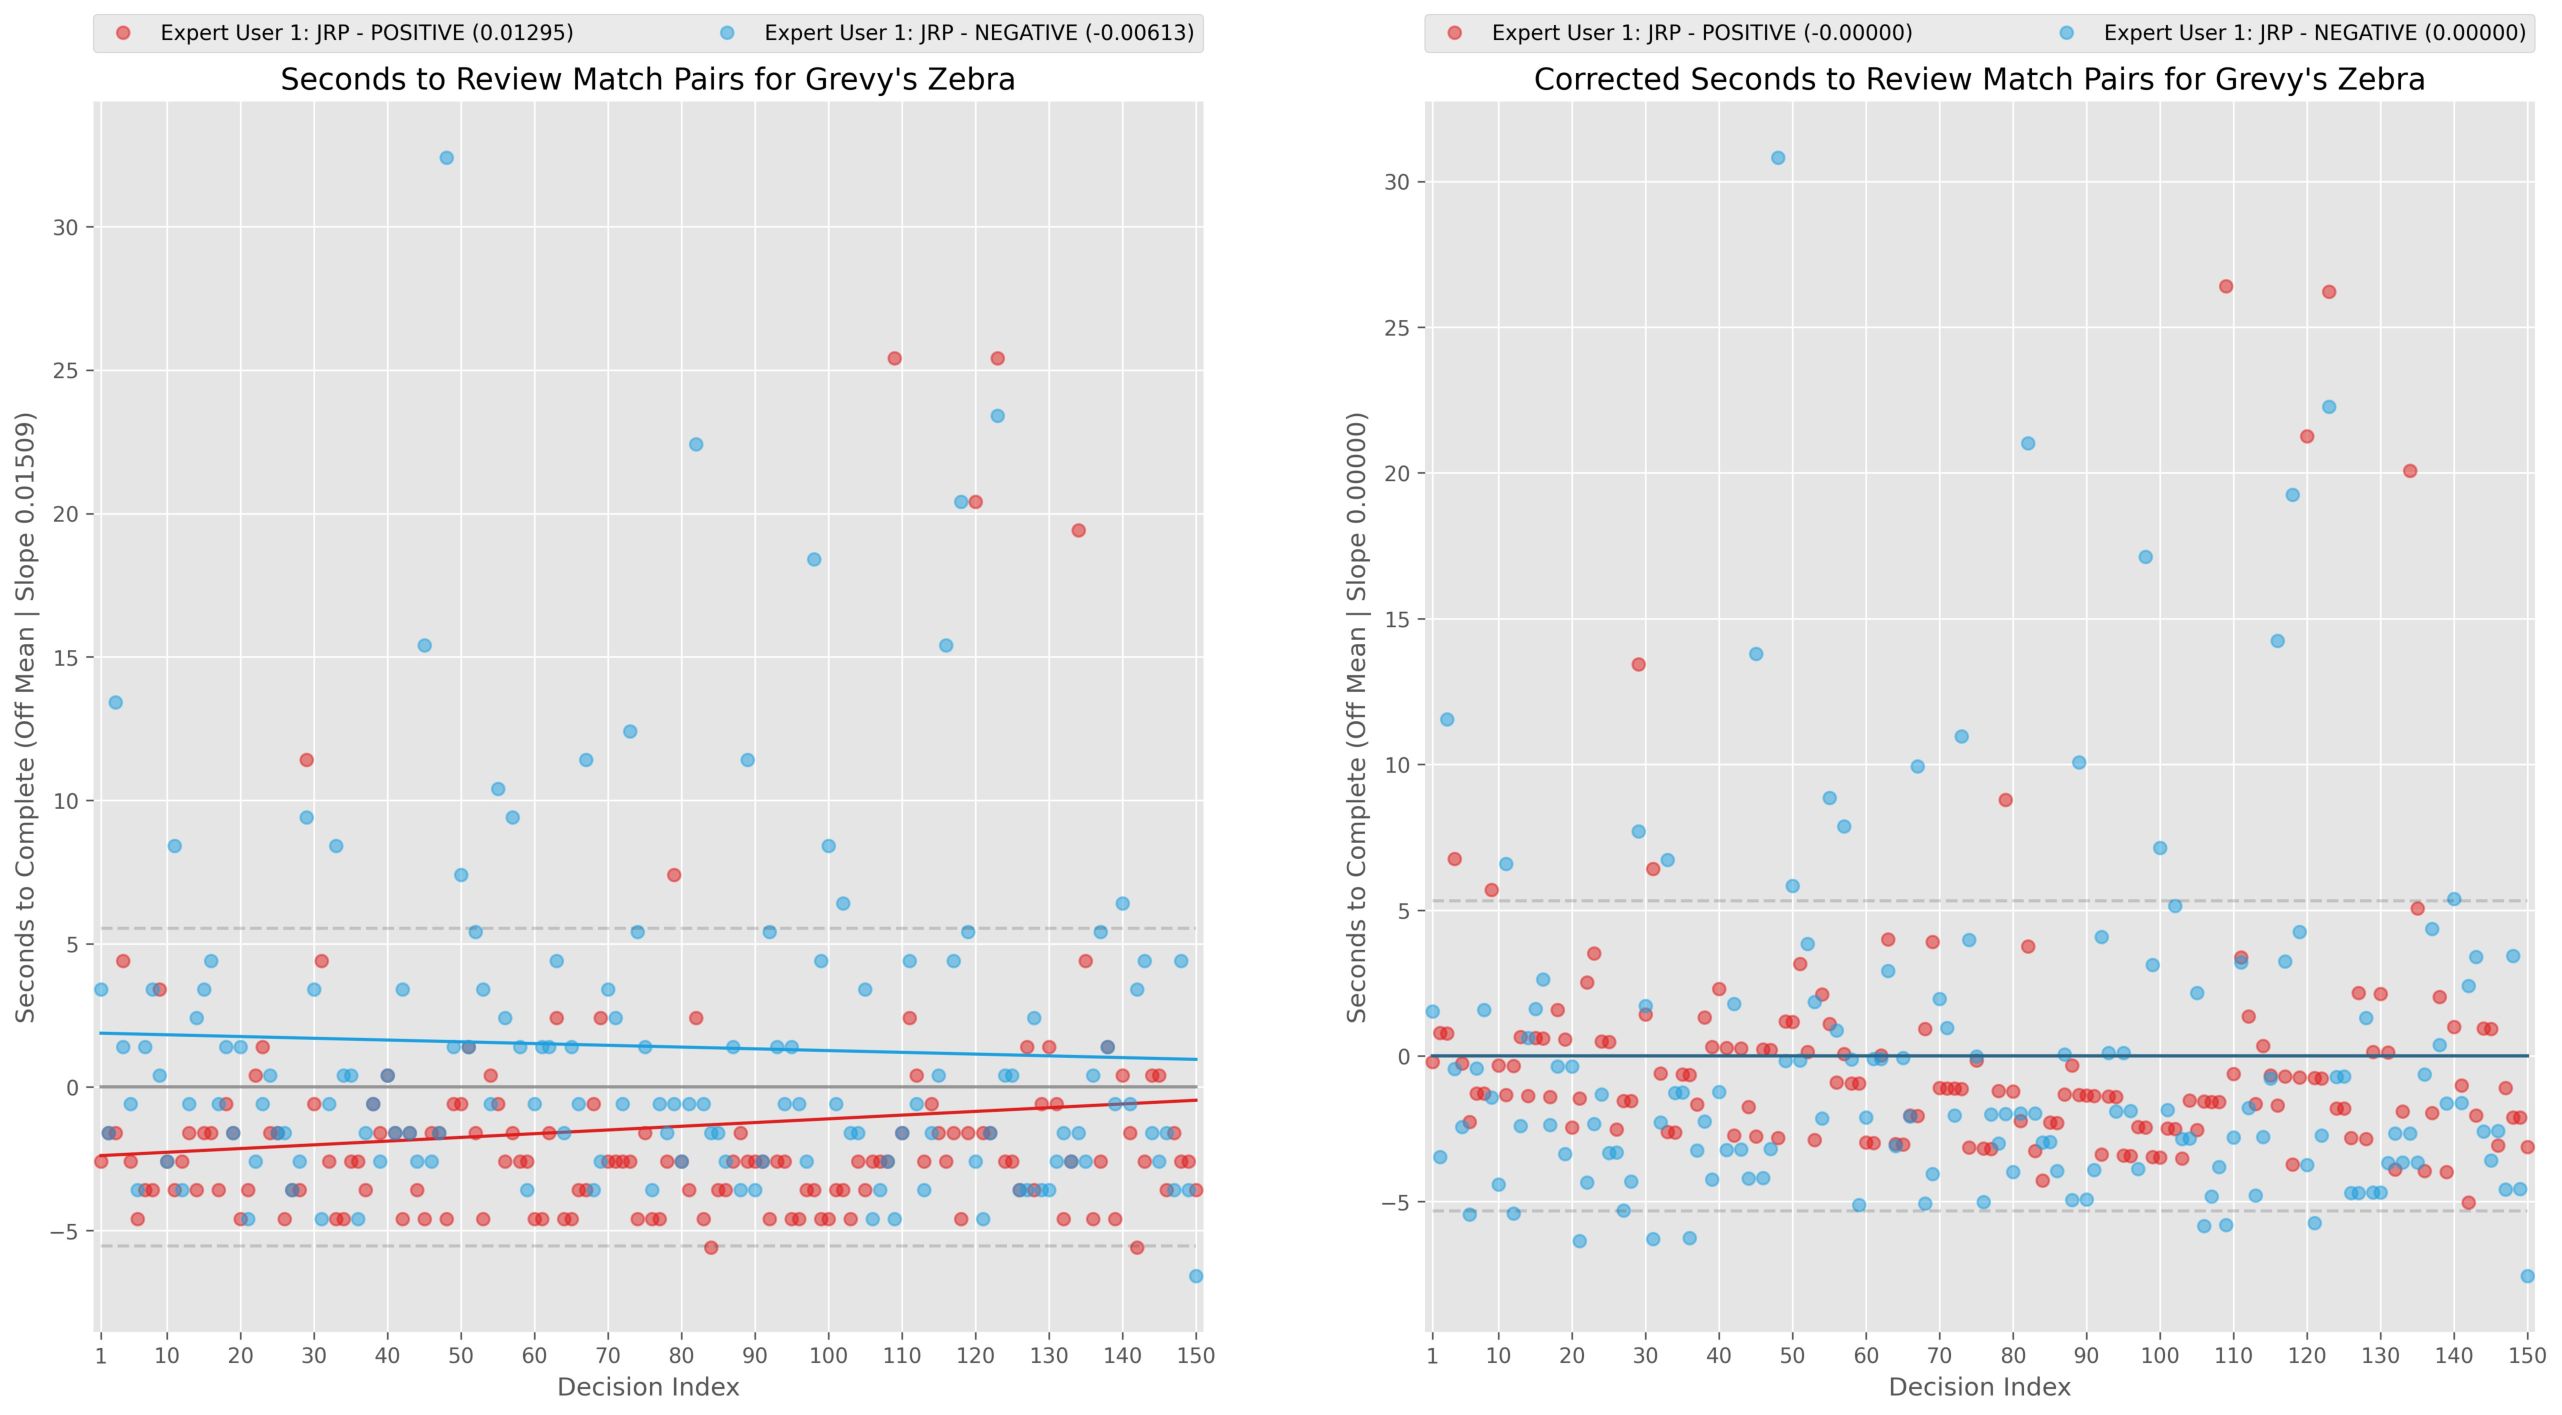
\includegraphics[width=0.90\linewidth]{resources/reviewes_jrp.pdf}
        \\
        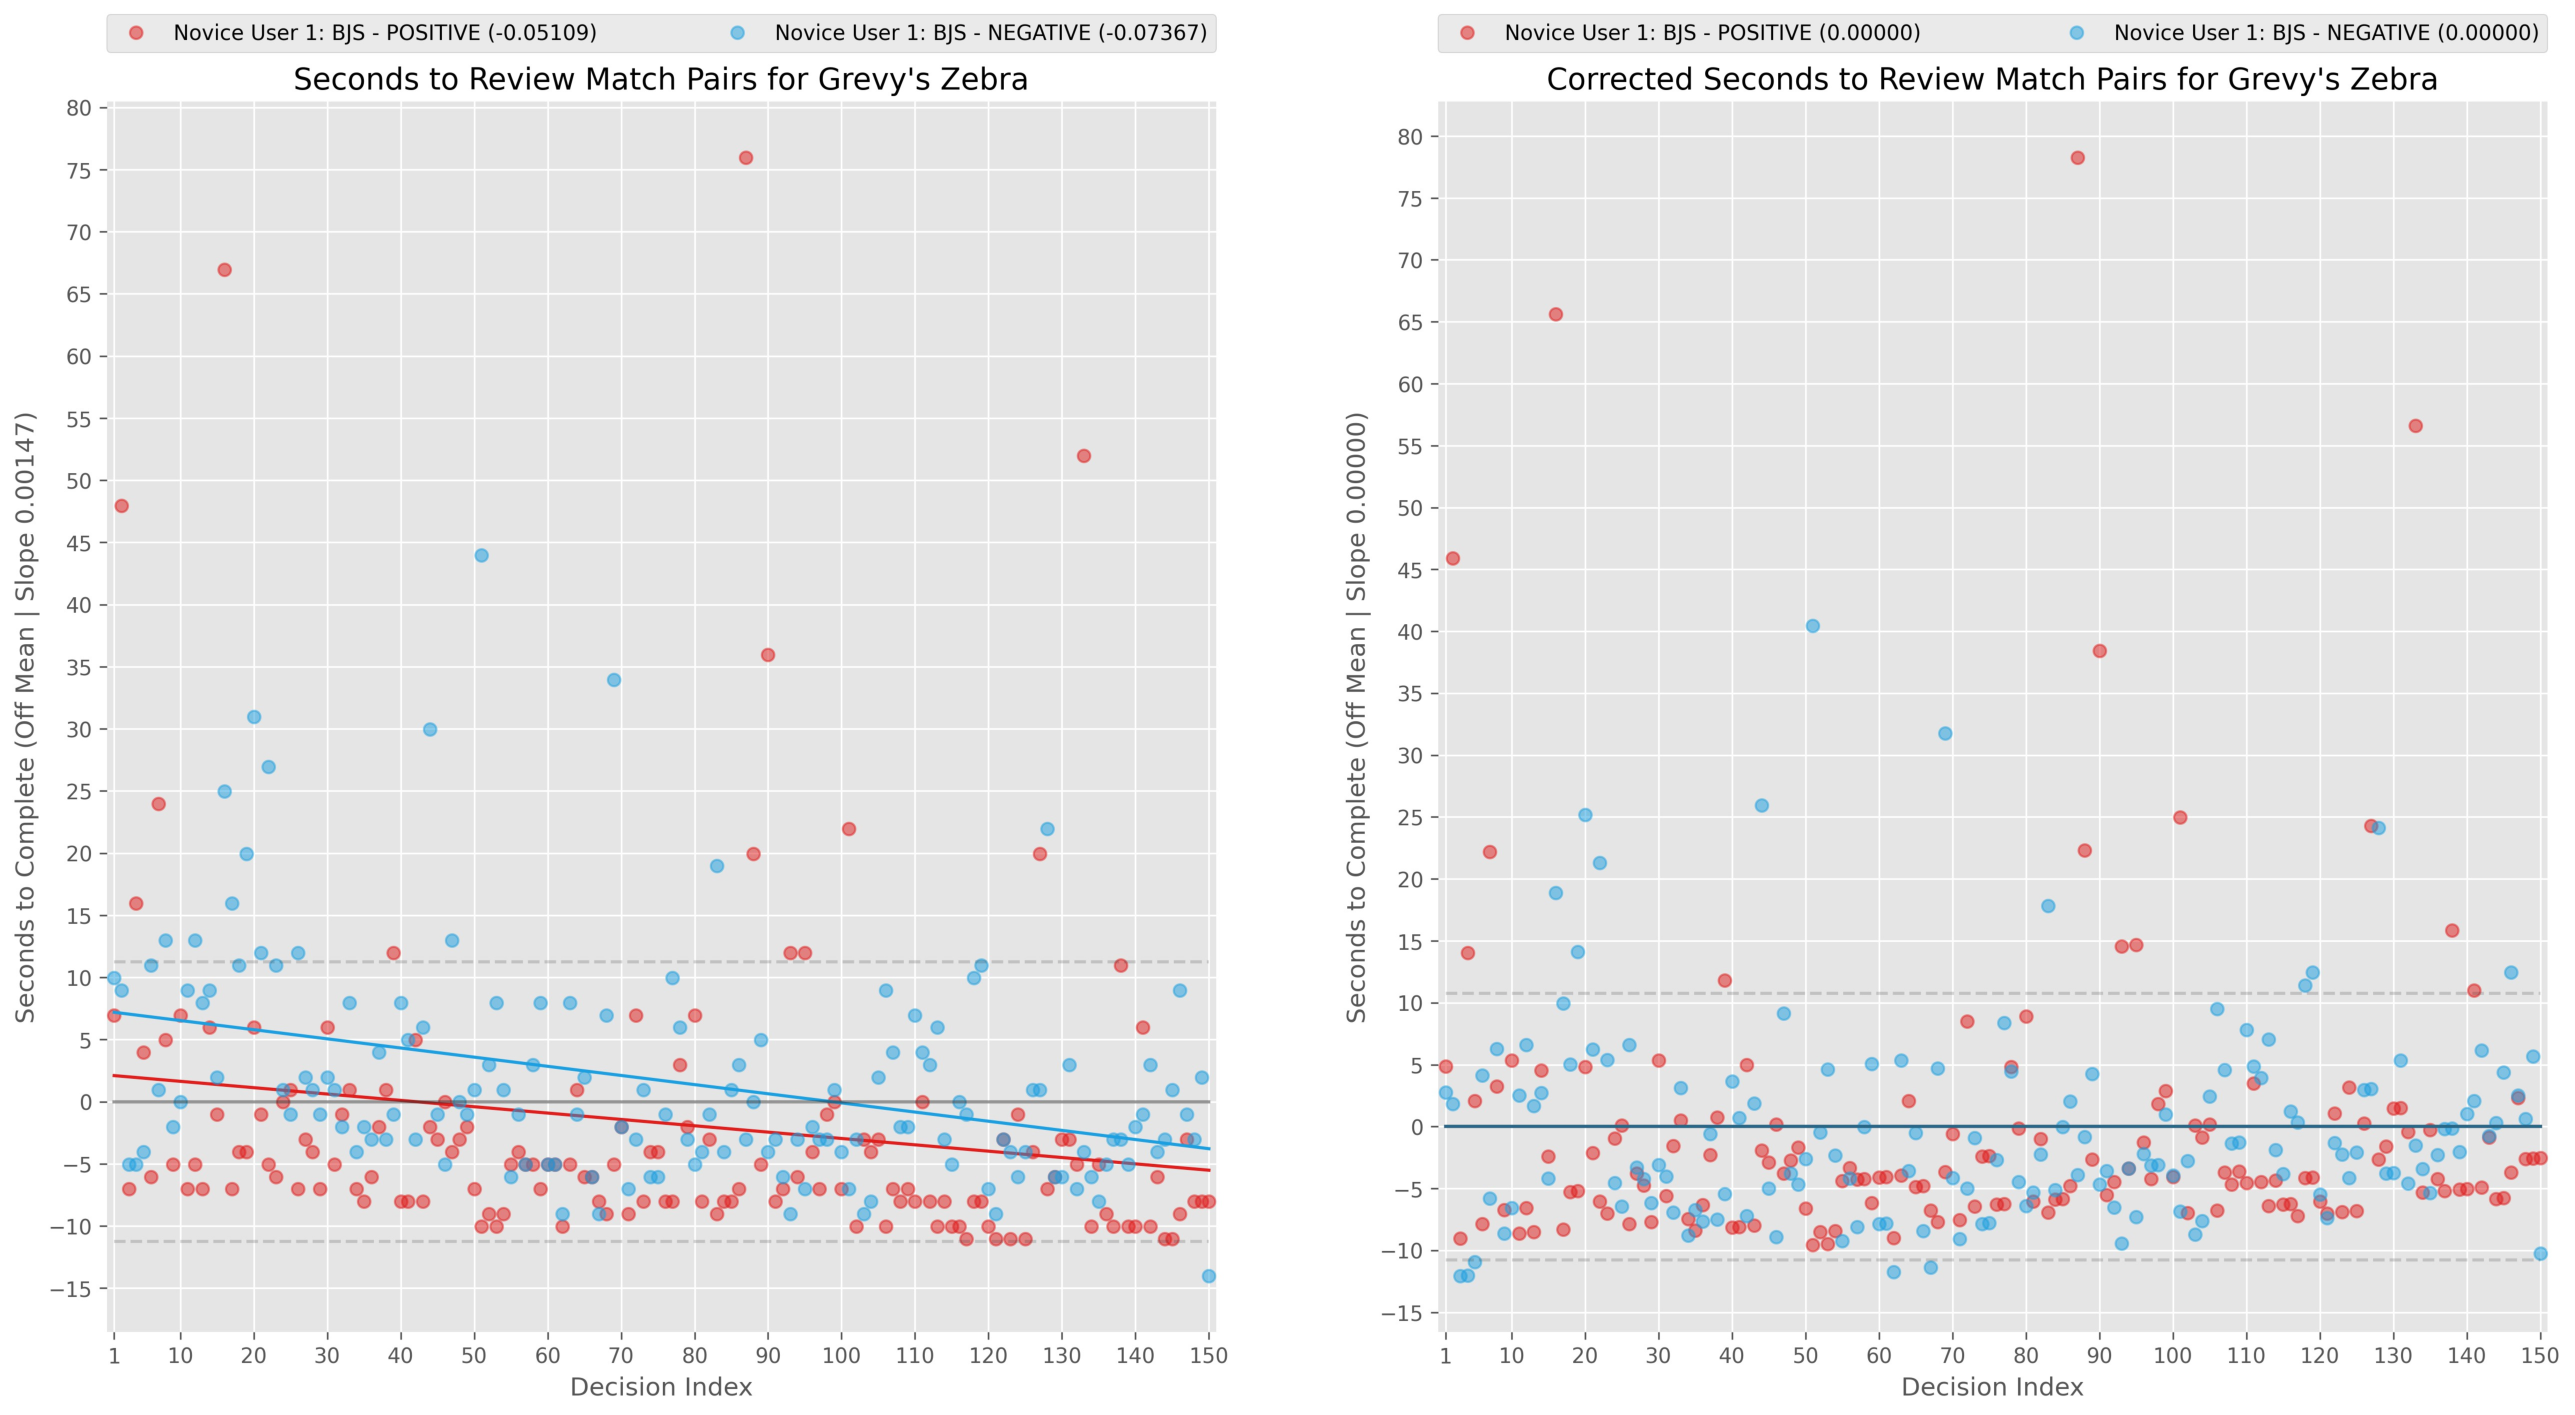
\includegraphics[width=0.90\linewidth]{resources/reviewes_bjs.pdf}
    \end{center}
    \caption{The decision times for various match pairs as seen during the user study.  The ``off mean'' times to complete 150 positive ``same animal'' and 150 negative ``different animal'' match pairs (300 total).  The time for an expert (top) and a novice (bottom) are shown, with the original times (left) and the slope-corrected times (right) displayed for both users.  The positive slope for the expert's ``same animal'' decisions (red line) indicates that the user slowed down over time for those pairs.  The novice user, in contrast, grew more comfortable with the study as it progressed and was faster for both ``same animal'' (negative blue line slope) and ``different animals'' decisions (negative red line slope).}
    \label{fig:user-study-corrections}
\end{figure}

A user's average decision time for all 300 decisions is subtracted from the time for each decision to counteract the effects of any communication delay.  This correction results in a global mean of 0.0, where faster-than-average annotation pairs have a negative seconds time value and slow pairs have positive time values.  However, additional correction is needed because users became more comfortable with the task as the study progressed.  The users, especially the novice users, were faster in their decision-making towards the end of their participation in the study than at the start.  Furthermore, it is generally easier (and therefore faster) to review negative ``different animal'' pairs because not as many points of comparison are needed to prove two animals are different.  For example, once a user identifies a pattern that does not match, they quickly move on.  To verify a positive match, users tend to be a bit more careful and look for more than one point of comparison, which takes additional time.  For all of the participants -- experts and novices alike -- their 150 positive pair decisions were slower on average than the 150 negative pair decisions.  Two lines were then fit to the ``off mean'' times for positive and negative examples to correct these effects.  The slope of each line was then used to offset the individual times for each decision where the positive and negative mean times were equal to the global mean.  The plots in Figure~\ref{fig:user-study-corrections} show the original and corrected times for an expert (the author, top row) and a novice (bottom row).  The expert was more consistent in their review times (standard deviation 5.5 seconds), while the novice, as expected, was more varied ($\sigma=11.2$ seconds).

\begin{figure}[!t]
    \begin{center}
        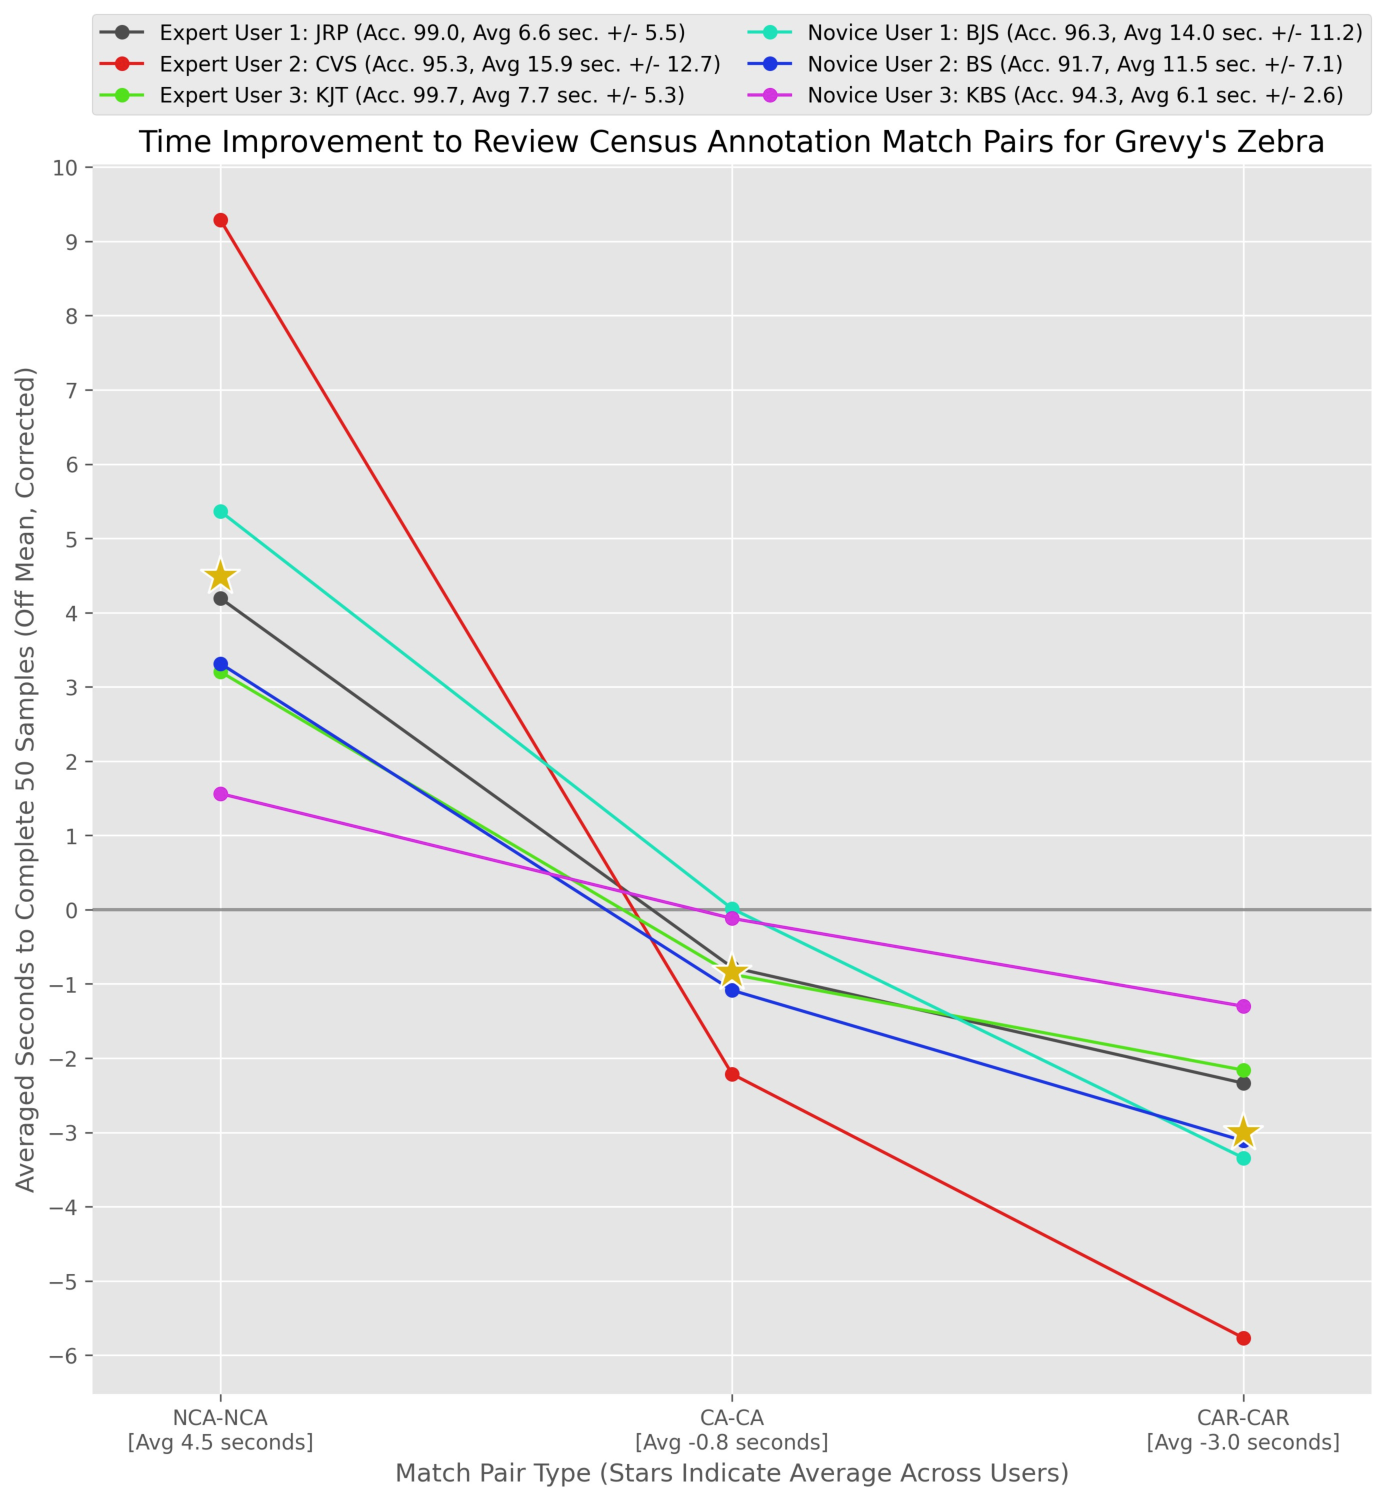
\includegraphics[width=0.70\linewidth]{resources/improvement.pdf}
    \end{center}
    \caption{A comparison of the decision times for each match pair type.  All six users were given 50 match examples between two non-CAs (NCAs), two Census Annotations (CAs), and two Census Annotation Regions (CARs).  The slowest pairs to review were the non-CAs at 4.5 seconds (on average) slower than each user's unique mean.  The fastest pairs to review were the CAR-CAR pairs, with an average time savings of 3.0 seconds per decision.}
    \label{fig:user-study-improvement}
\end{figure}

After each user's decision times are corrected with their own unique global mean and calculated slope offsets, the relative time spent reviewing NCA-NCA, CA-CA, and CAR-CAR pairs can be calculated and compared.  Each user was shown 50 examples (25 positive, 25 negative) of each category during the user study, randomly interlaced with the other types and combinations of pairs.  Figure~\ref{fig:user-study-improvement} shows the off-mean times each user spent on each match pair type.  We can see that NCA-NCA pairs were significantly slower for all users than their mean decision times.  On average, each user spent 4.5 additional seconds on these pairs, indicating they were more challenging to review. On the other hand, match decisions between CA-CA pairs were much improved and were faster than the average by 0.8 seconds.  Importantly, each user was as fast as their average decision time with CAs or was noticeably faster.  Lastly, match pairs between two CARs were substantially faster, saving 3.0 seconds on average per decision.  As for accuracy, the expert reviewers had an average accuracy of 98\% compared to the novice users, who averaged at 94.1\%, with the lowest individual accuracy of 91.7\%.

\begin{figure}[!t]
    \begin{center}
        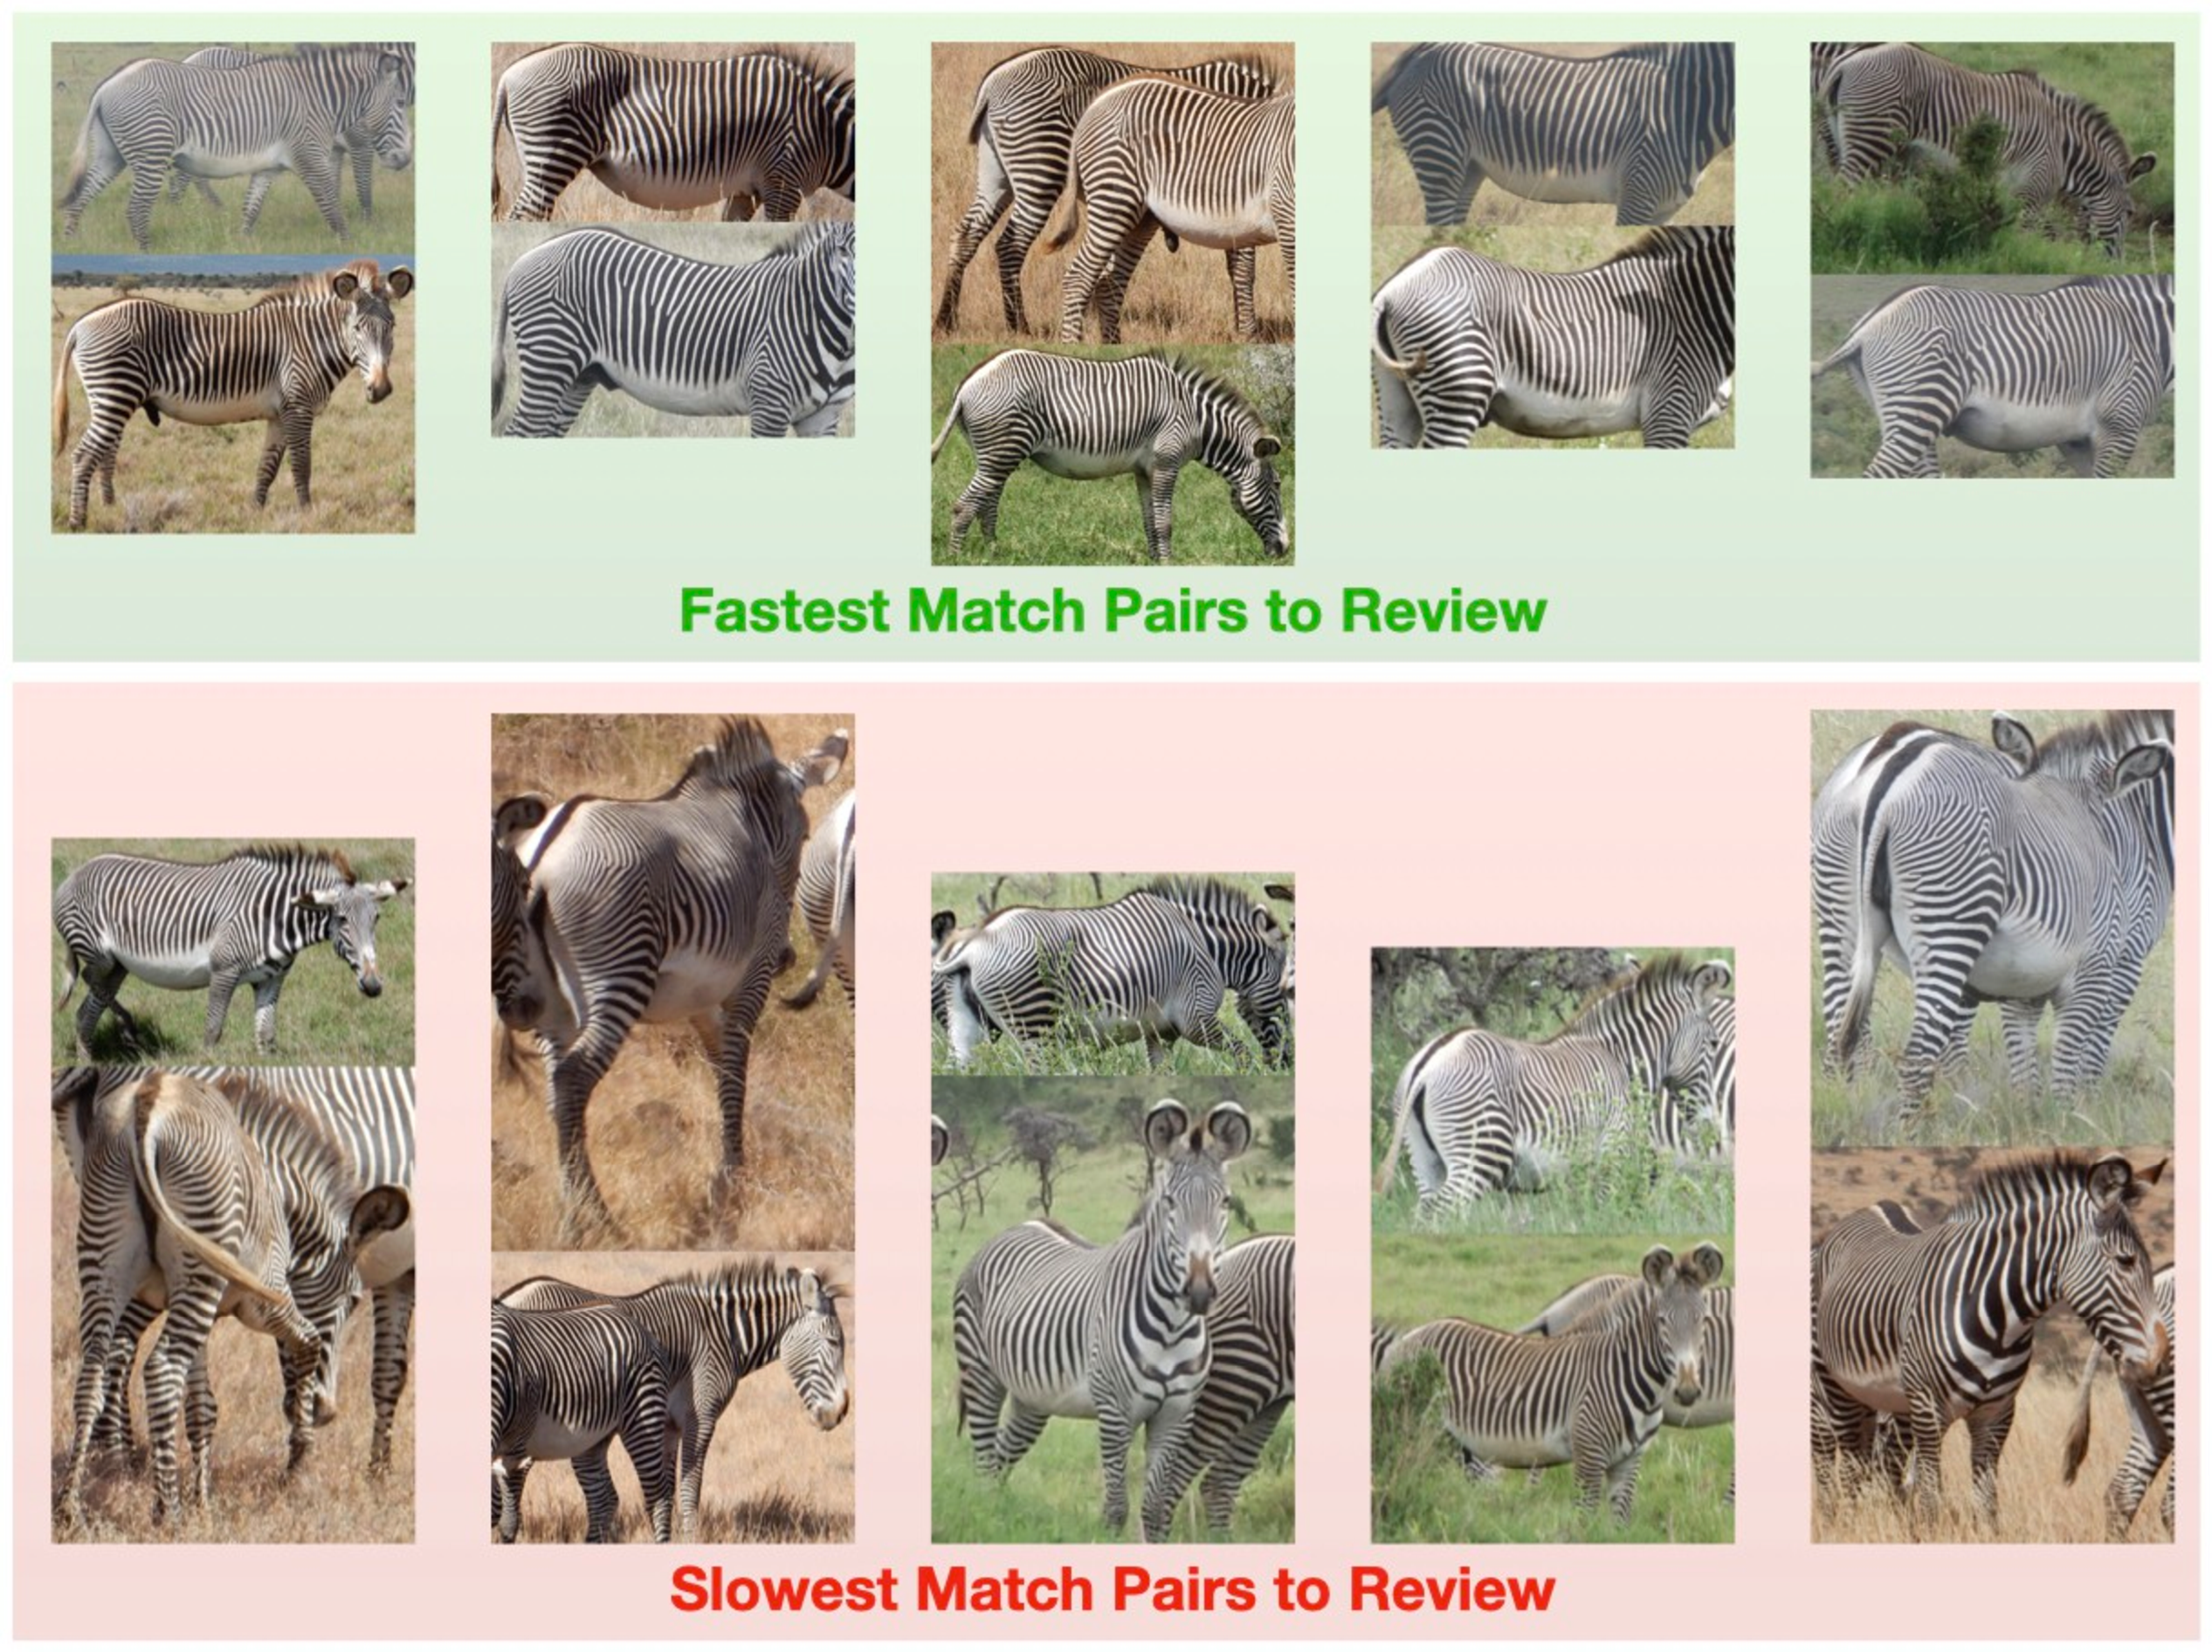
\includegraphics[width=0.90\linewidth]{resources/user-study-pairs.pdf}
    \end{center}
    \caption{Example images of the fastest and slowest match pairs during the user study.  Out of the 300 match pairs in the user study, the five annotations that users spent the most time on (slowest) and the five annotations that users spent the last time (fastest) are shown.  We can see that the slowest match pairs to review have very hard to compare viewpoints and visual information that is obscured.  The fastest annotations show clearly at least one of the two comparable regions for Gr\'evy's zebra Census Annotations, with two of the fastest five matches being CAR-CAR pairs.}
    \label{fig:user-study-pairs}
\end{figure}

Let us now consider a photographic census where only comparable annotations are used but no other restrictions on quality are applied.  Let us also assume that any human review needed during ID curation is an unbiased collection across the 12 match pair types from above.  The results from the user study suggest that the average rate of decisions for all users is approximately 400 decisions per hour per user and an accuracy rate of 96.1\%.  If we consider a photographic census constructed out of only Census Annotation Regions, the decision throughput increases to 560 decisions per hour, a 40\% relative speed improvement.  Furthermore, the study users made 71 decision errors, and 52 of those errors were with pairs that contained at least one NCA.  If NCAs are excluded from ID curation, the number of errors made by the human verifiers would have been reduced by 73.2\%.  Lastly, we can compare the match pairs on which the study users spend the least amount of total (off mean) time against the pairs they spent the most combined time on.  Figure~\ref{fig:user-study-pairs} shows the five fastest and five slowest pairs, which clearly shows that CAs and CA Regions are a strong indicator for how easy and quickly annotation pairs can be reviewed by humans.

While the impact on human decision-making is vital to analyze, it is not the only photographic censusing process that decides match pairs.  Automated verifiers are used extensively during ID curation as the desired replacement for human reviewers, and the impact of CA and CA-R represents a substantial opportunity to improve automation.  Now that CA-Rs have been shown to dramatically improve human verification performance and decision times, we need to analyze what improvements they may have with automated match verification.

\section{Analysis on Separability of Automated Decisions}

VAMP is a verification algorithm developed by Crall~\cite{crall_identifying_2017} that decides if pairs of annotations are one of three mutually-exclusive states: 1) ``same animal'' (\textit{match}), 2) ``different animals'' (\textit{nomatch}), or 3) ``cannot tell'' (\textit{notcomp}; representing an incomparable decision).  We would like to determine 1) how well the algorithm performs on held-out validation data with different types of annotation pairs and 2) how separable are the score predictions between positive and negative pairs.  A collection of three VAMP models was created with the extensive ground-truth pair decisions provided by the GZCD.  Each VAMP model is a set of cross-validated random forest (RF) classifiers trained on a fixed set of pairs mined from the animal ID database.  The three VAMP models are defined by the annotations and match pairs on which they were trained.  The following models were generated using all of the named annotations in the GZCD ID database (for a range of qualities):

\numsquishlist
\item Named Annotations - 20,046 pairs for 5,281 annots.
\item Census Annotations - 14,493 pairs for 4,142 annots.
\item CA Regions - 14,320 pairs for 4,142 annots.
\numsquishend

Each model was validated for a fixed False-Positive Rate (FPR) of 1\% and automated decision thresholds for \texttt{match} (same animal) and \texttt{nomatch} (different animals) were selected.  Encouragingly, the ``Named Annotations'' VAMP model performed similarly to previous Gr\'evy's zebra VAMP models trained on past censusing events for that species and used \texttt{match/nomatch} decision thresholds of 0.8062 and 0.8538, respectfully.  These thresholds are used, for example, in the Graph ID algorithm to decide if a given annotation pair can be automatically reviewed.  For comparison, a VAMP model trained on good-quality right-side Gr\'evy's zebra annotations during the GGR-18 used thresholds of 0.7732 and 0.8605, respectively.  In cross-validation, the model automatically decided 15,921 out of 20,046 of the pairs (79.4\% automation).  For \texttt{match} decisions, the model correctly decided 7,294 out of 8,717 pairs (84\%) and 7884 out of 10460 \texttt{nomatch} decisions (75\%).  Since these annotations include non-CAs, the model predicts a third option for ``notcomp'' (an incomparable match).  With a simple threshold of 50\% (due to low relative volume of examples), the model automatically classified 355 out of 869 pairs (41\% automated) but made 181 errors in the process (FPR 34\%).

The CA and CA Region VAMP models were trained on fewer ground-truth pairs (14,493) than the ``Named Annotations'' model.  However, this is an expected reduction as the total number of annotations decreased significantly from 5,281 to 4,142. The average number of reviews per CA is lower at 3.5 compared to the global mean of 3.8 reviews.  The CA VAMP model was also configured to optimize for an FPR of 1\% during cross-validation and has a much lower \texttt{match} automatic decision threshold.  The model uses 0.6291 and 0.8695 for \texttt{match/nomatch} decisions and was able to automate 13,014 out of 14,493 decisions (89.8\% automated) in total.  This increased level of automation is not surprising as the VAMP model is only being given annotations that should be confidently decidable, as per the design of Census Annotations.  The level of automation allows for 6,069 out of 6,540 \texttt{match} decisions to be automated (93\%) and 6,801 out of 7,848 for \texttt{nomatch} (87\%).

\begin{table}[!t]
    \caption{The VAMP decision thresholds for three different sets of annotations.  Three separate VAMP models were trained: 1) Named Annotations, 2) Census Annotations (CA), and 3) Census Annotation Regions (CA-R).  The CA Region model performs the best and offers the highest degree of automation as it provides the cleanest version of each annotation for visual comparison.}
    \label{table:vamp-thresholds}
    \begin{center}
        \begin{tabular}{| l | l | l | r |}
            \hline
                           & \texttt{match}     & \texttt{nomatch}   &                     \\
            \textbf{Model} & \textbf{Threshold} & \textbf{Threshold} & \textbf{Automation} \\
            \hline
            Named [FPR]    & 0.8062             & 0.8538             & 79.4\%              \\
            \hline
            CA [FPR]       & 0.6291             & 0.8695             & 89.8\%              \\
            \hline
            CA-R [FPR]     & 0.5305             & 0.8496             & 94.6\%              \\
            \hline
            CA-R [MCC]     & 0.5000             & 0.5513             & 99.0\%              \\
            \hline
        \end{tabular}
    \end{center}
\end{table}

The CA-R VAMP model is expected to be the most discriminative at its task and, therefore, should achieve the highest levels of automation.  No changes to the underlying name IDs or the number of total pairs for training were made compared to the previous CA VAMP model.  The only change made was using the more focused bounding boxes around the identifying information for the Gr\'evy's zebra and training VAMP on only those regions.  The assumption here is that if a human reviewer decided a CA-CA annotation pair as ``same animal'', its associated CA-R to CA-R pair should inherit the same ground-truth decision.  Unfortunately, this process could not work for all ground-truth human decisions, as 173 incomparable decisions could not be inherited.  Any incomparable match decisions were intentionally left out of training as they represented only 1.2\% of the match pairs.  The resulting VAMP model for CA Regions, as expected, performs very well.  Automated thresholds were selected for \texttt{match} and \texttt{nomatch} at 0.5305 and 0.8496, again using a FPR of 1\%.  This model allowed for automated decisions for 13,552 out of 14,320 pairs (94.6\% automation).  For \texttt{match} decisions, 6,236 out of 6,461 of the pairs were automatically decided, an outstanding level of automation at 97\%.  Likewise for \texttt{nomatch}, the model was able to decide 7,173 out of 7,753 pairs (93\%).  A summary of all three models, their decision thresholds, and their levels of automation can be seen in Table~\ref{table:vamp-thresholds}.

Furthermore, suppose the best CA Region VAMP model's thresholds are selected to optimize the classification task's Matthews Correlation Coefficient (MCC). In that case, the thresholds can be lowered even further to 0.5 (the lowest allowed) for \texttt{match} and 0.5513 for \texttt{nomatch}.  These thresholds result in more errors overall and a higher level of automation as 14,182 out of 14,320 pairs are automatically decided (99.0\%).  To achieve this level of automation, 90 out of 6,340 (1.4\%) \texttt{match} decisions are made incorrectly while 230 out of 7,842 (2.9\%) \texttt{nomatch} decisions are incorrect (total FPR of 2.3\%).  For comparison, the ``Named Annotation'' model can also be tuned with the MCC to automate 96.9\% of decisions but unfortunately has an overall FPR of 6.3\% (5\% for \texttt{match} and 7\% for \texttt{nomatch}).

In summary, the ability of the CA Region VAMP model to quickly and accurately classify pairs reduces the need for human review during a photographic census.  However, even with highly accurate automated verifiers, incidental matching can still be a problem for photographic censusing.  The hope is that using Census Annotation Regions drastically reduces the number of inappropriate matches between annotations, which we will explore next.

\section{Impact on Incidental Matching}

As discussed in Chapter~\ref{chapter:overview}, the matching scenarios that are a significant source of error -- and require human-in-the-loop review -- are photobombs, mother-foal matches, and scenery matches.  The problem is that automated matching between two annotations can sometimes be incorrect and match inappropriate visual information.  Furthermore, incidental matching makes it difficult to accurately separate the rankings between true positives and negatives, hindering our ability to use decision thresholds.  For example, scores for photobombs are hard to distinguish from correct matches because the ranking algorithm is correctly finding corresponding visual information.  The solution to this problem is to remove the ability for distracting background information to match in the first place.  Census Annotation Regions help mitigate the effects of incidental matching because it actively reduces the information within an annotation to only what is used to compare and contrast two annotations.

The GZCD contains many animal IDs and offers an extensive collection of match decisions made by hand; out of 43,048 human reviews, 1,540 were marked as explicitly showing a photobomb, and 1,007 pairs were labeled as a scenery match.  Unfortunately, ground-truth match data on mother-foal photobombs were not collected during the ID curation of GZCD.  However, this chapter's remaining discussion provides examples of mother-foal errors by the LCA algorithm and analyzes the positive impact of using Census Annotation Regions for ID curation.

\subsection{Photobombs}

The GZCD ground-truth match decisions contain 1,540 photobomb pairs, with 239 pairs containing the same ground-truth ID (positive pairs) and 1,301 showing different animals (negative pairs).  We would expect the vast majority of photobomb pairs to be negative decisions -- indeed, it is 84.5\% of the pairs -- but it is not exclusively negative match decisions.  For example, two annotations could have matched from a more distinctive background animal, but the primary animal in both annotations is the same individual.  The candidate set of annotations was filtered to compare the Quality Baseline (defined in Section~\ref{sec:ca-sims}) set from previous sections to the set of CAs and their CA Regions.  The Quality Baseline concerns 764 photobomb pairs, while the two CA algorithms filter out some of those to keep 592.

\begin{figure}[!t]
    \begin{center}
        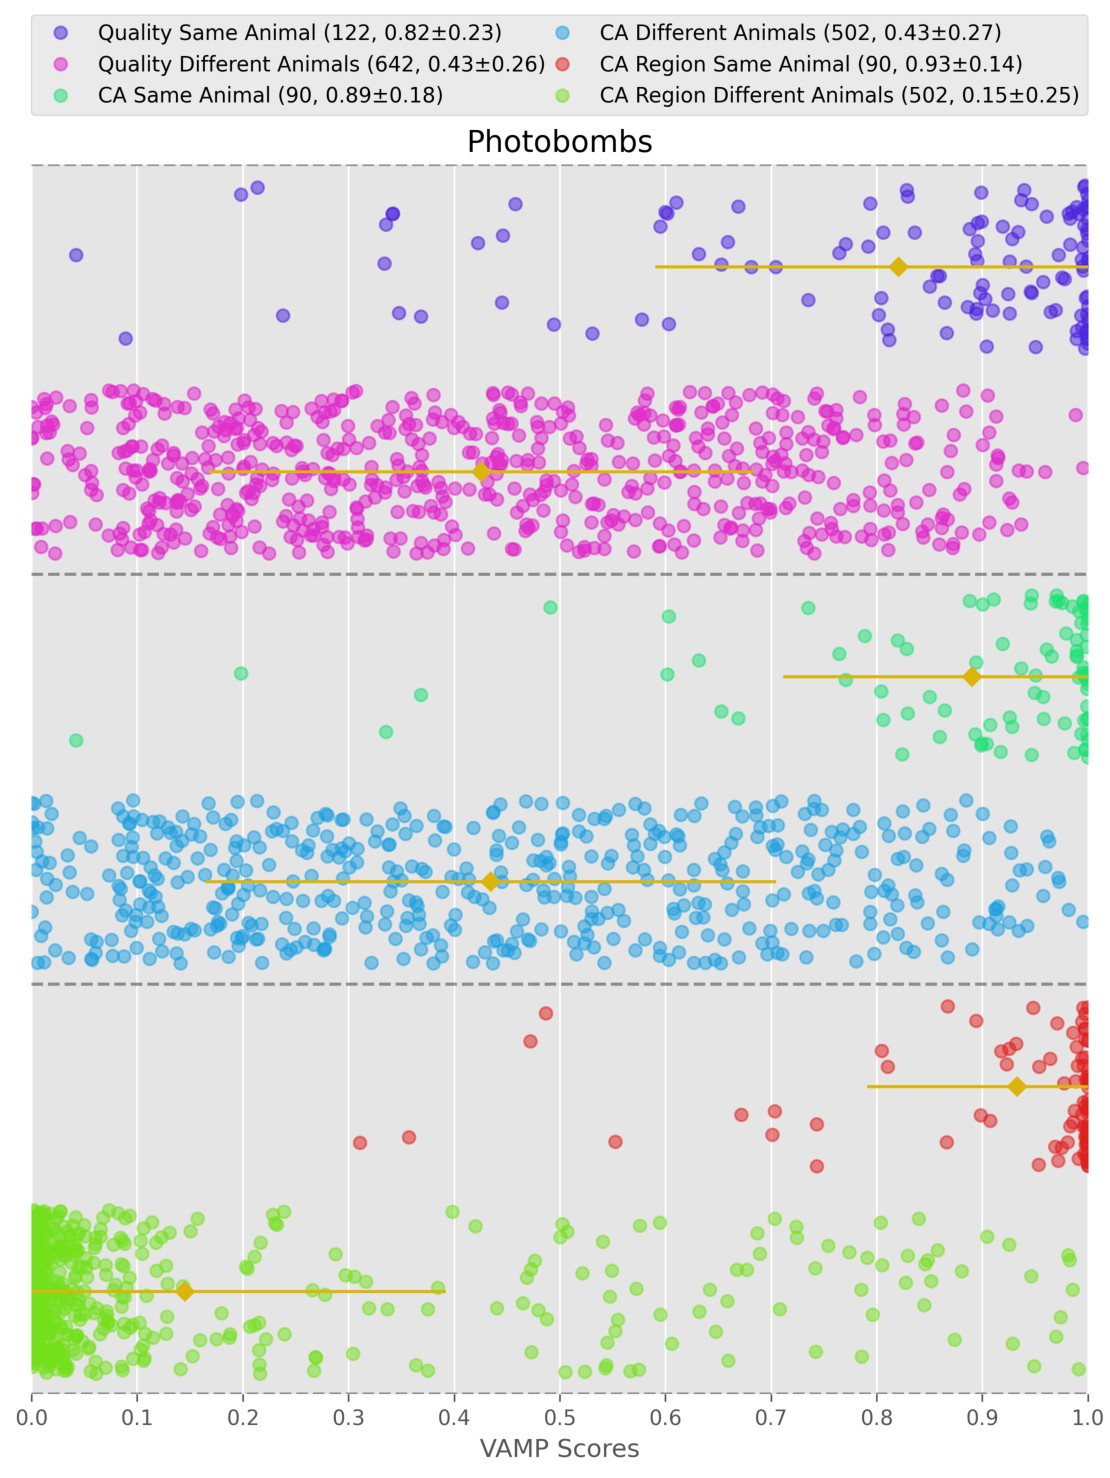
\includegraphics[width=0.48\linewidth]{resources/vamp-incidental-2.pdf}
        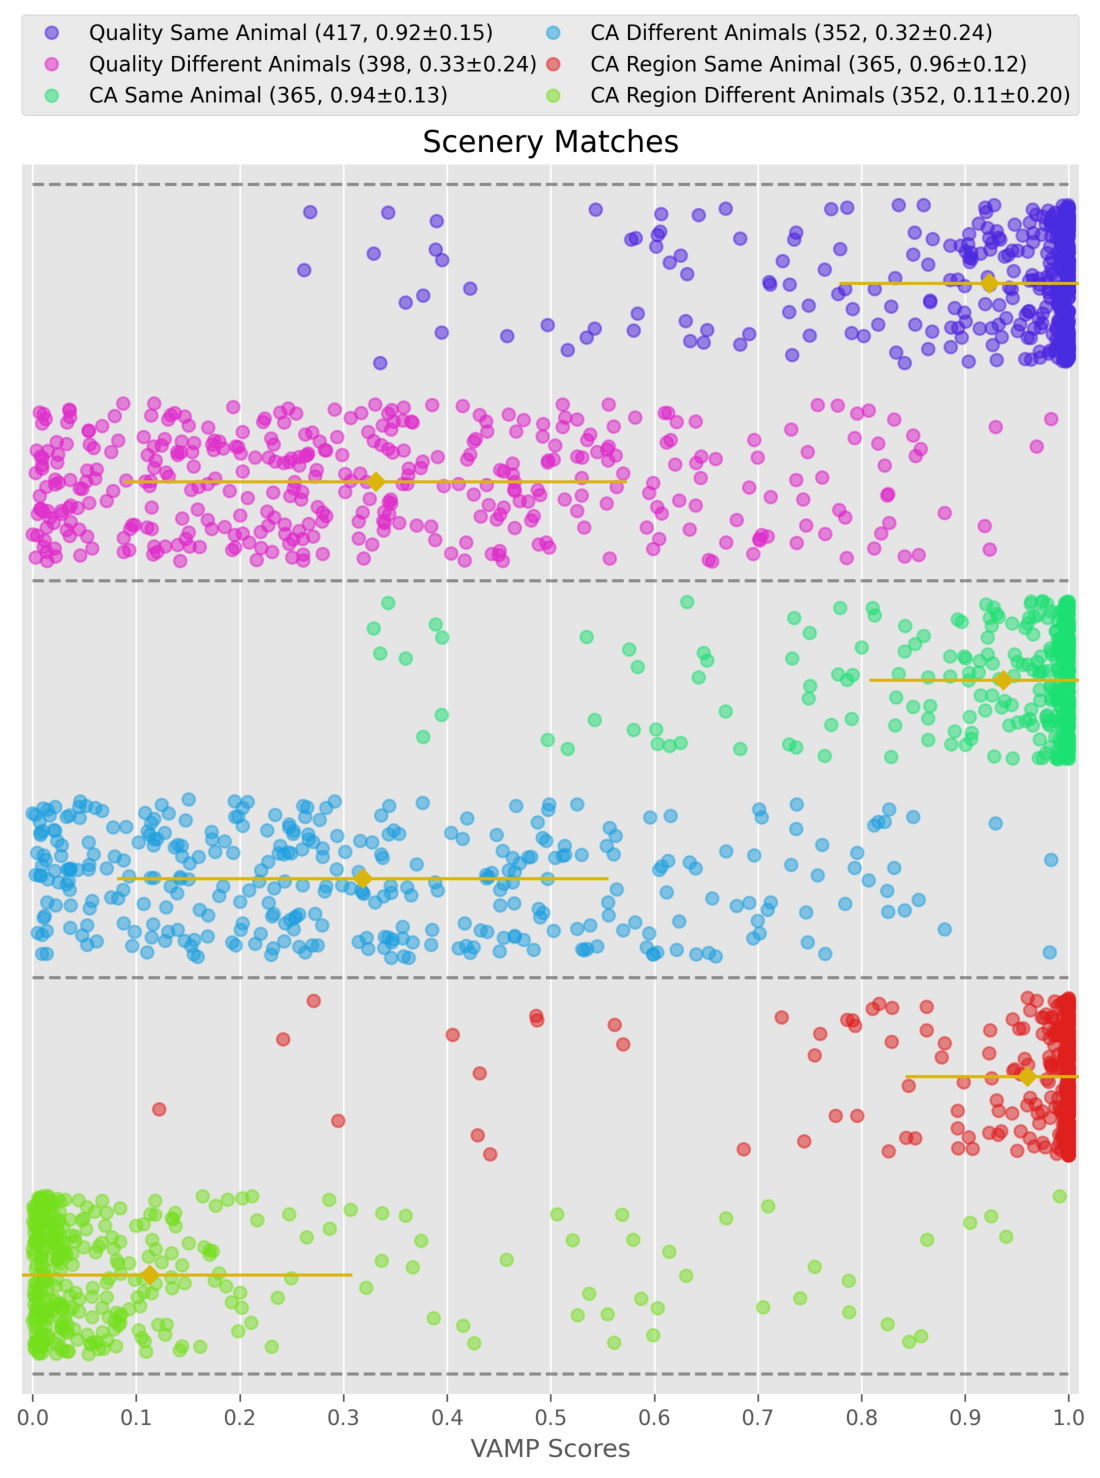
\includegraphics[width=0.48\linewidth]{resources/vamp-incidental-1.pdf}
    \end{center}
    \caption{A scatter plot of the VAMP scores and their separability for three datasets.  The benefit of using Census Annotation Regions over traditional annotations is that it limits the area that is matching to only the identifying information on the body of the animal, decreasing the chance of a photobomb (left) and scenery match (right). The separability of photobomb match scores dramatically improves when Census Annotation Regions (bottom section) are used, with positive pairs scoring 93\% and negative pairs scoring 15\% on average.  Scenery matches also see a dramatic improvement, with positive CA-R pairs scoring 96\% and negative pairs scoring 11\%.}
    \label{fig:vamp-photobomb-scenerymatch}
\end{figure}

Figure~\ref{fig:vamp-photobomb-scenerymatch} (left) shows the VAMP confidence scores for positive and negative ground-truth pairs.  The scores are displayed and separated randomly on a scatter plot simply for easier viewing.  It is clear from looking at the quality baseline for ``different animals'' that there is extreme confusion.  The average VAMP score for these negative pairs is 43$\pm$26\% and appears to be fairly uniform.  Likewise, the Census Annotation scores are not better for ``different animals'' with practically the same average of 43$\pm$27\%.  However, for CA Regions, the VAMP scores are much lower with an average of 15$\pm$25\% and are clustered closer together.  The positive ``same animal'' examples improve slightly from 82$\pm$23\% with the Quality Baseline to 89$\pm$18\% but improve by over 10 points to 93$\pm$25\% with Census Annotation Regions.  By setting a decision threshold at 50\% for VAMP, the Quality Baseline would classify 64.7\% of the pairs correctly, CA with 63.5\%, and CA Regions at 88.3\% accurate.  Picking an optimal operating threshold that maximizes all accuracy for each annotation set yields: Quality Baseline (OP 89\%, accuracy 91.1\%), CA (OP 94\%, accuracy 92.1\%), CA Region (OP 86\%, accuracy 95.8\%).  These results indicate that photobomb cases are 1) significantly reduced in quantity by CA filtering and 2) substantially easier to classify correctly when Census Annotation Regions are compared.

\begin{figure}[!t]
    \begin{center}
        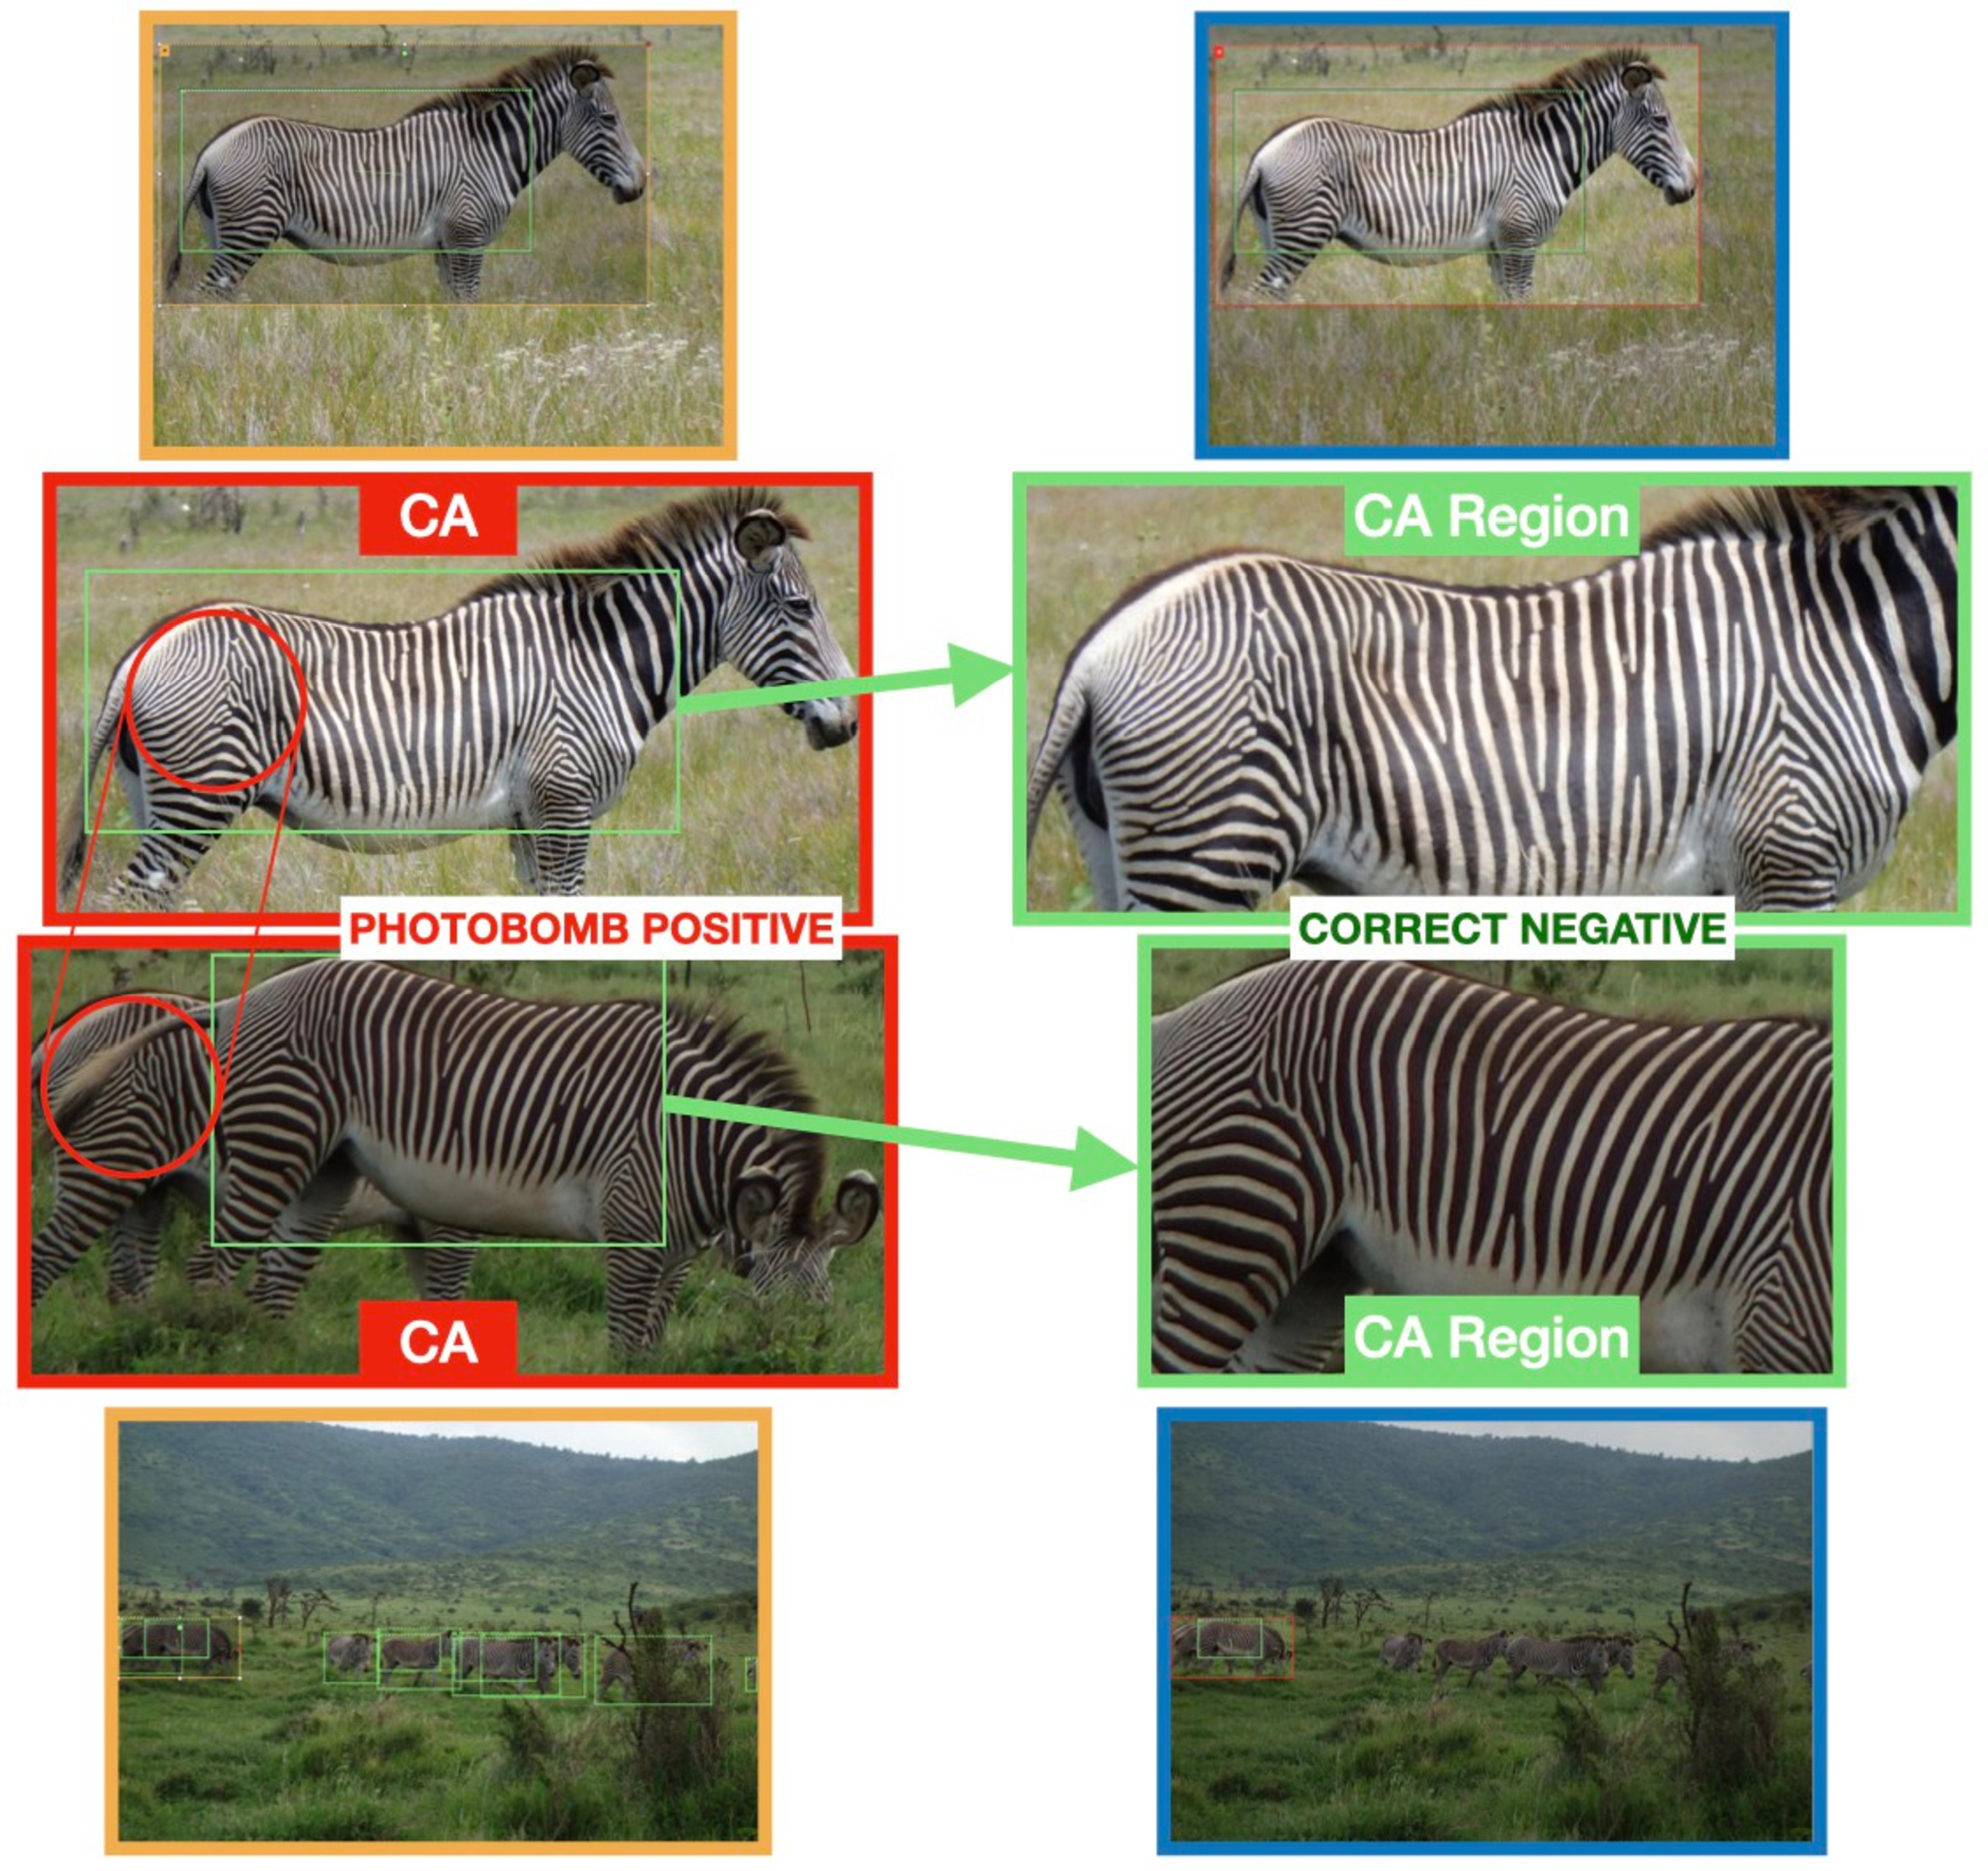
\includegraphics[width=0.7\linewidth]{resources/photobomb-001.pdf}
    \end{center}
    \caption{An example of a photobomb match that is mitigated by using Census Annotation Regions.  The original images (yellow border) with all of the annotations and the highlighted annotation (blue border) matched visually.  The annotations are both Census Annotations (red) but still result in a photobomb (red).  The matched area (red circles) leads to a likely false positive by an automated classifier.  Using the Census Annotation Region (green) shows that the background annotation is removed from visual matching.}
    \label{fig:ca-photobomb-example}
\end{figure}

A real-world example is provided in Figure~\ref{fig:ca-photobomb-example}.  The original images (yellow border) with all annotations and the highlighted annotation (blue border) are matched visually.  The annotations are both Census Annotations (red) but still result in a photobomb because the matched area (red circles) is likely to cause an incorrect ``same animal'' decision.  Instead, when the Census Annotation Regions (green borders) are used, the photobombing annotation is removed from the bounding box and cannot be matched.  The CA VAMP model classifies the photobomb CA pair as 89\% positive (\texttt{match}) whereas the CA Region VAMP model run on the CA Region pair predicts 94\% negative (\texttt{nomatch}).  This example shows that CA alone is insufficient to catch all photobomb errors and provides an example of why a perfect detection -- that captures the tail in its full detail -- is the wrong decision for automating a photographic census with visual ID.

\subsubsection{Mother-Foals}

\begin{figure}[!t]
    \begin{center}
        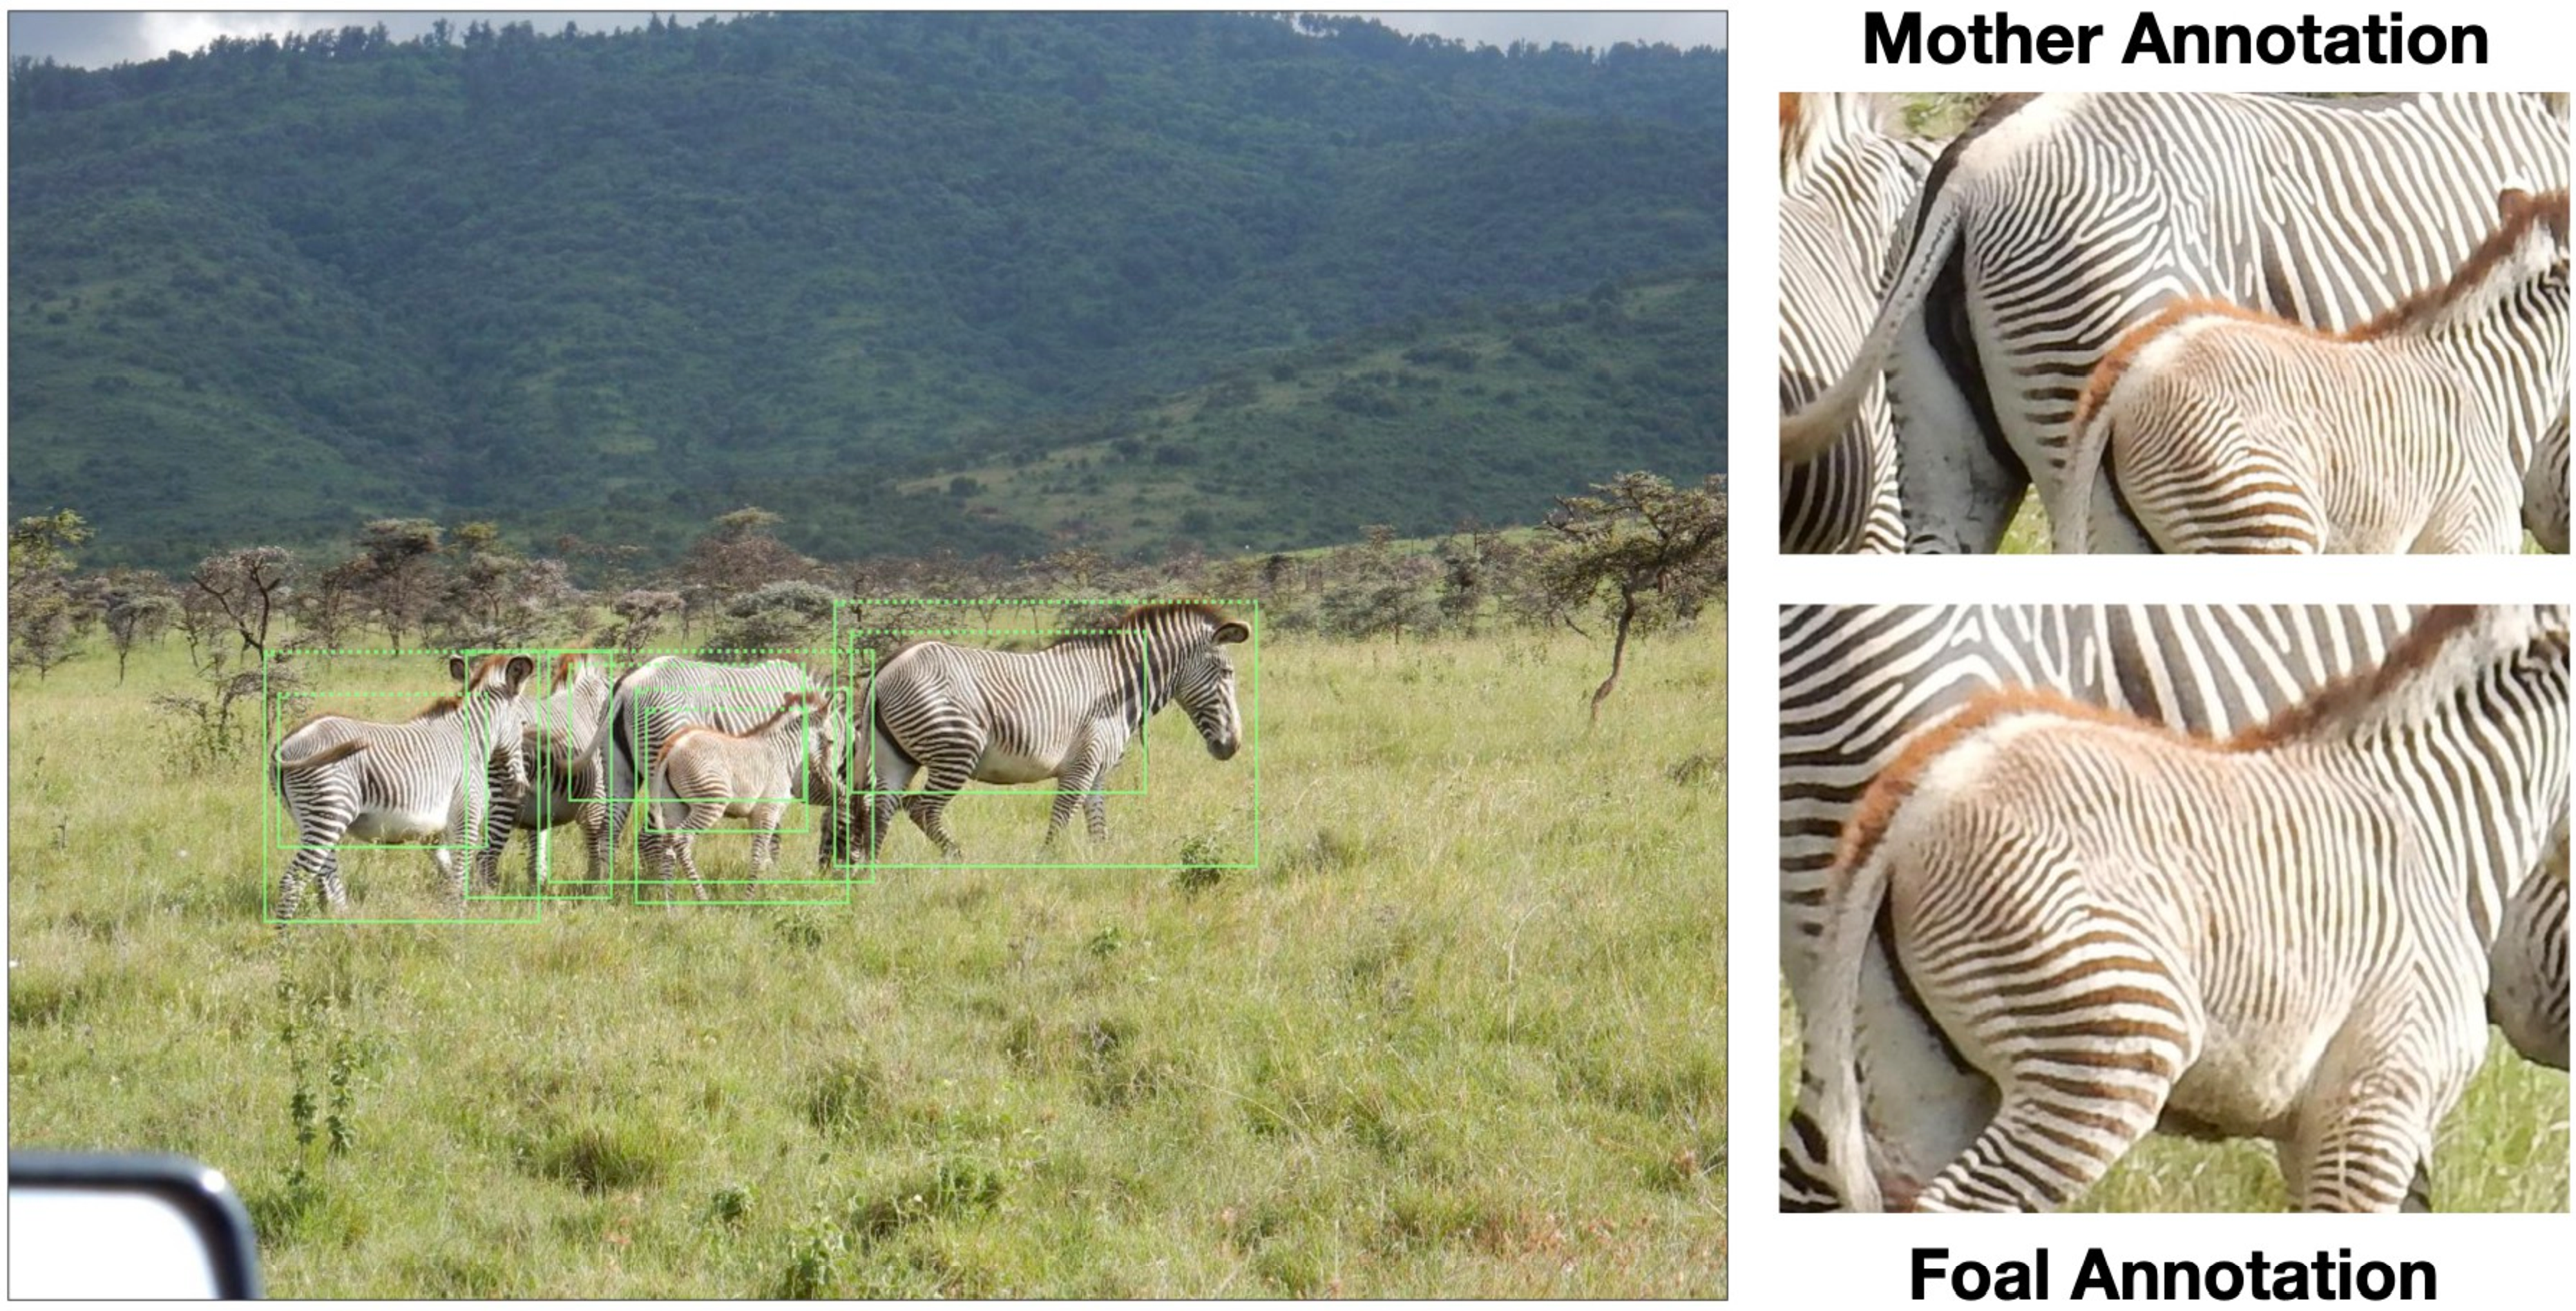
\includegraphics[width=0.9\linewidth]{resources/mother-foal-1.pdf}
    \end{center}
    \caption{An example mother-foal photobomb that was found during the ID curation of the GZCD.  The Census Annotation Regions for a foal and mother overlap significantly and are subsequently incorrectly matched.  All of the annotations for the merged animal ID are reviewed to separate which annotations show the foal or the mother.}
    \label{fig:mother-foal-photobomb-example}
\end{figure}

The human decisions collected by the GZCD did not require explicit labels for mother-foal photobombs when encountered.  When the LCA algorithm was used to identify ground-truth ID errors, however, four animal IDs were found that contained annotations for both a mother and its foal.  This type of ID error indicates that -- at some point during ID curation -- the annotations for the mother and foal were the subject of incidental matching, and their IDs were incorrectly merged.  An example of one of these four ID errors is shown in Figure~\ref{fig:mother-foal-photobomb-example}.  We can see that the Census Annotation Regions for the foal and mother overlap significantly. All annotations for the incorrect animal ID are reviewed by hand to separate which annotations show the foal and which show the mother, generating two new animal IDs as the fix.

To fundamentally mitigate mother-foals photobombs, more advanced and nuanced approaches are needed.  While these techniques are not evaluated here, using an annotation age classifier or an instance segmentation algorithm will help separate highly overlapping sightings like these. However, these methods are not evaluated because the relative frequency of mother-foal photobombs seems to be low (four compared to many dozen identified photobombs during the ID curation of the GZCD) when CA-Rs are used for censusing. In addition, more complex segmentation algorithms will place a high burden on annotating ground-truth pixel data.  In contrast, the impact of scenery matches can be evaluated without more specialized methods and will be discussed next.

\subsection{Scenery Matches}

The GZCD data contains 1,007 scenery match pairs, with 522 pairs containing the same ground-truth ID (positive pairs) and 458 showing different animals (negative pairs).  Since scenery matches are much more random and can happen irrespective of if the match is the same animal or not, a roughly even split is expected (52\% actual).  Scenery matches happen most often when the photographer(s) take pictures within seconds of each other and without moving the camera's field of view, allowing for the background scene to repeat across images.  The annotations were filtered based on the Quality Baseline, using 815 scenery match examples and 717 annotations for the CA algorithms.

As we can see in Figure~\ref{fig:vamp-photobomb-scenerymatch} (right), the 417 ``same animal'' examples for the Quality Baseline are clustered and classified reasonably well with an average prediction of 92$\pm$15\%.  Using Census Annotations improves the classification accuracy slightly to 94$\pm$13\% and even better with Census Annotation Regions to 96$\pm$12\%.  Using the Census Annotations improves positive matches when scenery matches are present, but this case is not where most of the errors originate.  The ``different animals'' matches for the Quality Baseline are much more spread out with an average VAMP score of 33$\pm$24\% and matches the Census Annotation scores at 32$\pm$24\%.  As with photobombs, this is not a surprising failure of the Census Annotation classifier by itself.  Moreover, the number of CAs does not decrease significantly from the Quality Baseline to the CA set, considering the relative matchability of the background textures is separate and independent from the comparability of the foreground animal.  However, Census Annotation Regions significantly improve negative match separability with an average VAMP score of 11$\pm$20\%.  By repeating the exercise from the photobomb discussion and using a decision threshold of 50\%, the Quality Baseline achieves an accuracy of 86.5\%, 87.9\% for Census Annotation accuracy, and 94.7\% for Census Annotation Regions. Picking an optimal operating threshold that maximizes all accuracy for each annotation set yields: Quality Baseline (OP 83\%, accuracy 91.2), CA (OP 72\%, accuracy 92.9\%), CA Region (OP 71\%, accuracy 96.5\%).  These results indicate that scenery matches cases are 1) \textit{not} significantly reduced in quantity by CA filtering but 2) are significantly easier to classify correctly with Census Annotation Regions.

Lastly, we wish to put all of these preceding Census Annotation results together to simulate its impact on human decision-making.  The use of CA and CA-Rs has been shown to improve the speed of human verification, the separability of automated decisions, and reduce the impact of incidental matching. Thus, the next and final section shows how using CA and CA-Rs with photographic censusing results in a similar population estimate while requiring a lot less work from humans.

\section{Population Estimate Simulations} \label{sec:ca-sims}

The primary motivation of Census Annotations and Census Annotation Regions is to improve the automation of a photographic census.  The discussion has demonstrated that 1) humans spend less time reviewing pairs of CAs and CA-Rs, 2) the scores of the VAMP automated verifier are more separable for CAs and CA-Rs than non-CAs, and 3) the frequency of incidental matching is significantly reduced with smaller CA-R bounding boxes.  We still need to determine if CA and CA-R significantly reduce the number of required human decisions and if this reduction in effort causes any loss of accuracy in the final population estimate.  Human effort is an important metric to track because it directly measures how feasible photographic censusing will be for real-world use and is a consistent method for comparing algorithm configurations.  Furthermore, the discussion in Chapter~\ref{chapter:overview} gave examples of why automated machine learning algorithms introduce errors and how a more comprehensive review can mitigate them -- directly associating an increase in accuracy with an increase in work.  Therefore, we can expect that different algorithms, which may be susceptible to different failure methods, can meaningfully influence the accuracy of a population estimate by changing the total amount of human interaction needed.  This section simulates various photographic censusing configurations and analyzes their respective accuracy as a function of automation.  The simulations use the ground-truth ID data from the GZCD and demonstrate that CA and CA-R reduce the need for human involvement while also producing consistent population estimates.

\begin{table}[!t]
    \caption{The number of annotations, names, singletons for three ID evaluation sets and their GGR-16 and GGR-18 Lincoln-Petersen indices.  The ``Quality Baseline'' set is a traditional filter on species, viewpoint, and quality. In contrast, the Census Annotation (CA) and Census Annotation Region (CA-R) annotation sets (identical numbers below) rely on using a more focused definition of comparability.}
    \label{table:census}
    \begin{center}
        \begin{tabular}{| l | r | r | r | r | r |}
            \hline
            \textbf{Set Name} & \textbf{Annots.} & \textbf{Names} & \textbf{Singletons} & \textbf{GGR-16 L-P} & \textbf{GGR-18 L-P} \\
            \hline
            CA-R              & 4,142            & 468            & 51                  & 366$\pm$27          & 373$\pm$29          \\
            \hline
            CA                & 4,142            & 468            & 51                  & 366$\pm$27          & 373$\pm$29          \\
            \hline
            Quality           & 4,269            & 487            & 62                  & 360$\pm$27          & 399$\pm$29          \\
            \hline
        \end{tabular}
    \end{center}
\end{table}

Before we begin, let us review how the GZCD was constructed (see Section~\ref{sec:ca-dataset} for a full description) because it will be the source of ID data for the following simulations.  The ID database was built from two sets of annotations: 1) annotations that passed a ``species, viewpoint, quality'' filter and 2) annotations that were above a specific CA classification score ($0.001$).  The purpose of combining these two sets was that it provided an extensive collection of easy and hard annotation matches and a real-world example of animal sightings.  The first collection used the ground-truth labels for species (Gr\'evy's zebra), viewpoint (any viewpoint that contained \textit{right}, and quality (\textit{ok} or better) as its filter; these annotations will be referred to as the ``Quality Baseline'' set for simulation.  This set of annotations is critical to distinguish as a comparative baseline because it is representative of the annotation filtering methods used in prior photographic censusing studies (see~\cite{parham_photographic_2015},~\cite{berger-wolf_great_2016}, and~\cite{rubenstein_state_2018}).  The annotations that scored above a Census Annotation (CA) threshold of 31\% (the recommended value for Gr\'evy's zebra) were selected as the second evaluation set for simulation.  Furthermore, each of these CAs were hand-annotated with ground-truth Census Annotation Regions (CA-R), which formed the simulation's third evaluation set of annotations.  In summary, the ``Quality Baseline'' set has 4,269 annotations for 487 IDs (62 singletons), and the CA and CA-R sets have 4,142 annotations for 468 IDs (51 singletons).  Table~\ref{table:census} shows a side-by-side comparison of the three sets that will be used for all simulations below.  The reason the number of ground-truth IDs between these sets is different is quite simple: their respective IDs are generated from slightly different sets and quantities of annotations.  For example, half of the difference in the number of IDs is due to singletons, where there are 11 additional singletons in the ``Quality Baseline'' set compared to the CA and CA-R sets.

Since photographic censusing relies on sampling, the exact number of ground-truth IDs is not very meaningful for a direct comparison.  A better way to contrast different simulated animal ID curation results is to examine the differences in their respective Lincoln-Petersen population estimates.  Recall that the GZCD was constructed with images taken in Meru County, Kenya during the Great Gr\'evy's Rally (GGR) photographic censusing events in 2016 (GGR-16) and 2018 (GGR-18).  The GZCD is a useful dataset for simulating ID curation approaches because it offers two ground-truth population estimates: one for 2016 and a second independent one for 2018.  Reviewing the values in Table~\ref{table:census}, the Lincoln-Petersen index for the ``Quality Baseline'' is 360$\pm$27 in 2016 and 399$\pm$29 for 2018.  The population estimate based on only Census Annotations was 366$\pm$27 for GGR 2016 and 373$\pm$29 for GGR 2018.  Finally, simulations with Census Annotation Regions estimate 366$\pm$27 zebra were within Meru County in 2016 and 373$\pm$29 animals in 2018.  These values will function as the ``targets'' for each of the following simulations, conditioned on their input annotation set.

\subsection{Which Annotations to Select}

Six photographic census events were simulated to measure the impact of how annotations are selected: the Graph ID and LCA algorithms were simulated on the three annotation sets, respectively.  All of the simulations in this sub-section used HotSpotter for the ranking algorithm and VAMP as the automated verifier.  Each decision management algorithm was provided with the same underlying ranked list from HotSpotter.  Hotspotter was configured to use $K=5$, $K_{\text{norm}}=5$, and had spatial verification turned on (as recommended by~\cite{crall_identifying_2017} for Gr\'evy's zebra).  These values control the number of Approximate Nearest Neighbor matches returned for each SIFT keypoint and determine how to normalize their respective match scores.  Furthermore, the ranked list was configured to return the 10 highest-scoring annotations ($n_{\text{top}}=10$) for each sighting.  The ``Quality Baseline'' set used 27,075 pairs from HotSpotter's LNBNN ranking algorithm, and the CA and CA-R sets were provided with 25,831 ranked pairs.  When LCA received these pairs, it re-scored them with its internal weighting function (i.e., the ``weighter'') and predicted 17,862 positive edges for the ``Quality Baseline'' set, 17,205 for the CAs, and 17,749 for CA Regions.  Each of the LCA weighters was initialized using a VAMP~\cite{crall_identifying_2017} model that was trained for each set independently and used the scores for 1,000 randomly sampled \textit{``same animal''} and 1,000 \textit{``different animals''} ground-truth decision pairs.  The LCA simulations were allowed to run to convergence (configured with a minimum delta convergence multiplier of 1.5 and minimum delta stability ratio of 4), but the Graph ID algorithm (configured for a positive redundancy of 2 and a negative redundancy of 1) was stopped prematurely after 20,000 human decisions were requested.

\begin{figure}[!t]
    \begin{center}
        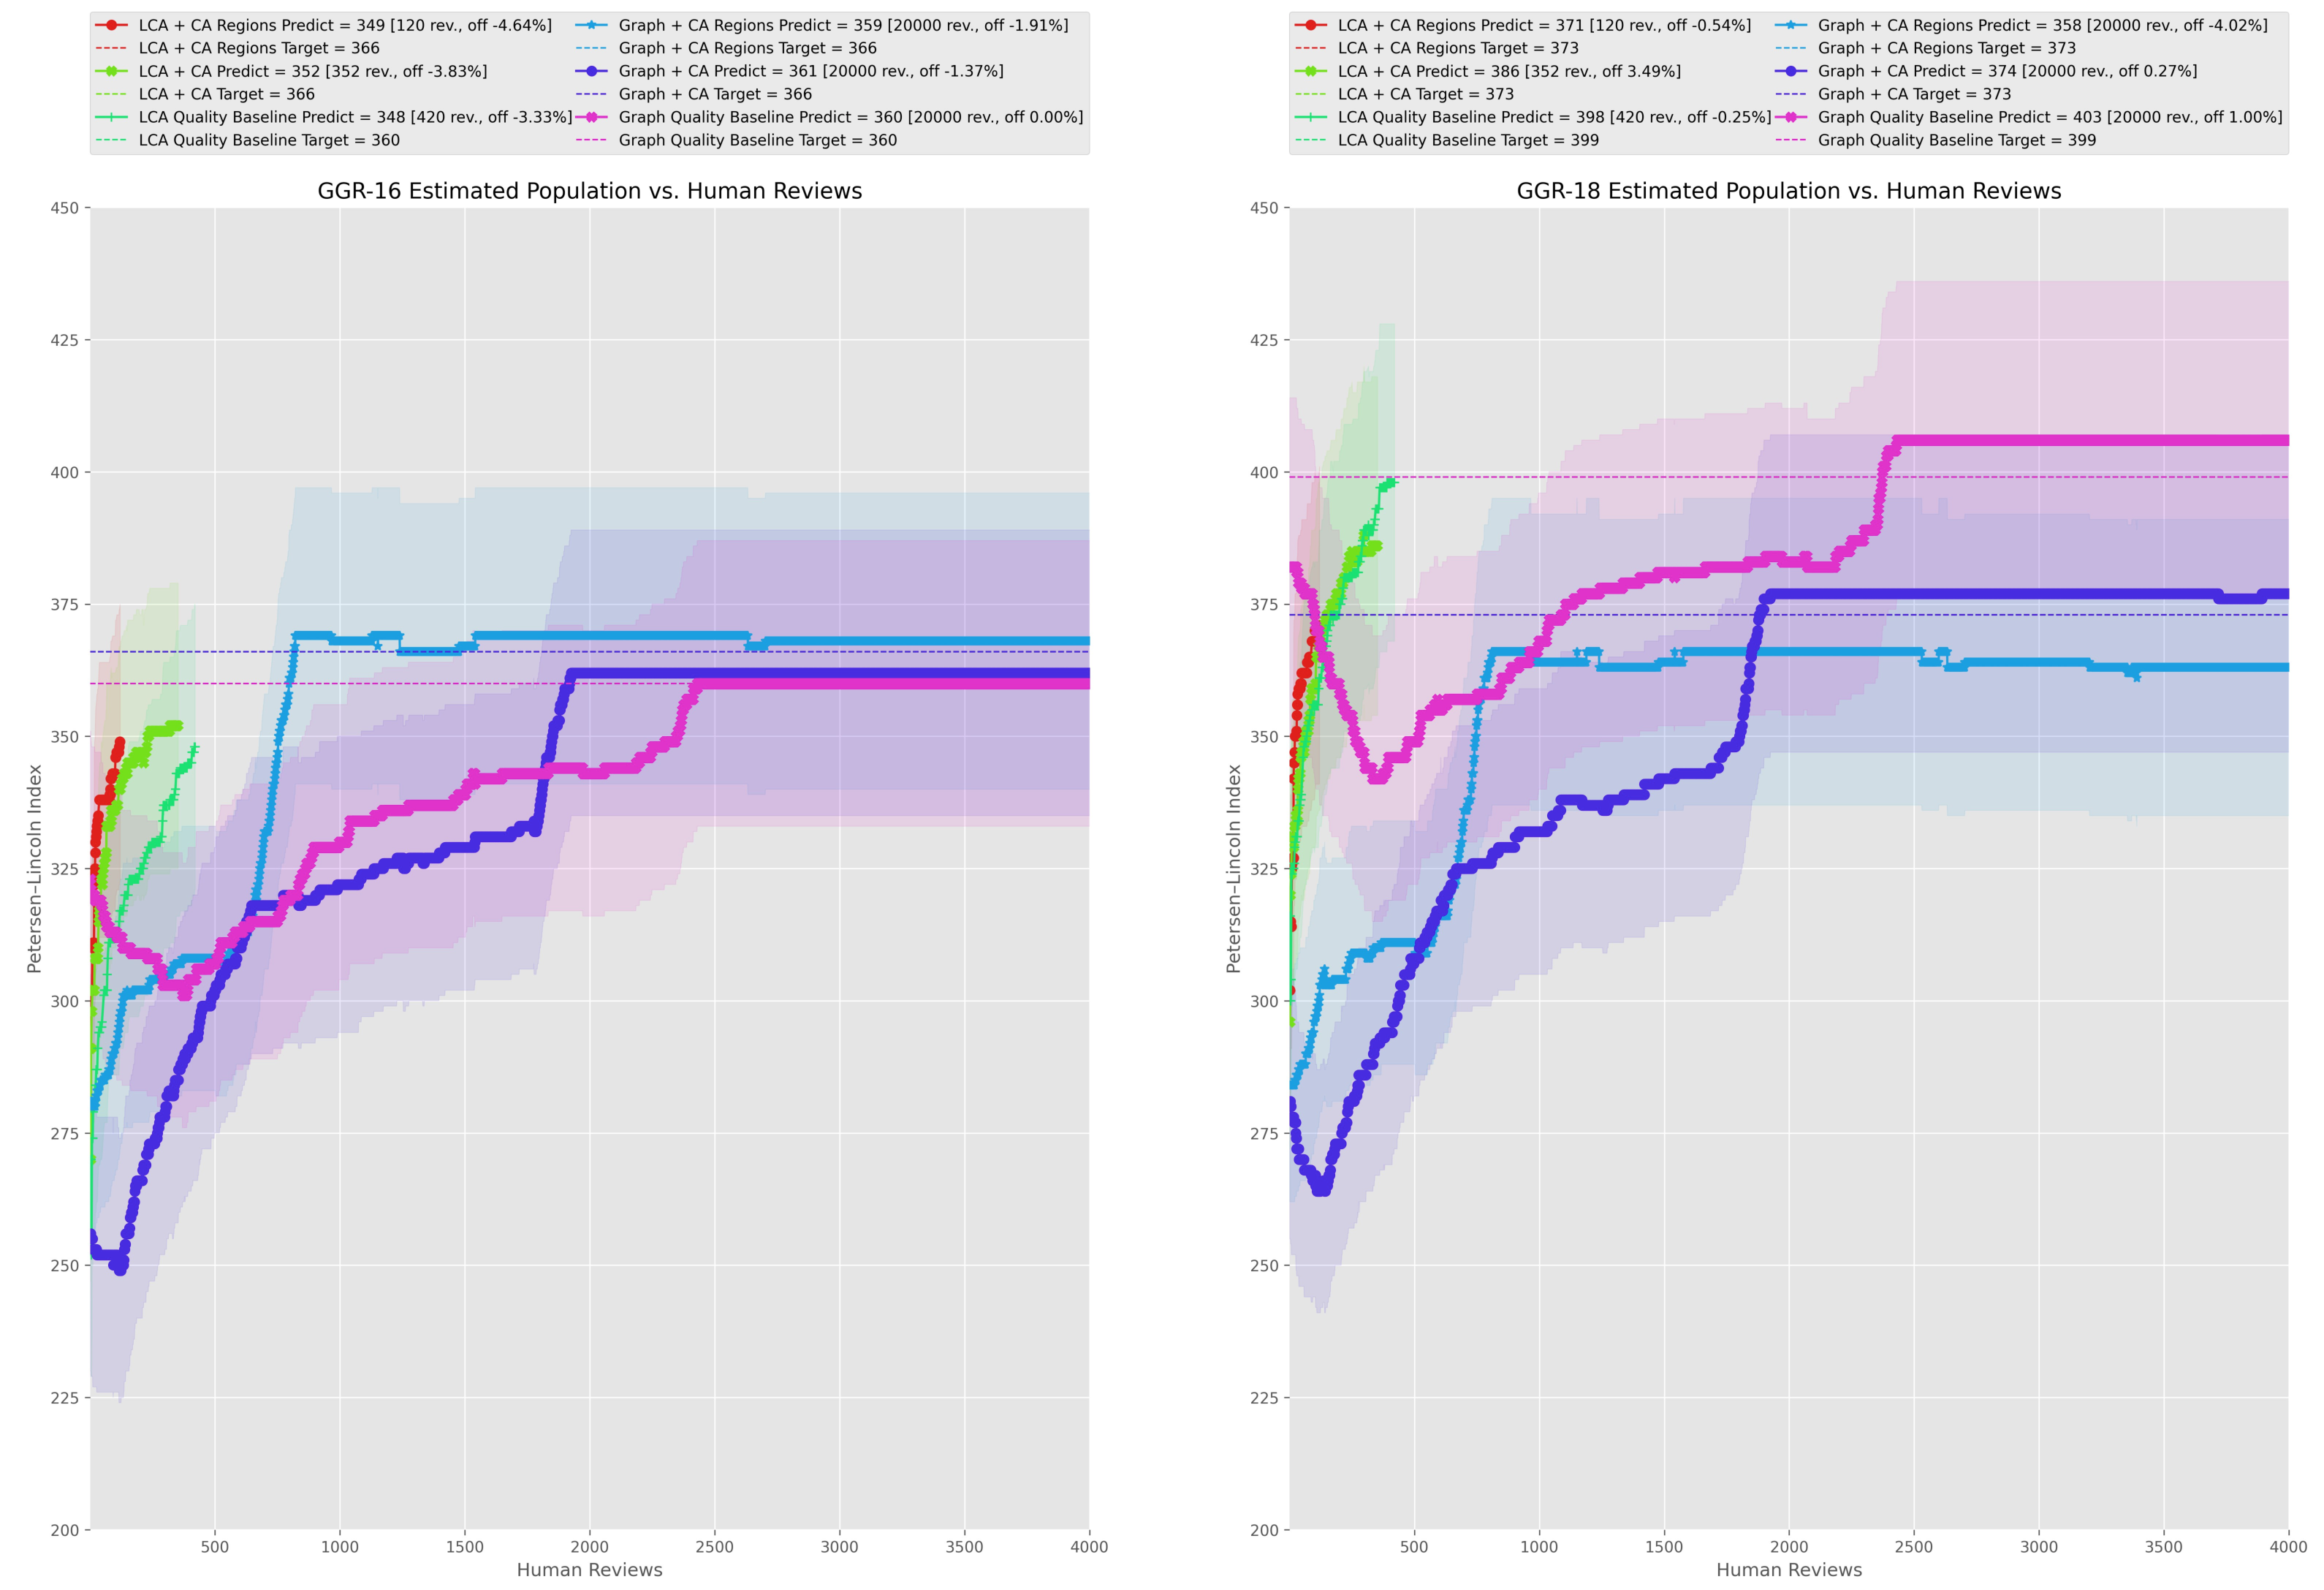
\includegraphics[width=0.9\linewidth]{resources/lca-decisions3.pdf}
    \end{center}
    \caption{The simulated population estimates over 4,000 human decisions.  Simulated Lincoln-Petersen population estimates are shown on the y-axis against the number of human decisions were requested on the x-axis.  The estimates for GGR-16 (left) and GGR-18 (right) are shown for three sets and with two separate graph curation algorithms.}
    \label{fig:ca-sim3}
\end{figure}

When a human decision was needed during the simulation, the decision was obtained by querying a \textit{perfect human oracle} (i.e., 100\% accuracy) that inferred the correct answer from the ground-truth IDs.  The oracle made perfect decisions because the goal here is to compare methods of annotation selection without needing to worry about randomness introduced by a fallible human reviewer; later experiments will examine the impact of human error in the ID curation process.  Both decision management algorithms started with fresh initialization states and were not given information about previous pair decisions used to create the ID dataset.  Each algorithm, however, was free to request as many automated and human pair decisions as it wanted during its ID curation.  Each time a human decision was requested, the current state of the algorithm's population estimate was recorded.  A log included the current number of IDs in the simulation's database, what the GGR-16 and GGR-18 population estimates were at that moment, and the number of total automated reviews requested since the start of that simulation run.  Figure~\ref{fig:ca-sim3} shows the GGR-16 (left) and GGR-18 (right) population estimates for the GZCD as a function of human decisions.  Note that a fluctuating and an indeterminate number of automated reviews may have been requested between subsequent human reviews, which is not plotted.

The format of the plot in Figure~\ref{fig:ca-sim3} is something this discussion will rely on extensively, so it is essential to understand what is being displayed and compared.  Fundamentally, the figure shows the population estimate (y-axis) as calculated in real-time after every human decision (x-axis) that was requested by a given curation configuration.  The pink dashed lines on both plots represent the ``Quality Baseline'' annotation set and its associated population estimate.  The dashed blue lines represent the population estimates calculated using the CA and CA-R annotation sets.  Thus, the dashed lines represent the target that each simulation is trying to approximate.  For example, the GGR-18 simulations on CA annotations should ideally produce 373 individuals, as indicated by the dark blue dashed line.

Something we must consider is how consistent the ground-truth population estimates are for a given input.  The GGR-16 Lincoln-Petersen index using any of the three annotation sets is approximately 360 or 366, a spread of less than 2\%.  The GGR-18 estimates are farther apart but are still relatively close (off by 26).  The ground-truth estimates with the CA and CA-R annotations are 373 IDs, while the ``Quality Baseline'' estimated 399 animal IDs (7\% spread).  While the population's actual number is unknown for both years, the GZCD has 350 ground-truth IDs for 2016.  If we were to consider the actual value of 366 (i.e., halfway between the two estimates), it implies that approximately 96\% of the surveyed animal population was seen.  A high percentage of ID coverage indicates that the photographers thoroughly saturated the survey area and produced a highly representative sampling of its population.  The effect is that the confidence intervals (95\%) for the ground-truth population estimates are relatively compact (less than $\pm$30 IDs).  Likewise, the ID database has 367 ground-truth IDs for 2018; if the actual size of IDs was 386, then the photographers sampled around 95\% of the population.  Furthermore, these coverage percentages are very high, and the number of resightings between day 1 and day 2 is also very high (approximately 220 for GGR-16 and 195 for GGR-18).  The takeaway is that while the actual number of animals is unknown, all simulations' confidence intervals overlap in their respective target population estimates and confidence intervals.

Focusing on the Graph ID performance curves for GGR-16 and GGR-18, we can see the excellent filtering effect of CA (dark blue line) vs.\ the ``Quality Baseline'' (magenta).  For the GGR-16 results, the baseline algorithm asymptotically approaches the correct number at around 2,500 human reviews, while the CA curve shows a 20\% savings in the number of human reviews.  The quality baseline estimate is precisely correct and predicts 360 individuals, while the CA prediction of 361 under-estimates its target of 366 by 1.4\%.  Likewise, the GGR-18 results show a similar savings of roughly 20\%, but the accuracy improves slightly (1\% error with quality to 0.3\% error for CA) when comparing against their respective targets.  This result indicates that using Census Annotation alone as a high-level classifier can speed up the convergence of the Graph ID algorithm while not sacrificing any meaningful accuracy in the estimate.  Comparing these results to using the Graph ID algorithm (and corresponding VAMP model) on Census Annotation Regions shows an even more drastic reduction in the number of human reviews.  The algorithm converges at around 700 human decisions (a reduction of over 70\% compared to the Quality baseline) and ends up being incorrect in its estimate by only 1.9\%.  The story for GGR-18 is similar as it also concludes at roughly the same number of reviews but does under-estimate the number of animals by 4.0\% (15 names).  It is reasonable to expect that being off by less than 5\% is acceptable for this application, especially since any bias from machine learning algorithms has not been accounted for yet.  It would seem that 5\% is well within the margin of error since the confidence interval is larger at around 7\%.  The Graph ID algorithm better approximates the ground-truth estimate (1\% error) for GGR-18 when it uses the quality baseline.

\begin{figure}[!t]
    \begin{center}
        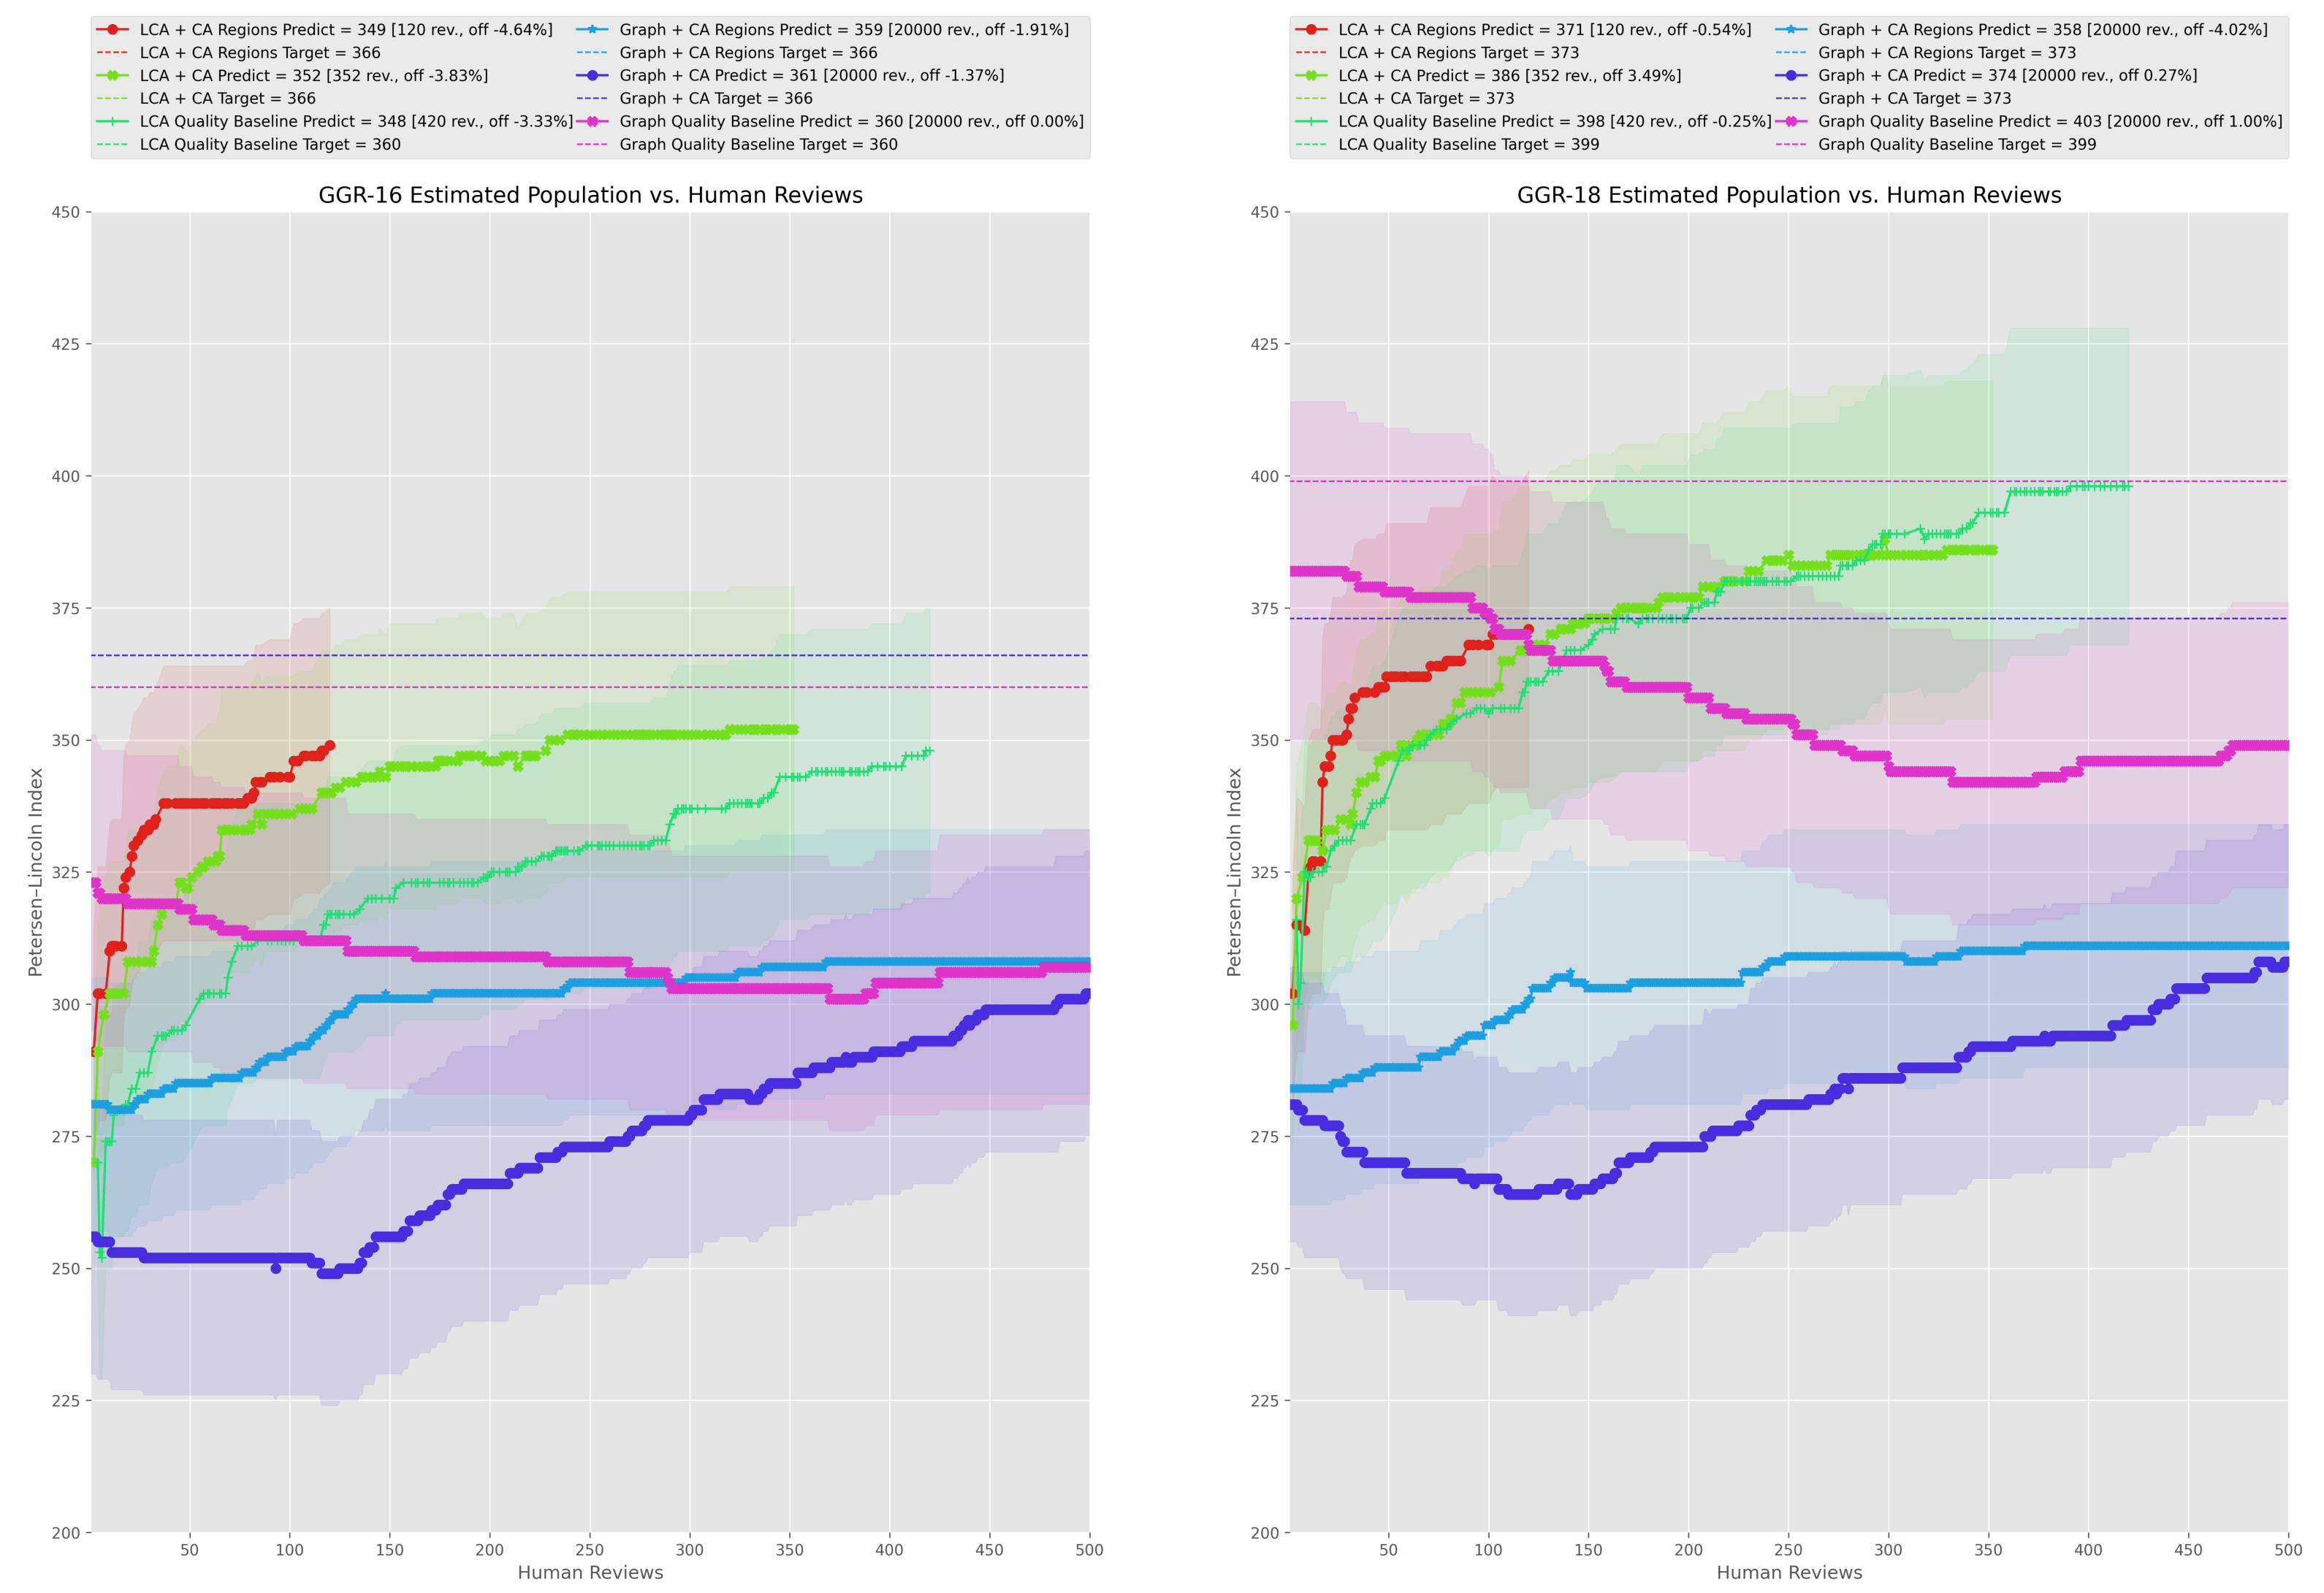
\includegraphics[width=0.9\linewidth]{resources/lca-decisions4.pdf}
    \end{center}
    \caption{The simulated population estimates over 500 human decisions.  Simulated Lincoln-Petersen population estimates are shown on the y-axis against the number of human decisions were requested on the x-axis.  The estimates for GGR-16 (left) and GGR-18 (right) are shown for three sets and with two separate graph curation algorithms.}
    \label{fig:ca-sim4}
\end{figure}

Next is a review of the LCA algorithm simulation results.  By design, LCA is focused on delaying human decision-making as much as possible. As a result, it can accurately approximate the population estimate with significantly fewer reviews than Graph ID but requires more up-front processing.  This trend is visible in Figure~\ref{fig:ca-sim3}, as the green and red LCA lines end (where the algorithm converged) at a much lower value on the x-axis compared to the blue and magenta Graph ID lines.  To better continue the analysis on LCA, a re-scaled copy of Figure~\ref{fig:ca-sim3} is provided in Figure~\ref{fig:ca-sim4}.  This second plot shows the same data but has an x-axis covering the range [1, 500] human reviews, which better displays the differences between the three LCA simulations.  The LCA algorithm on the Quality Baseline set (green line), as expected, took the most number of human reviews (420) to converge.  Because LCA does not explicitly require consistency and makes better use of the automated verifier, it can finish with much less human involvement than the Graph ID algorithm.  However, the LCA algorithm does under-estimate the target value by 3.3\% (12 names) for GGR-16.  Switching to using LCA on Census Annotations gives a final estimate within 3.8\% of the ground-truth value but saves 68 human reviews (16\% reduction).  The Census Annotation estimate also under-shoots the correct value by approximately 3.5\%, consistent with the baseline error.  This result means that using Census Annotations as a classifier only decreases the relative accuracy by 0.5\%.  Just as with the Graph ID algorithm, the LCA algorithm drastically improves automation when Census Annotation Regions are used.  The number of required human reviews for the most automated decision management algorithm configuration was only 120 in total and is accurate within 4.6\% on GGR-16 data (predicting 349 animals against a ground-truth value of 366).  The results for GGR-18 mirror the narrative from the GGR-16 results, with LCA run on Census Annotation Regions predicting the correct answer within 0.5\% (under-shooting by two names).  The Quality Baseline LCA results were off by only one name but ended up needing nearly four times the number of human reviews.

\subsubsection{Census Annotation Decision Thresholds}

\begin{figure}[!t]
    \begin{center}
        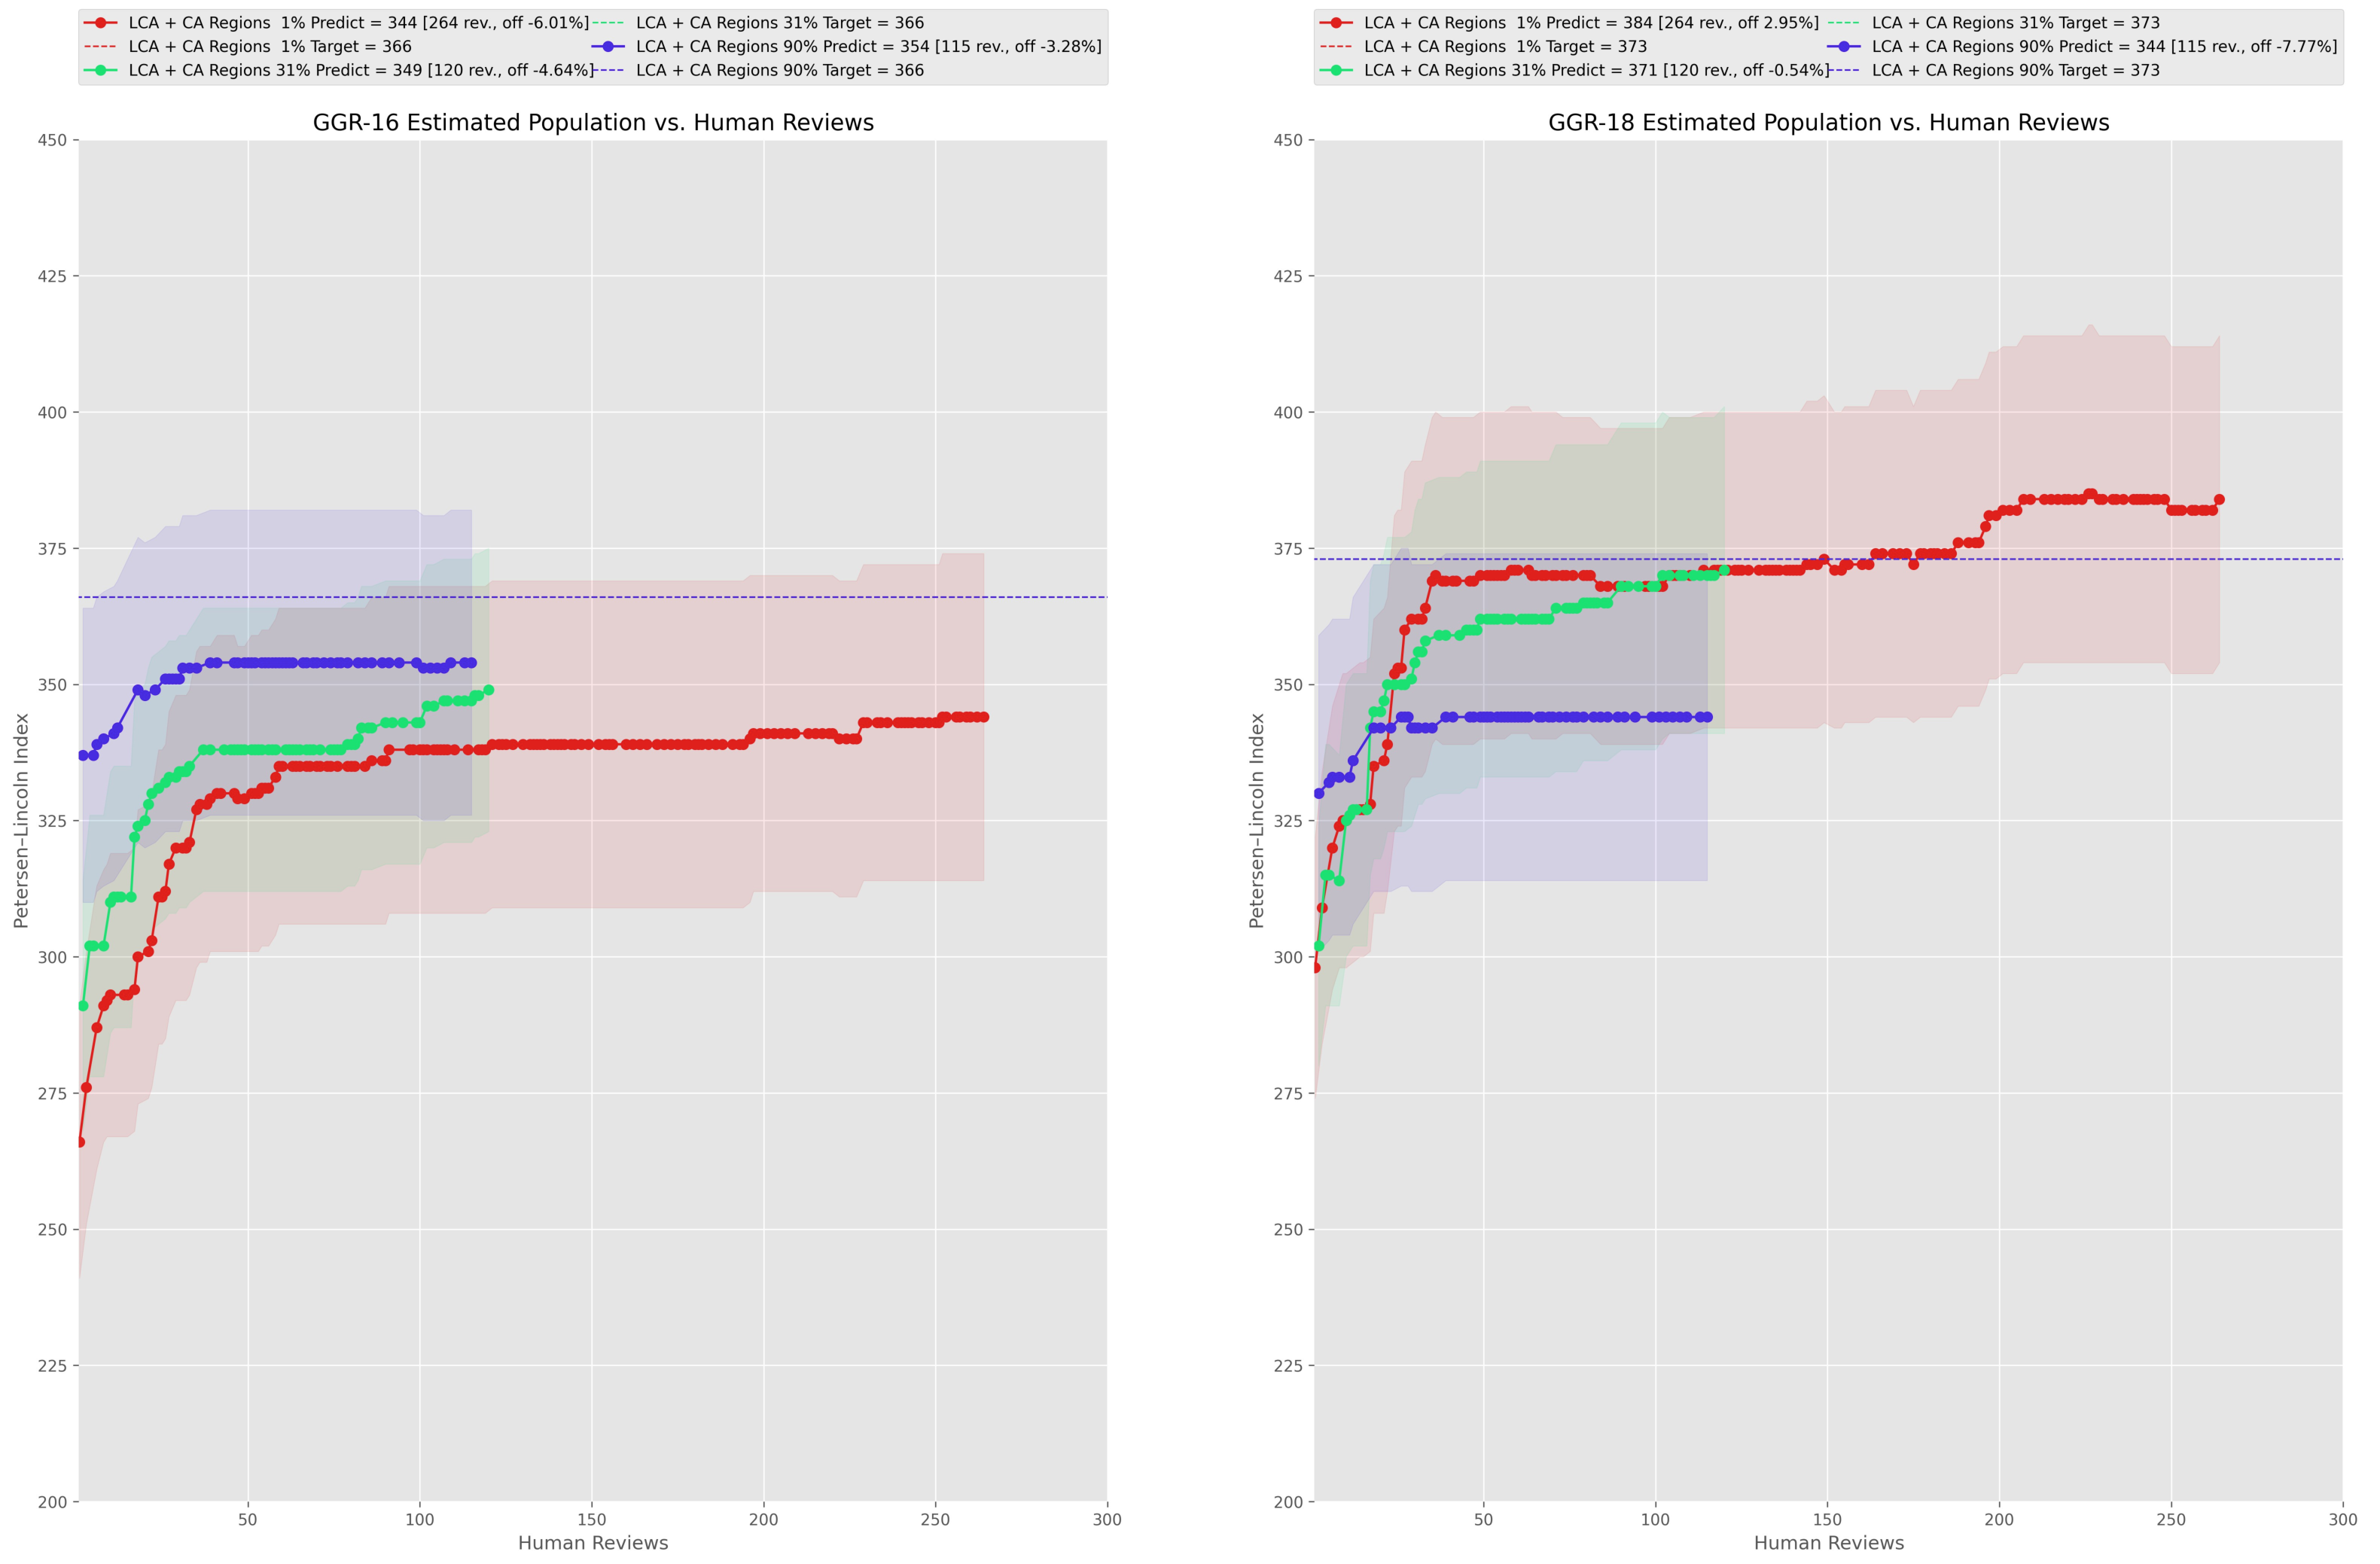
\includegraphics[width=0.9\linewidth]{resources/lca-decisions-harsh-lax-1.pdf}
    \end{center}
    \caption{The simulated population estimates across different Census Annotation thresholds.  Simulated Lincoln-Petersen population estimates are shown on the y-axis against the number of human decisions were requested on the x-axis.  The estimates for GGR-16 (left) and GGR-18 (right) are shown for three different sets of Census Annotation Regions, selected with thresholds at 1\%, 31\% (recommended), and 90\%.}
    \label{fig:ca-sim-harsh-lax}
\end{figure}

We also can quickly consider what would happen when the Census Annotation thresholds are changed from the recommended 31\% to lower and higher values.  If the filtering threshold is lowered to 1\%, the number of used annotations will increase but for the added risk of incomparable and incidental matches.  As we have established, these errors will result in more overall work and likely bias the estimate higher.  On the other hand, a high filtering threshold of 90\% will provide very clean and comparable animal sightings to animal ID curation, making it much more likely to miss a relevant animal sighting.  Figure~\ref{fig:ca-sim-harsh-lax} shows the simulations for these two cases with the LCA algorithm and CA-Rs as the input data.  We can see that the 1\% population estimates for GGR-16 and GGR-18 (red line) require much more work to converge, and the algorithm achieves a worse result.  Likewise, using a very high CA filtering threshold of 90\% (blue line) does not increase work compared to the recommended 31\% (green line) and under-shoots the target by 7.8\% for GGR-18.  That being said, the simulated value is still within the confidence interval for those two populations.

In summary, Census Annotation -- and more specifically Census Annotation Regions -- is a powerful tool for increasing automation through effective filtering.  Furthermore, this improvement can be seen with two entirely different decision management algorithms.  For example, comparing LCA on Census Annotation Regions to Graph ID on the ``Quality Baseline'', the latter required over 2,500 reviews to closely approximate the target estimate (and over 10,000 reviews to get within 1\% on GGR-18).  In contrast, LCA with CA-R required only 120 human decisions to get within 5\% of the ground-truth estimate on GGR-16 and 0.5\% for GGR-18.  We can also see that photographic censusing is somewhat sensitive to how well Census Annotations are filtered. Therefore, we want to remove annotations that cause errors and include as many annotations as possible for accurate estimates.  When the CA filtering was at 90\%, the estimate decreased.  This decrease seems to defy the conclusions of Equation~\eqref{eq:final}; the problem is that the threshold is putting pressure on Assumptions 3 and 4 (see Section~\ref{sec:assumptions}), and the estimate is therefore not reliable.  Next, we compare how much of the overall ID curation work each decision management algorithm is automating with algorithmic verifiers.

\subsection{Degree of Decision Automation}

During each of the six simulations from the previous sub-section, the total number of requested VAMP decisions were recorded after each human decision.  Each simulation used HotSpotter as the ranker and VAMP as the verifier but varied on their input annotation sets and the decision management algorithm used.  We can contrast the total number of automated verification decisions requested to cross-examine how much of the overall ID curation process was automated.  For example, it was shown earlier in this chapter that VAMP automates a higher percentage of decisions (for a fixed FPR) when Census Annotation and Census Annotation Regions are used.  Allowing VAMP to perform more of the overall ID curation work implies that the process also requires less work from a human reviewer.

\begin{table}[!t]
    \caption{The amount of work done by the automated verifier reduces the number of human reviews. For the Graph ID algorithm, a simulation was considered \textit{converged} when the number of requested human reviews exceeded 20,000.  The average number of VAMP reviews per annotation in parenthesis is below the number of VAMP Reviews.  We can see that using LCA on CA Regions results in the lowest number of human decisions.}
    \label{table:vamp-work}
    \begin{center}
        \begin{tabular}{| l | l | r | r | r | r | r |}
            \hline
            \textbf{Algorithm}    & \textbf{Set} & \textbf{Annotations} & \textbf{VAMP}    & \textbf{Human}   & \textbf{Total}   & \textbf{Automation} \\
                                  &              &                      & \textbf{Reviews} & \textbf{Reviews} & \textbf{Reviews} & \textbf{Rate}       \\
            \hline
            \hline
            Graph ID              & Quality      & 4,269                & 20,374           & 20,000           & 40,374           & 50.5\%              \\
            \textit{Converged}    & Baseline     &                      & (4.8)            &                  &                  &                     \\
            \hline
            Graph ID              & CA           & 4,142                & 19,055           & 20,000           & 39,055           & 48.8\%              \\
            \textit{Converged}    &              &                      & (4.6)            &                  &                  &                     \\
            \hline
            Graph ID              & CA           & 4,142                & 22,088           & 20,000           & 42,088           & 52.5\%              \\
            \textit{Converged}    & Region       &                      & (5.3)            &                  &                  &                     \\
            \hline
            \hline
            Graph ID              & Quality      & 4,269                & 12,988           & 2,414            & 15,402           & 84.3\%              \\
            \textit{Approximated} & Baseline     &                      & (3.0)            &                  &                  &                     \\
            \hline
            Graph ID              & CA           & 4,142                & 13,187           & 1,923            & 15,110           & 87.3\%              \\
            \textit{Approximated} &              &                      & (3.2)            &                  &                  &                     \\
            \hline
            Graph ID              & CA           & 4,142                & 4,911            & 642              & 5,553            & 88.4\%              \\
            \textit{Approximated} & Region       &                      & (1.2)            &                  &                  &                     \\
            \hline
            \hline
            Graph ID              & Quality      & 4,269                & 5,000            & 2,255            & 7,255            & 68.9\%              \\
            \textit{Budgeted}     & Baseline     &                      & (1.2)            &                  &                  &                     \\
            \hline
            Graph ID              & CA           & 4,142                & 5,000            & 1,747            & 6,747            & 74.1\%              \\
            \textit{Budgeted}     &              &                      & (1.2)            &                  &                  &                     \\
            \hline
            Graph ID              & CA           & 4,142                & 5,000            & 645              & 5,645            & 88.6\%              \\
            \textit{Budgeted}     & Region       &                      & (1.2)            &                  &                  &                     \\
            \hline
            \hline
            LCA                   & Quality      & 4,269                & 22,552           & 420              & 22,972           & 98.2\%              \\
            \textit{Converged}    & Baseline     &                      & (5.3)            &                  &                  &                     \\
            \hline
            LCA                   & CA           & 4,142                & 18,255           & 352              & 18,607           & 98.1\%              \\
            \textit{Converged}    &              &                      & (4.4)            &                  &                  &                     \\
            \hline
            LCA                   & CA           & 4,142                & 13,307           & 120              & 13,427           & 99.1\%              \\
            \textit{Converged}    & Region       &                      & (3.2)            &                  &                  &                     \\
            \hline
            \hline
            LCA                   & Quality      & 4,269                & 5,000            & 121              & 5,121            & 97.6\%              \\
            \textit{Budgeted}     & Baseline     &                      & (1.2)            &                  &                  &                     \\
            \hline
            LCA                   & CA           & 4,142                & 5,000            & 92               & 5,092            & 98.2\%              \\
            \textit{Budgeted}     &              &                      & (1.2)            &                  &                  &                     \\
            \hline
            LCA                   & CA           & 4,142                & 5,000            & 63               & 5,063            & 98.8\%              \\
            \textit{Budgeted}     & Region       &                      & (1.2)            &                  &                  &                     \\
            \hline
        \end{tabular}
    \end{center}
\end{table}

For the Graph ID simulations, the algorithm either converged or was prematurely stopped after 20,000 human decisions.  Even though the algorithm had not officially converged, that does not mean it was not closely approximating the target estimate well before its termination.  For each Graph ID simulation, there is a distinct point where the algorithm approximately converges, and it is helpful to track this point for comparison.  For the Quality Baseline set, this point is at 2,414 human reviews; for the CA set, it is at 1,923 reviews; and for the CA Regions, it is at 642 reviews.  If the Graph ID algorithm were stopped prematurely at each of these junctures, the predicted estimates would have all been within 5\% correct.  Another way to consider the work done by an automated verifier is to cap its total number of decisions.  For example, pretend that the automated verifier was very slow, much slower than a human, or was computationally expensive.  In that case, we may want to consider placing a budget on the total number of automated decisions before terminating. For example, a fixed budget of 5,000 automated reviews would mean that each annotation in the three evaluation sets participates in at least two reviews on average.  Table~\ref{table:vamp-work} provides a breakdown for the number of human and VAMP decisions that were needed for each annotation set and decision management algorithm.  For the Graph ID algorithm, the table offers the termination points at 20,000 decisions, points where the correct value is approximated, and early-stopping points based on a strictly enforced budget.

The results show that using Census Annotation Regions improves the rate of automation compared to the Quality Baseline. For example, the Graph ID algorithm converged (terminated at 20,000 human reviews) with 50.5\% of the total reviews being automatically decided by VAMP.  In contrast, Graph ID on CA Regions automated a total of 52.5\% of the reviews, a savings of 1,714 reviews. In addition, VAMP is doing more work overall on Census Annotation Regions as there are 5.3 decisions per annotation on average compared to 4.8 for the Quality Baseline.  For the Quality Baseline, the VAMP model was able to automate 12,988 reviews, with an automation rate of 84.2\%  The Census Annotation, while requiring approximately the same number of overall reviews as the baseline set (15,402 vs.\ 15,110, a difference of less than 2\%), required significantly fewer human reviews at 1,923 and an automation rate of 87.3\%. Thus, using Census Annotations saved the human reviewers from needing to complete nearly 500 reviews, a 20.3\% reduction.  Going a step further, Census Annotation Regions require only 5,553 total reviews to approximate the estimate, with only 642 being done by a human.  Compared to using Graph ID on the Quality Baseline set, using CA Region with the same algorithm results in a 73.4\% reduction in human work.

Furthermore, the LCA algorithm with the Quality Baseline set is highly automated.  In total, it makes 22,972 decisions and asks for only 420 of those from a human (automation rate of 98.2\%).  The LCA algorithm is designed to try alternative clustering of the current ID graph, which calls for an automated or human decision.  The algorithm's degree of confidence in a particular clustering can be partially seen in how many reviews are requested before the algorithm converges.  This behavior means that the algorithm will converge faster if the decisions are coherent, the annotations are discriminative, and the edge weights are stable. For example, the LCA algorithm converges faster with Census Annotations with a total number of reviews of 18,607 (automation rate of 98.1\%); the algorithm can converge with 4.4 decisions per annotation compared to 5.3 with the quality baseline, indicating that the former was more discriminate and required fewer alternative clusterings.  The CA Regions shows a dramatic reduction in the number of total reviews at 13,427 while only requiring 120 from a human (99.1\% automated).  This result represents a 71.4\% reduction in human work and an even lighter workload at 3.2 decisions per annotation.

Considering a budget restriction with the Quality Baseline set, the Graph ID algorithm only automated 68.9\% of the reviews. In contrast, using Census Annotation automates 74.1\%, and using Census Annotation Regions achieves a rate of 88.6\%.  A similar -- albeit less dramatic -- improvement in automation occurs using the LCA algorithm; using CA Regions and a budget cuts the number of human decisions in half (to 63) compared to the Quality Baseline of 121.  In summary, these results indicate that Census Annotation Regions improve automation for both the Graph ID and LCA decision management algorithms.  Furthermore, LCA can make much more efficient use of the automated verifier than Graph ID.


\subsection{Comparison of Automated Ranker \& Verifier}

\begin{figure}[!t]
    \begin{center}
        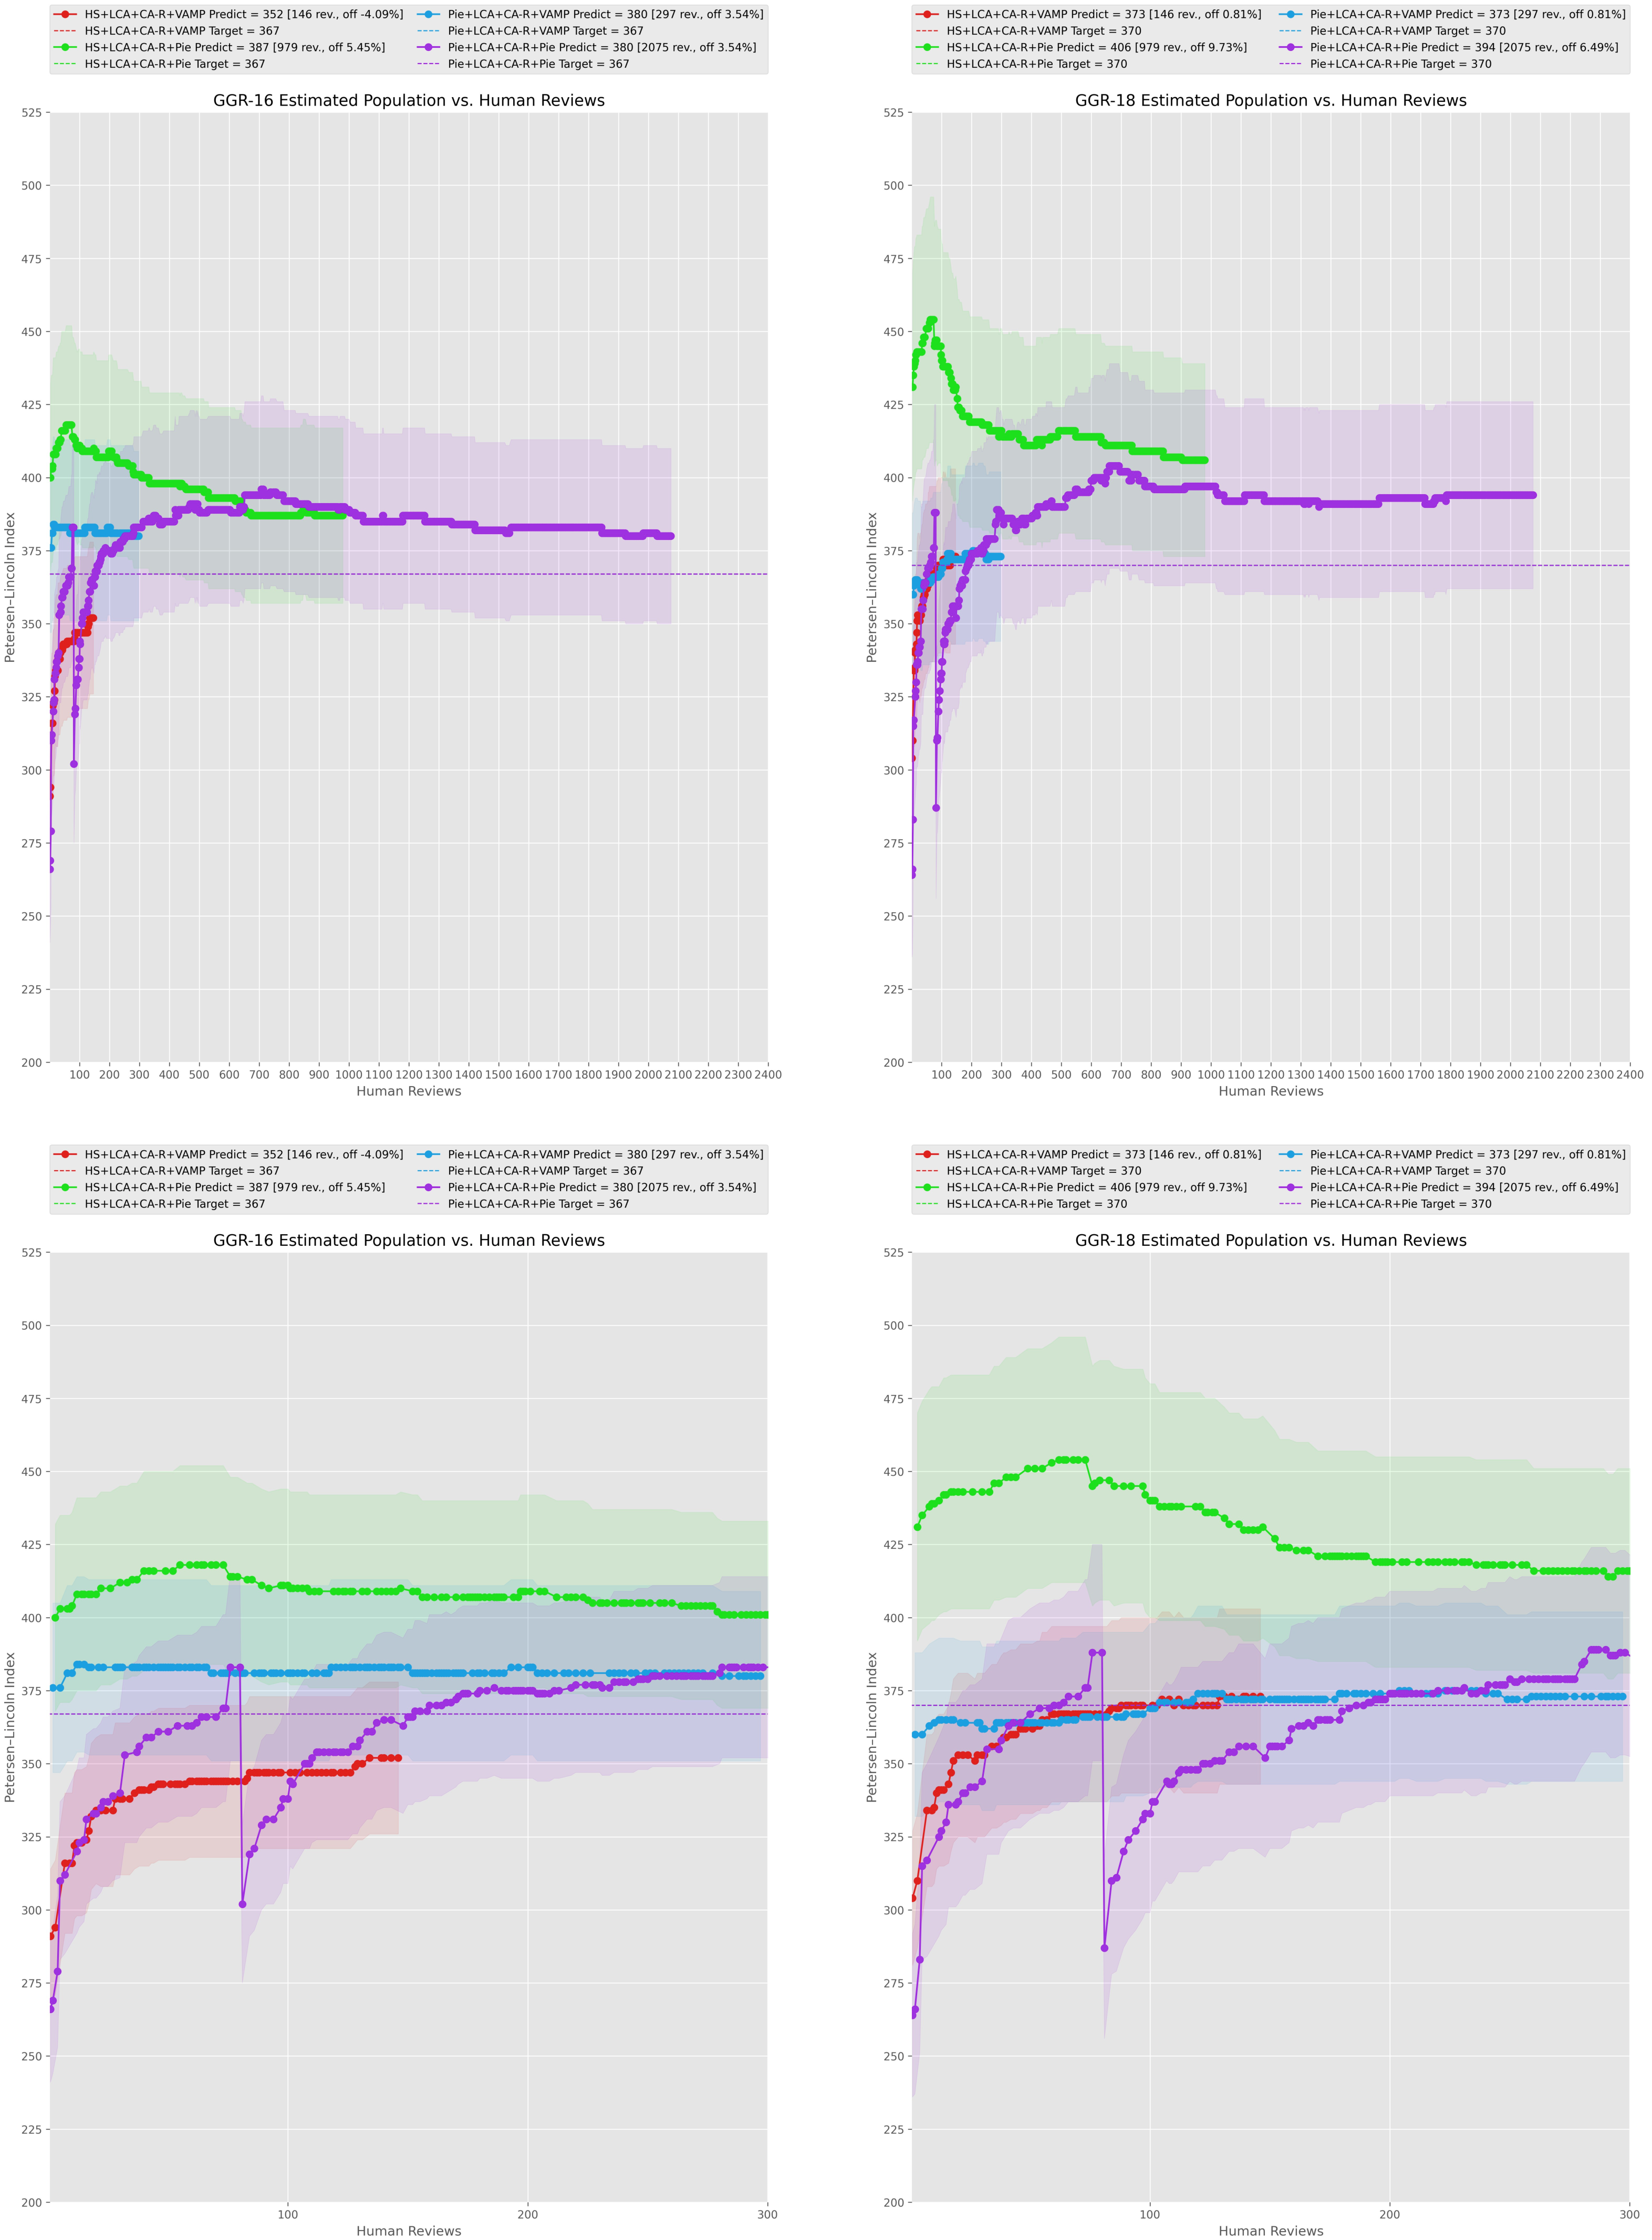
\includegraphics[width=0.82\linewidth]{resources/lca-decisions-compare-1.pdf}
    \end{center}
    \caption{The simulated population estimates with different ranking and verification algorithms.  Simulated Lincoln-Petersen population estimates are shown on the y-axis against the number of human decisions were requested on the x-axis.  The estimates for GGR-16 (left) and GGR-18 (right) are shown for different ranking and verification algorithms.}
    \label{fig:ca-sim-compare}
\end{figure}

We next consider the impact that different ranking and verification algorithms have on photographic censusing.  As discussed in Chapters~\ref{chapter:related} and~\ref{chapter:overview}, the HotSpotter algorithm was developed alongside the detection pipeline presented here, the VAMP verifier, and the Graph ID decision management algorithm for the problem of estimating Gr\'evy's zebra populations. Therefore, it is apparent and unsurprising that most of the photographic censusing analysis presented in this dissertation relies on it heavily.  This preference is due to 1) its ability to match sightings without any species-specific training, 2) it does not rely on extensive ground-truth ID data to bootstrap, and 3) it is fast to produce accurate results.  For similar reasons, the VAMP verifier is used thus far to automate human decision-making for Gr\'evy's zebra.  Even though both approaches are the presumed defaults, they are not the only options available for the automated ranking and verification tasks.  Specifically, the PIE~\cite{moskvyak_robust_2019} algorithm can be trained to perform both tasks (ranking and verification) as a triplet-loss neural network.

The PIE algorithm is helpful to photographic censusing for many reasons: 1) it has a superior feature extraction process compared to HotSpotter (which is based on the outdated SIFT algorithm), 2) it is exceedingly fast (and supports GPU acceleration during training and inference), and 3) it is highly accurate for known, consistent poses of an animal (e.g., a right-facing Census Annotation Region).  Furthermore, the PIE algorithm produces a single, fixed-length feature vector per annotation, which can be quickly computed, cached, and compared in L2 space for fast matching (e.g., clustering with approximate nearest neighbors) and verification (e.g., a distance threshold).  The downside is that PIE requires an existing ID database to train and cannot be bootstrapped without prior IDs.  After building a relatively large ID dataset like GZCD with HotSpotter, however, PIE can be trained to perform accurate matching and verification.  The model can also be used to identify ground-truth ID errors that HotSpotter was unable to recognize, improving the reliability of the ID database and providing even better data for re-training the PIE algorithm.

With CA-R for input annotations, HotSpotter for ranking, VAMP for verifying, PIE for ranking and verifying, LCA for curation, simulated humans for verifying, and Lincoln-Petersen for estimating the population, we have all of the tools at our disposal for robust photographic censusing.  Figure~\ref{fig:ca-sim-compare} shows a comparison of four simulations:

\begin{enumerate}
    \item \textbf{Red Line} - Input: CA-R, Ranker: HotSpotter, Verifier: VAMP, Curation: LCA
    \item \textbf{Green Line} - Input: CA-R, Ranker: HotSpotter, Verifier: PIE, Curation: LCA
    \item \textbf{Blue Line} - Input: CA-R, Ranker: PIE, Verifier: VAMP, Curation: LCA
    \item \textbf{Purple Line} - Input: CA-R, Ranker: PIE, Verifier: PIE, Curation: LCA
\end{enumerate}

\noindent The figure shows GGR-16 (left) and GGR-18 (right) results for two x-axis scales.  The top row shows the same result for a maximum of 2,400 human decisions, and the bottom row uses a maximum of 300 decisions.

All four simulations end with a population estimate within 5.5\% for GGR-16 and 10\% for GGR-18.  The clearest outliers are for the simulations where PIE operates as the verifier, consistently over-shooting the target.  Upon inspection, PIE is performing so poorly because it is sensitive to changes in pose and comparable quality.  The majority of the extra IDs that PIE suggests is where it takes a sizeable single ID and splits it into two IDs, with one ID containing only 1-2 annotations and the second ID containing all other annotations for that ground-truth ID.  This result suggests that PIE can be helpful to identify outlier Census Annotation Regions that are on the border of being comparable.  Furthermore, for GGR-16 and GGR-18, the PIE ranking algorithm with VAMP as the verifier was the most accurate configuration (3.5\% error and 0.8\%, respectively).  Compared to HotSpotter with VAMP, however, that best result came at the cost of double the number of human reviews.

In summary, the HotSpotter and PIE algorithms work well as ranking algorithms for Gr\'evy's zebra.  However, using PIE for animal ID curation inflates the overall estimate because pose variations are challenging for that algorithm, and careful attention should be paid to animal IDs with only a few annotations.  We will conclude this chapter by examining the impact human decision errors have on animal ID curation.

\subsection{Effect of Human Verification Accuracy}

\begin{figure}[!t]
    \begin{center}
        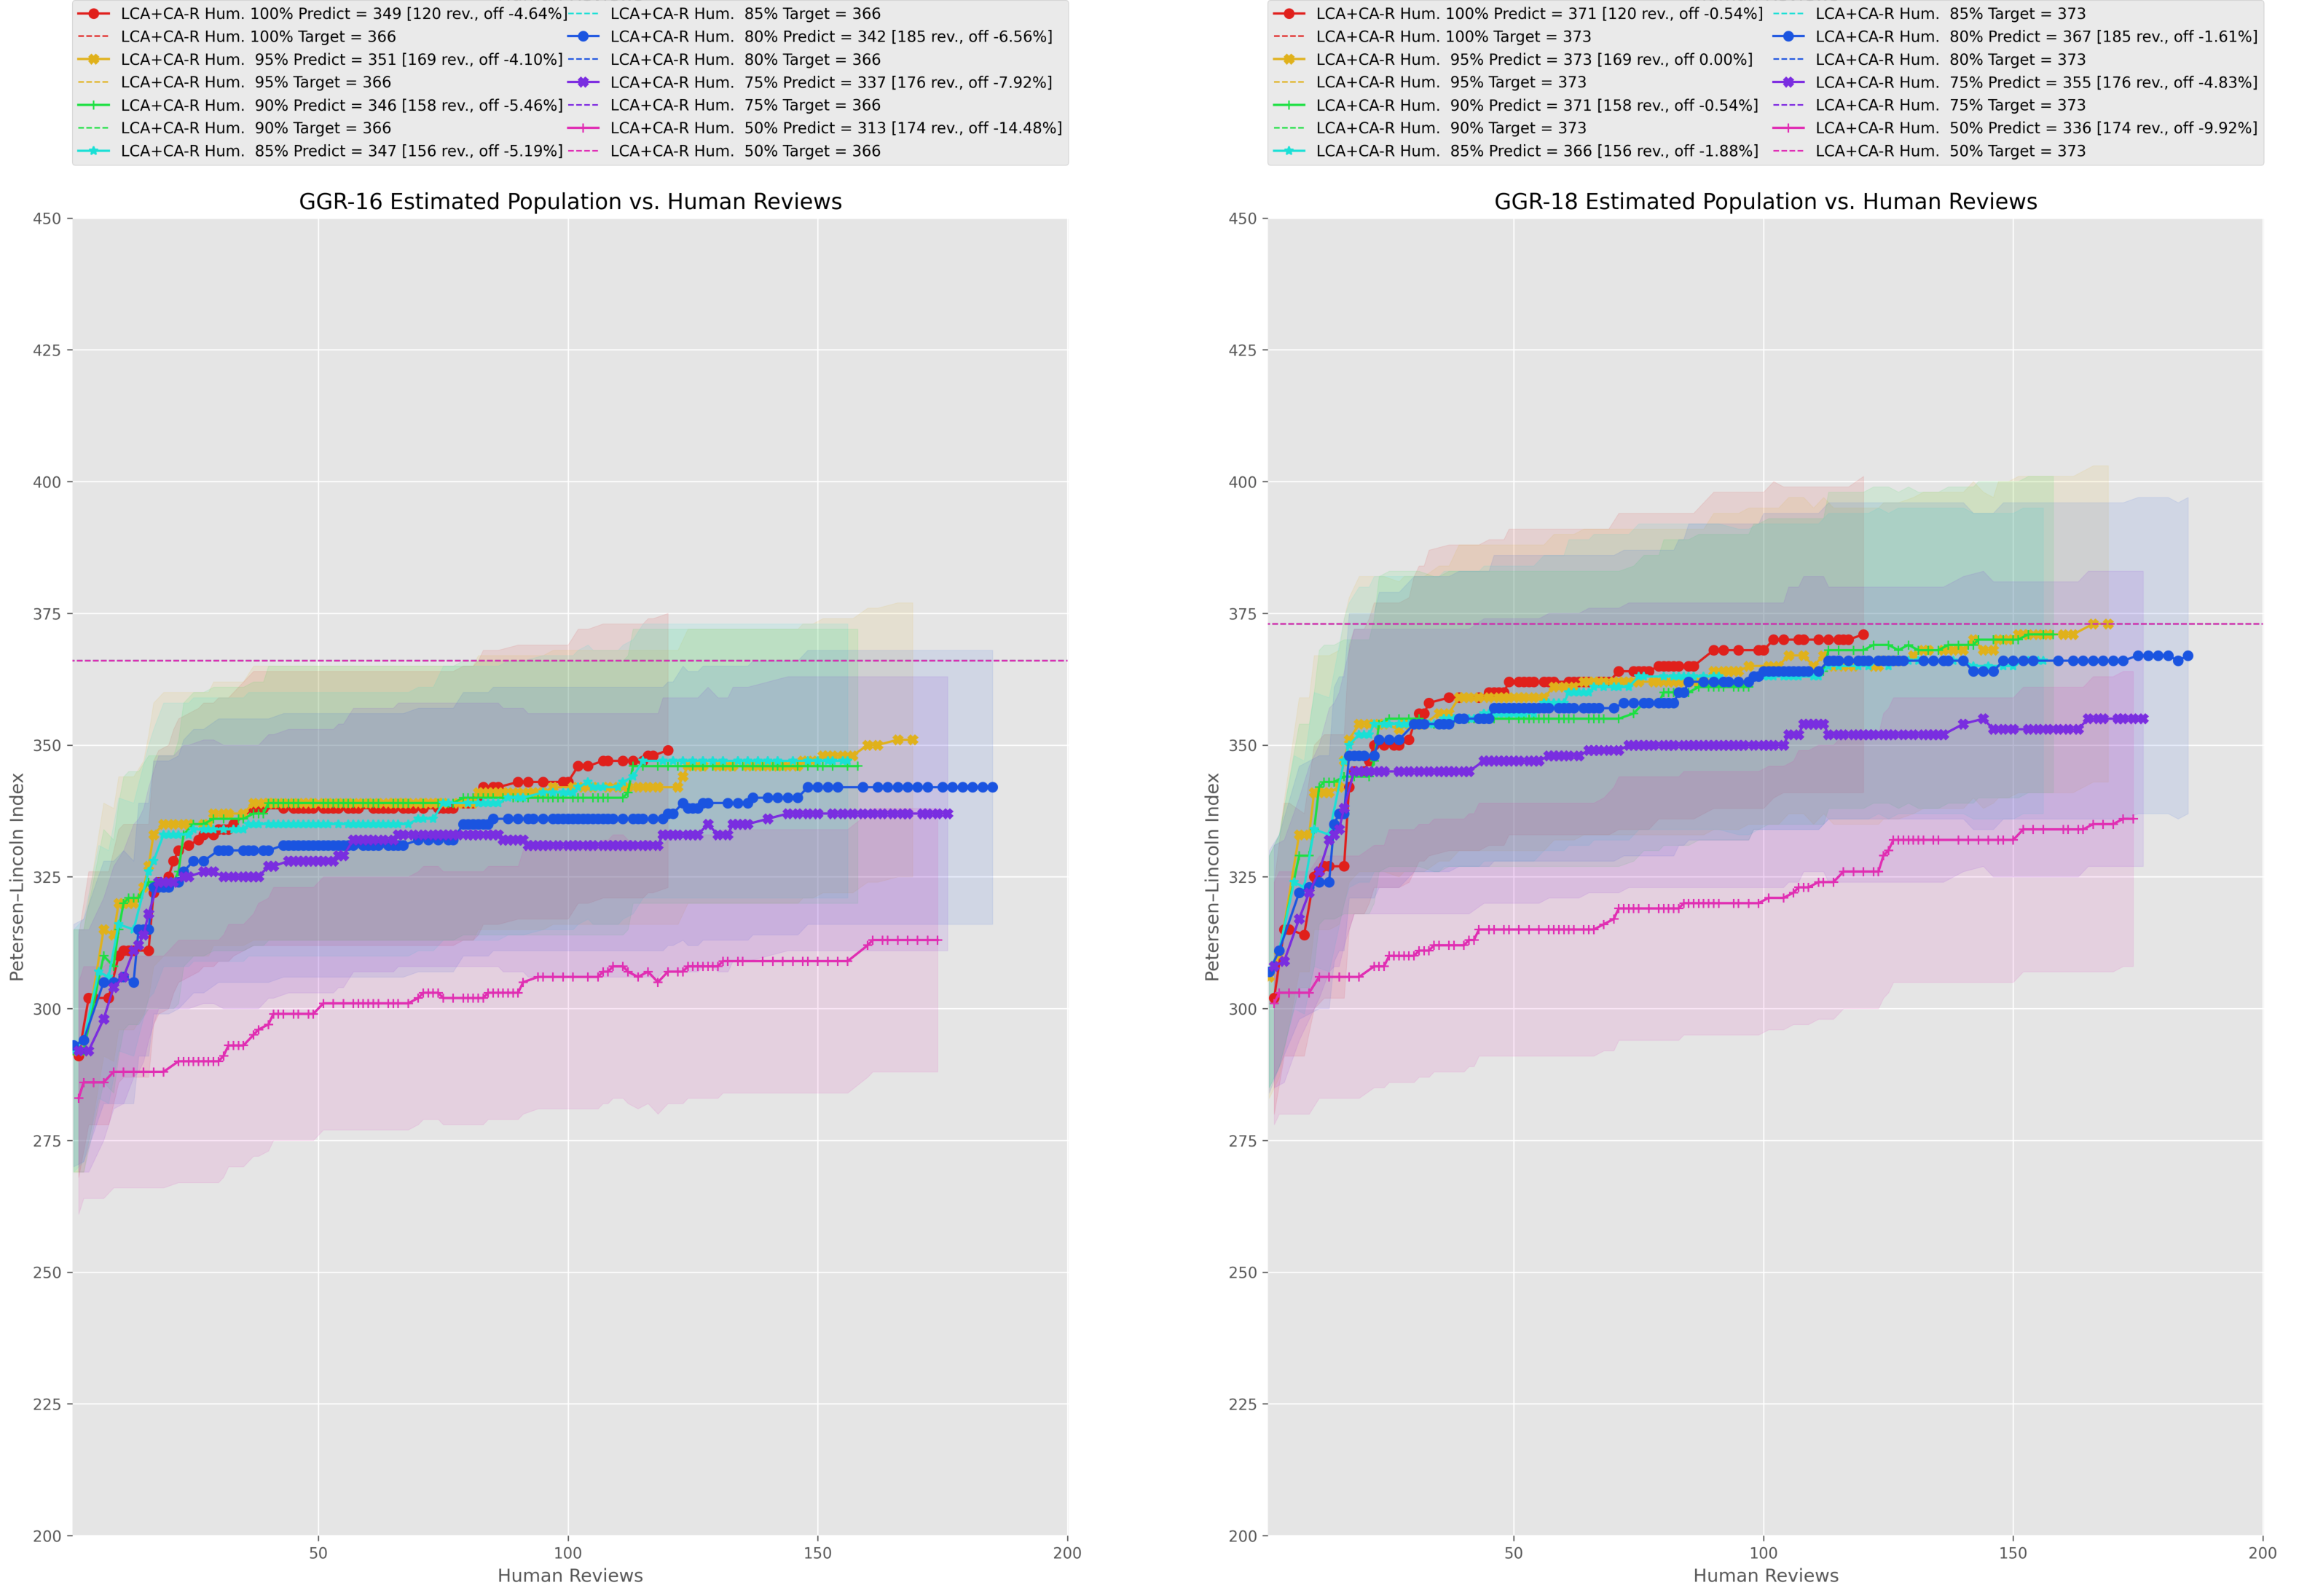
\includegraphics[width=0.9\linewidth]{resources/lca-decisions-humans-1.pdf}
    \end{center}
    \caption{The simulated population estimates across different human accuracies.  Simulated Lincoln-Petersen population estimates are shown on the y-axis against the number of human decisions were requested on the x-axis.  The estimates for GGR-16 (left) and GGR-18 (right) are shown for different simulated levels of human decision accuracy, ranging from 50\% to 100\%.}
    \label{fig:ca-sim-humans}
\end{figure}

All of the simulations above have used a perfect human oracle whenever a manual decision is needed.  This oracle was configured to have a guaranteed accuracy of 100\% so that any effects from human fallibility are removed, and the different algorithms can be compared in a more standardized environment.  The expectation that the human is always perfect is unrealistic, however, even for Census Annotation Regions.  Looking back to the user study in Section~\ref{sec:user-study}, we can recall that an expert human reviewer's accuracy is around 98\% on average for general pairs of annotations, and novice reviewers are approximately 94\% accurate.  The lowest accuracy measured for a human reviewer during that study was 91.7\%, so a minimum expectation of 90\% seems realistic as a test condition.  To compare the impact of poor human decision-making, we can simulate the human oracle with varying levels of random error for a fixed animal ID configuration.  The simulations in this sub-section were completed with CA Regions as the input annotation set, HotSpotter as the ranker, VAMP as the verifier, and LCA as the decision management algorithm to keep the comparisons simple.

\begin{figure}[!t]
    \begin{center}
        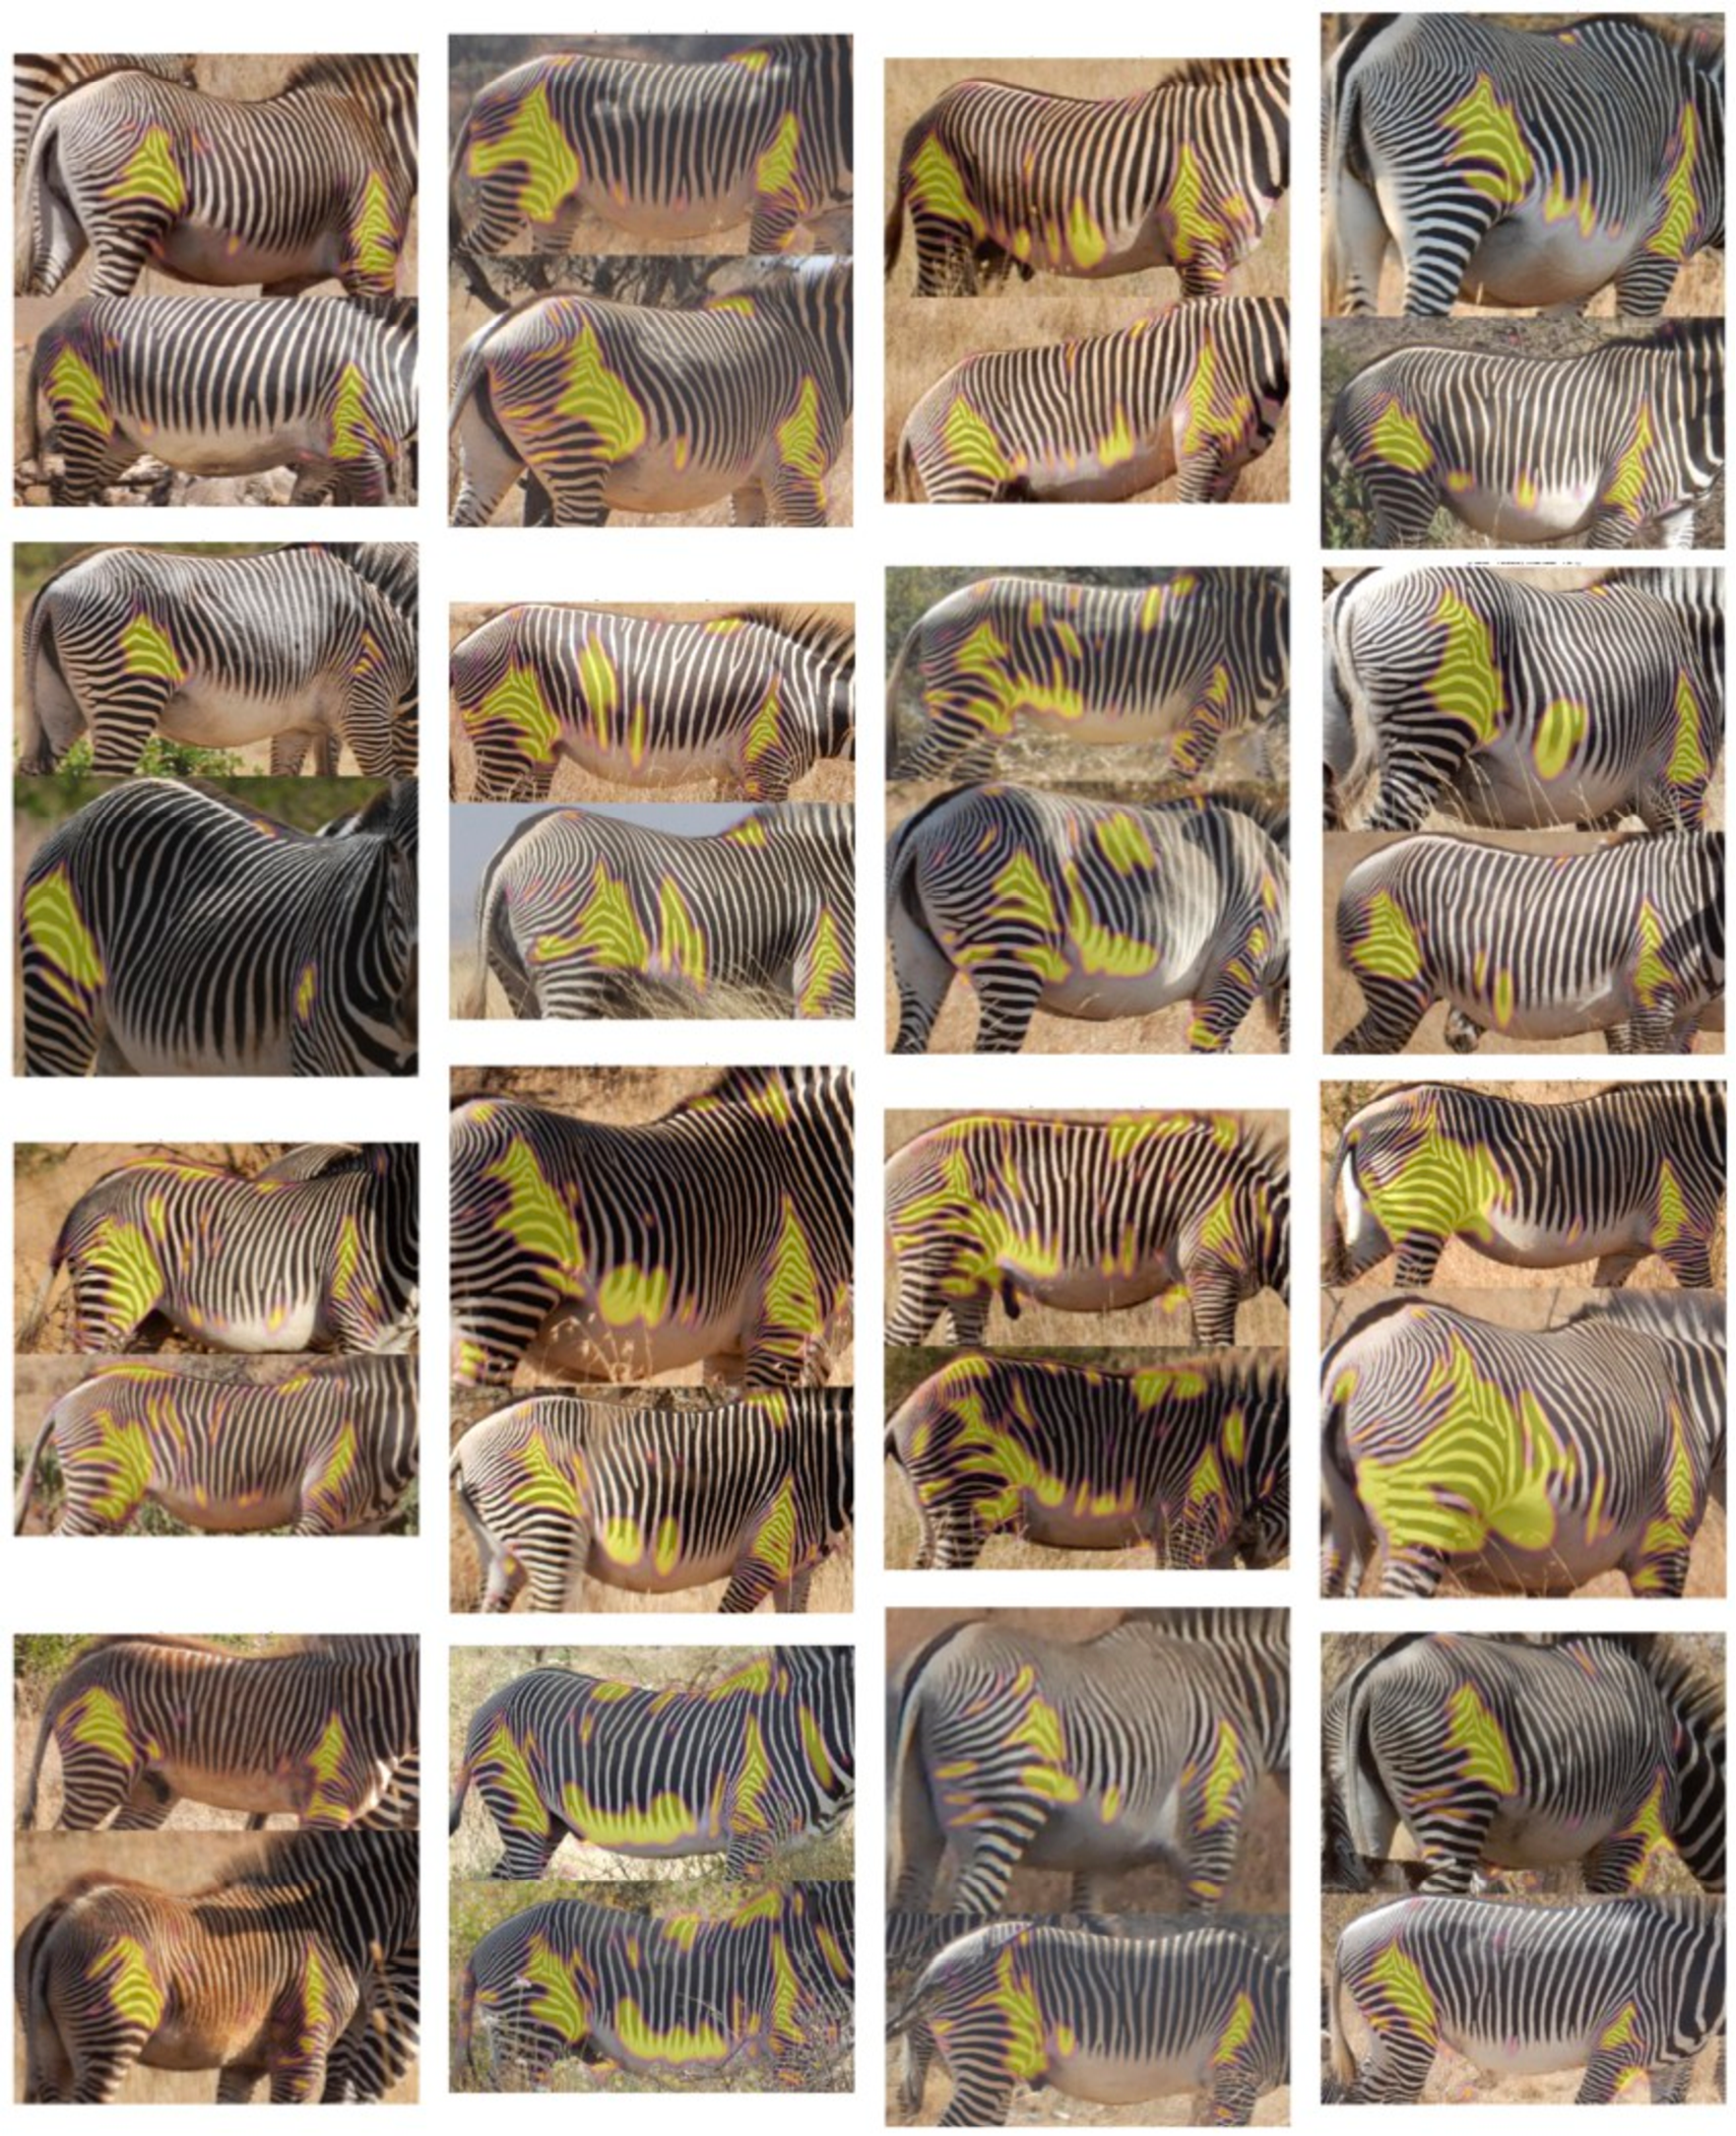
\includegraphics[width=0.85\linewidth]{resources/ca_regions_examples.pdf}
    \end{center}
    \caption{Example images of HotSpotter matched regions (in yellow) for Gr\'evy's Zebra.  The HotSpotter algorithm automatically finds corresponding texture patterns between two images and ranks likely matches.  The regions that tend to match strongly for Gr\'evy's zebra are the hip and shoulder areas, which are highlighted uniformly for all examples.  The concepts of Census Annotation and Census Annotation Regions (also shown here) are designed to focus a photographic census on the most likely matching areas while also removing distracting background textures from plants and animals.}
    \label{fig:ca-region-examples}
\end{figure}

Figure~\ref{fig:ca-sim-humans} shows the simulated results with a human error rate ranging from 50\% to 100\%.  All previous simulation ``baseline'' results for this configuration are shown as a red line and converge after 120 human decisions.  As expected, when the accuracy of the human verifier drops, the total number of reviews increases.  Encouragingly, however, the number of human decisions only increases by about one-third.  This effect is seen down to a human accuracy of 85\% and achieves the same result as the 100\% simulation.  This result is hopeful since it suggests that photographic censusing with LCA is fairly fault-tolerant and can accept human error with a healthy margin to spare for an individual user's ability.  At 80\% human accuracy, we start to notice a decrease in overall accuracy by 2-4\% and a significant drop-off in performance at 75\%.  Interestingly, the LCA algorithm still converges when the human verifier is 50\% accurate (a coin flip).  The problem is that the GGR-16 population estimate is 14.5\% under-counting, and the GGR-18 estimate is incorrect by -10\%.  An accurate human verifier is therefore crucial to the reliability and automation of photographic censusing.  These effects, while not tested, will only be exacerbated with the CA and ``Quality Baseline'' sets and will be much more devastating to reducing the overall workloads with the Graph ID algorithm.  As the best-case scenario, the comparison provided here demonstrates that a minimum human accuracy of 90\% is an acceptable target for practical use.  Similar to the loss of accuracy when the CA classifier was run at 90\%, if the accuracy of the human reviewers drops too low, then Assumption 3 (see Section~\ref{sec:assumptions}) begins to break as the inter-encounter recall is no longer perfect.

\section{Summary}

Census Annotations and Census Annotation Regions are critical to automated photographic census because they 1) speed up human verification of match pairs and reduce the number of manual decision errors, 2) better separate the positive and negative scores predicted by algorithmic verifiers, 3) reduce the number of photobombs and scenery matches, and 4) drastically reduce the amount of human interaction needed during animal ID curation.  Census Annotation Regions are powerful because they force a photographic census to consider only the most critical information for matching, as seen in Figure~\ref{fig:ca-region-examples}.

In summary, human verifiers can make 40\% more decisions in the same time frame when comparing Gr\'evy's zebra CA-Rs and make 70\% fewer mistakes. However, human verifiers are also known to make mistakes up to an error rate of 10\%.  A human accuracy rate of 90\% has been shown with simulations to only increase work by approximately 30\% and end with a consistent result (compared to a perfect verifier).  The VAMP verification algorithm can automatically decide -- given a maximum false-positive error rate -- 10\% more pair decisions when CAs are used and 15\% more with CA-Rs, compared to using the standard annotations produced by the detector.  Furthermore, CA-Rs dramatically improve the automated score separation for known cases of incidental matching, increasing the distance between the average positive and negative scores by 77\% for photobombs and 84\% for scenery matches.

Finally, simulations with Census Annotations and Census Annotation Regions demonstrate that using those annotations results in consistent population estimates compared to a known baseline. For example, a photographic census with CA-Rs uses 70\% fewer human decisions than the quality baseline and only increases the population estimate error by 0.5\% for GGR-16 and 0.3\% for GGR-18 while also remaining inside the expected confidence interval.  When we consider the number of decisions needed to arrive at these estimates, LCA with CA-R only required 120 human decisions for a database of 468 ground-truth IDs (0.26 decisions per ID).  Furthermore, the 120 human decisions were in addition to 13,307 automated reviews, indicating a decision automation rate of 99.1\%.  Using LCA with the quality baseline annotations results in 420 human decisions against 22,552 automated decisions (98.2\% automated).  In contrast, the baseline Graph ID algorithm with the baseline annotations approximated the population estimate with 2,414 human decisions for 487 IDs (4.96 decisions per ID).  That result was generated with only 12,988 requested automated reviews, an automation rate of 84.3\%.  Likewise, the Graph ID simulation with CA-R had 642 human decisions out of 5,553 total decisions (88.4\% automated).  These results indicate that using CA-R increases the automation of ID curation and dramatically reduces the number of automated reviews that are needed.

The next chapter will reveal the details of the Great Gr\'evy's Rally and the procedure used in 2016 and 2018 to provide a population estimate.  The original process used for those photographic censusing events did not include Census Annotations, Census Annotation Regions, or LCA. However, a culminating experiment is provided that shows the intended use case and most up-to-date procedure.
